% Options for packages loaded elsewhere
\PassOptionsToPackage{unicode}{hyperref}
\PassOptionsToPackage{hyphens}{url}
%
\documentclass[
]{book}
\usepackage{lmodern}
\usepackage{amssymb,amsmath}
\usepackage{ifxetex,ifluatex}
\ifnum 0\ifxetex 1\fi\ifluatex 1\fi=0 % if pdftex
  \usepackage[T1]{fontenc}
  \usepackage[utf8]{inputenc}
  \usepackage{textcomp} % provide euro and other symbols
\else % if luatex or xetex
  \usepackage{unicode-math}
  \defaultfontfeatures{Scale=MatchLowercase}
  \defaultfontfeatures[\rmfamily]{Ligatures=TeX,Scale=1}
\fi
% Use upquote if available, for straight quotes in verbatim environments
\IfFileExists{upquote.sty}{\usepackage{upquote}}{}
\IfFileExists{microtype.sty}{% use microtype if available
  \usepackage[]{microtype}
  \UseMicrotypeSet[protrusion]{basicmath} % disable protrusion for tt fonts
}{}
\makeatletter
\@ifundefined{KOMAClassName}{% if non-KOMA class
  \IfFileExists{parskip.sty}{%
    \usepackage{parskip}
  }{% else
    \setlength{\parindent}{0pt}
    \setlength{\parskip}{6pt plus 2pt minus 1pt}}
}{% if KOMA class
  \KOMAoptions{parskip=half}}
\makeatother
\usepackage{xcolor}
\IfFileExists{xurl.sty}{\usepackage{xurl}}{} % add URL line breaks if available
\IfFileExists{bookmark.sty}{\usepackage{bookmark}}{\usepackage{hyperref}}
\hypersetup{
  pdftitle={R Recipes for Common Medical Projects},
  hidelinks,
  pdfcreator={LaTeX via pandoc}}
\urlstyle{same} % disable monospaced font for URLs
\usepackage{color}
\usepackage{fancyvrb}
\newcommand{\VerbBar}{|}
\newcommand{\VERB}{\Verb[commandchars=\\\{\}]}
\DefineVerbatimEnvironment{Highlighting}{Verbatim}{commandchars=\\\{\}}
% Add ',fontsize=\small' for more characters per line
\usepackage{framed}
\definecolor{shadecolor}{RGB}{248,248,248}
\newenvironment{Shaded}{\begin{snugshade}}{\end{snugshade}}
\newcommand{\AlertTok}[1]{\textcolor[rgb]{0.94,0.16,0.16}{#1}}
\newcommand{\AnnotationTok}[1]{\textcolor[rgb]{0.56,0.35,0.01}{\textbf{\textit{#1}}}}
\newcommand{\AttributeTok}[1]{\textcolor[rgb]{0.77,0.63,0.00}{#1}}
\newcommand{\BaseNTok}[1]{\textcolor[rgb]{0.00,0.00,0.81}{#1}}
\newcommand{\BuiltInTok}[1]{#1}
\newcommand{\CharTok}[1]{\textcolor[rgb]{0.31,0.60,0.02}{#1}}
\newcommand{\CommentTok}[1]{\textcolor[rgb]{0.56,0.35,0.01}{\textit{#1}}}
\newcommand{\CommentVarTok}[1]{\textcolor[rgb]{0.56,0.35,0.01}{\textbf{\textit{#1}}}}
\newcommand{\ConstantTok}[1]{\textcolor[rgb]{0.00,0.00,0.00}{#1}}
\newcommand{\ControlFlowTok}[1]{\textcolor[rgb]{0.13,0.29,0.53}{\textbf{#1}}}
\newcommand{\DataTypeTok}[1]{\textcolor[rgb]{0.13,0.29,0.53}{#1}}
\newcommand{\DecValTok}[1]{\textcolor[rgb]{0.00,0.00,0.81}{#1}}
\newcommand{\DocumentationTok}[1]{\textcolor[rgb]{0.56,0.35,0.01}{\textbf{\textit{#1}}}}
\newcommand{\ErrorTok}[1]{\textcolor[rgb]{0.64,0.00,0.00}{\textbf{#1}}}
\newcommand{\ExtensionTok}[1]{#1}
\newcommand{\FloatTok}[1]{\textcolor[rgb]{0.00,0.00,0.81}{#1}}
\newcommand{\FunctionTok}[1]{\textcolor[rgb]{0.00,0.00,0.00}{#1}}
\newcommand{\ImportTok}[1]{#1}
\newcommand{\InformationTok}[1]{\textcolor[rgb]{0.56,0.35,0.01}{\textbf{\textit{#1}}}}
\newcommand{\KeywordTok}[1]{\textcolor[rgb]{0.13,0.29,0.53}{\textbf{#1}}}
\newcommand{\NormalTok}[1]{#1}
\newcommand{\OperatorTok}[1]{\textcolor[rgb]{0.81,0.36,0.00}{\textbf{#1}}}
\newcommand{\OtherTok}[1]{\textcolor[rgb]{0.56,0.35,0.01}{#1}}
\newcommand{\PreprocessorTok}[1]{\textcolor[rgb]{0.56,0.35,0.01}{\textit{#1}}}
\newcommand{\RegionMarkerTok}[1]{#1}
\newcommand{\SpecialCharTok}[1]{\textcolor[rgb]{0.00,0.00,0.00}{#1}}
\newcommand{\SpecialStringTok}[1]{\textcolor[rgb]{0.31,0.60,0.02}{#1}}
\newcommand{\StringTok}[1]{\textcolor[rgb]{0.31,0.60,0.02}{#1}}
\newcommand{\VariableTok}[1]{\textcolor[rgb]{0.00,0.00,0.00}{#1}}
\newcommand{\VerbatimStringTok}[1]{\textcolor[rgb]{0.31,0.60,0.02}{#1}}
\newcommand{\WarningTok}[1]{\textcolor[rgb]{0.56,0.35,0.01}{\textbf{\textit{#1}}}}
\usepackage{longtable,booktabs}
% Correct order of tables after \paragraph or \subparagraph
\usepackage{etoolbox}
\makeatletter
\patchcmd\longtable{\par}{\if@noskipsec\mbox{}\fi\par}{}{}
\makeatother
% Allow footnotes in longtable head/foot
\IfFileExists{footnotehyper.sty}{\usepackage{footnotehyper}}{\usepackage{footnote}}
\makesavenoteenv{longtable}
\usepackage{graphicx,grffile}
\makeatletter
\def\maxwidth{\ifdim\Gin@nat@width>\linewidth\linewidth\else\Gin@nat@width\fi}
\def\maxheight{\ifdim\Gin@nat@height>\textheight\textheight\else\Gin@nat@height\fi}
\makeatother
% Scale images if necessary, so that they will not overflow the page
% margins by default, and it is still possible to overwrite the defaults
% using explicit options in \includegraphics[width, height, ...]{}
\setkeys{Gin}{width=\maxwidth,height=\maxheight,keepaspectratio}
% Set default figure placement to htbp
\makeatletter
\def\fps@figure{htbp}
\makeatother
\setlength{\emergencystretch}{3em} % prevent overfull lines
\providecommand{\tightlist}{%
  \setlength{\itemsep}{0pt}\setlength{\parskip}{0pt}}
\setcounter{secnumdepth}{5}
\usepackage{booktabs}
\usepackage{longtable}
\usepackage{makeidx}
\makeindex
\usepackage[]{natbib}
\bibliographystyle{apalike}

\title{R Recipes for Common Medical Projects}
\author{}
\date{\vspace{-2.5em}}

\begin{document}
\maketitle

{
\setcounter{tocdepth}{3}
\tableofcontents
}
\hypertarget{section}{%
\chapter*{}\label{section}}
\addcontentsline{toc}{chapter}{}

\hypertarget{preface}{%
\chapter*{Preface}\label{preface}}
\addcontentsline{toc}{chapter}{Preface}

This book contains R recipes for typical analyses done for medical research projects. The objectives of this book:

\begin{itemize}
\tightlist
\item
  Create Mock projects and analyze the data using R
\item
  Give people code snippets that they can use for their own projects
\item
  Show how the various packages and functions fit together
\item
  Recommend key packages for summarizing data
\item
  Provide links for further study
\item
  Model best practices for coding
\item
  Encourage the use of RStudio and R markdown
\end{itemize}

The assumption is that users will have some basic knowledge of R. Instead of re-creating introductory information or extended lists of options, we have chosen to provide one way of doing the analysis (with a perhaps a few more at the end of each scenario). Links are provided to other resources for more education.

\hypertarget{getting-started}{%
\section{Getting Started}\label{getting-started}}

\begin{itemize}
\item
  Although not required, we strongly encourage that users work through these examples using RStudio. RStudio is an integrated environment that includes an editor to write code, a console to execute code, a workspace to view objects in your session, a help window, and much more. Information on using RStudio can be found at \url{https://moderndive.netlify.com/1-getting-started.html}.
\item
  Most of the functions used in this book are from base R or tidyverse packages (other packages will be described, when used, throughout this book). Direct links to packages used for each scenario are included at the end of the scenarios.

  \begin{itemize}
  \tightlist
  \item
    Tidyverse is a collection of packages designed to work together to solve data science problems. The figure below includes the stages of an analysis and the tidyverse packages developed for each stage.
  \end{itemize}
\end{itemize}

\begin{center}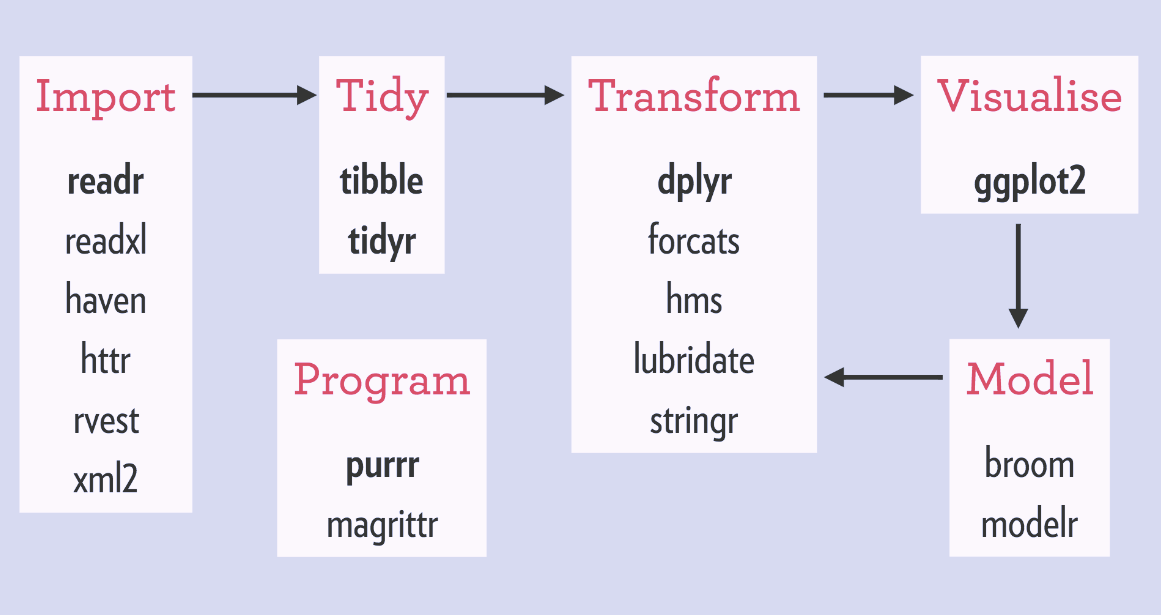
\includegraphics[width=0.8\linewidth]{images/Tidyverse} \end{center}

Core tidyverse packages can be loaded into your R session with \texttt{library(tidyverse)}. The function \texttt{tidyverse\_packages()} details what packages are in the \texttt{tidyverse} while the \texttt{search()} command shows what packages have been loaded. There are additional packages that are considered a part of the tidyverse that are not automatically loaded. Highlights of some of the key tidyverse packages are shown in the appendix.

\begin{Shaded}
\begin{Highlighting}[]
\OperatorTok{>}\StringTok{ }\KeywordTok{library}\NormalTok{(tidyverse)  }\CommentTok{# load basic tidyverse packages}
\OperatorTok{>}\StringTok{ }\KeywordTok{search}\NormalTok{()  }\CommentTok{# see what was loaded}
\NormalTok{ [}\DecValTok{1}\NormalTok{] }\StringTok{".GlobalEnv"}        \StringTok{"package:forcats"}   \StringTok{"package:stringr"}  
\NormalTok{ [}\DecValTok{4}\NormalTok{] }\StringTok{"package:dplyr"}     \StringTok{"package:purrr"}     \StringTok{"package:readr"}    
\NormalTok{ [}\DecValTok{7}\NormalTok{] }\StringTok{"package:tidyr"}     \StringTok{"package:tibble"}    \StringTok{"package:ggplot2"}  
\NormalTok{[}\DecValTok{10}\NormalTok{] }\StringTok{"package:tidyverse"} \StringTok{"package:stats"}     \StringTok{"package:graphics"} 
\NormalTok{[}\DecValTok{13}\NormalTok{] }\StringTok{"package:grDevices"} \StringTok{"package:utils"}     \StringTok{"package:datasets"} 
\NormalTok{[}\DecValTok{16}\NormalTok{] }\StringTok{"package:methods"}   \StringTok{"Autoloads"}         \StringTok{"package:base"}     
\OperatorTok{>}\StringTok{ }
\ErrorTok{>}\StringTok{ }\KeywordTok{tidyverse_packages}\NormalTok{(}\DataTypeTok{include_self =} \OtherTok{TRUE}\NormalTok{)  }\CommentTok{# list all packages in tidyverse}
\NormalTok{ [}\DecValTok{1}\NormalTok{] }\StringTok{"broom"}      \StringTok{"cli"}        \StringTok{"crayon"}     \StringTok{"dbplyr"}     \StringTok{"dplyr"}     
\NormalTok{ [}\DecValTok{6}\NormalTok{] }\StringTok{"forcats"}    \StringTok{"ggplot2"}    \StringTok{"haven"}      \StringTok{"hms"}        \StringTok{"httr"}      
\NormalTok{[}\DecValTok{11}\NormalTok{] }\StringTok{"jsonlite"}   \StringTok{"lubridate"}  \StringTok{"magrittr"}   \StringTok{"modelr"}     \StringTok{"pillar"}    
\NormalTok{[}\DecValTok{16}\NormalTok{] }\StringTok{"purrr"}      \StringTok{"readr"}      \StringTok{"readxl"}     \StringTok{"reprex"}     \StringTok{"rlang"}     
\NormalTok{[}\DecValTok{21}\NormalTok{] }\StringTok{"rstudioapi"} \StringTok{"rvest"}      \StringTok{"stringr"}    \StringTok{"tibble"}     \StringTok{"tidyr"}     
\NormalTok{[}\DecValTok{26}\NormalTok{] }\StringTok{"xml2"}       \StringTok{"tidyverse"} 
\end{Highlighting}
\end{Shaded}

\hypertarget{r-markdown}{%
\section{R markdown}\label{r-markdown}}

R markdown (file extention \texttt{.Rmd}) is a simple way to integrate R output and text, then output as HTML, PDF, or Word. The syntax is pretty basic (e.g., a bulleted list is simply an astrix \texttt{*} followed by text). R markdown is much easier to compile and explore using RStudio, thought it can be run using R from a terminal window. There is a lot of documentation available on getting started with R Markdown including:

\begin{itemize}
\tightlist
\item
  \href{https://www.rstudio.com/resources/cheatsheets/}{RStudio cheatsheets}
\item
  \href{https://www.rstudio.com/resources/webinars/}{RStudio webinar archives}
\end{itemize}

\hypertarget{the-data}{%
\section{The Data}\label{the-data}}

There are separate datasets used for each scenario. They are based on real data but certain variables are simulated or perturbed. Patient ID numbers have all been fabricated.

You can try the exercises out by first \href{}{downloading the data} to your home directory or read in the data from the Github page using the provided code. The exercises assume that you have the files in a subdirectory called ``data'' that is in the same directory as your programs.

\hypertarget{scenarios}{%
\section{Scenarios}\label{scenarios}}

Scenario 1: Getting Familiar with a New Project

\begin{itemize}
\tightlist
\item
  In this scenario, you are starting a new project and want to get familiar with the data. It covers:

  \begin{itemize}
  \tightlist
  \item
    Import Data
  \item
    Explore Data
    + Identify and deal with strange values and duplicate observations
    + Generate summary statistics
  \item
    Plot Data
  \item
    Fit a simple model
  \end{itemize}
\end{itemize}

Scenario 2: Modeling and Plotting with Cleaned Data

\begin{itemize}
\tightlist
\item
  In this scenario, you already cleaned your data but want to do more complex models and plots.

  \begin{itemize}
  \tightlist
  \item
    Deal with missing data
  \item
    Plot Kaplan Meier \& cumulative incidence curves
  \item
    Run linear, logistic \& Cox models
  \end{itemize}
\end{itemize}

Scenario 3: Working with Multiple Observations per Subject

\begin{itemize}
\tightlist
\item
  In this scenario you will work with multiple observations per subject as is often found in longitudinal data.

  \begin{itemize}
  \tightlist
  \item
    Explore and clean baseline data
  \item
    Using a cleaned version of the full dataset (up to 4 visits per subject), transform the data from 1 obs/subject to 1 obs/subject/visit.
  \item
    Plot the data with separate lines for each subject
  \item
    Fit linear models and linear mixed effects models
  \end{itemize}
\end{itemize}

\hypertarget{finding-help}{%
\section{Finding help}\label{finding-help}}

There are several ways to find additional help.

\begin{itemize}
\tightlist
\item
  Using the help function. These are to remind the user of the argument names, but are not extensive.
\end{itemize}

\begin{verbatim}
help(foo)       # brief help/syntax about function foo
?foo            # same thing
example(foo)    # show an example of function foo
apropos("foo")  # list all functions containing the string "foo"
\end{verbatim}

\begin{itemize}
\tightlist
\item
  Vignettes. These generally provide more detailed examples if they are available.
\end{itemize}

\begin{verbatim}
vignette()         # show available vignettes in loaded packages
vignette("foo")    # show specific vignette
\end{verbatim}

Or search the web for ``R vignette foo''

\begin{itemize}
\tightlist
\item
  Try one these sites

  \begin{itemize}
  \tightlist
  \item
    \href{https://www.statmethods.net/index.html}{Quick-R}
  \item
    \href{https://stackoverflow.com/}{stack overflow}
  \item
    \href{http://www.sthda.com/english/}{Statistical tools for high-throughput data analysis (STHDA)}
  \item
    \href{https://www.rstudio.com/resources/cheatsheets/}{Use package cheat sheets}
  \item
    \href{https://www.rstudio.com/online-learning/}{RStudio Online Learning}
  \end{itemize}
\item
  Google tips

  \begin{itemize}
  \tightlist
  \item
    Use key ``R'' words like ggplot: \href{https://www.google.com/search?q=ggplot+add+horizontal+line}{ggplot add horizontal line}
  \item
    Check the date of the posting, especially for code relating to the tidyverse. It is still relatively new and the coding has changed over time.
  \end{itemize}
\end{itemize}

\hypertarget{disclosure}{%
\section{Disclosure}\label{disclosure}}

The solutions presented here are one way to do things (usually the ``easy'' way), and there was a lot of discussion about which was the ``easy'' way. Alternative solutions are presented in the appendix.

\hypertarget{contributors}{%
\section{Contributors}\label{contributors}}

This series of examples was created by Beth Atkinson, Brendan Broderick, Erin Carlson, Krista Goergen, Mike Golafshar, Ethan Heinzen, Katie Kunze, Liz Lesser, Peter Martin, Ryan Lennon.

\hypertarget{scenario-1-getting-familiar-with-a-new-project}{%
\chapter{Scenario 1: Getting Familiar with a New Project}\label{scenario-1-getting-familiar-with-a-new-project}}

You're handed a new project to work on and the abstract deadline is next week. You need to get something out the door soon!

\hypertarget{your-mission}{%
\section{Your Mission}\label{your-mission}}

\textbf{Import Data}

\begin{itemize}
\tightlist
\item
  Read in the example dataset dat1.sas7bdat. What variables are in the data? Are they character, numeric, Date, or factor?
\end{itemize}

\textbf{Explore Data}

\begin{itemize}
\tightlist
\item
  Take a closer look at the data using basic summary statistics. Do you notice any strange values? If so, fix them. Are there any duplicate observations? If so, see whether you can delete any of them.
\item
  Summarize age, gender, bmi, etc. by the treatment variable using parametric statistics. Do the summary statistics make sense for each variable? If not, modify the variables so that the default summaries are appropriate.
\item
  Change the label for the variable age. Now change the table summary statistics to be non-parametric.
\item
  How many people have the combinations of ps, sex, and treatment arm?
\item
  Create a formula from a list of variables that can used in tableby (hint: try \texttt{formulize})
\end{itemize}

\textbf{Plot Data}

\begin{itemize}
\tightlist
\item
  Create a boxplot of bmi. Now create the boxplots stratified by the treatment arm. Modify the axis labels and add a title to your plot.
\item
  Create a scatterplot of age versus another continuous variable. Now create the plot with separate colors for one of the group variables. Now make two scatterplots of age versus bmi with different colors indicating treatment.
\item
  Create these same scatterplots, side-by-side, separately for males and females. How would you add a regression line to these plots? How about smoothers?
\end{itemize}

\textbf{Basic Modeling}

\begin{itemize}
\tightlist
\item
  Run a simple linear regression model predicting bmi with a covariate that is coded as 1/2.
  Now re-do it with the covariate coded as a factor. Did the answer change?
\end{itemize}

\textbf{Data Import, revisited}

\begin{itemize}
\tightlist
\item
  Read the data in from Excel and compare it with the version that came from SAS. What is different?
\end{itemize}

\hypertarget{implementation}{%
\section{Implementation}\label{implementation}}

\hypertarget{import-data}{%
\subsection{Import Data}\label{import-data}}

\begin{itemize}
\tightlist
\item
  \textbf{Read in the example dataset dat1.sas7bdat.}
\item
  \textbf{What variables are in the data? Are they character, numeric, Date, or factor? }
\end{itemize}

When reading in SAS data you can use the \texttt{read\_sas()} function that is found in the \texttt{haven} package. To make a package available simply use the \texttt{library()} function with the non-quoted name of the package. The \texttt{read\_sas()} function works for the majority of SAS datasets. Other options are found at the \protect\hyperlink{alt-import}{end of this document} in the rare situations where you need to use a different tool.

\begin{Shaded}
\begin{Highlighting}[]
\OperatorTok{>}\StringTok{ }\CommentTok{# Before doing any work, you are strongly encouraged to set this option in each}
\ErrorTok{>}\StringTok{ }\CommentTok{# of your programs (default for later versions of R)}
\ErrorTok{>}\StringTok{ }\KeywordTok{options}\NormalTok{(}\DataTypeTok{stringsAsFactors =} \OtherTok{FALSE}\NormalTok{)}
\OperatorTok{>}\StringTok{ }
\ErrorTok{>}\StringTok{ }\CommentTok{# various functions from the tidyverse package are used.  You can safely ignore}
\ErrorTok{>}\StringTok{ }\CommentTok{# the messages regarding conflicts for now}
\ErrorTok{>}\StringTok{ }\KeywordTok{library}\NormalTok{(tidyverse)}
\OperatorTok{>}\StringTok{ }\CommentTok{# use the read_sas function found in the haven package}
\ErrorTok{>}\StringTok{ }\KeywordTok{library}\NormalTok{(haven)}
\OperatorTok{>}\StringTok{ }\CommentTok{# the knitr package includes the kable function for simple nice tables}
\ErrorTok{>}\StringTok{ }\KeywordTok{library}\NormalTok{(knitr)}
\OperatorTok{>}\StringTok{ }
\ErrorTok{>}\StringTok{ }\CommentTok{# link to data on GitHub page if not already downloaded}
\ErrorTok{>}\StringTok{ }\ControlFlowTok{if}\NormalTok{ (}\OperatorTok{!}\KeywordTok{file.exists}\NormalTok{(}\StringTok{"data/dat1.sas7bdat"}\NormalTok{)) \{}
\OperatorTok{+}\StringTok{     }\NormalTok{urlfile <-}\StringTok{ "https://raw.githubusercontent.com/bethatkinson/R_project_recipes/data/dat1.sas7bdat"}
\OperatorTok{+}\StringTok{     }\ControlFlowTok{if}\NormalTok{ (}\OperatorTok{!}\KeywordTok{dir.exists}\NormalTok{(}\StringTok{"data"}\NormalTok{)) }
\OperatorTok{+}\StringTok{         }\KeywordTok{dir.create}\NormalTok{(}\StringTok{"data"}\NormalTok{)}
\OperatorTok{+}\StringTok{     }\KeywordTok{download.file}\NormalTok{(urlfile, }\DataTypeTok{destfile =} \StringTok{"data/dat1.sas7bdat"}\NormalTok{)}
\OperatorTok{+}\StringTok{ }\NormalTok{\}}
\OperatorTok{>}\StringTok{ }
\ErrorTok{>}\StringTok{ }\NormalTok{dat1 <-}\StringTok{ }\KeywordTok{read_sas}\NormalTok{(}\StringTok{"data/dat1.sas7bdat"}\NormalTok{)}
\end{Highlighting}
\end{Shaded}

Once we successfully import data into the current R session we should explore it a little bit. The \texttt{names()} function is a good first step as it displays all the column names of the data, and you can quickly check to see if your import went as expected.

\begin{itemize}
\tightlist
\item
  \texttt{names()} returns a character vector
\end{itemize}

\begin{Shaded}
\begin{Highlighting}[]
\OperatorTok{>}\StringTok{ }\KeywordTok{names}\NormalTok{(dat1)}
\NormalTok{ [}\DecValTok{1}\NormalTok{] }\StringTok{"id"}         \StringTok{"age"}        \StringTok{"arm"}        \StringTok{"sex"}        \StringTok{"futime"}    
\NormalTok{ [}\DecValTok{6}\NormalTok{] }\StringTok{"fustat"}     \StringTok{"ps"}         \StringTok{"hgb"}        \StringTok{"bmi"}        \StringTok{"alkphos"}   
\NormalTok{[}\DecValTok{11}\NormalTok{] }\StringTok{"ast"}        \StringTok{"mdqualitys"} \StringTok{"ageord"}     \StringTok{"birthdt"}    \StringTok{"resintdt"}  
\end{Highlighting}
\end{Shaded}

To understand how many observations are in your data, we can use \texttt{nrow()} function. Similarly, we can also print the number of columns with \texttt{ncol()}. The function \texttt{dim()} returns both the number of rows and columns at once.

\begin{itemize}
\tightlist
\item
  \texttt{nrow()} and \texttt{ncol()} return integers
\item
  \texttt{dim()} returns a vector (rows, columns)
\end{itemize}

\begin{Shaded}
\begin{Highlighting}[]
\OperatorTok{>}\StringTok{ }\CommentTok{# how many rows and columns are in the dataset?}
\ErrorTok{>}\StringTok{ }\KeywordTok{nrow}\NormalTok{(dat1)}
\NormalTok{[}\DecValTok{1}\NormalTok{] }\DecValTok{890}
\OperatorTok{>}\StringTok{ }\KeywordTok{ncol}\NormalTok{(dat1)}
\NormalTok{[}\DecValTok{1}\NormalTok{] }\DecValTok{15}
\OperatorTok{>}\StringTok{ }\KeywordTok{dim}\NormalTok{(dat1)}
\NormalTok{[}\DecValTok{1}\NormalTok{] }\DecValTok{890}  \DecValTok{15}
\end{Highlighting}
\end{Shaded}

Another really useful function to use to explore data is the \texttt{str()} or ``structure'' function. When we run it, we can see all of the column names like the \texttt{names()} function, but now we also see the type of each column as well as any attributes that a column has. The \texttt{read\_sas()} function reads in the format and label metadata used in SAS datasets as R object attributes. It is worth noting that the \texttt{str()} function works on most R objects, not just \texttt{data.frames}.

\begin{Shaded}
\begin{Highlighting}[]
\OperatorTok{>}\StringTok{ }\KeywordTok{str}\NormalTok{(dat1)}
\NormalTok{tibble [}\DecValTok{890}\NormalTok{ x }\DecValTok{15}\NormalTok{] (S3}\OperatorTok{:}\StringTok{ }\NormalTok{tbl_df}\OperatorTok{/}\NormalTok{tbl}\OperatorTok{/}\NormalTok{data.frame)}
 \OperatorTok{$}\StringTok{ }\NormalTok{id        }\OperatorTok{:}\StringTok{ }\NormalTok{num [}\DecValTok{1}\OperatorTok{:}\DecValTok{890}\NormalTok{] }\DecValTok{84681} \DecValTok{89253} \DecValTok{89499} \DecValTok{90166} \DecValTok{90291}\NormalTok{ ...}
\NormalTok{  ..}\OperatorTok{-}\StringTok{ }\KeywordTok{attr}\NormalTok{(}\OperatorTok{*}\NormalTok{, }\StringTok{"format.sas"}\NormalTok{)=}\StringTok{ }\NormalTok{chr }\StringTok{"BEST"}
 \OperatorTok{$}\StringTok{ }\NormalTok{age       }\OperatorTok{:}\StringTok{ }\NormalTok{num [}\DecValTok{1}\OperatorTok{:}\DecValTok{890}\NormalTok{] }\DecValTok{57} \DecValTok{64} \DecValTok{75} \DecValTok{54} \DecValTok{71} \DecValTok{71} \DecValTok{66} \DecValTok{56} \DecValTok{50} \DecValTok{43}\NormalTok{ ...}
\NormalTok{  ..}\OperatorTok{-}\StringTok{ }\KeywordTok{attr}\NormalTok{(}\OperatorTok{*}\NormalTok{, }\StringTok{"format.sas"}\NormalTok{)=}\StringTok{ }\NormalTok{chr }\StringTok{"BEST"}
 \OperatorTok{$}\StringTok{ }\NormalTok{arm       }\OperatorTok{:}\StringTok{ }\NormalTok{chr [}\DecValTok{1}\OperatorTok{:}\DecValTok{890}\NormalTok{] }\StringTok{"F FOLFOX"} \StringTok{"F FOLFOX"} \StringTok{"F FOLFOX"} \StringTok{"G IROX"}\NormalTok{ ...}
\NormalTok{  ..}\OperatorTok{-}\StringTok{ }\KeywordTok{attr}\NormalTok{(}\OperatorTok{*}\NormalTok{, }\StringTok{"label"}\NormalTok{)=}\StringTok{ }\NormalTok{chr }\StringTok{"Treatment Arm"}
\NormalTok{  ..}\OperatorTok{-}\StringTok{ }\KeywordTok{attr}\NormalTok{(}\OperatorTok{*}\NormalTok{, }\StringTok{"format.sas"}\NormalTok{)=}\StringTok{ }\NormalTok{chr }\StringTok{"$"}
 \OperatorTok{$}\StringTok{ }\NormalTok{sex       }\OperatorTok{:}\StringTok{ }\NormalTok{chr [}\DecValTok{1}\OperatorTok{:}\DecValTok{890}\NormalTok{] }\StringTok{"Male"} \StringTok{"Female"} \StringTok{"Female"} \StringTok{"Female"}\NormalTok{ ...}
\NormalTok{  ..}\OperatorTok{-}\StringTok{ }\KeywordTok{attr}\NormalTok{(}\OperatorTok{*}\NormalTok{, }\StringTok{"format.sas"}\NormalTok{)=}\StringTok{ }\NormalTok{chr }\StringTok{"$"}
 \OperatorTok{$}\StringTok{ }\NormalTok{futime    }\OperatorTok{:}\StringTok{ }\NormalTok{num [}\DecValTok{1}\OperatorTok{:}\DecValTok{890}\NormalTok{] }\DecValTok{799} \DecValTok{97} \DecValTok{105} \DecValTok{878} \DecValTok{31}\NormalTok{ ...}
\NormalTok{  ..}\OperatorTok{-}\StringTok{ }\KeywordTok{attr}\NormalTok{(}\OperatorTok{*}\NormalTok{, }\StringTok{"label"}\NormalTok{)=}\StringTok{ }\NormalTok{chr }\StringTok{"Follow-up Time"}
\NormalTok{  ..}\OperatorTok{-}\StringTok{ }\KeywordTok{attr}\NormalTok{(}\OperatorTok{*}\NormalTok{, }\StringTok{"format.sas"}\NormalTok{)=}\StringTok{ }\NormalTok{chr }\StringTok{"BEST"}
 \OperatorTok{$}\StringTok{ }\NormalTok{fustat    }\OperatorTok{:}\StringTok{ }\NormalTok{num [}\DecValTok{1}\OperatorTok{:}\DecValTok{890}\NormalTok{] }\DecValTok{2} \DecValTok{2} \DecValTok{2} \DecValTok{2} \DecValTok{2} \DecValTok{1} \DecValTok{2} \DecValTok{2} \DecValTok{2} \DecValTok{2}\NormalTok{ ...}
\NormalTok{  ..}\OperatorTok{-}\StringTok{ }\KeywordTok{attr}\NormalTok{(}\OperatorTok{*}\NormalTok{, }\StringTok{"label"}\NormalTok{)=}\StringTok{ }\NormalTok{chr }\StringTok{"Follow-up Status"}
\NormalTok{  ..}\OperatorTok{-}\StringTok{ }\KeywordTok{attr}\NormalTok{(}\OperatorTok{*}\NormalTok{, }\StringTok{"format.sas"}\NormalTok{)=}\StringTok{ }\NormalTok{chr }\StringTok{"STATF"}
 \OperatorTok{$}\StringTok{ }\NormalTok{ps        }\OperatorTok{:}\StringTok{ }\NormalTok{num [}\DecValTok{1}\OperatorTok{:}\DecValTok{890}\NormalTok{] }\DecValTok{0} \DecValTok{1} \DecValTok{1} \DecValTok{0} \DecValTok{2} \OtherTok{NA} \DecValTok{1} \DecValTok{1} \DecValTok{1} \OtherTok{NA}\NormalTok{ ...}
\NormalTok{  ..}\OperatorTok{-}\StringTok{ }\KeywordTok{attr}\NormalTok{(}\OperatorTok{*}\NormalTok{, }\StringTok{"label"}\NormalTok{)=}\StringTok{ }\NormalTok{chr }\StringTok{"ECOG Performance Score"}
\NormalTok{  ..}\OperatorTok{-}\StringTok{ }\KeywordTok{attr}\NormalTok{(}\OperatorTok{*}\NormalTok{, }\StringTok{"format.sas"}\NormalTok{)=}\StringTok{ }\NormalTok{chr }\StringTok{"BEST"}
 \OperatorTok{$}\StringTok{ }\NormalTok{hgb       }\OperatorTok{:}\StringTok{ }\NormalTok{num [}\DecValTok{1}\OperatorTok{:}\DecValTok{890}\NormalTok{] }\FloatTok{11.2} \FloatTok{12.6} \FloatTok{12.5} \FloatTok{10.9} \FloatTok{9.1} \OtherTok{NA} \FloatTok{10.5} \FloatTok{10.8} \FloatTok{13.4} \OtherTok{NA}\NormalTok{ ...}
\NormalTok{  ..}\OperatorTok{-}\StringTok{ }\KeywordTok{attr}\NormalTok{(}\OperatorTok{*}\NormalTok{, }\StringTok{"label"}\NormalTok{)=}\StringTok{ }\NormalTok{chr }\StringTok{"Hemoglobin Count"}
\NormalTok{  ..}\OperatorTok{-}\StringTok{ }\KeywordTok{attr}\NormalTok{(}\OperatorTok{*}\NormalTok{, }\StringTok{"format.sas"}\NormalTok{)=}\StringTok{ }\NormalTok{chr }\StringTok{"BEST"}
 \OperatorTok{$}\StringTok{ }\NormalTok{bmi       }\OperatorTok{:}\StringTok{ }\NormalTok{num [}\DecValTok{1}\OperatorTok{:}\DecValTok{890}\NormalTok{] }\OtherTok{NA} \OtherTok{NA} \OtherTok{NA} \OtherTok{NA} \OtherTok{NA} \OtherTok{NA} \OtherTok{NA} \OtherTok{NA} \OtherTok{NA} \OtherTok{NA}\NormalTok{ ...}
\NormalTok{  ..}\OperatorTok{-}\StringTok{ }\KeywordTok{attr}\NormalTok{(}\OperatorTok{*}\NormalTok{, }\StringTok{"format.sas"}\NormalTok{)=}\StringTok{ }\NormalTok{chr }\StringTok{"BEST"}
 \OperatorTok{$}\StringTok{ }\NormalTok{alkphos   }\OperatorTok{:}\StringTok{ }\NormalTok{num [}\DecValTok{1}\OperatorTok{:}\DecValTok{890}\NormalTok{] }\DecValTok{102} \DecValTok{272} \DecValTok{169} \DecValTok{247} \DecValTok{304} \OtherTok{NA} \DecValTok{196} \DecValTok{252} \DecValTok{69} \OtherTok{NA}\NormalTok{ ...}
\NormalTok{  ..}\OperatorTok{-}\StringTok{ }\KeywordTok{attr}\NormalTok{(}\OperatorTok{*}\NormalTok{, }\StringTok{"label"}\NormalTok{)=}\StringTok{ }\NormalTok{chr }\StringTok{"Alkaline Phosphotase"}
\NormalTok{  ..}\OperatorTok{-}\StringTok{ }\KeywordTok{attr}\NormalTok{(}\OperatorTok{*}\NormalTok{, }\StringTok{"format.sas"}\NormalTok{)=}\StringTok{ }\NormalTok{chr }\StringTok{"BEST"}
 \OperatorTok{$}\StringTok{ }\NormalTok{ast       }\OperatorTok{:}\StringTok{ }\NormalTok{num [}\DecValTok{1}\OperatorTok{:}\DecValTok{890}\NormalTok{] }\DecValTok{7} \DecValTok{62} \DecValTok{23} \DecValTok{23} \DecValTok{115} \OtherTok{NA} \DecValTok{39} \DecValTok{77} \DecValTok{13} \OtherTok{NA}\NormalTok{ ...}
\NormalTok{  ..}\OperatorTok{-}\StringTok{ }\KeywordTok{attr}\NormalTok{(}\OperatorTok{*}\NormalTok{, }\StringTok{"label"}\NormalTok{)=}\StringTok{ }\NormalTok{chr }\StringTok{"Aspartate Transaminase"}
\NormalTok{  ..}\OperatorTok{-}\StringTok{ }\KeywordTok{attr}\NormalTok{(}\OperatorTok{*}\NormalTok{, }\StringTok{"format.sas"}\NormalTok{)=}\StringTok{ }\NormalTok{chr }\StringTok{"BEST"}
 \OperatorTok{$}\StringTok{ }\NormalTok{mdqualitys}\OperatorTok{:}\StringTok{ }\NormalTok{num [}\DecValTok{1}\OperatorTok{:}\DecValTok{890}\NormalTok{] }\OtherTok{NA} \DecValTok{1} \DecValTok{1} \DecValTok{1} \DecValTok{1} \DecValTok{1} \DecValTok{0} \DecValTok{1} \OtherTok{NA} \DecValTok{0}\NormalTok{ ...}
\NormalTok{  ..}\OperatorTok{-}\StringTok{ }\KeywordTok{attr}\NormalTok{(}\OperatorTok{*}\NormalTok{, }\StringTok{"label"}\NormalTok{)=}\StringTok{ }\NormalTok{chr }\StringTok{"LASA QOL"}
\NormalTok{  ..}\OperatorTok{-}\StringTok{ }\KeywordTok{attr}\NormalTok{(}\OperatorTok{*}\NormalTok{, }\StringTok{"format.sas"}\NormalTok{)=}\StringTok{ }\NormalTok{chr }\StringTok{"QOLF"}
 \OperatorTok{$}\StringTok{ }\NormalTok{ageord    }\OperatorTok{:}\StringTok{ }\NormalTok{chr [}\DecValTok{1}\OperatorTok{:}\DecValTok{890}\NormalTok{] }\StringTok{"50-59"} \StringTok{"60-69"} \StringTok{"70-79"} \StringTok{"50-59"}\NormalTok{ ...}
\NormalTok{  ..}\OperatorTok{-}\StringTok{ }\KeywordTok{attr}\NormalTok{(}\OperatorTok{*}\NormalTok{, }\StringTok{"label"}\NormalTok{)=}\StringTok{ }\NormalTok{chr }\StringTok{"Age Category"}
\NormalTok{  ..}\OperatorTok{-}\StringTok{ }\KeywordTok{attr}\NormalTok{(}\OperatorTok{*}\NormalTok{, }\StringTok{"format.sas"}\NormalTok{)=}\StringTok{ }\NormalTok{chr }\StringTok{"$"}
 \OperatorTok{$}\StringTok{ }\NormalTok{birthdt   }\OperatorTok{:}\StringTok{ }\NormalTok{Date[}\DecValTok{1}\OperatorTok{:}\DecValTok{890}\NormalTok{], format}\OperatorTok{:}\StringTok{ "2007-03-01"} \StringTok{"1850-01-01"}\NormalTok{ ...}
 \OperatorTok{$}\StringTok{ }\NormalTok{resintdt  }\OperatorTok{:}\StringTok{ }\NormalTok{Date[}\DecValTok{1}\OperatorTok{:}\DecValTok{890}\NormalTok{], format}\OperatorTok{:}\StringTok{ "1997-01-01"} \StringTok{"1997-01-01"}\NormalTok{ ...}
 \OperatorTok{-}\StringTok{ }\KeywordTok{attr}\NormalTok{(}\OperatorTok{*}\NormalTok{, }\StringTok{"label"}\NormalTok{)=}\StringTok{ }\NormalTok{chr }\StringTok{"DAT1                            "}
\end{Highlighting}
\end{Shaded}

The function \texttt{str()} is what you get when you select the blue triangle next to the data name in the ``Environment'' panel on the right hand side of RStudio. The fact that Rstudio integrated \texttt{str()} into their IDE (Integrated development environment) really illustrates how useful they think it is.

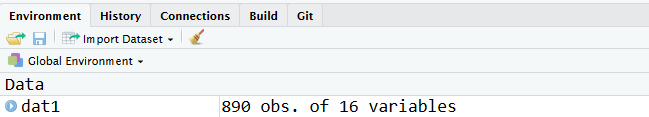
\includegraphics{images/str1.png}

The Rstudio IDE has a ton of really useful features that makes programming in R easier. Using the \texttt{View()} function within Rstudio will cause a new tab to open in the source panel with a view of your data. Hovering over the name of a column will cause the type of column to display. Any label attributes will be displayed in the view, and all columns in the view can be sorted.

\begin{Shaded}
\begin{Highlighting}[]
\OperatorTok{>}\StringTok{ }\KeywordTok{View}\NormalTok{(dat1)}
\end{Highlighting}
\end{Shaded}

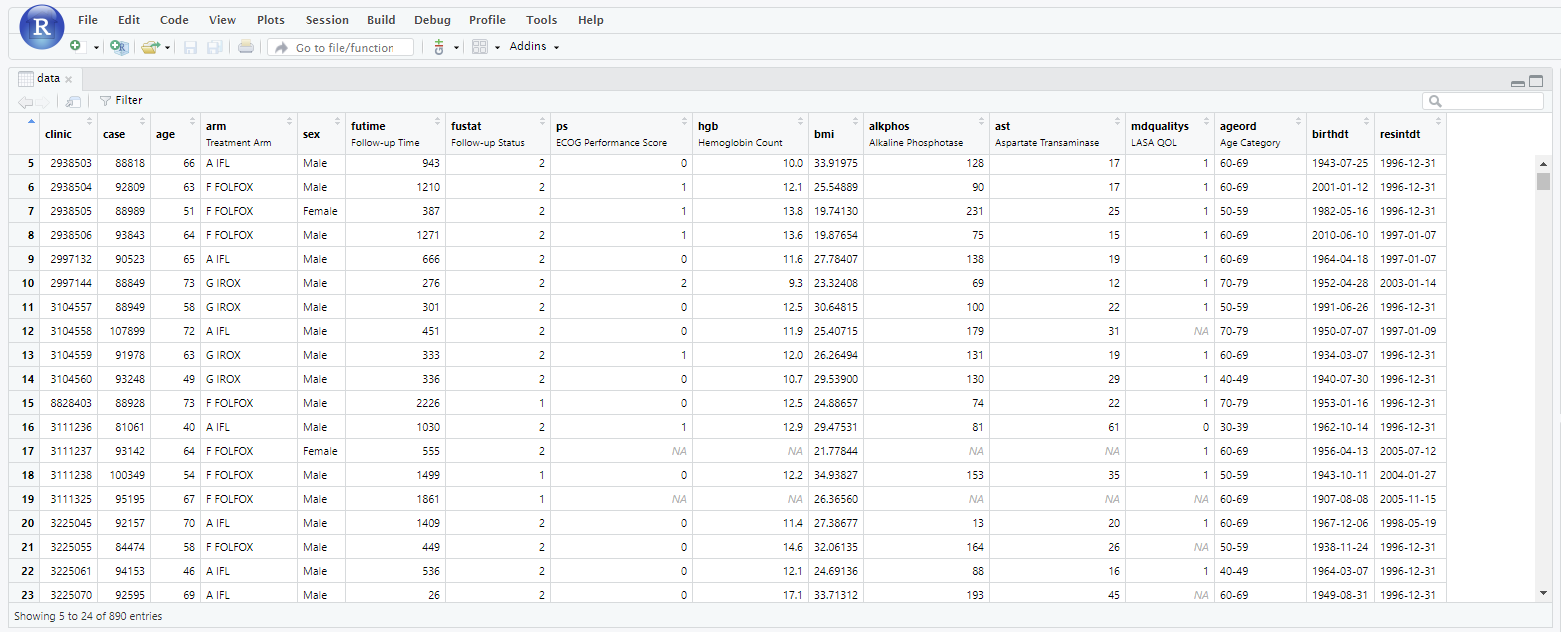
\includegraphics{images/View_data.png}

Here is some simple code that prints out the variable names and their classes using the functions \texttt{sapply()} and \texttt{class()}. \href{https://www.rdocumentation.org/packages/base/versions/current/topics/lapply}{sapply} is a function that looks at each element within a list (here, each variable) and runs the specified function (here, \texttt{class()}). Results are returned as a vector. Then, the \texttt{knitr} package includes the \texttt{kable} function which makes pretty default tables, especially for reports.
In the output below, the \texttt{class()} function is returning the class of each variable. Typical R classes for variables in a dataset include: character, numeric, integer, Date, logical, factor. More information on classes and data types can be found in Hadley Wickham's book \href{https://adv-r.hadley.nz/base-types.html}{Advanced R}.

\begin{Shaded}
\begin{Highlighting}[]
\OperatorTok{>}\StringTok{ }\KeywordTok{library}\NormalTok{(knitr)}
\OperatorTok{>}\StringTok{ }\KeywordTok{kable}\NormalTok{(}\KeywordTok{data.frame}\NormalTok{(}\DataTypeTok{Type =} \KeywordTok{sapply}\NormalTok{(}\DataTypeTok{X =}\NormalTok{ dat1, }\DataTypeTok{FUN =}\NormalTok{ class)))}
\end{Highlighting}
\end{Shaded}

\begin{tabular}{l|l}
\hline
  & Type\\
\hline
id & numeric\\
\hline
age & numeric\\
\hline
arm & character\\
\hline
sex & character\\
\hline
futime & numeric\\
\hline
fustat & numeric\\
\hline
ps & numeric\\
\hline
hgb & numeric\\
\hline
bmi & numeric\\
\hline
alkphos & numeric\\
\hline
ast & numeric\\
\hline
mdqualitys & numeric\\
\hline
ageord & character\\
\hline
birthdt & Date\\
\hline
resintdt & Date\\
\hline
\end{tabular}

Other options to this exercise can be found at the \protect\hyperlink{alt-import}{end of this document}.

\hypertarget{data-exploring}{%
\subsection{Data Exploring}\label{data-exploring}}

\begin{itemize}
\tightlist
\item
  \textbf{Take a closer look at the data using basic summary statistics. Do you notice any strange values? If so, fix them.}
\end{itemize}

There are a number of different tools that are available to explore a new dataset. The package \texttt{summarytools} includes the function \texttt{dfSummary()} which provides basic summaries of all of the variables in a dataset. When the summary is written directly to a file, it also provides nice graphical summaries of each variable.

\begin{Shaded}
\begin{Highlighting}[]
\OperatorTok{>}\StringTok{ }\KeywordTok{library}\NormalTok{(summarytools)}
\NormalTok{Registered S3 method overwritten by }\StringTok{'pryr'}\OperatorTok{:}
\StringTok{  }\NormalTok{method      from}
\NormalTok{  print.bytes Rcpp}
\NormalTok{Warning }\ControlFlowTok{in} \KeywordTok{fun}\NormalTok{(libname, pkgname)}\OperatorTok{:}\StringTok{ }\NormalTok{couldn}\StringTok{'t connect to display ":0"}
\StringTok{system might not have X11 capabilities; in case of errors when using dfSummary(), set st_options(use.x11 = FALSE)}

\StringTok{Attaching package: '}\NormalTok{summarytools}\StringTok{'}
\StringTok{The following object is masked from '}\NormalTok{package}\OperatorTok{:}\NormalTok{tibble}\StringTok{':}

\StringTok{    view}
\StringTok{> }
\StringTok{> # Settings to work well in markdown document (try running default settings}
\StringTok{> # interactively)}
\StringTok{> dfSummary(dat1, plain.ascii = FALSE, style = "grid", graph.col = FALSE, headings = TRUE)}
\end{Highlighting}
\end{Shaded}

\hypertarget{data-frame-summary}{%
\subsection{Data Frame Summary}\label{data-frame-summary}}

\hypertarget{dat1}{%
\subsubsection{dat1}\label{dat1}}

\textbf{Dimensions:} 890 x 15\\
\textbf{Duplicates:} 0

\begin{longtable}[]{@{}lllllll@{}}
\toprule
\begin{minipage}[b]{0.03\columnwidth}\raggedright
No\strut
\end{minipage} & \begin{minipage}[b]{0.09\columnwidth}\raggedright
Variable\strut
\end{minipage} & \begin{minipage}[b]{0.17\columnwidth}\raggedright
Label\strut
\end{minipage} & \begin{minipage}[b]{0.22\columnwidth}\raggedright
Stats / Values\strut
\end{minipage} & \begin{minipage}[b]{0.15\columnwidth}\raggedright
Freqs (\% of Valid)\strut
\end{minipage} & \begin{minipage}[b]{0.07\columnwidth}\raggedright
Valid\strut
\end{minipage} & \begin{minipage}[b]{0.07\columnwidth}\raggedright
Missing\strut
\end{minipage}\tabularnewline
\midrule
\endhead
\begin{minipage}[t]{0.03\columnwidth}\raggedright
1\strut
\end{minipage} & \begin{minipage}[t]{0.09\columnwidth}\raggedright
id\\
{[}numeric{]}\strut
\end{minipage} & \begin{minipage}[t]{0.17\columnwidth}\raggedright
\strut
\end{minipage} & \begin{minipage}[t]{0.22\columnwidth}\raggedright
Mean (sd) : 91495.3 (5017.7)\\
min \textless{} med \textless{} max:\\
76170 \textless{} 91912.5 \textless{} 112263\\
IQR (CV) : 4245 (0.1)\strut
\end{minipage} & \begin{minipage}[t]{0.15\columnwidth}\raggedright
889 distinct values\strut
\end{minipage} & \begin{minipage}[t]{0.07\columnwidth}\raggedright
890\\
(100\%)\strut
\end{minipage} & \begin{minipage}[t]{0.07\columnwidth}\raggedright
0\\
(0\%)\strut
\end{minipage}\tabularnewline
\begin{minipage}[t]{0.03\columnwidth}\raggedright
2\strut
\end{minipage} & \begin{minipage}[t]{0.09\columnwidth}\raggedright
age\\
{[}numeric{]}\strut
\end{minipage} & \begin{minipage}[t]{0.17\columnwidth}\raggedright
\strut
\end{minipage} & \begin{minipage}[t]{0.22\columnwidth}\raggedright
Mean (sd) : 60.2 (11.3)\\
min \textless{} med \textless{} max:\\
27 \textless{} 61 \textless{} 88\\
IQR (CV) : 16 (0.2)\strut
\end{minipage} & \begin{minipage}[t]{0.15\columnwidth}\raggedright
59 distinct values\strut
\end{minipage} & \begin{minipage}[t]{0.07\columnwidth}\raggedright
890\\
(100\%)\strut
\end{minipage} & \begin{minipage}[t]{0.07\columnwidth}\raggedright
0\\
(0\%)\strut
\end{minipage}\tabularnewline
\begin{minipage}[t]{0.03\columnwidth}\raggedright
3\strut
\end{minipage} & \begin{minipage}[t]{0.09\columnwidth}\raggedright
arm\\
{[}character{]}\strut
\end{minipage} & \begin{minipage}[t]{0.17\columnwidth}\raggedright
Treatment Arm\strut
\end{minipage} & \begin{minipage}[t]{0.22\columnwidth}\raggedright
1. A IFL\\
2. F FOLFOX\\
3. G IROX\strut
\end{minipage} & \begin{minipage}[t]{0.15\columnwidth}\raggedright
303 (34.0\%)\\
299 (33.6\%)\\
288 (32.4\%)\strut
\end{minipage} & \begin{minipage}[t]{0.07\columnwidth}\raggedright
890\\
(100\%)\strut
\end{minipage} & \begin{minipage}[t]{0.07\columnwidth}\raggedright
0\\
(0\%)\strut
\end{minipage}\tabularnewline
\begin{minipage}[t]{0.03\columnwidth}\raggedright
4\strut
\end{minipage} & \begin{minipage}[t]{0.09\columnwidth}\raggedright
sex\\
{[}character{]}\strut
\end{minipage} & \begin{minipage}[t]{0.17\columnwidth}\raggedright
\strut
\end{minipage} & \begin{minipage}[t]{0.22\columnwidth}\raggedright
1. 2\\
2. F\\
3. Female\\
4. Male\strut
\end{minipage} & \begin{minipage}[t]{0.15\columnwidth}\raggedright
2 ( 0.2\%)\\
2 ( 0.2\%)\\
347 (39.0\%)\\
539 (60.6\%)\strut
\end{minipage} & \begin{minipage}[t]{0.07\columnwidth}\raggedright
890\\
(100\%)\strut
\end{minipage} & \begin{minipage}[t]{0.07\columnwidth}\raggedright
0\\
(0\%)\strut
\end{minipage}\tabularnewline
\begin{minipage}[t]{0.03\columnwidth}\raggedright
5\strut
\end{minipage} & \begin{minipage}[t]{0.09\columnwidth}\raggedright
futime\\
{[}numeric{]}\strut
\end{minipage} & \begin{minipage}[t]{0.17\columnwidth}\raggedright
Follow-up Time\strut
\end{minipage} & \begin{minipage}[t]{0.22\columnwidth}\raggedright
Mean (sd) : 635.3 (487.8)\\
min \textless{} med \textless{} max:\\
9 \textless{} 516.5 \textless{} 2472\\
IQR (CV) : 546.2 (0.8)\strut
\end{minipage} & \begin{minipage}[t]{0.15\columnwidth}\raggedright
666 distinct values\strut
\end{minipage} & \begin{minipage}[t]{0.07\columnwidth}\raggedright
890\\
(100\%)\strut
\end{minipage} & \begin{minipage}[t]{0.07\columnwidth}\raggedright
0\\
(0\%)\strut
\end{minipage}\tabularnewline
\begin{minipage}[t]{0.03\columnwidth}\raggedright
6\strut
\end{minipage} & \begin{minipage}[t]{0.09\columnwidth}\raggedright
fustat\\
{[}numeric{]}\strut
\end{minipage} & \begin{minipage}[t]{0.17\columnwidth}\raggedright
Follow-up Status\strut
\end{minipage} & \begin{minipage}[t]{0.22\columnwidth}\raggedright
Min : 1\\
Mean : 1.9\\
Max : 2\strut
\end{minipage} & \begin{minipage}[t]{0.15\columnwidth}\raggedright
1 : 68 ( 7.6\%)\\
2 : 822 (92.4\%)\strut
\end{minipage} & \begin{minipage}[t]{0.07\columnwidth}\raggedright
890\\
(100\%)\strut
\end{minipage} & \begin{minipage}[t]{0.07\columnwidth}\raggedright
0\\
(0\%)\strut
\end{minipage}\tabularnewline
\begin{minipage}[t]{0.03\columnwidth}\raggedright
7\strut
\end{minipage} & \begin{minipage}[t]{0.09\columnwidth}\raggedright
ps\\
{[}numeric{]}\strut
\end{minipage} & \begin{minipage}[t]{0.17\columnwidth}\raggedright
ECOG Performance Score\strut
\end{minipage} & \begin{minipage}[t]{0.22\columnwidth}\raggedright
Mean (sd) : 0.5 (0.6)\\
min \textless{} med \textless{} max:\\
0 \textless{} 0 \textless{} 2\\
IQR (CV) : 1 (1.1)\strut
\end{minipage} & \begin{minipage}[t]{0.15\columnwidth}\raggedright
0 : 403 (52.3\%)\\
1 : 324 (42.1\%)\\
2 : 43 ( 5.6\%)\strut
\end{minipage} & \begin{minipage}[t]{0.07\columnwidth}\raggedright
770\\
(86.52\%)\strut
\end{minipage} & \begin{minipage}[t]{0.07\columnwidth}\raggedright
120\\
(13.48\%)\strut
\end{minipage}\tabularnewline
\begin{minipage}[t]{0.03\columnwidth}\raggedright
8\strut
\end{minipage} & \begin{minipage}[t]{0.09\columnwidth}\raggedright
hgb\\
{[}numeric{]}\strut
\end{minipage} & \begin{minipage}[t]{0.17\columnwidth}\raggedright
Hemoglobin Count\strut
\end{minipage} & \begin{minipage}[t]{0.22\columnwidth}\raggedright
Mean (sd) : 12.4 (1.7)\\
min \textless{} med \textless{} max:\\
9 \textless{} 12.2 \textless{} 18.2\\
IQR (CV) : 2.5 (0.1)\strut
\end{minipage} & \begin{minipage}[t]{0.15\columnwidth}\raggedright
84 distinct values\strut
\end{minipage} & \begin{minipage}[t]{0.07\columnwidth}\raggedright
770\\
(86.52\%)\strut
\end{minipage} & \begin{minipage}[t]{0.07\columnwidth}\raggedright
120\\
(13.48\%)\strut
\end{minipage}\tabularnewline
\begin{minipage}[t]{0.03\columnwidth}\raggedright
9\strut
\end{minipage} & \begin{minipage}[t]{0.09\columnwidth}\raggedright
bmi\\
{[}numeric{]}\strut
\end{minipage} & \begin{minipage}[t]{0.17\columnwidth}\raggedright
\strut
\end{minipage} & \begin{minipage}[t]{0.22\columnwidth}\raggedright
Mean (sd) : 27.1 (5.6)\\
min \textless{} med \textless{} max:\\
3.1 \textless{} 26.3 \textless{} 60.2\\
IQR (CV) : 6.3 (0.2)\strut
\end{minipage} & \begin{minipage}[t]{0.15\columnwidth}\raggedright
828 distinct values\strut
\end{minipage} & \begin{minipage}[t]{0.07\columnwidth}\raggedright
871\\
(97.87\%)\strut
\end{minipage} & \begin{minipage}[t]{0.07\columnwidth}\raggedright
19\\
(2.13\%)\strut
\end{minipage}\tabularnewline
\begin{minipage}[t]{0.03\columnwidth}\raggedright
10\strut
\end{minipage} & \begin{minipage}[t]{0.09\columnwidth}\raggedright
alkphos\\
{[}numeric{]}\strut
\end{minipage} & \begin{minipage}[t]{0.17\columnwidth}\raggedright
Alkaline Phosphotase\strut
\end{minipage} & \begin{minipage}[t]{0.22\columnwidth}\raggedright
Mean (sd) : 173.8 (135.7)\\
min \textless{} med \textless{} max:\\
7 \textless{} 125 \textless{} 1014\\
IQR (CV) : 126.8 (0.8)\strut
\end{minipage} & \begin{minipage}[t]{0.15\columnwidth}\raggedright
307 distinct values\strut
\end{minipage} & \begin{minipage}[t]{0.07\columnwidth}\raggedright
770\\
(86.52\%)\strut
\end{minipage} & \begin{minipage}[t]{0.07\columnwidth}\raggedright
120\\
(13.48\%)\strut
\end{minipage}\tabularnewline
\begin{minipage}[t]{0.03\columnwidth}\raggedright
11\strut
\end{minipage} & \begin{minipage}[t]{0.09\columnwidth}\raggedright
ast\\
{[}numeric{]}\strut
\end{minipage} & \begin{minipage}[t]{0.17\columnwidth}\raggedright
Aspartate Transaminase\strut
\end{minipage} & \begin{minipage}[t]{0.22\columnwidth}\raggedright
Mean (sd) : 36.5 (27.1)\\
min \textless{} med \textless{} max:\\
7 \textless{} 27 \textless{} 205\\
IQR (CV) : 22.8 (0.7)\strut
\end{minipage} & \begin{minipage}[t]{0.15\columnwidth}\raggedright
114 distinct values\strut
\end{minipage} & \begin{minipage}[t]{0.07\columnwidth}\raggedright
770\\
(86.52\%)\strut
\end{minipage} & \begin{minipage}[t]{0.07\columnwidth}\raggedright
120\\
(13.48\%)\strut
\end{minipage}\tabularnewline
\begin{minipage}[t]{0.03\columnwidth}\raggedright
12\strut
\end{minipage} & \begin{minipage}[t]{0.09\columnwidth}\raggedright
mdqualitys\\
{[}numeric{]}\strut
\end{minipage} & \begin{minipage}[t]{0.17\columnwidth}\raggedright
LASA QOL\strut
\end{minipage} & \begin{minipage}[t]{0.22\columnwidth}\raggedright
Min : 0\\
Mean : 0.9\\
Max : 1\strut
\end{minipage} & \begin{minipage}[t]{0.15\columnwidth}\raggedright
0 : 85 (10.7\%)\\
1 : 707 (89.3\%)\strut
\end{minipage} & \begin{minipage}[t]{0.07\columnwidth}\raggedright
792\\
(88.99\%)\strut
\end{minipage} & \begin{minipage}[t]{0.07\columnwidth}\raggedright
98\\
(11.01\%)\strut
\end{minipage}\tabularnewline
\begin{minipage}[t]{0.03\columnwidth}\raggedright
13\strut
\end{minipage} & \begin{minipage}[t]{0.09\columnwidth}\raggedright
ageord\\
{[}character{]}\strut
\end{minipage} & \begin{minipage}[t]{0.17\columnwidth}\raggedright
Age Category\strut
\end{minipage} & \begin{minipage}[t]{0.22\columnwidth}\raggedright
1. 20-29\\
2. 30-39\\
3. 40-49\\
4. 50-59\\
5. 60-69\\
6. 70-79\\
7. 80-89\strut
\end{minipage} & \begin{minipage}[t]{0.15\columnwidth}\raggedright
12 ( 1.4\%)\\
40 ( 4.5\%)\\
117 (13.2\%)\\
256 (28.8\%)\\
288 (32.4\%)\\
162 (18.2\%)\\
15 ( 1.7\%)\strut
\end{minipage} & \begin{minipage}[t]{0.07\columnwidth}\raggedright
890\\
(100\%)\strut
\end{minipage} & \begin{minipage}[t]{0.07\columnwidth}\raggedright
0\\
(0\%)\strut
\end{minipage}\tabularnewline
\begin{minipage}[t]{0.03\columnwidth}\raggedright
14\strut
\end{minipage} & \begin{minipage}[t]{0.09\columnwidth}\raggedright
birthdt\\
{[}Date{]}\strut
\end{minipage} & \begin{minipage}[t]{0.17\columnwidth}\raggedright
\strut
\end{minipage} & \begin{minipage}[t]{0.22\columnwidth}\raggedright
min : 1850-01-01\\
med : 1966-09-22\\
max : 2015-04-06\\
range : 165y 3m 5d\strut
\end{minipage} & \begin{minipage}[t]{0.15\columnwidth}\raggedright
638 distinct values\strut
\end{minipage} & \begin{minipage}[t]{0.07\columnwidth}\raggedright
890\\
(100\%)\strut
\end{minipage} & \begin{minipage}[t]{0.07\columnwidth}\raggedright
0\\
(0\%)\strut
\end{minipage}\tabularnewline
\begin{minipage}[t]{0.03\columnwidth}\raggedright
15\strut
\end{minipage} & \begin{minipage}[t]{0.09\columnwidth}\raggedright
resintdt\\
{[}Date{]}\strut
\end{minipage} & \begin{minipage}[t]{0.17\columnwidth}\raggedright
\strut
\end{minipage} & \begin{minipage}[t]{0.22\columnwidth}\raggedright
min : 1996-12-31\\
med : 1997-01-01\\
max : 2014-02-19\\
range : 17y 1m 19d\strut
\end{minipage} & \begin{minipage}[t]{0.15\columnwidth}\raggedright
50 distinct values\strut
\end{minipage} & \begin{minipage}[t]{0.07\columnwidth}\raggedright
812\\
(91.24\%)\strut
\end{minipage} & \begin{minipage}[t]{0.07\columnwidth}\raggedright
78\\
(8.76\%)\strut
\end{minipage}\tabularnewline
\bottomrule
\end{longtable}

\begin{Shaded}
\begin{Highlighting}[]
\OperatorTok{>}\StringTok{ }
\ErrorTok{>}\StringTok{ }\CommentTok{# Save the results to an external file (includes plots!)}
\ErrorTok{>}\StringTok{ }\KeywordTok{print}\NormalTok{(}\KeywordTok{dfSummary}\NormalTok{(dat1), }\DataTypeTok{file =} \StringTok{"dat1.html"}\NormalTok{)}
\NormalTok{Warning }\ControlFlowTok{in} \KeywordTok{png}\NormalTok{(png_loc <-}\StringTok{ }\KeywordTok{tempfile}\NormalTok{(}\DataTypeTok{fileext =} \StringTok{".png"}\NormalTok{), }\DataTypeTok{width =} \DecValTok{150} \OperatorTok{*}
\NormalTok{graph.magnif, }\OperatorTok{:}\StringTok{ }\NormalTok{unable to open connection to X11 display }\StringTok{''}
\NormalTok{Warning }\ControlFlowTok{in} \KeywordTok{png}\NormalTok{(png_loc <-}\StringTok{ }\KeywordTok{tempfile}\NormalTok{(}\DataTypeTok{fileext =} \StringTok{".png"}\NormalTok{), }\DataTypeTok{width =} \DecValTok{150} \OperatorTok{*}
\NormalTok{graph.magnif, }\OperatorTok{:}\StringTok{ }\NormalTok{unable to open connection to X11 display }\StringTok{''}
\NormalTok{Warning }\ControlFlowTok{in} \KeywordTok{png}\NormalTok{(png_loc <-}\StringTok{ }\KeywordTok{tempfile}\NormalTok{(}\DataTypeTok{fileext =} \StringTok{".png"}\NormalTok{), }\DataTypeTok{width =} \DecValTok{150} \OperatorTok{*}
\NormalTok{graph.magnif, }\OperatorTok{:}\StringTok{ }\NormalTok{unable to open connection to X11 display }\StringTok{''}

\NormalTok{Warning }\ControlFlowTok{in} \KeywordTok{png}\NormalTok{(png_loc <-}\StringTok{ }\KeywordTok{tempfile}\NormalTok{(}\DataTypeTok{fileext =} \StringTok{".png"}\NormalTok{), }\DataTypeTok{width =} \DecValTok{150} \OperatorTok{*}
\NormalTok{graph.magnif, }\OperatorTok{:}\StringTok{ }\NormalTok{unable to open connection to X11 display }\StringTok{''}
\NormalTok{Warning }\ControlFlowTok{in} \KeywordTok{png}\NormalTok{(png_loc <-}\StringTok{ }\KeywordTok{tempfile}\NormalTok{(}\DataTypeTok{fileext =} \StringTok{".png"}\NormalTok{), }\DataTypeTok{width =} \DecValTok{150} \OperatorTok{*}
\NormalTok{graph.magnif, }\OperatorTok{:}\StringTok{ }\NormalTok{unable to open connection to X11 display }\StringTok{''}
\NormalTok{Warning }\ControlFlowTok{in} \KeywordTok{png}\NormalTok{(png_loc <-}\StringTok{ }\KeywordTok{tempfile}\NormalTok{(}\DataTypeTok{fileext =} \StringTok{".png"}\NormalTok{), }\DataTypeTok{width =} \DecValTok{150} \OperatorTok{*}
\NormalTok{graph.magnif, }\OperatorTok{:}\StringTok{ }\NormalTok{unable to open connection to X11 display }\StringTok{''}

\NormalTok{Warning }\ControlFlowTok{in} \KeywordTok{png}\NormalTok{(png_loc <-}\StringTok{ }\KeywordTok{tempfile}\NormalTok{(}\DataTypeTok{fileext =} \StringTok{".png"}\NormalTok{), }\DataTypeTok{width =} \DecValTok{150} \OperatorTok{*}
\NormalTok{graph.magnif, }\OperatorTok{:}\StringTok{ }\NormalTok{unable to open connection to X11 display }\StringTok{''}
\NormalTok{Warning }\ControlFlowTok{in} \KeywordTok{png}\NormalTok{(png_loc <-}\StringTok{ }\KeywordTok{tempfile}\NormalTok{(}\DataTypeTok{fileext =} \StringTok{".png"}\NormalTok{), }\DataTypeTok{width =} \DecValTok{150} \OperatorTok{*}
\NormalTok{graph.magnif, }\OperatorTok{:}\StringTok{ }\NormalTok{unable to open connection to X11 display }\StringTok{''}

\NormalTok{Warning }\ControlFlowTok{in} \KeywordTok{png}\NormalTok{(png_loc <-}\StringTok{ }\KeywordTok{tempfile}\NormalTok{(}\DataTypeTok{fileext =} \StringTok{".png"}\NormalTok{), }\DataTypeTok{width =} \DecValTok{150} \OperatorTok{*}
\NormalTok{graph.magnif, }\OperatorTok{:}\StringTok{ }\NormalTok{unable to open connection to X11 display }\StringTok{''}

\NormalTok{Warning }\ControlFlowTok{in} \KeywordTok{png}\NormalTok{(png_loc <-}\StringTok{ }\KeywordTok{tempfile}\NormalTok{(}\DataTypeTok{fileext =} \StringTok{".png"}\NormalTok{), }\DataTypeTok{width =} \DecValTok{150} \OperatorTok{*}
\NormalTok{graph.magnif, }\OperatorTok{:}\StringTok{ }\NormalTok{unable to open connection to X11 display }\StringTok{''}

\NormalTok{Warning }\ControlFlowTok{in} \KeywordTok{png}\NormalTok{(png_loc <-}\StringTok{ }\KeywordTok{tempfile}\NormalTok{(}\DataTypeTok{fileext =} \StringTok{".png"}\NormalTok{), }\DataTypeTok{width =} \DecValTok{150} \OperatorTok{*}
\NormalTok{graph.magnif, }\OperatorTok{:}\StringTok{ }\NormalTok{unable to open connection to X11 display }\StringTok{''}
\NormalTok{Warning }\ControlFlowTok{in} \KeywordTok{png}\NormalTok{(png_loc <-}\StringTok{ }\KeywordTok{tempfile}\NormalTok{(}\DataTypeTok{fileext =} \StringTok{".png"}\NormalTok{), }\DataTypeTok{width =} \DecValTok{150} \OperatorTok{*}
\NormalTok{graph.magnif, }\OperatorTok{:}\StringTok{ }\NormalTok{unable to open connection to X11 display }\StringTok{''}

\NormalTok{Warning }\ControlFlowTok{in} \KeywordTok{png}\NormalTok{(png_loc <-}\StringTok{ }\KeywordTok{tempfile}\NormalTok{(}\DataTypeTok{fileext =} \StringTok{".png"}\NormalTok{), }\DataTypeTok{width =} \DecValTok{150} \OperatorTok{*}
\NormalTok{graph.magnif, }\OperatorTok{:}\StringTok{ }\NormalTok{unable to open connection to X11 display }\StringTok{''}
\NormalTok{Warning }\ControlFlowTok{in} \KeywordTok{png}\NormalTok{(png_loc <-}\StringTok{ }\KeywordTok{tempfile}\NormalTok{(}\DataTypeTok{fileext =} \StringTok{".png"}\NormalTok{), }\DataTypeTok{width =} \DecValTok{150} \OperatorTok{*}
\NormalTok{graph.magnif, }\OperatorTok{:}\StringTok{ }\NormalTok{unable to open connection to X11 display }\StringTok{''}

\NormalTok{Warning }\ControlFlowTok{in} \KeywordTok{png}\NormalTok{(png_loc <-}\StringTok{ }\KeywordTok{tempfile}\NormalTok{(}\DataTypeTok{fileext =} \StringTok{".png"}\NormalTok{), }\DataTypeTok{width =} \DecValTok{150} \OperatorTok{*}
\NormalTok{graph.magnif, }\OperatorTok{:}\StringTok{ }\NormalTok{unable to open connection to X11 display }\StringTok{''}
\NormalTok{Switching method to }\StringTok{'browser'}
\NormalTok{Output file written}\OperatorTok{:}\StringTok{ }\ErrorTok{/}\NormalTok{home}\OperatorTok{/}\NormalTok{atkinson}\OperatorTok{/}\NormalTok{education}\OperatorTok{/}\NormalTok{R_project_recipes}\OperatorTok{/}\NormalTok{dat1.html}
\end{Highlighting}
\end{Shaded}

See the \href{dat1.html}{external file version}.

Another option is to use the \texttt{tableby()} function that is available in the Mayo package \texttt{arsenal}. Tableby is a fantastic function for quick summaries for data exploration or reporting ``table 1'' describing the cohort. This function allows you to summarize the data stratified by some ``by'' variable or overall without any stratification. The code \texttt{\textasciitilde{}\ sex\ +\ arm\ +\ age\ +\ bmi} is a formula. If you wanted to stratify by a variable you would list the stratification variable on the left hand side of the \texttt{\textasciitilde{}}. The \texttt{tableby} function does all the calculations, but it doesn't create the information in a nice format. The \texttt{summary()} function pulls everything together into a nice table. Note that when you type \texttt{summary} here you are actually using \texttt{summary.tableby()}. This is important when looking for help with summarizing the \texttt{tableby} output.

If you want to look at the summary in your console window, you might want to use \texttt{summary(tab1,\ text=T)}. In order for the table to look nice within an R markdown (knitr) report, you just need to specify
\texttt{results="asis"} when creating the r chunk. This changes the layout slightly (compresses it) and bolds the variable names.

\begin{Shaded}
\begin{Highlighting}[]
\OperatorTok{>}\StringTok{ }\KeywordTok{library}\NormalTok{(arsenal)}
\OperatorTok{>}\StringTok{ }\NormalTok{tab1 <-}\StringTok{ }\KeywordTok{tableby}\NormalTok{(}\OperatorTok{~}\NormalTok{sex }\OperatorTok{+}\StringTok{ }\NormalTok{arm }\OperatorTok{+}\StringTok{ }\NormalTok{age }\OperatorTok{+}\StringTok{ }\NormalTok{bmi, }\DataTypeTok{data =}\NormalTok{ dat1)}
\OperatorTok{>}\StringTok{ }\KeywordTok{class}\NormalTok{(tab1)}
\end{Highlighting}
\end{Shaded}

{[}1{]} ``tableby'' ``arsenal\_table''

\begin{Shaded}
\begin{Highlighting}[]
\OperatorTok{>}\StringTok{ }\KeywordTok{summary}\NormalTok{(tab1, }\DataTypeTok{title =} \StringTok{"Baseline and patient characteristics"}\NormalTok{)}
\end{Highlighting}
\end{Shaded}

\begin{longtable}[]{@{}lc@{}}
\caption{Baseline and patient characteristics}\tabularnewline
\toprule
& Overall (N=890)\tabularnewline
\midrule
\endfirsthead
\toprule
& Overall (N=890)\tabularnewline
\midrule
\endhead
\textbf{sex} &\tabularnewline
~~~2 & 2 (0.2\%)\tabularnewline
~~~F & 2 (0.2\%)\tabularnewline
~~~Female & 347 (39.0\%)\tabularnewline
~~~Male & 539 (60.6\%)\tabularnewline
\textbf{Treatment Arm} &\tabularnewline
~~~A IFL & 303 (34.0\%)\tabularnewline
~~~F FOLFOX & 299 (33.6\%)\tabularnewline
~~~G IROX & 288 (32.4\%)\tabularnewline
\textbf{age} &\tabularnewline
~~~Mean (SD) & 60.152 (11.342)\tabularnewline
~~~Range & 27.000 - 88.000\tabularnewline
\textbf{bmi} &\tabularnewline
~~~N-Miss & 19\tabularnewline
~~~Mean (SD) & 27.106 (5.620)\tabularnewline
~~~Range & 3.060 - 60.243\tabularnewline
\bottomrule
\end{longtable}

If you want to examine every variable in \texttt{dat} you can use the shortcut \texttt{.}.

\begin{Shaded}
\begin{Highlighting}[]
\OperatorTok{>}\StringTok{ }\NormalTok{tab1 <-}\StringTok{ }\KeywordTok{tableby}\NormalTok{(}\OperatorTok{~}\NormalTok{., }\DataTypeTok{data =}\NormalTok{ dat1)}
\end{Highlighting}
\end{Shaded}

Based on these summaries, it appears that \texttt{sex} was not coded correctly and needs to be fixed. Our investigator confirms that \texttt{2} is supposed to be female. To correct this, we will pull out all the values in the variable sex within the \texttt{dat1} dataset that are equal to 2 or F (\texttt{dat1\$sex{[}dat1\$sex\ \%in\%\ c(\textquotesingle{}2\textquotesingle{},\textquotesingle{}F\textquotesingle{}){]}}) and assign those values to be equal to ``Female'' (\texttt{\textless{}-\ \textquotesingle{}Female\textquotesingle{}}).

\begin{Shaded}
\begin{Highlighting}[]
\OperatorTok{>}\StringTok{ }\KeywordTok{table}\NormalTok{(dat1}\OperatorTok{$}\NormalTok{sex)}

     \DecValTok{2}\NormalTok{      F Female   Male }
     \DecValTok{2}      \DecValTok{2}    \DecValTok{347}    \DecValTok{539} 
\OperatorTok{>}\StringTok{ }
\ErrorTok{>}\StringTok{ }\CommentTok{# For those observations that are 2 or F, change them to Female}
\ErrorTok{>}\StringTok{ }\NormalTok{dat1}\OperatorTok{$}\NormalTok{sex[dat1}\OperatorTok{$}\NormalTok{sex }\OperatorTok\StringTok{ }\KeywordTok{c}\NormalTok{(}\StringTok{"2"}\NormalTok{, }\StringTok{"F"}\NormalTok{)] <-}\StringTok{ "Female"}
\OperatorTok{>}\StringTok{ }
\ErrorTok{>}\StringTok{ }\KeywordTok{table}\NormalTok{(dat1}\OperatorTok{$}\NormalTok{sex)}

\NormalTok{Female   Male }
   \DecValTok{351}    \DecValTok{539} 
\end{Highlighting}
\end{Shaded}

One of the tricky functions in R for SAS programmers is the \texttt{ifelse()} function which differs from \texttt{if()\ \{\}\ else\ \{\}}. Suppose that you believe that all observations over a certain cutoff are errors and you want to set them equal to missing. The code below uses \texttt{ifelse}. The first argument creates a logical True/False variable. For those observations where the ``test'' is TRUE, use the value in the ``yes'' field and for those observations where the ``test'' is FALSE, use the value in the ``no'' field.

\begin{Shaded}
\begin{Highlighting}[]
\OperatorTok{>}\StringTok{ }\NormalTok{ast <-}\StringTok{ }\NormalTok{dat1}\OperatorTok{$}\NormalTok{ast}
\OperatorTok{>}\StringTok{ }\KeywordTok{summary}\NormalTok{(ast)}
\NormalTok{   Min. 1st Qu.  Median    Mean 3rd Qu.    Max.    NA}\StringTok{'s }
\StringTok{   7.00   20.00   27.00   36.46   42.75  205.00     120 }
\StringTok{> ast2 <- ifelse(test = ast > 45, yes = NA, no = ast)}
\StringTok{> summary(ast2)}
\StringTok{   Min. 1st Qu.  Median    Mean 3rd Qu.    Max.    NA'}\NormalTok{s }
   \FloatTok{7.00}   \FloatTok{19.00}   \FloatTok{24.00}   \FloatTok{25.21}   \FloatTok{31.00}   \FloatTok{45.00}     \DecValTok{286} 
\end{Highlighting}
\end{Shaded}

If instead I was creating a loop and I had one logical value, then I would do something like the following using \texttt{if()\ else()}.

\begin{Shaded}
\begin{Highlighting}[]
\OperatorTok{>}\StringTok{ }\NormalTok{group <-}\StringTok{ "A IFL"}
\OperatorTok{>}\StringTok{ }
\ErrorTok{>}\StringTok{ }\ControlFlowTok{if}\NormalTok{ (group }\OperatorTok{==}\StringTok{ "A IFL"}\NormalTok{) \{}
\OperatorTok{+}\StringTok{     }\KeywordTok{summary}\NormalTok{(ast)}
\OperatorTok{+}\StringTok{ }\NormalTok{\} }\ControlFlowTok{else}\NormalTok{ \{}
\OperatorTok{+}\StringTok{     }\KeywordTok{summary}\NormalTok{(ast2)}
\OperatorTok{+}\StringTok{ }\NormalTok{\}}
\NormalTok{   Min. 1st Qu.  Median    Mean 3rd Qu.    Max.    NA}\StringTok{'s }
\StringTok{   7.00   20.00   27.00   36.46   42.75  205.00     120 }
\end{Highlighting}
\end{Shaded}

An alternative to \texttt{ifelse} is the \texttt{case\_when()} function in the \texttt{dplyr} package. It is particularly useful when you have multiple nested ``ifelse'' statements. For instance, this is another alternative for fixing the code for sex.

\begin{Shaded}
\begin{Highlighting}[]
\OperatorTok{>}\StringTok{ }\NormalTok{dat1}\OperatorTok{$}\NormalTok{sex <-}\StringTok{ }\KeywordTok{case_when}\NormalTok{(dat1}\OperatorTok{$}\NormalTok{sex }\OperatorTok{==}\StringTok{ }\DecValTok{2} \OperatorTok{~}\StringTok{ "Female"}\NormalTok{, dat1}\OperatorTok{$}\NormalTok{sex }\OperatorTok{==}\StringTok{ "F"} \OperatorTok{~}\StringTok{ "Female"}\NormalTok{, }\OtherTok{TRUE} \OperatorTok{~}\StringTok{ }
\OperatorTok{+}\StringTok{     }\NormalTok{dat1}\OperatorTok{$}\NormalTok{sex)}
\end{Highlighting}
\end{Shaded}

\begin{itemize}
\tightlist
\item
  \textbf{Oops, there is a duplicate observation in the data. Confirm the data is the same for all the variables and remove one of the duplicates.}
\end{itemize}

Mistakes in data entry occur all the time. It is wise to check for duplicate records and/or more than one record per unique patient. There are a few different tools that can be used to check for duplicate observations including the functions \texttt{duplicated()} and \texttt{dplyr::distinct()}.

\begin{Shaded}
\begin{Highlighting}[]
\OperatorTok{>}\StringTok{ }\CommentTok{# count how many times each id appears in dat1}
\ErrorTok{>}\StringTok{ }\KeywordTok{table}\NormalTok{(}\KeywordTok{table}\NormalTok{(dat1}\OperatorTok{$}\NormalTok{id))}

  \DecValTok{1}   \DecValTok{2} 
\DecValTok{888}   \DecValTok{1} 
\OperatorTok{>}\StringTok{ }
\ErrorTok{>}\StringTok{ }
\ErrorTok{>}\StringTok{ }\CommentTok{# This next line of code first identifies which ids are duplicated:}
\ErrorTok{>}\StringTok{ }\CommentTok{# 'duplicated(dat1$id)' Then, it selects those ids from 'dat1$id' and returns}
\ErrorTok{>}\StringTok{ }\CommentTok{# only one instance of each duplicated ids using 'unique()'.}
\ErrorTok{>}\StringTok{ }
\ErrorTok{>}\StringTok{ }\NormalTok{tmp <-}\StringTok{ }\KeywordTok{unique}\NormalTok{(dat1}\OperatorTok{$}\NormalTok{id[}\KeywordTok{duplicated}\NormalTok{(dat1}\OperatorTok{$}\NormalTok{id)])}
\OperatorTok{>}\StringTok{ }
\ErrorTok{>}\StringTok{ }\CommentTok{# which rows have a duplicate?}
\ErrorTok{>}\StringTok{ }\NormalTok{dup.rows <-}\StringTok{ }\KeywordTok{which}\NormalTok{(dat1}\OperatorTok{$}\NormalTok{id }\OperatorTok\StringTok{ }\NormalTok{tmp)}
\OperatorTok{>}\StringTok{ }
\ErrorTok{>}\StringTok{ }\CommentTok{# show a portion of the data with the duplicates - which version do you keep?}
\ErrorTok{>}\StringTok{ }\CommentTok{# the kable function is available in the knitr package}
\ErrorTok{>}\StringTok{ }\KeywordTok{kable}\NormalTok{(dat1[dup.rows, }\KeywordTok{c}\NormalTok{(}\StringTok{"id"}\NormalTok{, }\StringTok{"age"}\NormalTok{, }\StringTok{"arm"}\NormalTok{, }\StringTok{"sex"}\NormalTok{, }\StringTok{"bmi"}\NormalTok{)])}
\end{Highlighting}
\end{Shaded}

\begin{tabular}{r|r|l|l|r}
\hline
id & age & arm & sex & bmi\\
\hline
101106 & 79 & F FOLFOX & Female & 3.059935\\
\hline
101106 & 79 & F FOLFOX & Female & 30.599346\\
\hline
\end{tabular}

This same code can be run using the following \texttt{dplyr} commands. It also illustrates the use of ``piping'', which is what the 3 character string \texttt{\%\textgreater{}\%} is called. Basically, it allows you to combine a bunch of commands together without having to save out temporary datasets. The \texttt{filter} command keeps only those observations where the condition is true. The \texttt{select} function keeps only certain variables.

\begin{Shaded}
\begin{Highlighting}[]
\OperatorTok{>}\StringTok{ }\CommentTok{# Using dplyr code this would be}
\ErrorTok{>}\StringTok{ }\NormalTok{dat1 }\OperatorTok\StringTok{ }\KeywordTok{filter}\NormalTok{(id }\OperatorTok\StringTok{ }\NormalTok{tmp) }\OperatorTok\StringTok{ }\KeywordTok{select}\NormalTok{(id, age, arm, sex, bmi) }\OperatorTok\StringTok{ }\KeywordTok{kable}\NormalTok{()}
\end{Highlighting}
\end{Shaded}

\begin{tabular}{r|r|l|l|r}
\hline
id & age & arm & sex & bmi\\
\hline
101106 & 79 & F FOLFOX & Female & 3.059935\\
\hline
101106 & 79 & F FOLFOX & Female & 30.599346\\
\hline
\end{tabular}

Now check to see if the observations are a complete duplicate or not.

\begin{Shaded}
\begin{Highlighting}[]
\OperatorTok{>}\StringTok{ }\CommentTok{# When you use `duplicated()` on a data.frame, it will test for completely}
\ErrorTok{>}\StringTok{ }\CommentTok{# identical rows.}
\ErrorTok{>}\StringTok{ }\KeywordTok{table}\NormalTok{(}\KeywordTok{duplicated}\NormalTok{(dat1))}

\OtherTok{FALSE} 
  \DecValTok{890} 
\OperatorTok{>}\StringTok{ }
\ErrorTok{>}\StringTok{ }\CommentTok{# remove rows with duplicate values (2 different approaches) Both approaches will}
\ErrorTok{>}\StringTok{ }\CommentTok{# return the first instance of a row and will exclude any duplicated rows.  This}
\ErrorTok{>}\StringTok{ }\CommentTok{# is similar to `FIRST.` in SAS.}
\ErrorTok{>}\StringTok{ }\KeywordTok{dim}\NormalTok{(dat1)}
\NormalTok{[}\DecValTok{1}\NormalTok{] }\DecValTok{890}  \DecValTok{15}
\OperatorTok{>}\StringTok{ }
\ErrorTok{>}\StringTok{ }\NormalTok{dat2 <-}\StringTok{ }\NormalTok{dat1[}\OperatorTok{!}\KeywordTok{duplicated}\NormalTok{(dat1), ]}
\OperatorTok{>}\StringTok{ }\KeywordTok{dim}\NormalTok{(dat2)}
\NormalTok{[}\DecValTok{1}\NormalTok{] }\DecValTok{890}  \DecValTok{15}
\end{Highlighting}
\end{Shaded}

\begin{itemize}
\tightlist
\item
  \textbf{Summarize age, gender, bmi, \ldots{} by the treatment variable using parametric statistics}
\end{itemize}

Again, this is an instance where \texttt{tableby} produces a nice table. Here the variable \texttt{arm} is listed on the left-hand side of the formula. The option \texttt{pfootnote=TRUE} indicates that the summary table should show a footnote indicating what test was run.

\begin{Shaded}
\begin{Highlighting}[]
\OperatorTok{>}\StringTok{ }\NormalTok{tab1 <-}\StringTok{ }\KeywordTok{tableby}\NormalTok{(arm }\OperatorTok{~}\StringTok{ }\NormalTok{age }\OperatorTok{+}\StringTok{ }\NormalTok{sex }\OperatorTok{+}\StringTok{ }\NormalTok{ps }\OperatorTok{+}\StringTok{ }\NormalTok{bmi }\OperatorTok{+}\StringTok{ }\NormalTok{alkphos }\OperatorTok{+}\StringTok{ }\NormalTok{mdqualitys }\OperatorTok{+}\StringTok{ }\NormalTok{ageord }\OperatorTok{+}\StringTok{ }\NormalTok{birthdt, }
\OperatorTok{+}\StringTok{     }\DataTypeTok{data =}\NormalTok{ dat2)}
\OperatorTok{>}\StringTok{ }\KeywordTok{summary}\NormalTok{(tab1, }\DataTypeTok{pfootnote =} \OtherTok{TRUE}\NormalTok{, }\DataTypeTok{total =} \OtherTok{FALSE}\NormalTok{)}
\end{Highlighting}
\end{Shaded}

\begin{longtable}[]{@{}lcccr@{}}
\toprule
\begin{minipage}[b]{0.21\columnwidth}\raggedright
\strut
\end{minipage} & \begin{minipage}[b]{0.19\columnwidth}\centering
A IFL (N=303)\strut
\end{minipage} & \begin{minipage}[b]{0.19\columnwidth}\centering
F FOLFOX (N=299)\strut
\end{minipage} & \begin{minipage}[b]{0.19\columnwidth}\centering
G IROX (N=288)\strut
\end{minipage} & \begin{minipage}[b]{0.07\columnwidth}\raggedleft
p value\strut
\end{minipage}\tabularnewline
\midrule
\endhead
\begin{minipage}[t]{0.21\columnwidth}\raggedright
\textbf{age}\strut
\end{minipage} & \begin{minipage}[t]{0.19\columnwidth}\centering
\strut
\end{minipage} & \begin{minipage}[t]{0.19\columnwidth}\centering
\strut
\end{minipage} & \begin{minipage}[t]{0.19\columnwidth}\centering
\strut
\end{minipage} & \begin{minipage}[t]{0.07\columnwidth}\raggedleft
0.585\textsuperscript{1}\strut
\end{minipage}\tabularnewline
\begin{minipage}[t]{0.21\columnwidth}\raggedright
~~~Mean (SD)\strut
\end{minipage} & \begin{minipage}[t]{0.19\columnwidth}\centering
59.696 (11.365)\strut
\end{minipage} & \begin{minipage}[t]{0.19\columnwidth}\centering
60.652 (11.422)\strut
\end{minipage} & \begin{minipage}[t]{0.19\columnwidth}\centering
60.111 (11.253)\strut
\end{minipage} & \begin{minipage}[t]{0.07\columnwidth}\raggedleft
\strut
\end{minipage}\tabularnewline
\begin{minipage}[t]{0.21\columnwidth}\raggedright
~~~Range\strut
\end{minipage} & \begin{minipage}[t]{0.19\columnwidth}\centering
27.000 - 88.000\strut
\end{minipage} & \begin{minipage}[t]{0.19\columnwidth}\centering
27.000 - 88.000\strut
\end{minipage} & \begin{minipage}[t]{0.19\columnwidth}\centering
28.000 - 84.000\strut
\end{minipage} & \begin{minipage}[t]{0.07\columnwidth}\raggedleft
\strut
\end{minipage}\tabularnewline
\begin{minipage}[t]{0.21\columnwidth}\raggedright
\textbf{sex}\strut
\end{minipage} & \begin{minipage}[t]{0.19\columnwidth}\centering
\strut
\end{minipage} & \begin{minipage}[t]{0.19\columnwidth}\centering
\strut
\end{minipage} & \begin{minipage}[t]{0.19\columnwidth}\centering
\strut
\end{minipage} & \begin{minipage}[t]{0.07\columnwidth}\raggedleft
0.175\textsuperscript{2}\strut
\end{minipage}\tabularnewline
\begin{minipage}[t]{0.21\columnwidth}\raggedright
~~~Female\strut
\end{minipage} & \begin{minipage}[t]{0.19\columnwidth}\centering
107 (35.3\%)\strut
\end{minipage} & \begin{minipage}[t]{0.19\columnwidth}\centering
127 (42.5\%)\strut
\end{minipage} & \begin{minipage}[t]{0.19\columnwidth}\centering
117 (40.6\%)\strut
\end{minipage} & \begin{minipage}[t]{0.07\columnwidth}\raggedleft
\strut
\end{minipage}\tabularnewline
\begin{minipage}[t]{0.21\columnwidth}\raggedright
~~~Male\strut
\end{minipage} & \begin{minipage}[t]{0.19\columnwidth}\centering
196 (64.7\%)\strut
\end{minipage} & \begin{minipage}[t]{0.19\columnwidth}\centering
172 (57.5\%)\strut
\end{minipage} & \begin{minipage}[t]{0.19\columnwidth}\centering
171 (59.4\%)\strut
\end{minipage} & \begin{minipage}[t]{0.07\columnwidth}\raggedleft
\strut
\end{minipage}\tabularnewline
\begin{minipage}[t]{0.21\columnwidth}\raggedright
\textbf{ECOG Performance Score}\strut
\end{minipage} & \begin{minipage}[t]{0.19\columnwidth}\centering
\strut
\end{minipage} & \begin{minipage}[t]{0.19\columnwidth}\centering
\strut
\end{minipage} & \begin{minipage}[t]{0.19\columnwidth}\centering
\strut
\end{minipage} & \begin{minipage}[t]{0.07\columnwidth}\raggedleft
0.781\textsuperscript{1}\strut
\end{minipage}\tabularnewline
\begin{minipage}[t]{0.21\columnwidth}\raggedright
~~~N-Miss\strut
\end{minipage} & \begin{minipage}[t]{0.19\columnwidth}\centering
45\strut
\end{minipage} & \begin{minipage}[t]{0.19\columnwidth}\centering
39\strut
\end{minipage} & \begin{minipage}[t]{0.19\columnwidth}\centering
36\strut
\end{minipage} & \begin{minipage}[t]{0.07\columnwidth}\raggedleft
\strut
\end{minipage}\tabularnewline
\begin{minipage}[t]{0.21\columnwidth}\raggedright
~~~Mean (SD)\strut
\end{minipage} & \begin{minipage}[t]{0.19\columnwidth}\centering
0.512 (0.600)\strut
\end{minipage} & \begin{minipage}[t]{0.19\columnwidth}\centering
0.538 (0.598)\strut
\end{minipage} & \begin{minipage}[t]{0.19\columnwidth}\centering
0.548 (0.607)\strut
\end{minipage} & \begin{minipage}[t]{0.07\columnwidth}\raggedleft
\strut
\end{minipage}\tabularnewline
\begin{minipage}[t]{0.21\columnwidth}\raggedright
~~~Range\strut
\end{minipage} & \begin{minipage}[t]{0.19\columnwidth}\centering
0.000 - 2.000\strut
\end{minipage} & \begin{minipage}[t]{0.19\columnwidth}\centering
0.000 - 2.000\strut
\end{minipage} & \begin{minipage}[t]{0.19\columnwidth}\centering
0.000 - 2.000\strut
\end{minipage} & \begin{minipage}[t]{0.07\columnwidth}\raggedleft
\strut
\end{minipage}\tabularnewline
\begin{minipage}[t]{0.21\columnwidth}\raggedright
\textbf{bmi}\strut
\end{minipage} & \begin{minipage}[t]{0.19\columnwidth}\centering
\strut
\end{minipage} & \begin{minipage}[t]{0.19\columnwidth}\centering
\strut
\end{minipage} & \begin{minipage}[t]{0.19\columnwidth}\centering
\strut
\end{minipage} & \begin{minipage}[t]{0.07\columnwidth}\raggedleft
0.745\textsuperscript{1}\strut
\end{minipage}\tabularnewline
\begin{minipage}[t]{0.21\columnwidth}\raggedright
~~~N-Miss\strut
\end{minipage} & \begin{minipage}[t]{0.19\columnwidth}\centering
6\strut
\end{minipage} & \begin{minipage}[t]{0.19\columnwidth}\centering
9\strut
\end{minipage} & \begin{minipage}[t]{0.19\columnwidth}\centering
4\strut
\end{minipage} & \begin{minipage}[t]{0.07\columnwidth}\raggedleft
\strut
\end{minipage}\tabularnewline
\begin{minipage}[t]{0.21\columnwidth}\raggedright
~~~Mean (SD)\strut
\end{minipage} & \begin{minipage}[t]{0.19\columnwidth}\centering
27.278 (5.493)\strut
\end{minipage} & \begin{minipage}[t]{0.19\columnwidth}\centering
27.112 (5.499)\strut
\end{minipage} & \begin{minipage}[t]{0.19\columnwidth}\centering
26.920 (5.883)\strut
\end{minipage} & \begin{minipage}[t]{0.07\columnwidth}\raggedleft
\strut
\end{minipage}\tabularnewline
\begin{minipage}[t]{0.21\columnwidth}\raggedright
~~~Range\strut
\end{minipage} & \begin{minipage}[t]{0.19\columnwidth}\centering
14.053 - 53.008\strut
\end{minipage} & \begin{minipage}[t]{0.19\columnwidth}\centering
3.060 - 49.130\strut
\end{minipage} & \begin{minipage}[t]{0.19\columnwidth}\centering
16.071 - 60.243\strut
\end{minipage} & \begin{minipage}[t]{0.07\columnwidth}\raggedleft
\strut
\end{minipage}\tabularnewline
\begin{minipage}[t]{0.21\columnwidth}\raggedright
\textbf{Alkaline Phosphotase}\strut
\end{minipage} & \begin{minipage}[t]{0.19\columnwidth}\centering
\strut
\end{minipage} & \begin{minipage}[t]{0.19\columnwidth}\centering
\strut
\end{minipage} & \begin{minipage}[t]{0.19\columnwidth}\centering
\strut
\end{minipage} & \begin{minipage}[t]{0.07\columnwidth}\raggedleft
0.707\textsuperscript{1}\strut
\end{minipage}\tabularnewline
\begin{minipage}[t]{0.21\columnwidth}\raggedright
~~~N-Miss\strut
\end{minipage} & \begin{minipage}[t]{0.19\columnwidth}\centering
45\strut
\end{minipage} & \begin{minipage}[t]{0.19\columnwidth}\centering
39\strut
\end{minipage} & \begin{minipage}[t]{0.19\columnwidth}\centering
36\strut
\end{minipage} & \begin{minipage}[t]{0.07\columnwidth}\raggedleft
\strut
\end{minipage}\tabularnewline
\begin{minipage}[t]{0.21\columnwidth}\raggedright
~~~Mean (SD)\strut
\end{minipage} & \begin{minipage}[t]{0.19\columnwidth}\centering
170.612 (124.842)\strut
\end{minipage} & \begin{minipage}[t]{0.19\columnwidth}\centering
171.377 (133.671)\strut
\end{minipage} & \begin{minipage}[t]{0.19\columnwidth}\centering
179.663 (148.110)\strut
\end{minipage} & \begin{minipage}[t]{0.07\columnwidth}\raggedleft
\strut
\end{minipage}\tabularnewline
\begin{minipage}[t]{0.21\columnwidth}\raggedright
~~~Range\strut
\end{minipage} & \begin{minipage}[t]{0.19\columnwidth}\centering
13.000 - 858.000\strut
\end{minipage} & \begin{minipage}[t]{0.19\columnwidth}\centering
18.000 - 1014.000\strut
\end{minipage} & \begin{minipage}[t]{0.19\columnwidth}\centering
7.000 - 982.000\strut
\end{minipage} & \begin{minipage}[t]{0.07\columnwidth}\raggedleft
\strut
\end{minipage}\tabularnewline
\begin{minipage}[t]{0.21\columnwidth}\raggedright
\textbf{LASA QOL}\strut
\end{minipage} & \begin{minipage}[t]{0.19\columnwidth}\centering
\strut
\end{minipage} & \begin{minipage}[t]{0.19\columnwidth}\centering
\strut
\end{minipage} & \begin{minipage}[t]{0.19\columnwidth}\centering
\strut
\end{minipage} & \begin{minipage}[t]{0.07\columnwidth}\raggedleft
0.937\textsuperscript{1}\strut
\end{minipage}\tabularnewline
\begin{minipage}[t]{0.21\columnwidth}\raggedright
~~~N-Miss\strut
\end{minipage} & \begin{minipage}[t]{0.19\columnwidth}\centering
31\strut
\end{minipage} & \begin{minipage}[t]{0.19\columnwidth}\centering
35\strut
\end{minipage} & \begin{minipage}[t]{0.19\columnwidth}\centering
32\strut
\end{minipage} & \begin{minipage}[t]{0.07\columnwidth}\raggedleft
\strut
\end{minipage}\tabularnewline
\begin{minipage}[t]{0.21\columnwidth}\raggedright
~~~Mean (SD)\strut
\end{minipage} & \begin{minipage}[t]{0.19\columnwidth}\centering
0.890 (0.314)\strut
\end{minipage} & \begin{minipage}[t]{0.19\columnwidth}\centering
0.890 (0.313)\strut
\end{minipage} & \begin{minipage}[t]{0.19\columnwidth}\centering
0.898 (0.303)\strut
\end{minipage} & \begin{minipage}[t]{0.07\columnwidth}\raggedleft
\strut
\end{minipage}\tabularnewline
\begin{minipage}[t]{0.21\columnwidth}\raggedright
~~~Range\strut
\end{minipage} & \begin{minipage}[t]{0.19\columnwidth}\centering
0.000 - 1.000\strut
\end{minipage} & \begin{minipage}[t]{0.19\columnwidth}\centering
0.000 - 1.000\strut
\end{minipage} & \begin{minipage}[t]{0.19\columnwidth}\centering
0.000 - 1.000\strut
\end{minipage} & \begin{minipage}[t]{0.07\columnwidth}\raggedleft
\strut
\end{minipage}\tabularnewline
\begin{minipage}[t]{0.21\columnwidth}\raggedright
\textbf{Age Category}\strut
\end{minipage} & \begin{minipage}[t]{0.19\columnwidth}\centering
\strut
\end{minipage} & \begin{minipage}[t]{0.19\columnwidth}\centering
\strut
\end{minipage} & \begin{minipage}[t]{0.19\columnwidth}\centering
\strut
\end{minipage} & \begin{minipage}[t]{0.07\columnwidth}\raggedleft
0.994\textsuperscript{2}\strut
\end{minipage}\tabularnewline
\begin{minipage}[t]{0.21\columnwidth}\raggedright
~~~20-29\strut
\end{minipage} & \begin{minipage}[t]{0.19\columnwidth}\centering
3 (1.0\%)\strut
\end{minipage} & \begin{minipage}[t]{0.19\columnwidth}\centering
4 (1.3\%)\strut
\end{minipage} & \begin{minipage}[t]{0.19\columnwidth}\centering
5 (1.7\%)\strut
\end{minipage} & \begin{minipage}[t]{0.07\columnwidth}\raggedleft
\strut
\end{minipage}\tabularnewline
\begin{minipage}[t]{0.21\columnwidth}\raggedright
~~~30-39\strut
\end{minipage} & \begin{minipage}[t]{0.19\columnwidth}\centering
15 (5.0\%)\strut
\end{minipage} & \begin{minipage}[t]{0.19\columnwidth}\centering
12 (4.0\%)\strut
\end{minipage} & \begin{minipage}[t]{0.19\columnwidth}\centering
13 (4.5\%)\strut
\end{minipage} & \begin{minipage}[t]{0.07\columnwidth}\raggedleft
\strut
\end{minipage}\tabularnewline
\begin{minipage}[t]{0.21\columnwidth}\raggedright
~~~40-49\strut
\end{minipage} & \begin{minipage}[t]{0.19\columnwidth}\centering
46 (15.2\%)\strut
\end{minipage} & \begin{minipage}[t]{0.19\columnwidth}\centering
36 (12.0\%)\strut
\end{minipage} & \begin{minipage}[t]{0.19\columnwidth}\centering
35 (12.2\%)\strut
\end{minipage} & \begin{minipage}[t]{0.07\columnwidth}\raggedleft
\strut
\end{minipage}\tabularnewline
\begin{minipage}[t]{0.21\columnwidth}\raggedright
~~~50-59\strut
\end{minipage} & \begin{minipage}[t]{0.19\columnwidth}\centering
85 (28.1\%)\strut
\end{minipage} & \begin{minipage}[t]{0.19\columnwidth}\centering
89 (29.8\%)\strut
\end{minipage} & \begin{minipage}[t]{0.19\columnwidth}\centering
82 (28.5\%)\strut
\end{minipage} & \begin{minipage}[t]{0.07\columnwidth}\raggedleft
\strut
\end{minipage}\tabularnewline
\begin{minipage}[t]{0.21\columnwidth}\raggedright
~~~60-69\strut
\end{minipage} & \begin{minipage}[t]{0.19\columnwidth}\centering
98 (32.3\%)\strut
\end{minipage} & \begin{minipage}[t]{0.19\columnwidth}\centering
96 (32.1\%)\strut
\end{minipage} & \begin{minipage}[t]{0.19\columnwidth}\centering
94 (32.6\%)\strut
\end{minipage} & \begin{minipage}[t]{0.07\columnwidth}\raggedleft
\strut
\end{minipage}\tabularnewline
\begin{minipage}[t]{0.21\columnwidth}\raggedright
~~~70-79\strut
\end{minipage} & \begin{minipage}[t]{0.19\columnwidth}\centering
52 (17.2\%)\strut
\end{minipage} & \begin{minipage}[t]{0.19\columnwidth}\centering
56 (18.7\%)\strut
\end{minipage} & \begin{minipage}[t]{0.19\columnwidth}\centering
54 (18.8\%)\strut
\end{minipage} & \begin{minipage}[t]{0.07\columnwidth}\raggedleft
\strut
\end{minipage}\tabularnewline
\begin{minipage}[t]{0.21\columnwidth}\raggedright
~~~80-89\strut
\end{minipage} & \begin{minipage}[t]{0.19\columnwidth}\centering
4 (1.3\%)\strut
\end{minipage} & \begin{minipage}[t]{0.19\columnwidth}\centering
6 (2.0\%)\strut
\end{minipage} & \begin{minipage}[t]{0.19\columnwidth}\centering
5 (1.7\%)\strut
\end{minipage} & \begin{minipage}[t]{0.07\columnwidth}\raggedleft
\strut
\end{minipage}\tabularnewline
\begin{minipage}[t]{0.21\columnwidth}\raggedright
\textbf{birthdt}\strut
\end{minipage} & \begin{minipage}[t]{0.19\columnwidth}\centering
\strut
\end{minipage} & \begin{minipage}[t]{0.19\columnwidth}\centering
\strut
\end{minipage} & \begin{minipage}[t]{0.19\columnwidth}\centering
\strut
\end{minipage} & \begin{minipage}[t]{0.07\columnwidth}\raggedleft
0.653\textsuperscript{3}\strut
\end{minipage}\tabularnewline
\begin{minipage}[t]{0.21\columnwidth}\raggedright
~~~Median\strut
\end{minipage} & \begin{minipage}[t]{0.19\columnwidth}\centering
1966-10-09\strut
\end{minipage} & \begin{minipage}[t]{0.19\columnwidth}\centering
1969-01-01\strut
\end{minipage} & \begin{minipage}[t]{0.19\columnwidth}\centering
1964-10-02\strut
\end{minipage} & \begin{minipage}[t]{0.07\columnwidth}\raggedleft
\strut
\end{minipage}\tabularnewline
\begin{minipage}[t]{0.21\columnwidth}\raggedright
~~~Range\strut
\end{minipage} & \begin{minipage}[t]{0.19\columnwidth}\centering
1850-01-01 - 2015-04-06\strut
\end{minipage} & \begin{minipage}[t]{0.19\columnwidth}\centering
1850-01-01 - 2013-11-03\strut
\end{minipage} & \begin{minipage}[t]{0.19\columnwidth}\centering
1850-01-01 - 2014-01-01\strut
\end{minipage} & \begin{minipage}[t]{0.07\columnwidth}\raggedleft
\strut
\end{minipage}\tabularnewline
\bottomrule
\end{longtable}

\begin{enumerate}
\def\labelenumi{\arabic{enumi}.}
\tightlist
\item
  Linear Model ANOVA
\item
  Pearson's Chi-squared test
\item
  Kruskal-Wallis rank sum test
\end{enumerate}

\begin{itemize}
\tightlist
\item
  \textbf{Do the summary statistics make sense for each variable? If not, modify them so that the default summaries fit the data.}
\end{itemize}

These are the variables that are not creating the correct summaries

\begin{itemize}
\tightlist
\item
  LASA QOL (\texttt{mdqualitys})

  \begin{itemize}
  \tightlist
  \item
    Range of values from 0-1
  \end{itemize}
\item
  ECOG Performance Score (\texttt{ps})

  \begin{itemize}
  \tightlist
  \item
    Range of values from 0 - 2
  \item
    0 = Asymptomatic, 1 = Symptomatic but ambulatory, 2 = Symptomatic, \textless50\% in bed during the day
  \end{itemize}
\item
  Age group (\texttt{ageord})

  \begin{itemize}
  \tightlist
  \item
    Age groups, character strings (20-29, \ldots{} 80-89)
  \end{itemize}
\end{itemize}

The variables \texttt{mdqualitys} and \texttt{ps} should not be treated as numeric values and summaries for \texttt{ageord} should recognize that \texttt{20-29} is less than \texttt{30-39} (hence the use of the ``ordered'' function instead of ``factor'').

\begin{Shaded}
\begin{Highlighting}[]
\OperatorTok{>}\StringTok{ }\CommentTok{# Since the summaries performed by `tableby` are dependent on the class of the}
\ErrorTok{>}\StringTok{ }\CommentTok{# variable, if we change the class, we change the how `tableby` treats the}
\ErrorTok{>}\StringTok{ }\CommentTok{# variable.}
\ErrorTok{>}\StringTok{ }
\ErrorTok{>}\StringTok{ }\CommentTok{# change mdqualitys to a factor}
\ErrorTok{>}\StringTok{ }\NormalTok{dat2}\OperatorTok{$}\NormalTok{mdqualitys <-}\StringTok{ }\KeywordTok{factor}\NormalTok{(dat2}\OperatorTok{$}\NormalTok{mdqualitys, }\DataTypeTok{levels =} \KeywordTok{c}\NormalTok{(}\DecValTok{0}\NormalTok{, }\DecValTok{1}\NormalTok{), }\DataTypeTok{labels =} \KeywordTok{c}\NormalTok{(}\StringTok{"Deficient"}\NormalTok{, }
\OperatorTok{+}\StringTok{     "Not Deficient"}\NormalTok{))}
\OperatorTok{>}\StringTok{ }
\ErrorTok{>}\StringTok{ }\CommentTok{# change ps to an ordered factor where 0 < 1 < 2}
\ErrorTok{>}\StringTok{ }\NormalTok{dat2}\OperatorTok{$}\NormalTok{ps <-}\StringTok{ }\KeywordTok{ordered}\NormalTok{(dat2}\OperatorTok{$}\NormalTok{ps, }\DataTypeTok{levels =} \DecValTok{0}\OperatorTok{:}\DecValTok{2}\NormalTok{, }\DataTypeTok{labels =} \DecValTok{0}\OperatorTok{:}\DecValTok{2}\NormalTok{)}
\OperatorTok{>}\StringTok{ }
\ErrorTok{>}\StringTok{ }\CommentTok{# change ageord to an ordered factor}
\ErrorTok{>}\StringTok{ }\NormalTok{dat2}\OperatorTok{$}\NormalTok{ageord <-}\StringTok{ }\KeywordTok{ordered}\NormalTok{(dat2}\OperatorTok{$}\NormalTok{ageord)}
\end{Highlighting}
\end{Shaded}

\begin{itemize}
\tightlist
\item
  \textbf{Change the label for the variables \texttt{age} and \texttt{bmi}}
\end{itemize}

When reading data in from SAS, variable labels are retained and stored in the attribute of the variable. Usually in R, when a \texttt{data.frame} is subsetted these labels disappear. Therefore it is useful to keep a separate object storing the variables and their labels. If you have attached the package \texttt{arsenal} we have modified this behavior so labels do not disappear.

You can assign columns metadata, like a label, that describes them using attributes. If you want to modify/add a specific label, there are a couple of ways to do that. The function \texttt{tableby} will look for label attributes and will automatically use them in the summaries. Another way to modify/add is using the \texttt{attr()} function.

\begin{Shaded}
\begin{Highlighting}[]
\OperatorTok{>}\StringTok{ }\CommentTok{# The labels() function in arsenal shows all labels of a data frame}
\ErrorTok{>}\StringTok{ }\KeywordTok{labels}\NormalTok{(dat2)}\OperatorTok{$}\NormalTok{bmi}
\end{Highlighting}
\end{Shaded}

NULL

\begin{Shaded}
\begin{Highlighting}[]
\OperatorTok{>}\StringTok{ }\KeywordTok{labels}\NormalTok{(dat2)}\OperatorTok{$}\NormalTok{bmi <-}\StringTok{ "Body Mass Index"}
\OperatorTok{>}\StringTok{ }
\ErrorTok{>}\StringTok{ }\CommentTok{# Modify the actual attribute for the variable}
\ErrorTok{>}\StringTok{ }\KeywordTok{attr}\NormalTok{(dat2}\OperatorTok{$}\NormalTok{age, }\StringTok{"label"}\NormalTok{)}
\end{Highlighting}
\end{Shaded}

NULL

\begin{Shaded}
\begin{Highlighting}[]
\OperatorTok{>}\StringTok{ }\KeywordTok{attr}\NormalTok{(dat2}\OperatorTok{$}\NormalTok{age, }\StringTok{"label"}\NormalTok{) <-}\StringTok{ "Age at baseline"}
\end{Highlighting}
\end{Shaded}

More information about labels can be found in the \href{https://cran.r-project.org/web/packages/arsenal/vignettes/labels.html}{arsenal vignette} on that topic.

\begin{itemize}
\tightlist
\item
  \textbf{Now change the summary statistics to be non-parametric in the table.}
\end{itemize}

Using the function \texttt{tableby.control()} you can define which summary statistics and tests you want to appear for each type of variable (look at the help page of \texttt{tableby.control}, try \texttt{?tableby.control} for more details).

\begin{Shaded}
\begin{Highlighting}[]
\OperatorTok{>}\StringTok{ }\CommentTok{# change summary statistics to be non-parametric by using numeric.stats in}
\ErrorTok{>}\StringTok{ }\CommentTok{# tableby.control also, revise the number of decimal places, remove chi-squared}
\ErrorTok{>}\StringTok{ }\CommentTok{# correction create a tableby.control object to use later}
\ErrorTok{>}\StringTok{ }\NormalTok{mycontrol <-}\StringTok{ }\KeywordTok{tableby.control}\NormalTok{(}\DataTypeTok{numeric.stats =} \KeywordTok{c}\NormalTok{(}\StringTok{"Nmiss"}\NormalTok{, }\StringTok{"medianq1q3"}\NormalTok{), }\DataTypeTok{digits =} \DecValTok{1}\NormalTok{, }
\OperatorTok{+}\StringTok{     }\DataTypeTok{chisq.correct =} \OtherTok{FALSE}\NormalTok{)}
\OperatorTok{>}\StringTok{ }
\ErrorTok{>}\StringTok{ }\NormalTok{tab2 <-}\StringTok{ }\KeywordTok{tableby}\NormalTok{(arm }\OperatorTok{~}\StringTok{ }\NormalTok{age }\OperatorTok{+}\StringTok{ }\NormalTok{sex }\OperatorTok{+}\StringTok{ }\NormalTok{ps }\OperatorTok{+}\StringTok{ }\NormalTok{bmi }\OperatorTok{+}\StringTok{ }\NormalTok{alkphos }\OperatorTok{+}\StringTok{ }\NormalTok{mdqualitys }\OperatorTok{+}\StringTok{ }\NormalTok{ageord }\OperatorTok{+}\StringTok{ }\NormalTok{birthdt, }
\OperatorTok{+}\StringTok{     }\DataTypeTok{data =}\NormalTok{ dat2, }\DataTypeTok{control =}\NormalTok{ mycontrol)}
\OperatorTok{>}\StringTok{ }\KeywordTok{summary}\NormalTok{(tab2, }\DataTypeTok{pfootnote =} \OtherTok{TRUE}\NormalTok{)}
\end{Highlighting}
\end{Shaded}

\begin{longtable}[]{@{}lccccr@{}}
\toprule
\begin{minipage}[b]{0.20\columnwidth}\raggedright
\strut
\end{minipage} & \begin{minipage}[b]{0.15\columnwidth}\centering
A IFL (N=303)\strut
\end{minipage} & \begin{minipage}[b]{0.15\columnwidth}\centering
F FOLFOX (N=299)\strut
\end{minipage} & \begin{minipage}[b]{0.15\columnwidth}\centering
G IROX (N=288)\strut
\end{minipage} & \begin{minipage}[b]{0.15\columnwidth}\centering
Total (N=890)\strut
\end{minipage} & \begin{minipage}[b]{0.05\columnwidth}\raggedleft
p value\strut
\end{minipage}\tabularnewline
\midrule
\endhead
\begin{minipage}[t]{0.20\columnwidth}\raggedright
\textbf{Age at baseline}\strut
\end{minipage} & \begin{minipage}[t]{0.15\columnwidth}\centering
\strut
\end{minipage} & \begin{minipage}[t]{0.15\columnwidth}\centering
\strut
\end{minipage} & \begin{minipage}[t]{0.15\columnwidth}\centering
\strut
\end{minipage} & \begin{minipage}[t]{0.15\columnwidth}\centering
\strut
\end{minipage} & \begin{minipage}[t]{0.05\columnwidth}\raggedleft
0.585\textsuperscript{1}\strut
\end{minipage}\tabularnewline
\begin{minipage}[t]{0.20\columnwidth}\raggedright
~~~Median (Q1, Q3)\strut
\end{minipage} & \begin{minipage}[t]{0.15\columnwidth}\centering
61.0 (53.0, 68.0)\strut
\end{minipage} & \begin{minipage}[t]{0.15\columnwidth}\centering
61.0 (52.5, 69.0)\strut
\end{minipage} & \begin{minipage}[t]{0.15\columnwidth}\centering
61.0 (53.0, 68.2)\strut
\end{minipage} & \begin{minipage}[t]{0.15\columnwidth}\centering
61.0 (53.0, 69.0)\strut
\end{minipage} & \begin{minipage}[t]{0.05\columnwidth}\raggedleft
\strut
\end{minipage}\tabularnewline
\begin{minipage}[t]{0.20\columnwidth}\raggedright
\textbf{sex}\strut
\end{minipage} & \begin{minipage}[t]{0.15\columnwidth}\centering
\strut
\end{minipage} & \begin{minipage}[t]{0.15\columnwidth}\centering
\strut
\end{minipage} & \begin{minipage}[t]{0.15\columnwidth}\centering
\strut
\end{minipage} & \begin{minipage}[t]{0.15\columnwidth}\centering
\strut
\end{minipage} & \begin{minipage}[t]{0.05\columnwidth}\raggedleft
0.175\textsuperscript{2}\strut
\end{minipage}\tabularnewline
\begin{minipage}[t]{0.20\columnwidth}\raggedright
~~~Female\strut
\end{minipage} & \begin{minipage}[t]{0.15\columnwidth}\centering
107 (35.3\%)\strut
\end{minipage} & \begin{minipage}[t]{0.15\columnwidth}\centering
127 (42.5\%)\strut
\end{minipage} & \begin{minipage}[t]{0.15\columnwidth}\centering
117 (40.6\%)\strut
\end{minipage} & \begin{minipage}[t]{0.15\columnwidth}\centering
351 (39.4\%)\strut
\end{minipage} & \begin{minipage}[t]{0.05\columnwidth}\raggedleft
\strut
\end{minipage}\tabularnewline
\begin{minipage}[t]{0.20\columnwidth}\raggedright
~~~Male\strut
\end{minipage} & \begin{minipage}[t]{0.15\columnwidth}\centering
196 (64.7\%)\strut
\end{minipage} & \begin{minipage}[t]{0.15\columnwidth}\centering
172 (57.5\%)\strut
\end{minipage} & \begin{minipage}[t]{0.15\columnwidth}\centering
171 (59.4\%)\strut
\end{minipage} & \begin{minipage}[t]{0.15\columnwidth}\centering
539 (60.6\%)\strut
\end{minipage} & \begin{minipage}[t]{0.05\columnwidth}\raggedleft
\strut
\end{minipage}\tabularnewline
\begin{minipage}[t]{0.20\columnwidth}\raggedright
\textbf{ps}\strut
\end{minipage} & \begin{minipage}[t]{0.15\columnwidth}\centering
\strut
\end{minipage} & \begin{minipage}[t]{0.15\columnwidth}\centering
\strut
\end{minipage} & \begin{minipage}[t]{0.15\columnwidth}\centering
\strut
\end{minipage} & \begin{minipage}[t]{0.15\columnwidth}\centering
\strut
\end{minipage} & \begin{minipage}[t]{0.05\columnwidth}\raggedleft
0.780\textsuperscript{3}\strut
\end{minipage}\tabularnewline
\begin{minipage}[t]{0.20\columnwidth}\raggedright
~~~N-Miss\strut
\end{minipage} & \begin{minipage}[t]{0.15\columnwidth}\centering
45\strut
\end{minipage} & \begin{minipage}[t]{0.15\columnwidth}\centering
39\strut
\end{minipage} & \begin{minipage}[t]{0.15\columnwidth}\centering
36\strut
\end{minipage} & \begin{minipage}[t]{0.15\columnwidth}\centering
120\strut
\end{minipage} & \begin{minipage}[t]{0.05\columnwidth}\raggedleft
\strut
\end{minipage}\tabularnewline
\begin{minipage}[t]{0.20\columnwidth}\raggedright
~~~0\strut
\end{minipage} & \begin{minipage}[t]{0.15\columnwidth}\centering
140 (54.3\%)\strut
\end{minipage} & \begin{minipage}[t]{0.15\columnwidth}\centering
134 (51.5\%)\strut
\end{minipage} & \begin{minipage}[t]{0.15\columnwidth}\centering
129 (51.2\%)\strut
\end{minipage} & \begin{minipage}[t]{0.15\columnwidth}\centering
403 (52.3\%)\strut
\end{minipage} & \begin{minipage}[t]{0.05\columnwidth}\raggedleft
\strut
\end{minipage}\tabularnewline
\begin{minipage}[t]{0.20\columnwidth}\raggedright
~~~1\strut
\end{minipage} & \begin{minipage}[t]{0.15\columnwidth}\centering
104 (40.3\%)\strut
\end{minipage} & \begin{minipage}[t]{0.15\columnwidth}\centering
112 (43.1\%)\strut
\end{minipage} & \begin{minipage}[t]{0.15\columnwidth}\centering
108 (42.9\%)\strut
\end{minipage} & \begin{minipage}[t]{0.15\columnwidth}\centering
324 (42.1\%)\strut
\end{minipage} & \begin{minipage}[t]{0.05\columnwidth}\raggedleft
\strut
\end{minipage}\tabularnewline
\begin{minipage}[t]{0.20\columnwidth}\raggedright
~~~2\strut
\end{minipage} & \begin{minipage}[t]{0.15\columnwidth}\centering
14 (5.4\%)\strut
\end{minipage} & \begin{minipage}[t]{0.15\columnwidth}\centering
14 (5.4\%)\strut
\end{minipage} & \begin{minipage}[t]{0.15\columnwidth}\centering
15 (6.0\%)\strut
\end{minipage} & \begin{minipage}[t]{0.15\columnwidth}\centering
43 (5.6\%)\strut
\end{minipage} & \begin{minipage}[t]{0.05\columnwidth}\raggedleft
\strut
\end{minipage}\tabularnewline
\begin{minipage}[t]{0.20\columnwidth}\raggedright
\textbf{Body Mass Index}\strut
\end{minipage} & \begin{minipage}[t]{0.15\columnwidth}\centering
\strut
\end{minipage} & \begin{minipage}[t]{0.15\columnwidth}\centering
\strut
\end{minipage} & \begin{minipage}[t]{0.15\columnwidth}\centering
\strut
\end{minipage} & \begin{minipage}[t]{0.15\columnwidth}\centering
\strut
\end{minipage} & \begin{minipage}[t]{0.05\columnwidth}\raggedleft
0.745\textsuperscript{1}\strut
\end{minipage}\tabularnewline
\begin{minipage}[t]{0.20\columnwidth}\raggedright
~~~N-Miss\strut
\end{minipage} & \begin{minipage}[t]{0.15\columnwidth}\centering
6\strut
\end{minipage} & \begin{minipage}[t]{0.15\columnwidth}\centering
9\strut
\end{minipage} & \begin{minipage}[t]{0.15\columnwidth}\centering
4\strut
\end{minipage} & \begin{minipage}[t]{0.15\columnwidth}\centering
19\strut
\end{minipage} & \begin{minipage}[t]{0.05\columnwidth}\raggedleft
\strut
\end{minipage}\tabularnewline
\begin{minipage}[t]{0.20\columnwidth}\raggedright
~~~Median (Q1, Q3)\strut
\end{minipage} & \begin{minipage}[t]{0.15\columnwidth}\centering
26.3 (23.6, 30.1)\strut
\end{minipage} & \begin{minipage}[t]{0.15\columnwidth}\centering
26.5 (23.7, 29.7)\strut
\end{minipage} & \begin{minipage}[t]{0.15\columnwidth}\centering
25.8 (23.0, 29.2)\strut
\end{minipage} & \begin{minipage}[t]{0.15\columnwidth}\centering
26.3 (23.5, 29.8)\strut
\end{minipage} & \begin{minipage}[t]{0.05\columnwidth}\raggedleft
\strut
\end{minipage}\tabularnewline
\begin{minipage}[t]{0.20\columnwidth}\raggedright
\textbf{Alkaline Phosphotase}\strut
\end{minipage} & \begin{minipage}[t]{0.15\columnwidth}\centering
\strut
\end{minipage} & \begin{minipage}[t]{0.15\columnwidth}\centering
\strut
\end{minipage} & \begin{minipage}[t]{0.15\columnwidth}\centering
\strut
\end{minipage} & \begin{minipage}[t]{0.15\columnwidth}\centering
\strut
\end{minipage} & \begin{minipage}[t]{0.05\columnwidth}\raggedleft
0.707\textsuperscript{1}\strut
\end{minipage}\tabularnewline
\begin{minipage}[t]{0.20\columnwidth}\raggedright
~~~N-Miss\strut
\end{minipage} & \begin{minipage}[t]{0.15\columnwidth}\centering
45\strut
\end{minipage} & \begin{minipage}[t]{0.15\columnwidth}\centering
39\strut
\end{minipage} & \begin{minipage}[t]{0.15\columnwidth}\centering
36\strut
\end{minipage} & \begin{minipage}[t]{0.15\columnwidth}\centering
120\strut
\end{minipage} & \begin{minipage}[t]{0.05\columnwidth}\raggedleft
\strut
\end{minipage}\tabularnewline
\begin{minipage}[t]{0.20\columnwidth}\raggedright
~~~Median (Q1, Q3)\strut
\end{minipage} & \begin{minipage}[t]{0.15\columnwidth}\centering
128.0 (83.2, 212.8)\strut
\end{minipage} & \begin{minipage}[t]{0.15\columnwidth}\centering
122.0 (87.8, 207.5)\strut
\end{minipage} & \begin{minipage}[t]{0.15\columnwidth}\centering
122.0 (87.8, 219.8)\strut
\end{minipage} & \begin{minipage}[t]{0.15\columnwidth}\centering
125.0 (86.0, 212.8)\strut
\end{minipage} & \begin{minipage}[t]{0.05\columnwidth}\raggedleft
\strut
\end{minipage}\tabularnewline
\begin{minipage}[t]{0.20\columnwidth}\raggedright
\textbf{mdqualitys}\strut
\end{minipage} & \begin{minipage}[t]{0.15\columnwidth}\centering
\strut
\end{minipage} & \begin{minipage}[t]{0.15\columnwidth}\centering
\strut
\end{minipage} & \begin{minipage}[t]{0.15\columnwidth}\centering
\strut
\end{minipage} & \begin{minipage}[t]{0.15\columnwidth}\centering
\strut
\end{minipage} & \begin{minipage}[t]{0.05\columnwidth}\raggedleft
0.936\textsuperscript{2}\strut
\end{minipage}\tabularnewline
\begin{minipage}[t]{0.20\columnwidth}\raggedright
~~~N-Miss\strut
\end{minipage} & \begin{minipage}[t]{0.15\columnwidth}\centering
31\strut
\end{minipage} & \begin{minipage}[t]{0.15\columnwidth}\centering
35\strut
\end{minipage} & \begin{minipage}[t]{0.15\columnwidth}\centering
32\strut
\end{minipage} & \begin{minipage}[t]{0.15\columnwidth}\centering
98\strut
\end{minipage} & \begin{minipage}[t]{0.05\columnwidth}\raggedleft
\strut
\end{minipage}\tabularnewline
\begin{minipage}[t]{0.20\columnwidth}\raggedright
~~~Deficient\strut
\end{minipage} & \begin{minipage}[t]{0.15\columnwidth}\centering
30 (11.0\%)\strut
\end{minipage} & \begin{minipage}[t]{0.15\columnwidth}\centering
29 (11.0\%)\strut
\end{minipage} & \begin{minipage}[t]{0.15\columnwidth}\centering
26 (10.2\%)\strut
\end{minipage} & \begin{minipage}[t]{0.15\columnwidth}\centering
85 (10.7\%)\strut
\end{minipage} & \begin{minipage}[t]{0.05\columnwidth}\raggedleft
\strut
\end{minipage}\tabularnewline
\begin{minipage}[t]{0.20\columnwidth}\raggedright
~~~Not Deficient\strut
\end{minipage} & \begin{minipage}[t]{0.15\columnwidth}\centering
242 (89.0\%)\strut
\end{minipage} & \begin{minipage}[t]{0.15\columnwidth}\centering
235 (89.0\%)\strut
\end{minipage} & \begin{minipage}[t]{0.15\columnwidth}\centering
230 (89.8\%)\strut
\end{minipage} & \begin{minipage}[t]{0.15\columnwidth}\centering
707 (89.3\%)\strut
\end{minipage} & \begin{minipage}[t]{0.05\columnwidth}\raggedleft
\strut
\end{minipage}\tabularnewline
\begin{minipage}[t]{0.20\columnwidth}\raggedright
\textbf{ageord}\strut
\end{minipage} & \begin{minipage}[t]{0.15\columnwidth}\centering
\strut
\end{minipage} & \begin{minipage}[t]{0.15\columnwidth}\centering
\strut
\end{minipage} & \begin{minipage}[t]{0.15\columnwidth}\centering
\strut
\end{minipage} & \begin{minipage}[t]{0.15\columnwidth}\centering
\strut
\end{minipage} & \begin{minipage}[t]{0.05\columnwidth}\raggedleft
0.637\textsuperscript{3}\strut
\end{minipage}\tabularnewline
\begin{minipage}[t]{0.20\columnwidth}\raggedright
~~~20-29\strut
\end{minipage} & \begin{minipage}[t]{0.15\columnwidth}\centering
3 (1.0\%)\strut
\end{minipage} & \begin{minipage}[t]{0.15\columnwidth}\centering
4 (1.3\%)\strut
\end{minipage} & \begin{minipage}[t]{0.15\columnwidth}\centering
5 (1.7\%)\strut
\end{minipage} & \begin{minipage}[t]{0.15\columnwidth}\centering
12 (1.3\%)\strut
\end{minipage} & \begin{minipage}[t]{0.05\columnwidth}\raggedleft
\strut
\end{minipage}\tabularnewline
\begin{minipage}[t]{0.20\columnwidth}\raggedright
~~~30-39\strut
\end{minipage} & \begin{minipage}[t]{0.15\columnwidth}\centering
15 (5.0\%)\strut
\end{minipage} & \begin{minipage}[t]{0.15\columnwidth}\centering
12 (4.0\%)\strut
\end{minipage} & \begin{minipage}[t]{0.15\columnwidth}\centering
13 (4.5\%)\strut
\end{minipage} & \begin{minipage}[t]{0.15\columnwidth}\centering
40 (4.5\%)\strut
\end{minipage} & \begin{minipage}[t]{0.05\columnwidth}\raggedleft
\strut
\end{minipage}\tabularnewline
\begin{minipage}[t]{0.20\columnwidth}\raggedright
~~~40-49\strut
\end{minipage} & \begin{minipage}[t]{0.15\columnwidth}\centering
46 (15.2\%)\strut
\end{minipage} & \begin{minipage}[t]{0.15\columnwidth}\centering
36 (12.0\%)\strut
\end{minipage} & \begin{minipage}[t]{0.15\columnwidth}\centering
35 (12.2\%)\strut
\end{minipage} & \begin{minipage}[t]{0.15\columnwidth}\centering
117 (13.1\%)\strut
\end{minipage} & \begin{minipage}[t]{0.05\columnwidth}\raggedleft
\strut
\end{minipage}\tabularnewline
\begin{minipage}[t]{0.20\columnwidth}\raggedright
~~~50-59\strut
\end{minipage} & \begin{minipage}[t]{0.15\columnwidth}\centering
85 (28.1\%)\strut
\end{minipage} & \begin{minipage}[t]{0.15\columnwidth}\centering
89 (29.8\%)\strut
\end{minipage} & \begin{minipage}[t]{0.15\columnwidth}\centering
82 (28.5\%)\strut
\end{minipage} & \begin{minipage}[t]{0.15\columnwidth}\centering
256 (28.8\%)\strut
\end{minipage} & \begin{minipage}[t]{0.05\columnwidth}\raggedleft
\strut
\end{minipage}\tabularnewline
\begin{minipage}[t]{0.20\columnwidth}\raggedright
~~~60-69\strut
\end{minipage} & \begin{minipage}[t]{0.15\columnwidth}\centering
98 (32.3\%)\strut
\end{minipage} & \begin{minipage}[t]{0.15\columnwidth}\centering
96 (32.1\%)\strut
\end{minipage} & \begin{minipage}[t]{0.15\columnwidth}\centering
94 (32.6\%)\strut
\end{minipage} & \begin{minipage}[t]{0.15\columnwidth}\centering
288 (32.4\%)\strut
\end{minipage} & \begin{minipage}[t]{0.05\columnwidth}\raggedleft
\strut
\end{minipage}\tabularnewline
\begin{minipage}[t]{0.20\columnwidth}\raggedright
~~~70-79\strut
\end{minipage} & \begin{minipage}[t]{0.15\columnwidth}\centering
52 (17.2\%)\strut
\end{minipage} & \begin{minipage}[t]{0.15\columnwidth}\centering
56 (18.7\%)\strut
\end{minipage} & \begin{minipage}[t]{0.15\columnwidth}\centering
54 (18.8\%)\strut
\end{minipage} & \begin{minipage}[t]{0.15\columnwidth}\centering
162 (18.2\%)\strut
\end{minipage} & \begin{minipage}[t]{0.05\columnwidth}\raggedleft
\strut
\end{minipage}\tabularnewline
\begin{minipage}[t]{0.20\columnwidth}\raggedright
~~~80-89\strut
\end{minipage} & \begin{minipage}[t]{0.15\columnwidth}\centering
4 (1.3\%)\strut
\end{minipage} & \begin{minipage}[t]{0.15\columnwidth}\centering
6 (2.0\%)\strut
\end{minipage} & \begin{minipage}[t]{0.15\columnwidth}\centering
5 (1.7\%)\strut
\end{minipage} & \begin{minipage}[t]{0.15\columnwidth}\centering
15 (1.7\%)\strut
\end{minipage} & \begin{minipage}[t]{0.05\columnwidth}\raggedleft
\strut
\end{minipage}\tabularnewline
\begin{minipage}[t]{0.20\columnwidth}\raggedright
\textbf{birthdt}\strut
\end{minipage} & \begin{minipage}[t]{0.15\columnwidth}\centering
\strut
\end{minipage} & \begin{minipage}[t]{0.15\columnwidth}\centering
\strut
\end{minipage} & \begin{minipage}[t]{0.15\columnwidth}\centering
\strut
\end{minipage} & \begin{minipage}[t]{0.15\columnwidth}\centering
\strut
\end{minipage} & \begin{minipage}[t]{0.05\columnwidth}\raggedleft
0.653\textsuperscript{4}\strut
\end{minipage}\tabularnewline
\begin{minipage}[t]{0.20\columnwidth}\raggedright
~~~Median\strut
\end{minipage} & \begin{minipage}[t]{0.15\columnwidth}\centering
1966-10-09\strut
\end{minipage} & \begin{minipage}[t]{0.15\columnwidth}\centering
1969-01-01\strut
\end{minipage} & \begin{minipage}[t]{0.15\columnwidth}\centering
1964-10-02\strut
\end{minipage} & \begin{minipage}[t]{0.15\columnwidth}\centering
1966-09-22\strut
\end{minipage} & \begin{minipage}[t]{0.05\columnwidth}\raggedleft
\strut
\end{minipage}\tabularnewline
\begin{minipage}[t]{0.20\columnwidth}\raggedright
~~~Range\strut
\end{minipage} & \begin{minipage}[t]{0.15\columnwidth}\centering
1850-01-01 - 2015-04-06\strut
\end{minipage} & \begin{minipage}[t]{0.15\columnwidth}\centering
1850-01-01 - 2013-11-03\strut
\end{minipage} & \begin{minipage}[t]{0.15\columnwidth}\centering
1850-01-01 - 2014-01-01\strut
\end{minipage} & \begin{minipage}[t]{0.15\columnwidth}\centering
1850-01-01 - 2015-04-06\strut
\end{minipage} & \begin{minipage}[t]{0.05\columnwidth}\raggedleft
\strut
\end{minipage}\tabularnewline
\bottomrule
\end{longtable}

\begin{enumerate}
\def\labelenumi{\arabic{enumi}.}
\tightlist
\item
  Linear Model ANOVA
\item
  Pearson's Chi-squared test
\item
  Trend test for ordinal variables
\item
  Kruskal-Wallis rank sum test
\end{enumerate}

We can see that Age Group, ECOG Performance Score, and LASA QOL are now summarized appropriately and the default tests have changed for these variables. Also, the labels for BMI and age have changed.

Another way to add labels is to use the \texttt{labelTranslations} option within \texttt{summary.tableby()}. Here this example assumes that you have a list describing the variable labels (see the example at the \protect\hyperlink{vlabels}{end of the document} for details on how to create the vlabels list).

\begin{Shaded}
\begin{Highlighting}[]
\OperatorTok{>}\StringTok{ }\CommentTok{# Use labelTranslations to add labels, ignore warning}
\ErrorTok{>}\StringTok{ }\KeywordTok{summary}\NormalTok{(tab2, }\DataTypeTok{labelTranslations =}\NormalTok{ vlabels, pfootnote)}
\end{Highlighting}
\end{Shaded}

\begin{itemize}
\tightlist
\item
  \textbf{Run the table separately for males only (subsetting on the fly instead of creating separate datasets). In your report, add some text describing how many males and how many females you have.}
\end{itemize}

\begin{Shaded}
\begin{Highlighting}[]
\OperatorTok{>}\StringTok{ }\NormalTok{tab2_males <-}\StringTok{ }\KeywordTok{tableby}\NormalTok{(arm }\OperatorTok{~}\StringTok{ }\NormalTok{age }\OperatorTok{+}\StringTok{ }\NormalTok{ps }\OperatorTok{+}\StringTok{ }\NormalTok{bmi }\OperatorTok{+}\StringTok{ }\NormalTok{alkphos }\OperatorTok{+}\StringTok{ }\NormalTok{mdqualitys }\OperatorTok{+}\StringTok{ }\NormalTok{ageord }\OperatorTok{+}\StringTok{ }\NormalTok{birthdt, }
\OperatorTok{+}\StringTok{     }\DataTypeTok{data =}\NormalTok{ dat2, }\DataTypeTok{control =}\NormalTok{ mycontrol, }\DataTypeTok{subset =}\NormalTok{ sex }\OperatorTok{==}\StringTok{ "Male"}\NormalTok{)}
\OperatorTok{>}\StringTok{ }\KeywordTok{summary}\NormalTok{(tab2_males, }\DataTypeTok{pfootnote =} \OtherTok{TRUE}\NormalTok{, }\DataTypeTok{title =} \StringTok{"Males only"}\NormalTok{)}
\end{Highlighting}
\end{Shaded}

\begin{longtable}[]{@{}lccccr@{}}
\caption{Males only}\tabularnewline
\toprule
\begin{minipage}[b]{0.20\columnwidth}\raggedright
\strut
\end{minipage} & \begin{minipage}[b]{0.15\columnwidth}\centering
A IFL (N=196)\strut
\end{minipage} & \begin{minipage}[b]{0.15\columnwidth}\centering
F FOLFOX (N=172)\strut
\end{minipage} & \begin{minipage}[b]{0.15\columnwidth}\centering
G IROX (N=171)\strut
\end{minipage} & \begin{minipage}[b]{0.15\columnwidth}\centering
Total (N=539)\strut
\end{minipage} & \begin{minipage}[b]{0.05\columnwidth}\raggedleft
p value\strut
\end{minipage}\tabularnewline
\midrule
\endfirsthead
\toprule
\begin{minipage}[b]{0.20\columnwidth}\raggedright
\strut
\end{minipage} & \begin{minipage}[b]{0.15\columnwidth}\centering
A IFL (N=196)\strut
\end{minipage} & \begin{minipage}[b]{0.15\columnwidth}\centering
F FOLFOX (N=172)\strut
\end{minipage} & \begin{minipage}[b]{0.15\columnwidth}\centering
G IROX (N=171)\strut
\end{minipage} & \begin{minipage}[b]{0.15\columnwidth}\centering
Total (N=539)\strut
\end{minipage} & \begin{minipage}[b]{0.05\columnwidth}\raggedleft
p value\strut
\end{minipage}\tabularnewline
\midrule
\endhead
\begin{minipage}[t]{0.20\columnwidth}\raggedright
\textbf{Age at baseline}\strut
\end{minipage} & \begin{minipage}[t]{0.15\columnwidth}\centering
\strut
\end{minipage} & \begin{minipage}[t]{0.15\columnwidth}\centering
\strut
\end{minipage} & \begin{minipage}[t]{0.15\columnwidth}\centering
\strut
\end{minipage} & \begin{minipage}[t]{0.15\columnwidth}\centering
\strut
\end{minipage} & \begin{minipage}[t]{0.05\columnwidth}\raggedleft
0.717\textsuperscript{1}\strut
\end{minipage}\tabularnewline
\begin{minipage}[t]{0.20\columnwidth}\raggedright
~~~Median (Q1, Q3)\strut
\end{minipage} & \begin{minipage}[t]{0.15\columnwidth}\centering
61.0 (53.8, 68.0)\strut
\end{minipage} & \begin{minipage}[t]{0.15\columnwidth}\centering
61.0 (53.0, 69.0)\strut
\end{minipage} & \begin{minipage}[t]{0.15\columnwidth}\centering
62.0 (53.5, 69.5)\strut
\end{minipage} & \begin{minipage}[t]{0.15\columnwidth}\centering
61.0 (53.0, 69.0)\strut
\end{minipage} & \begin{minipage}[t]{0.05\columnwidth}\raggedleft
\strut
\end{minipage}\tabularnewline
\begin{minipage}[t]{0.20\columnwidth}\raggedright
\textbf{ps}\strut
\end{minipage} & \begin{minipage}[t]{0.15\columnwidth}\centering
\strut
\end{minipage} & \begin{minipage}[t]{0.15\columnwidth}\centering
\strut
\end{minipage} & \begin{minipage}[t]{0.15\columnwidth}\centering
\strut
\end{minipage} & \begin{minipage}[t]{0.15\columnwidth}\centering
\strut
\end{minipage} & \begin{minipage}[t]{0.05\columnwidth}\raggedleft
0.508\textsuperscript{2}\strut
\end{minipage}\tabularnewline
\begin{minipage}[t]{0.20\columnwidth}\raggedright
~~~N-Miss\strut
\end{minipage} & \begin{minipage}[t]{0.15\columnwidth}\centering
32\strut
\end{minipage} & \begin{minipage}[t]{0.15\columnwidth}\centering
16\strut
\end{minipage} & \begin{minipage}[t]{0.15\columnwidth}\centering
24\strut
\end{minipage} & \begin{minipage}[t]{0.15\columnwidth}\centering
72\strut
\end{minipage} & \begin{minipage}[t]{0.05\columnwidth}\raggedleft
\strut
\end{minipage}\tabularnewline
\begin{minipage}[t]{0.20\columnwidth}\raggedright
~~~0\strut
\end{minipage} & \begin{minipage}[t]{0.15\columnwidth}\centering
94 (57.3\%)\strut
\end{minipage} & \begin{minipage}[t]{0.15\columnwidth}\centering
80 (51.3\%)\strut
\end{minipage} & \begin{minipage}[t]{0.15\columnwidth}\centering
79 (53.7\%)\strut
\end{minipage} & \begin{minipage}[t]{0.15\columnwidth}\centering
253 (54.2\%)\strut
\end{minipage} & \begin{minipage}[t]{0.05\columnwidth}\raggedleft
\strut
\end{minipage}\tabularnewline
\begin{minipage}[t]{0.20\columnwidth}\raggedright
~~~1\strut
\end{minipage} & \begin{minipage}[t]{0.15\columnwidth}\centering
64 (39.0\%)\strut
\end{minipage} & \begin{minipage}[t]{0.15\columnwidth}\centering
68 (43.6\%)\strut
\end{minipage} & \begin{minipage}[t]{0.15\columnwidth}\centering
61 (41.5\%)\strut
\end{minipage} & \begin{minipage}[t]{0.15\columnwidth}\centering
193 (41.3\%)\strut
\end{minipage} & \begin{minipage}[t]{0.05\columnwidth}\raggedleft
\strut
\end{minipage}\tabularnewline
\begin{minipage}[t]{0.20\columnwidth}\raggedright
~~~2\strut
\end{minipage} & \begin{minipage}[t]{0.15\columnwidth}\centering
6 (3.7\%)\strut
\end{minipage} & \begin{minipage}[t]{0.15\columnwidth}\centering
8 (5.1\%)\strut
\end{minipage} & \begin{minipage}[t]{0.15\columnwidth}\centering
7 (4.8\%)\strut
\end{minipage} & \begin{minipage}[t]{0.15\columnwidth}\centering
21 (4.5\%)\strut
\end{minipage} & \begin{minipage}[t]{0.05\columnwidth}\raggedleft
\strut
\end{minipage}\tabularnewline
\begin{minipage}[t]{0.20\columnwidth}\raggedright
\textbf{Body Mass Index}\strut
\end{minipage} & \begin{minipage}[t]{0.15\columnwidth}\centering
\strut
\end{minipage} & \begin{minipage}[t]{0.15\columnwidth}\centering
\strut
\end{minipage} & \begin{minipage}[t]{0.15\columnwidth}\centering
\strut
\end{minipage} & \begin{minipage}[t]{0.15\columnwidth}\centering
\strut
\end{minipage} & \begin{minipage}[t]{0.05\columnwidth}\raggedleft
0.872\textsuperscript{1}\strut
\end{minipage}\tabularnewline
\begin{minipage}[t]{0.20\columnwidth}\raggedright
~~~N-Miss\strut
\end{minipage} & \begin{minipage}[t]{0.15\columnwidth}\centering
4\strut
\end{minipage} & \begin{minipage}[t]{0.15\columnwidth}\centering
5\strut
\end{minipage} & \begin{minipage}[t]{0.15\columnwidth}\centering
3\strut
\end{minipage} & \begin{minipage}[t]{0.15\columnwidth}\centering
12\strut
\end{minipage} & \begin{minipage}[t]{0.05\columnwidth}\raggedleft
\strut
\end{minipage}\tabularnewline
\begin{minipage}[t]{0.20\columnwidth}\raggedright
~~~Median (Q1, Q3)\strut
\end{minipage} & \begin{minipage}[t]{0.15\columnwidth}\centering
26.8 (24.3, 30.0)\strut
\end{minipage} & \begin{minipage}[t]{0.15\columnwidth}\centering
26.7 (24.1, 30.0)\strut
\end{minipage} & \begin{minipage}[t]{0.15\columnwidth}\centering
26.3 (24.0, 29.2)\strut
\end{minipage} & \begin{minipage}[t]{0.15\columnwidth}\centering
26.5 (24.1, 29.9)\strut
\end{minipage} & \begin{minipage}[t]{0.05\columnwidth}\raggedleft
\strut
\end{minipage}\tabularnewline
\begin{minipage}[t]{0.20\columnwidth}\raggedright
\textbf{Alkaline Phosphotase}\strut
\end{minipage} & \begin{minipage}[t]{0.15\columnwidth}\centering
\strut
\end{minipage} & \begin{minipage}[t]{0.15\columnwidth}\centering
\strut
\end{minipage} & \begin{minipage}[t]{0.15\columnwidth}\centering
\strut
\end{minipage} & \begin{minipage}[t]{0.15\columnwidth}\centering
\strut
\end{minipage} & \begin{minipage}[t]{0.05\columnwidth}\raggedleft
0.763\textsuperscript{1}\strut
\end{minipage}\tabularnewline
\begin{minipage}[t]{0.20\columnwidth}\raggedright
~~~N-Miss\strut
\end{minipage} & \begin{minipage}[t]{0.15\columnwidth}\centering
32\strut
\end{minipage} & \begin{minipage}[t]{0.15\columnwidth}\centering
16\strut
\end{minipage} & \begin{minipage}[t]{0.15\columnwidth}\centering
24\strut
\end{minipage} & \begin{minipage}[t]{0.15\columnwidth}\centering
72\strut
\end{minipage} & \begin{minipage}[t]{0.05\columnwidth}\raggedleft
\strut
\end{minipage}\tabularnewline
\begin{minipage}[t]{0.20\columnwidth}\raggedright
~~~Median (Q1, Q3)\strut
\end{minipage} & \begin{minipage}[t]{0.15\columnwidth}\centering
125.0 (82.0, 205.2)\strut
\end{minipage} & \begin{minipage}[t]{0.15\columnwidth}\centering
123.5 (89.0, 195.2)\strut
\end{minipage} & \begin{minipage}[t]{0.15\columnwidth}\centering
111.0 (87.0, 196.5)\strut
\end{minipage} & \begin{minipage}[t]{0.15\columnwidth}\centering
122.0 (86.0, 199.5)\strut
\end{minipage} & \begin{minipage}[t]{0.05\columnwidth}\raggedleft
\strut
\end{minipage}\tabularnewline
\begin{minipage}[t]{0.20\columnwidth}\raggedright
\textbf{mdqualitys}\strut
\end{minipage} & \begin{minipage}[t]{0.15\columnwidth}\centering
\strut
\end{minipage} & \begin{minipage}[t]{0.15\columnwidth}\centering
\strut
\end{minipage} & \begin{minipage}[t]{0.15\columnwidth}\centering
\strut
\end{minipage} & \begin{minipage}[t]{0.15\columnwidth}\centering
\strut
\end{minipage} & \begin{minipage}[t]{0.05\columnwidth}\raggedleft
0.861\textsuperscript{3}\strut
\end{minipage}\tabularnewline
\begin{minipage}[t]{0.20\columnwidth}\raggedright
~~~N-Miss\strut
\end{minipage} & \begin{minipage}[t]{0.15\columnwidth}\centering
17\strut
\end{minipage} & \begin{minipage}[t]{0.15\columnwidth}\centering
19\strut
\end{minipage} & \begin{minipage}[t]{0.15\columnwidth}\centering
19\strut
\end{minipage} & \begin{minipage}[t]{0.15\columnwidth}\centering
55\strut
\end{minipage} & \begin{minipage}[t]{0.05\columnwidth}\raggedleft
\strut
\end{minipage}\tabularnewline
\begin{minipage}[t]{0.20\columnwidth}\raggedright
~~~Deficient\strut
\end{minipage} & \begin{minipage}[t]{0.15\columnwidth}\centering
21 (11.7\%)\strut
\end{minipage} & \begin{minipage}[t]{0.15\columnwidth}\centering
17 (11.1\%)\strut
\end{minipage} & \begin{minipage}[t]{0.15\columnwidth}\centering
15 (9.9\%)\strut
\end{minipage} & \begin{minipage}[t]{0.15\columnwidth}\centering
53 (11.0\%)\strut
\end{minipage} & \begin{minipage}[t]{0.05\columnwidth}\raggedleft
\strut
\end{minipage}\tabularnewline
\begin{minipage}[t]{0.20\columnwidth}\raggedright
~~~Not Deficient\strut
\end{minipage} & \begin{minipage}[t]{0.15\columnwidth}\centering
158 (88.3\%)\strut
\end{minipage} & \begin{minipage}[t]{0.15\columnwidth}\centering
136 (88.9\%)\strut
\end{minipage} & \begin{minipage}[t]{0.15\columnwidth}\centering
137 (90.1\%)\strut
\end{minipage} & \begin{minipage}[t]{0.15\columnwidth}\centering
431 (89.0\%)\strut
\end{minipage} & \begin{minipage}[t]{0.05\columnwidth}\raggedleft
\strut
\end{minipage}\tabularnewline
\begin{minipage}[t]{0.20\columnwidth}\raggedright
\textbf{ageord}\strut
\end{minipage} & \begin{minipage}[t]{0.15\columnwidth}\centering
\strut
\end{minipage} & \begin{minipage}[t]{0.15\columnwidth}\centering
\strut
\end{minipage} & \begin{minipage}[t]{0.15\columnwidth}\centering
\strut
\end{minipage} & \begin{minipage}[t]{0.15\columnwidth}\centering
\strut
\end{minipage} & \begin{minipage}[t]{0.05\columnwidth}\raggedleft
0.602\textsuperscript{2}\strut
\end{minipage}\tabularnewline
\begin{minipage}[t]{0.20\columnwidth}\raggedright
~~~20-29\strut
\end{minipage} & \begin{minipage}[t]{0.15\columnwidth}\centering
2 (1.0\%)\strut
\end{minipage} & \begin{minipage}[t]{0.15\columnwidth}\centering
2 (1.2\%)\strut
\end{minipage} & \begin{minipage}[t]{0.15\columnwidth}\centering
1 (0.6\%)\strut
\end{minipage} & \begin{minipage}[t]{0.15\columnwidth}\centering
5 (0.9\%)\strut
\end{minipage} & \begin{minipage}[t]{0.05\columnwidth}\raggedleft
\strut
\end{minipage}\tabularnewline
\begin{minipage}[t]{0.20\columnwidth}\raggedright
~~~30-39\strut
\end{minipage} & \begin{minipage}[t]{0.15\columnwidth}\centering
8 (4.1\%)\strut
\end{minipage} & \begin{minipage}[t]{0.15\columnwidth}\centering
7 (4.1\%)\strut
\end{minipage} & \begin{minipage}[t]{0.15\columnwidth}\centering
8 (4.7\%)\strut
\end{minipage} & \begin{minipage}[t]{0.15\columnwidth}\centering
23 (4.3\%)\strut
\end{minipage} & \begin{minipage}[t]{0.05\columnwidth}\raggedleft
\strut
\end{minipage}\tabularnewline
\begin{minipage}[t]{0.20\columnwidth}\raggedright
~~~40-49\strut
\end{minipage} & \begin{minipage}[t]{0.15\columnwidth}\centering
29 (14.8\%)\strut
\end{minipage} & \begin{minipage}[t]{0.15\columnwidth}\centering
25 (14.5\%)\strut
\end{minipage} & \begin{minipage}[t]{0.15\columnwidth}\centering
20 (11.7\%)\strut
\end{minipage} & \begin{minipage}[t]{0.15\columnwidth}\centering
74 (13.7\%)\strut
\end{minipage} & \begin{minipage}[t]{0.05\columnwidth}\raggedleft
\strut
\end{minipage}\tabularnewline
\begin{minipage}[t]{0.20\columnwidth}\raggedright
~~~50-59\strut
\end{minipage} & \begin{minipage}[t]{0.15\columnwidth}\centering
58 (29.6\%)\strut
\end{minipage} & \begin{minipage}[t]{0.15\columnwidth}\centering
48 (27.9\%)\strut
\end{minipage} & \begin{minipage}[t]{0.15\columnwidth}\centering
49 (28.7\%)\strut
\end{minipage} & \begin{minipage}[t]{0.15\columnwidth}\centering
155 (28.8\%)\strut
\end{minipage} & \begin{minipage}[t]{0.05\columnwidth}\raggedleft
\strut
\end{minipage}\tabularnewline
\begin{minipage}[t]{0.20\columnwidth}\raggedright
~~~60-69\strut
\end{minipage} & \begin{minipage}[t]{0.15\columnwidth}\centering
63 (32.1\%)\strut
\end{minipage} & \begin{minipage}[t]{0.15\columnwidth}\centering
56 (32.6\%)\strut
\end{minipage} & \begin{minipage}[t]{0.15\columnwidth}\centering
54 (31.6\%)\strut
\end{minipage} & \begin{minipage}[t]{0.15\columnwidth}\centering
173 (32.1\%)\strut
\end{minipage} & \begin{minipage}[t]{0.05\columnwidth}\raggedleft
\strut
\end{minipage}\tabularnewline
\begin{minipage}[t]{0.20\columnwidth}\raggedright
~~~70-79\strut
\end{minipage} & \begin{minipage}[t]{0.15\columnwidth}\centering
33 (16.8\%)\strut
\end{minipage} & \begin{minipage}[t]{0.15\columnwidth}\centering
29 (16.9\%)\strut
\end{minipage} & \begin{minipage}[t]{0.15\columnwidth}\centering
35 (20.5\%)\strut
\end{minipage} & \begin{minipage}[t]{0.15\columnwidth}\centering
97 (18.0\%)\strut
\end{minipage} & \begin{minipage}[t]{0.05\columnwidth}\raggedleft
\strut
\end{minipage}\tabularnewline
\begin{minipage}[t]{0.20\columnwidth}\raggedright
~~~80-89\strut
\end{minipage} & \begin{minipage}[t]{0.15\columnwidth}\centering
3 (1.5\%)\strut
\end{minipage} & \begin{minipage}[t]{0.15\columnwidth}\centering
5 (2.9\%)\strut
\end{minipage} & \begin{minipage}[t]{0.15\columnwidth}\centering
4 (2.3\%)\strut
\end{minipage} & \begin{minipage}[t]{0.15\columnwidth}\centering
12 (2.2\%)\strut
\end{minipage} & \begin{minipage}[t]{0.05\columnwidth}\raggedleft
\strut
\end{minipage}\tabularnewline
\begin{minipage}[t]{0.20\columnwidth}\raggedright
\textbf{birthdt}\strut
\end{minipage} & \begin{minipage}[t]{0.15\columnwidth}\centering
\strut
\end{minipage} & \begin{minipage}[t]{0.15\columnwidth}\centering
\strut
\end{minipage} & \begin{minipage}[t]{0.15\columnwidth}\centering
\strut
\end{minipage} & \begin{minipage}[t]{0.15\columnwidth}\centering
\strut
\end{minipage} & \begin{minipage}[t]{0.05\columnwidth}\raggedleft
0.042\textsuperscript{4}\strut
\end{minipage}\tabularnewline
\begin{minipage}[t]{0.20\columnwidth}\raggedright
~~~Median\strut
\end{minipage} & \begin{minipage}[t]{0.15\columnwidth}\centering
1969-01-01\strut
\end{minipage} & \begin{minipage}[t]{0.15\columnwidth}\centering
1972-02-07\strut
\end{minipage} & \begin{minipage}[t]{0.15\columnwidth}\centering
1965-01-01\strut
\end{minipage} & \begin{minipage}[t]{0.15\columnwidth}\centering
1969-01-01\strut
\end{minipage} & \begin{minipage}[t]{0.05\columnwidth}\raggedleft
\strut
\end{minipage}\tabularnewline
\begin{minipage}[t]{0.20\columnwidth}\raggedright
~~~Range\strut
\end{minipage} & \begin{minipage}[t]{0.15\columnwidth}\centering
1850-01-01 - 2015-04-06\strut
\end{minipage} & \begin{minipage}[t]{0.15\columnwidth}\centering
1850-01-01 - 2013-11-03\strut
\end{minipage} & \begin{minipage}[t]{0.15\columnwidth}\centering
1850-01-01 - 2014-01-01\strut
\end{minipage} & \begin{minipage}[t]{0.15\columnwidth}\centering
1850-01-01 - 2015-04-06\strut
\end{minipage} & \begin{minipage}[t]{0.05\columnwidth}\raggedleft
\strut
\end{minipage}\tabularnewline
\bottomrule
\end{longtable}

\begin{enumerate}
\def\labelenumi{\arabic{enumi}.}
\tightlist
\item
  Linear Model ANOVA
\item
  Trend test for ordinal variables
\item
  Pearson's Chi-squared test
\item
  Kruskal-Wallis rank sum test
\end{enumerate}

\begin{Shaded}
\begin{Highlighting}[]
\OperatorTok{>}\StringTok{ }
\ErrorTok{>}\StringTok{ }\CommentTok{# either calculate these ahead of time or on-the-fly}
\ErrorTok{>}\StringTok{ }\NormalTok{nfemale <-}\StringTok{ }\KeywordTok{sum}\NormalTok{(dat2}\OperatorTok{$}\NormalTok{sex }\OperatorTok{==}\StringTok{ "Female"}\NormalTok{)}
\OperatorTok{>}\StringTok{ }\NormalTok{nmales <-}\StringTok{ }\KeywordTok{sum}\NormalTok{(dat2}\OperatorTok{$}\NormalTok{sex }\OperatorTok{==}\StringTok{ "Male"}\NormalTok{)}
\end{Highlighting}
\end{Shaded}

The study sample consists of 890 observations, of which 539 are men and 351 are women.

\begin{itemize}
\tightlist
\item
  \textbf{How many people have the combinations of ps, sex, and treatment arm?}
\end{itemize}

The \texttt{freqlist()} function, also available in the \texttt{arsenal} package, provides summaries similar to what you might get with \texttt{proc\ freq;\ table\ a*b*c\ /\ list} in SAS. The \texttt{sparse} option shows all combinations.

\begin{Shaded}
\begin{Highlighting}[]
\OperatorTok{>}\StringTok{ }\KeywordTok{summary}\NormalTok{(}\KeywordTok{freqlist}\NormalTok{(}\OperatorTok{~}\NormalTok{ps }\OperatorTok{+}\StringTok{ }\NormalTok{sex }\OperatorTok{+}\StringTok{ }\NormalTok{arm, }\DataTypeTok{data =}\NormalTok{ dat2, }\DataTypeTok{sparse =} \OtherTok{TRUE}\NormalTok{))}
\end{Highlighting}
\end{Shaded}

\begin{longtable}[]{@{}lllrrrr@{}}
\toprule
ps & sex & Treatment Arm & Freq & Cumulative Freq & Percent & Cumulative Percent\tabularnewline
\midrule
\endhead
0 & Female & A IFL & 46 & 46 & 5.17 & 5.17\tabularnewline
& & F FOLFOX & 54 & 100 & 6.07 & 11.24\tabularnewline
& & G IROX & 50 & 150 & 5.62 & 16.85\tabularnewline
& Male & A IFL & 94 & 244 & 10.56 & 27.42\tabularnewline
& & F FOLFOX & 80 & 324 & 8.99 & 36.40\tabularnewline
& & G IROX & 79 & 403 & 8.88 & 45.28\tabularnewline
1 & Female & A IFL & 40 & 443 & 4.49 & 49.78\tabularnewline
& & F FOLFOX & 44 & 487 & 4.94 & 54.72\tabularnewline
& & G IROX & 47 & 534 & 5.28 & 60.00\tabularnewline
& Male & A IFL & 64 & 598 & 7.19 & 67.19\tabularnewline
& & F FOLFOX & 68 & 666 & 7.64 & 74.83\tabularnewline
& & G IROX & 61 & 727 & 6.85 & 81.69\tabularnewline
2 & Female & A IFL & 8 & 735 & 0.90 & 82.58\tabularnewline
& & F FOLFOX & 6 & 741 & 0.67 & 83.26\tabularnewline
& & G IROX & 8 & 749 & 0.90 & 84.16\tabularnewline
& Male & A IFL & 6 & 755 & 0.67 & 84.83\tabularnewline
& & F FOLFOX & 8 & 763 & 0.90 & 85.73\tabularnewline
& & G IROX & 7 & 770 & 0.79 & 86.52\tabularnewline
NA & Female & A IFL & 13 & 783 & 1.46 & 87.98\tabularnewline
& & F FOLFOX & 23 & 806 & 2.58 & 90.56\tabularnewline
& & G IROX & 12 & 818 & 1.35 & 91.91\tabularnewline
& Male & A IFL & 32 & 850 & 3.60 & 95.51\tabularnewline
& & F FOLFOX & 16 & 866 & 1.80 & 97.30\tabularnewline
& & G IROX & 24 & 890 & 2.70 & 100.00\tabularnewline
\bottomrule
\end{longtable}

Many times we are interested in the frequency of certain combinations of variables. The code below illustrates the power of the \texttt{group\_by()} and \texttt{count()} available in the \texttt{dplyr} package. This is a handy way to do several commands together. In this example, the code reads as:

\begin{itemize}
\tightlist
\item
  use the dataset \texttt{dat2}
\item
  stratify the data by a combination of sex, arm, and ps
\item
  count how many rows there are in each strata
\item
  print out the results using the \texttt{kable()} function
\end{itemize}

\begin{Shaded}
\begin{Highlighting}[]
\OperatorTok{>}\StringTok{ }\NormalTok{dat2 }\OperatorTok\StringTok{ }\KeywordTok{group_by}\NormalTok{(sex, arm, ps) }\OperatorTok\StringTok{ }\KeywordTok{count}\NormalTok{() }\OperatorTok\StringTok{ }\KeywordTok{kable}\NormalTok{()}
\end{Highlighting}
\end{Shaded}

\begin{tabular}{l|l|l|r}
\hline
sex & arm & ps & n\\
\hline
Female & A IFL & 0 & 46\\
\hline
Female & A IFL & 1 & 40\\
\hline
Female & A IFL & 2 & 8\\
\hline
Female & A IFL & NA & 13\\
\hline
Female & F FOLFOX & 0 & 54\\
\hline
Female & F FOLFOX & 1 & 44\\
\hline
Female & F FOLFOX & 2 & 6\\
\hline
Female & F FOLFOX & NA & 23\\
\hline
Female & G IROX & 0 & 50\\
\hline
Female & G IROX & 1 & 47\\
\hline
Female & G IROX & 2 & 8\\
\hline
Female & G IROX & NA & 12\\
\hline
Male & A IFL & 0 & 94\\
\hline
Male & A IFL & 1 & 64\\
\hline
Male & A IFL & 2 & 6\\
\hline
Male & A IFL & NA & 32\\
\hline
Male & F FOLFOX & 0 & 80\\
\hline
Male & F FOLFOX & 1 & 68\\
\hline
Male & F FOLFOX & 2 & 8\\
\hline
Male & F FOLFOX & NA & 16\\
\hline
Male & G IROX & 0 & 79\\
\hline
Male & G IROX & 1 & 61\\
\hline
Male & G IROX & 2 & 7\\
\hline
Male & G IROX & NA & 24\\
\hline
\end{tabular}

\begin{itemize}
\tightlist
\item
  \textbf{Fancier: create a formula from a list of variables that can used in tableby (hint: explore \texttt{formulize})}
\end{itemize}

The \texttt{arsenal} package has the function \texttt{formulize()} which allows you to create a formula and use it repeatedly. This can be especially helpful when you have a list of variables that you want to loop over or summarize in different ways.

\begin{Shaded}
\begin{Highlighting}[]
\OperatorTok{>}\StringTok{ }\NormalTok{labvars <-}\StringTok{ }\KeywordTok{c}\NormalTok{(}\StringTok{"hgb"}\NormalTok{, }\StringTok{"alkphos"}\NormalTok{, }\StringTok{"ast"}\NormalTok{)}
\OperatorTok{>}\StringTok{ }\NormalTok{myform <-}\StringTok{ }\KeywordTok{formulize}\NormalTok{(}\StringTok{"sex"}\NormalTok{, labvars)}
\OperatorTok{>}\StringTok{ }\NormalTok{myform}
\end{Highlighting}
\end{Shaded}

sex \textasciitilde{} hgb + alkphos + ast

\begin{Shaded}
\begin{Highlighting}[]
\OperatorTok{>}\StringTok{ }
\ErrorTok{>}\StringTok{ }\KeywordTok{summary}\NormalTok{(}\KeywordTok{tableby}\NormalTok{(myform, }\DataTypeTok{data =}\NormalTok{ dat2))}
\end{Highlighting}
\end{Shaded}

\begin{longtable}[]{@{}lcccr@{}}
\toprule
& Female (N=351) & Male (N=539) & Total (N=890) & p value\tabularnewline
\midrule
\endhead
\textbf{Hemoglobin Count} & & & & \textless{} 0.001\tabularnewline
~~~N-Miss & 48 & 72 & 120 &\tabularnewline
~~~Mean (SD) & 11.956 (1.446) & 12.620 (1.796) & 12.359 (1.698) &\tabularnewline
~~~Range & 9.000 - 17.900 & 9.000 - 18.200 & 9.000 - 18.200 &\tabularnewline
\textbf{Alkaline Phosphotase} & & & & 0.342\tabularnewline
~~~N-Miss & 48 & 72 & 120 &\tabularnewline
~~~Mean (SD) & 179.607 (131.827) & 170.086 (138.099) & 173.832 (135.659) &\tabularnewline
~~~Range & 7.000 - 771.000 & 13.000 - 1014.000 & 7.000 - 1014.000 &\tabularnewline
\textbf{Aspartate Transaminase} & & & & 0.406\tabularnewline
~~~N-Miss & 48 & 72 & 120 &\tabularnewline
~~~Mean (SD) & 37.475 (28.437) & 35.809 (26.288) & 36.465 (27.148) &\tabularnewline
~~~Range & 10.000 - 178.000 & 7.000 - 205.000 & 7.000 - 205.000 &\tabularnewline
\bottomrule
\end{longtable}

Other options to this exercise can be found at the \protect\hyperlink{alt-import}{end of this document}.

\hypertarget{plotting}{%
\subsection{Plotting}\label{plotting}}

There are three main plotting systems in R: basic, ggplot2, and lattice.
It is useful to know at least the basic and ggplot2 approaches to plotting because sometimes one tool is better than the other.
The examples below include both basic and ggplot2 code so that you can compare the results.
There are two basic and fundamental parts of a ggplot call:
the \texttt{aes()} function, which defines the plots aesthetics, and a call to a \texttt{geom\_*()} function.
Basically the \texttt{aes()} function defines the variables to be used on the x and y axes (and optionally a group variable).
The \texttt{geom\_*()} functions will define what type of plot to use (boxplot, scatterplot, etc.).

\hypertarget{boxplots}{%
\subsubsection{Boxplots}\label{boxplots}}

\begin{itemize}
\tightlist
\item
  \textbf{Create a boxplot of bmi}
\end{itemize}

\begin{Shaded}
\begin{Highlighting}[]
\OperatorTok{>}\StringTok{ }\CommentTok{# code using basic R}
\ErrorTok{>}\StringTok{ }\KeywordTok{boxplot}\NormalTok{(dat2}\OperatorTok{$}\NormalTok{bmi)}
\end{Highlighting}
\end{Shaded}

\begin{center}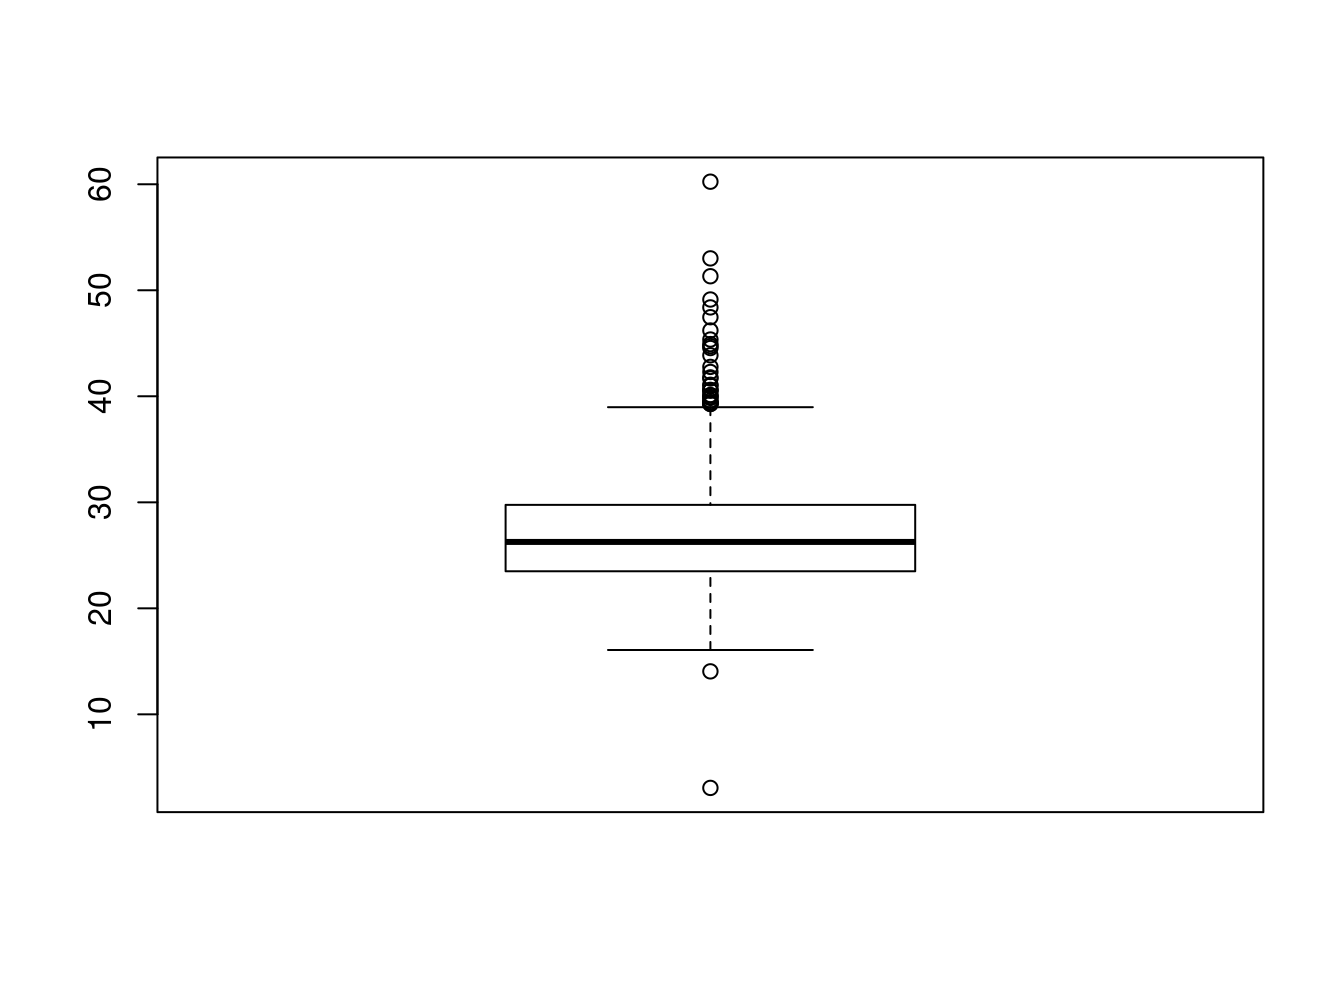
\includegraphics[width=0.8\linewidth]{01-scenario1_files/figure-latex/boxplots-1} \end{center}

\begin{Shaded}
\begin{Highlighting}[]
\OperatorTok{>}\StringTok{ }
\ErrorTok{>}\StringTok{ }\CommentTok{# code using ggplot}
\ErrorTok{>}\StringTok{ }\KeywordTok{library}\NormalTok{(ggplot2)}
\OperatorTok{>}\StringTok{ }\KeywordTok{ggplot}\NormalTok{(dat2, }\KeywordTok{aes}\NormalTok{(}\DataTypeTok{x =} \StringTok{"total"}\NormalTok{, }\DataTypeTok{y =}\NormalTok{ bmi)) }\OperatorTok{+}\StringTok{ }\KeywordTok{geom_boxplot}\NormalTok{()}
\NormalTok{Warning}\OperatorTok{:}\StringTok{ }\NormalTok{Removed }\DecValTok{19}\NormalTok{ rows containing non}\OperatorTok{-}\NormalTok{finite }\KeywordTok{values}\NormalTok{ (stat_boxplot).}
\end{Highlighting}
\end{Shaded}

\begin{center}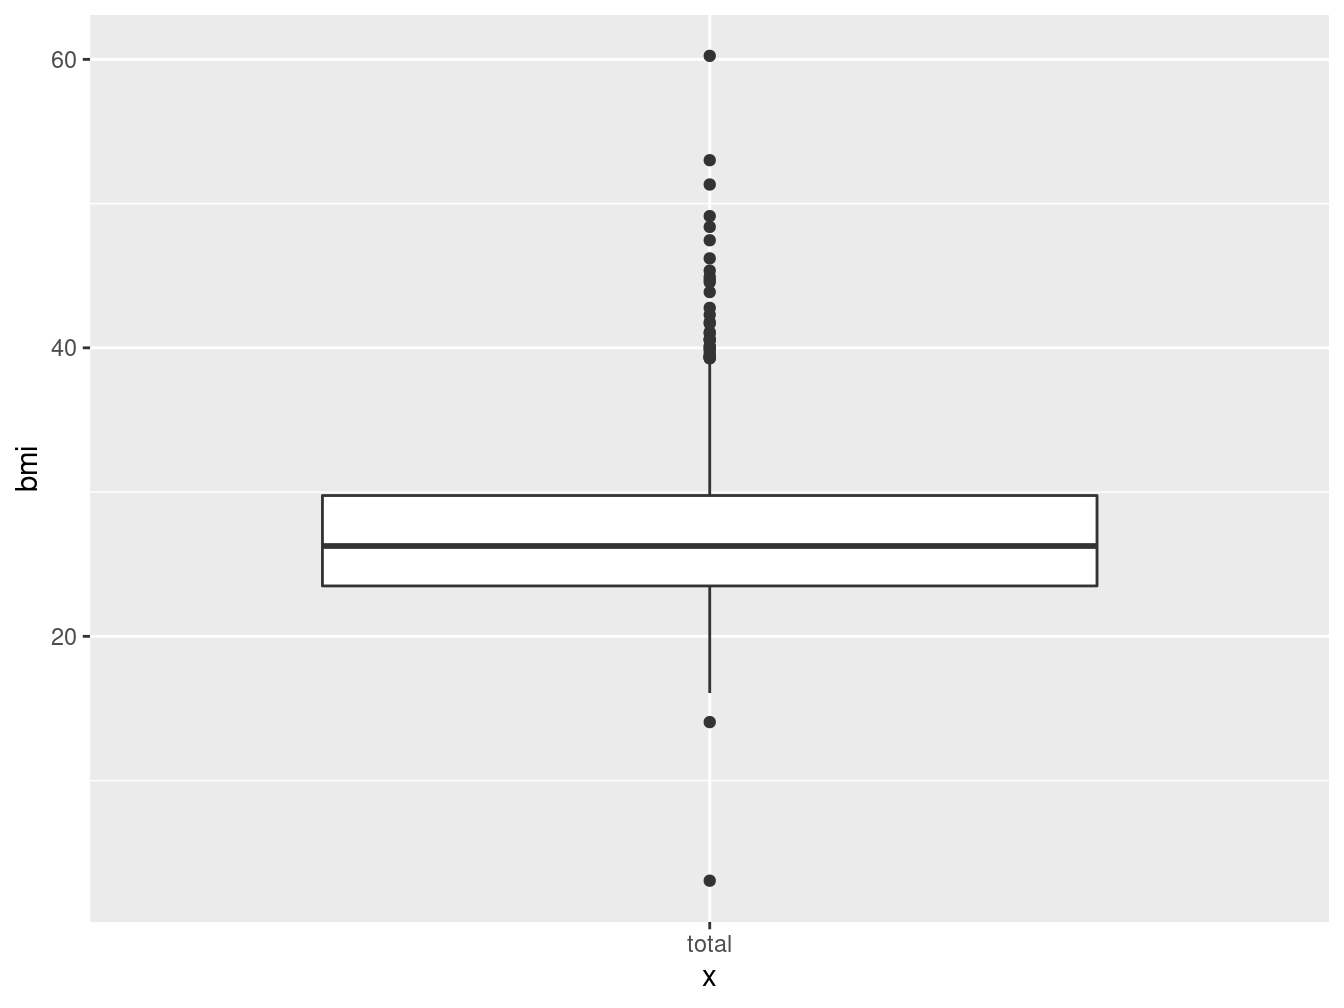
\includegraphics[width=0.8\linewidth]{01-scenario1_files/figure-latex/boxplots-2} \end{center}

\begin{itemize}
\tightlist
\item
  \textbf{Now create the boxplots stratified by the treatment arm}
\end{itemize}

\begin{Shaded}
\begin{Highlighting}[]
\OperatorTok{>}\StringTok{ }\CommentTok{# code using basic R}
\ErrorTok{>}\StringTok{ }\KeywordTok{boxplot}\NormalTok{(bmi }\OperatorTok{~}\StringTok{ }\NormalTok{arm, }\DataTypeTok{data =}\NormalTok{ dat2)}
\end{Highlighting}
\end{Shaded}

\begin{center}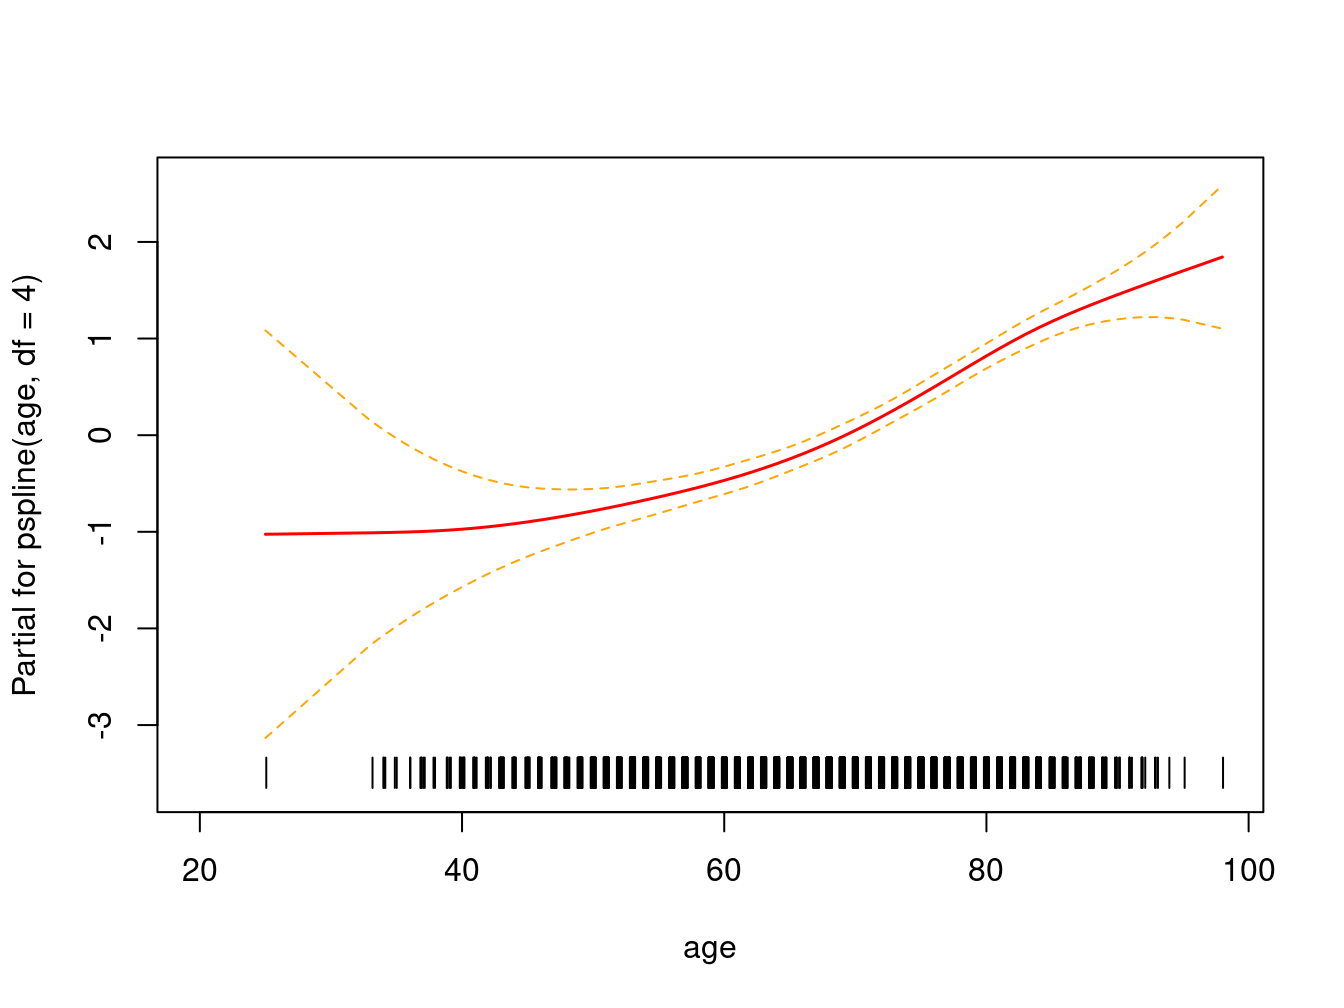
\includegraphics[width=0.8\linewidth]{01-scenario1_files/figure-latex/unnamed-chunk-19-1} \end{center}

\begin{Shaded}
\begin{Highlighting}[]
\OperatorTok{>}\StringTok{ }
\ErrorTok{>}\StringTok{ }\CommentTok{# code using ggplot}
\ErrorTok{>}\StringTok{ }\KeywordTok{ggplot}\NormalTok{(dat2, }\KeywordTok{aes}\NormalTok{(}\DataTypeTok{x =}\NormalTok{ arm, }\DataTypeTok{y =}\NormalTok{ bmi)) }\OperatorTok{+}\StringTok{ }\KeywordTok{geom_boxplot}\NormalTok{()}
\NormalTok{Warning}\OperatorTok{:}\StringTok{ }\NormalTok{Removed }\DecValTok{19}\NormalTok{ rows containing non}\OperatorTok{-}\NormalTok{finite }\KeywordTok{values}\NormalTok{ (stat_boxplot).}
\end{Highlighting}
\end{Shaded}

\begin{center}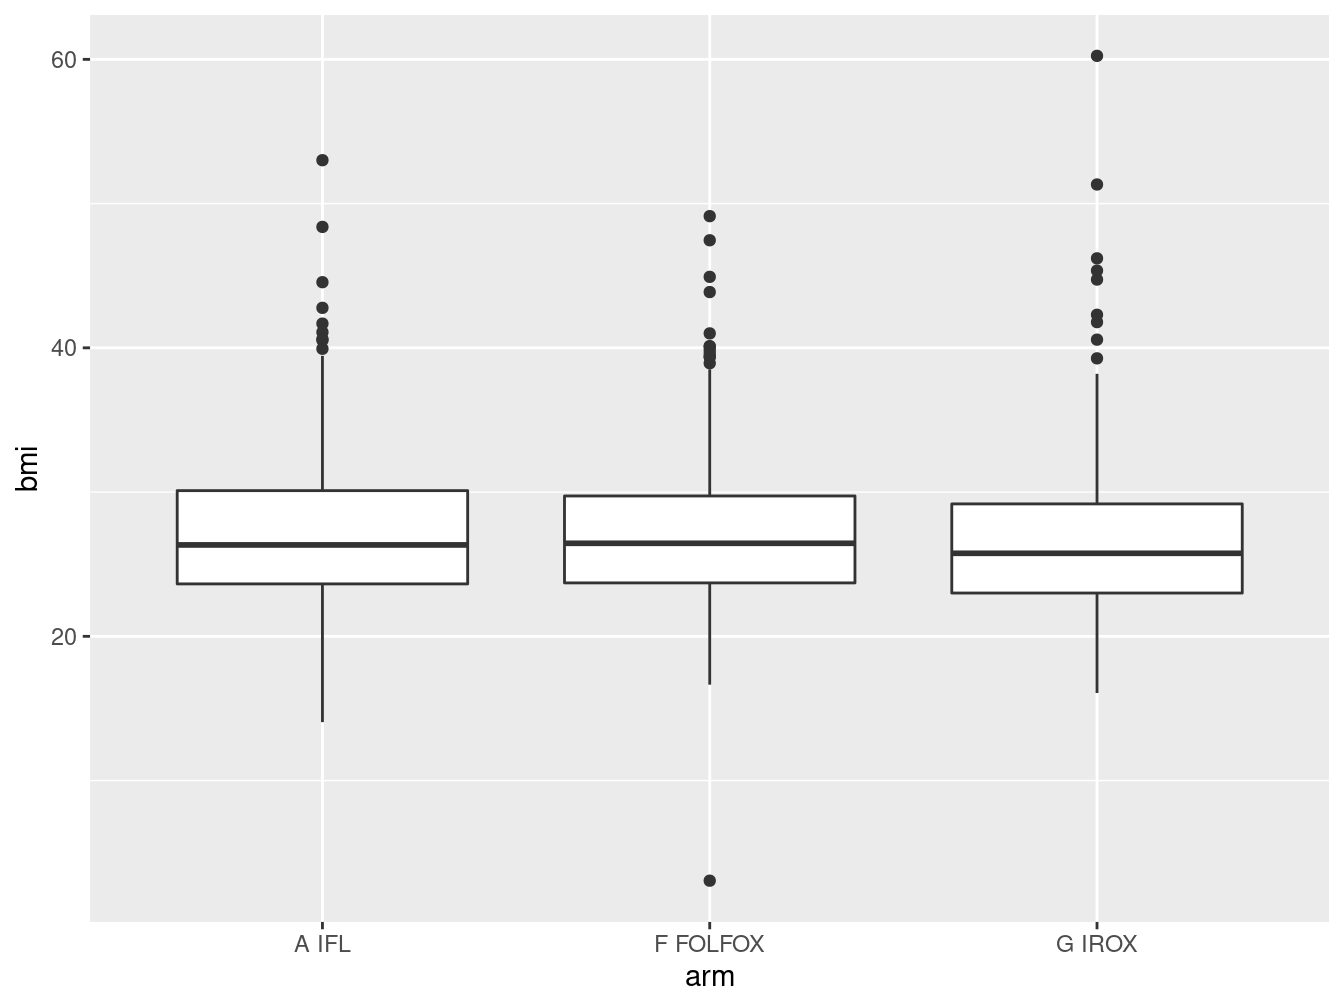
\includegraphics[width=0.8\linewidth]{01-scenario1_files/figure-latex/unnamed-chunk-19-2} \end{center}

\begin{itemize}
\tightlist
\item
  \textbf{Modify the axis labels and add a title to your plot.}
\end{itemize}

\begin{Shaded}
\begin{Highlighting}[]
\OperatorTok{>}\StringTok{ }\CommentTok{# code using basic R}
\ErrorTok{>}\StringTok{ }\KeywordTok{boxplot}\NormalTok{(bmi }\OperatorTok{~}\StringTok{ }\NormalTok{arm, }\DataTypeTok{data =}\NormalTok{ dat2, }\DataTypeTok{xlab =} \StringTok{" "}\NormalTok{, }\DataTypeTok{ylab =} \StringTok{"BMI at baseline"}\NormalTok{, }\DataTypeTok{main =} \StringTok{"BMI distribution stratified by treatment group"}\NormalTok{)}
\end{Highlighting}
\end{Shaded}

\begin{center}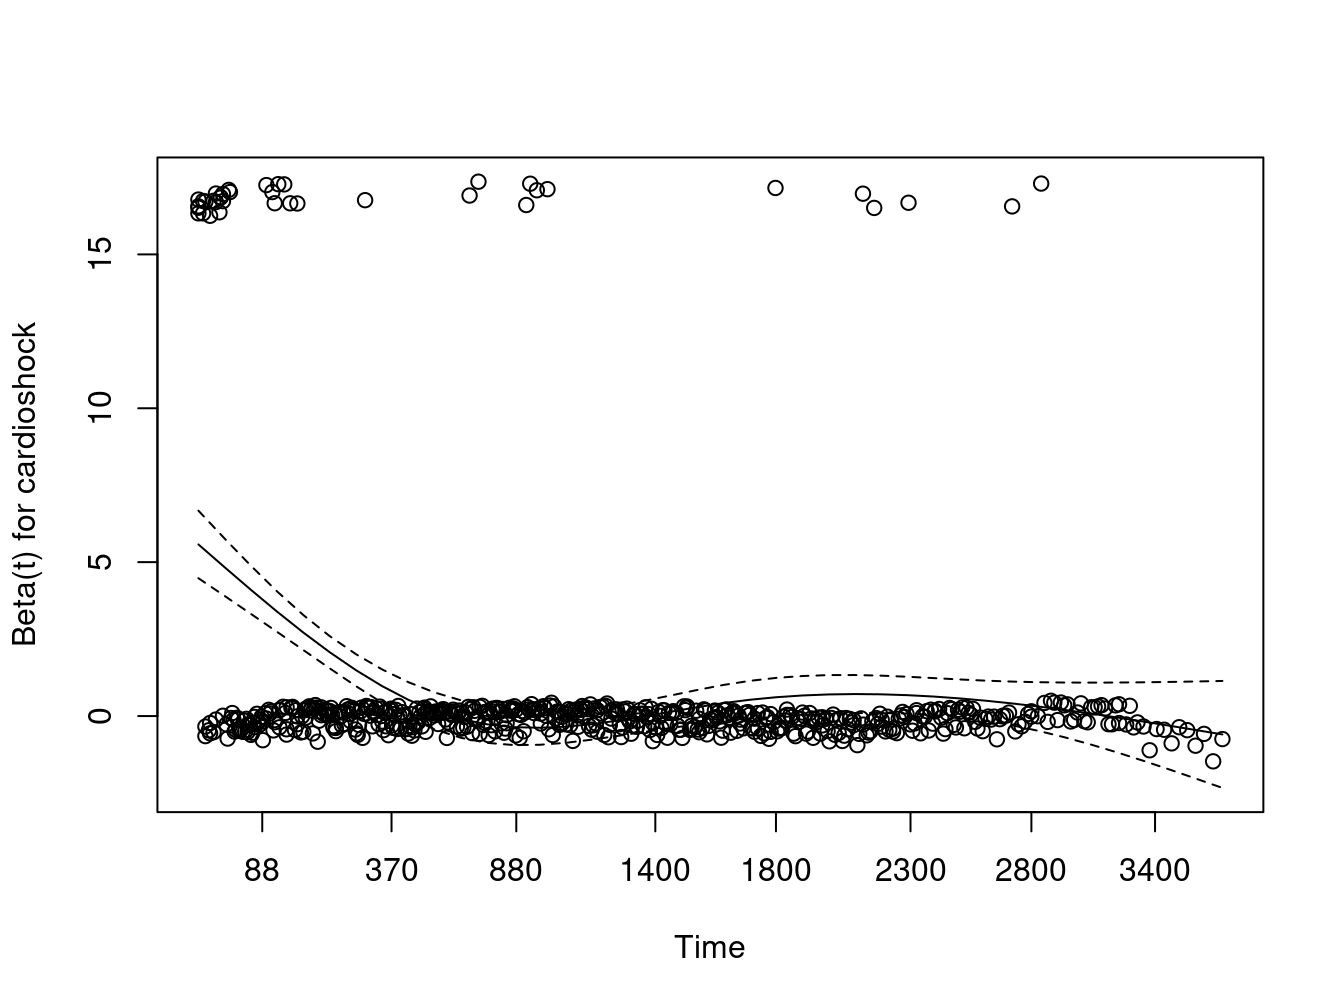
\includegraphics[width=0.8\linewidth]{01-scenario1_files/figure-latex/unnamed-chunk-20-1} \end{center}

\begin{Shaded}
\begin{Highlighting}[]
\OperatorTok{>}\StringTok{ }
\ErrorTok{>}\StringTok{ }\CommentTok{# code using ggplot}
\ErrorTok{>}\StringTok{ }\KeywordTok{ggplot}\NormalTok{(dat2, }\KeywordTok{aes}\NormalTok{(}\DataTypeTok{x =}\NormalTok{ arm, }\DataTypeTok{y =}\NormalTok{ bmi)) }\OperatorTok{+}\StringTok{ }\KeywordTok{geom_boxplot}\NormalTok{() }\OperatorTok{+}\StringTok{ }\KeywordTok{xlab}\NormalTok{(}\StringTok{" "}\NormalTok{) }\OperatorTok{+}\StringTok{ }\KeywordTok{ylab}\NormalTok{(}\StringTok{"BMI at baseline"}\NormalTok{) }\OperatorTok{+}\StringTok{ }
\OperatorTok{+}\StringTok{     }\KeywordTok{ggtitle}\NormalTok{(}\StringTok{"BMI distribution stratified by treatment group"}\NormalTok{)}
\NormalTok{Warning}\OperatorTok{:}\StringTok{ }\NormalTok{Removed }\DecValTok{19}\NormalTok{ rows containing non}\OperatorTok{-}\NormalTok{finite }\KeywordTok{values}\NormalTok{ (stat_boxplot).}
\end{Highlighting}
\end{Shaded}

\begin{center}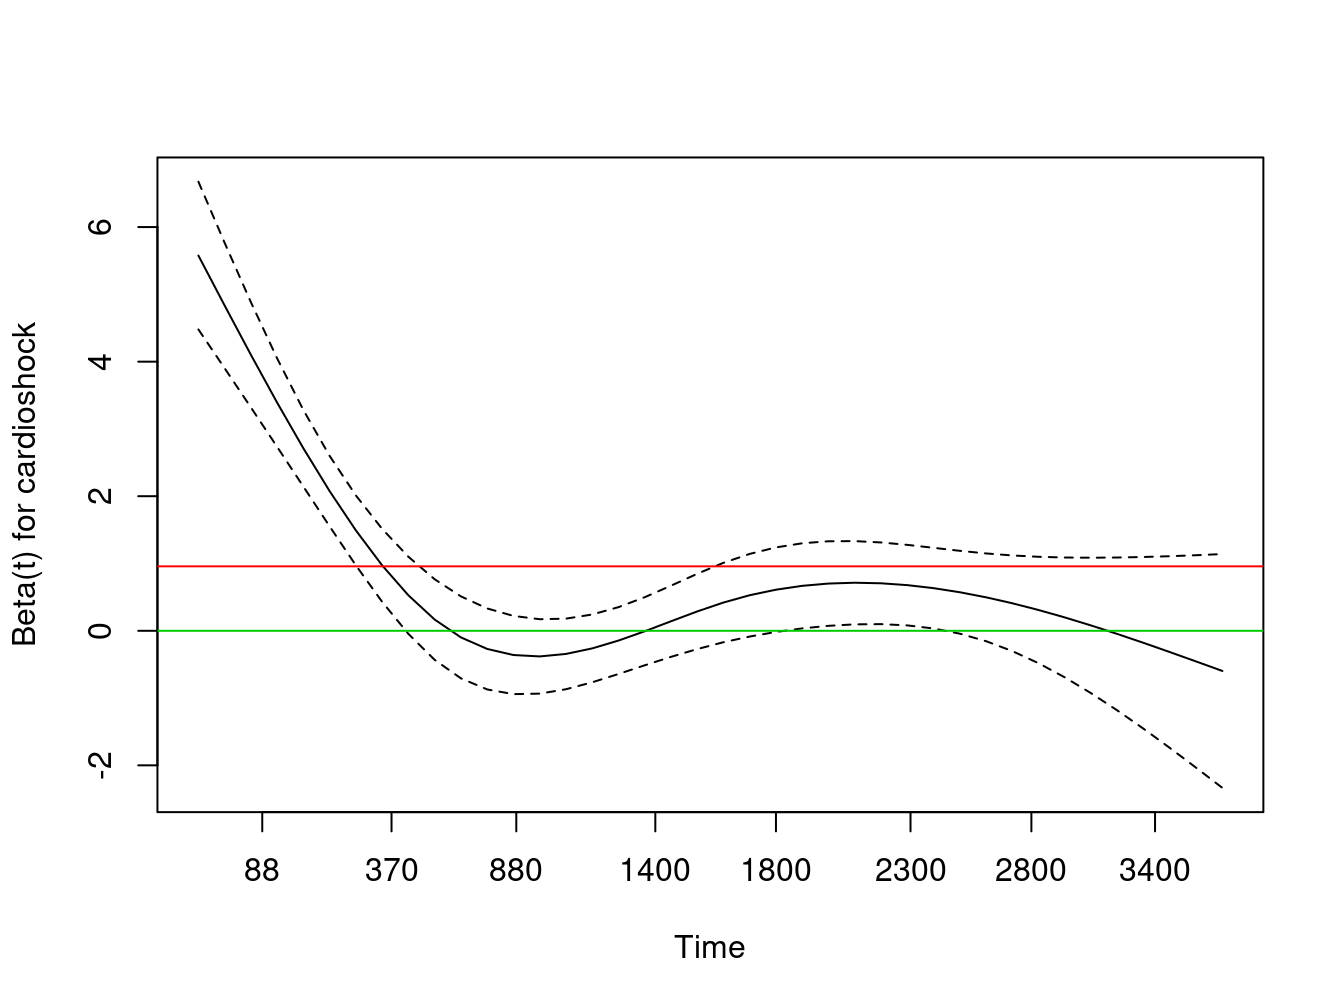
\includegraphics[width=0.8\linewidth]{01-scenario1_files/figure-latex/unnamed-chunk-20-2} \end{center}

\hypertarget{scatterplots}{%
\subsubsection{Scatterplots}\label{scatterplots}}

\begin{itemize}
\tightlist
\item
  \textbf{Now make two scatterplots of age versus bmi with different colors indicating treatment}
\end{itemize}

The call to \texttt{as.numeric(as.factor(arm))} turns the levels of \texttt{arm} to a factor which is essentially a numeric variables with formats. The call to \texttt{as.numeric} then changes the factor to a number, and the numbers correspond to different colors (1=black, 2=red, 3=green, 4=blue, 5=lightblue, 6=pink, 7=yellow, 8=gray).

\begin{Shaded}
\begin{Highlighting}[]
\OperatorTok{>}\StringTok{ }\CommentTok{# code using basic R}
\ErrorTok{>}\StringTok{ }\KeywordTok{plot}\NormalTok{(bmi }\OperatorTok{~}\StringTok{ }\NormalTok{age, }\DataTypeTok{data =}\NormalTok{ dat2, }\DataTypeTok{col =} \KeywordTok{as.numeric}\NormalTok{(}\KeywordTok{as.factor}\NormalTok{(arm)))}
\end{Highlighting}
\end{Shaded}

\begin{center}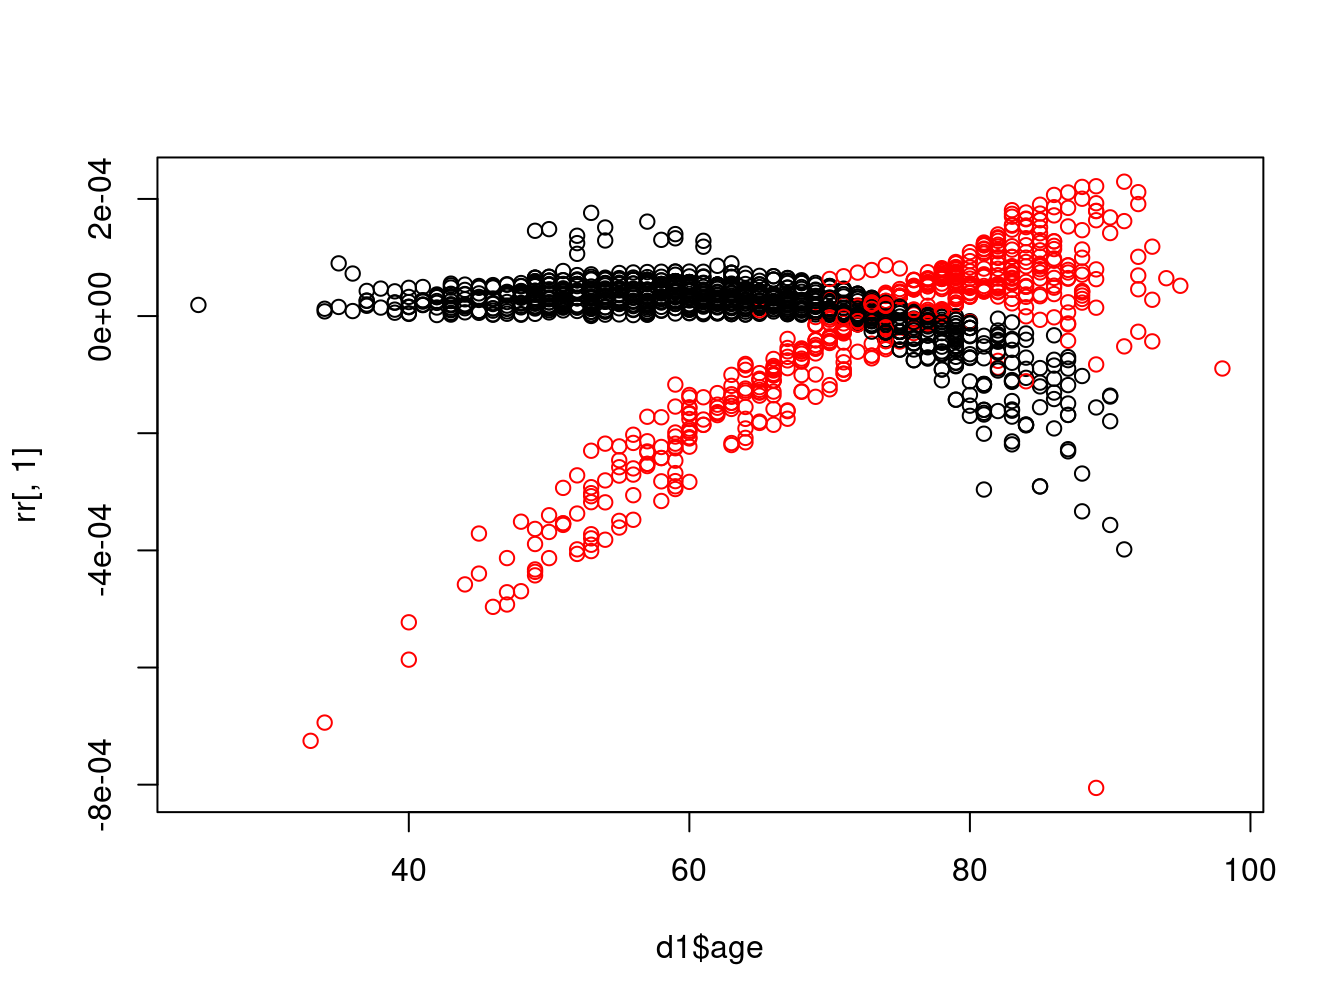
\includegraphics[width=0.8\linewidth]{01-scenario1_files/figure-latex/unnamed-chunk-21-1} \end{center}

\begin{Shaded}
\begin{Highlighting}[]
\OperatorTok{>}\StringTok{ }
\ErrorTok{>}\StringTok{ }\CommentTok{# code using ggplot}
\ErrorTok{>}\StringTok{ }\KeywordTok{ggplot}\NormalTok{(dat2, }\KeywordTok{aes}\NormalTok{(age, bmi, }\DataTypeTok{color =}\NormalTok{ arm)) }\OperatorTok{+}\StringTok{ }\KeywordTok{geom_point}\NormalTok{()}
\NormalTok{Warning}\OperatorTok{:}\StringTok{ }\NormalTok{Removed }\DecValTok{19}\NormalTok{ rows containing missing }\KeywordTok{values}\NormalTok{ (geom_point).}
\end{Highlighting}
\end{Shaded}

\begin{center}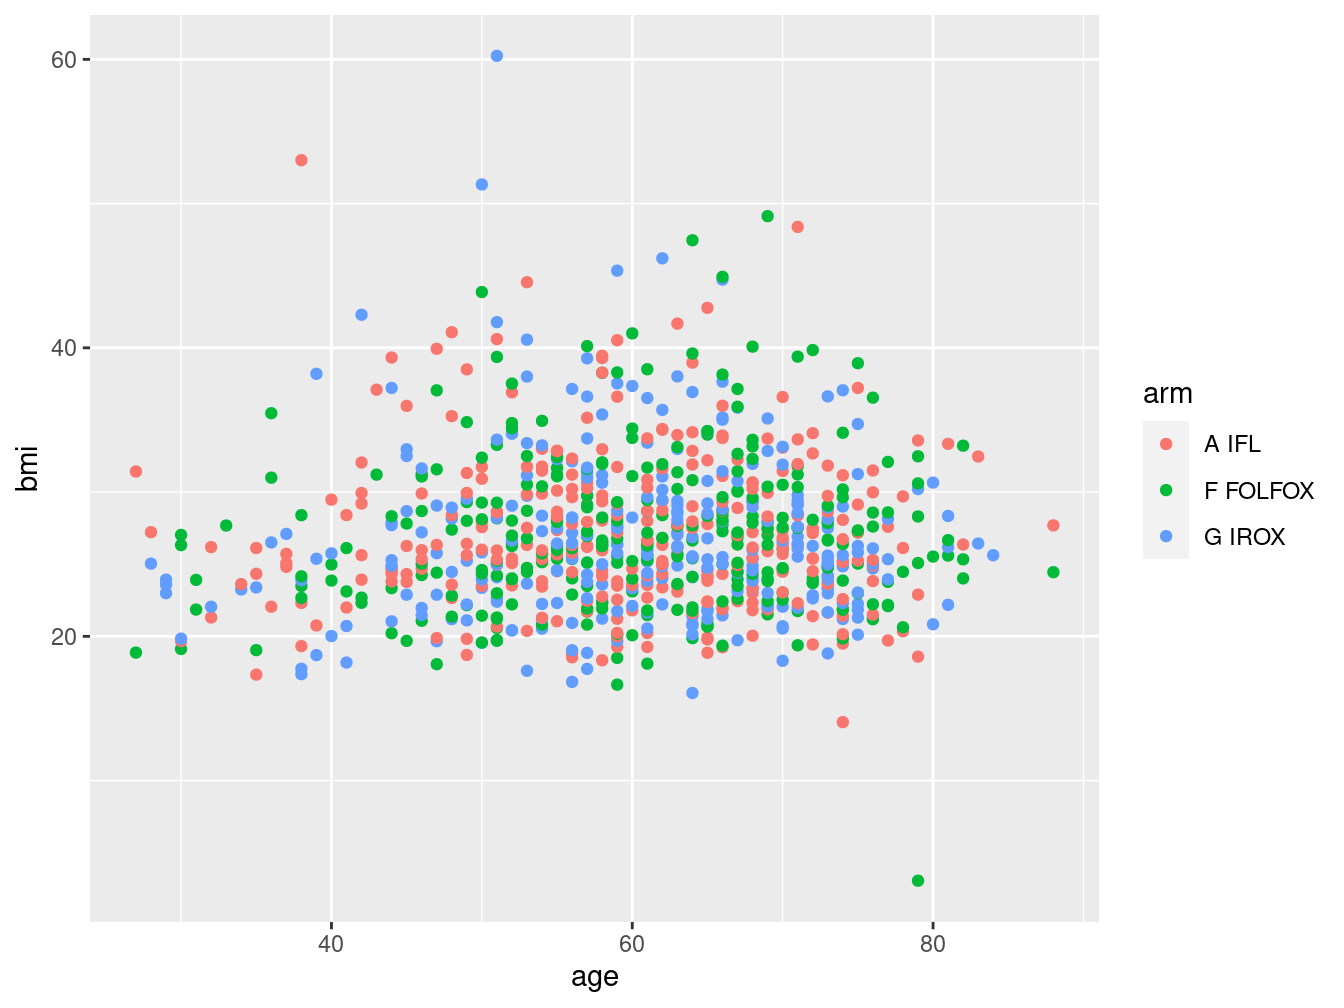
\includegraphics[width=0.8\linewidth]{01-scenario1_files/figure-latex/unnamed-chunk-21-2} \end{center}

\begin{itemize}
\tightlist
\item
  \textbf{Create these same scatterplots, side-by-side, separately for males and females}
\end{itemize}

\begin{Shaded}
\begin{Highlighting}[]
\OperatorTok{>}\StringTok{ }\CommentTok{# code using basic R}
\ErrorTok{>}\StringTok{ }\KeywordTok{par}\NormalTok{(}\DataTypeTok{mfrow =} \KeywordTok{c}\NormalTok{(}\DecValTok{1}\NormalTok{, }\DecValTok{2}\NormalTok{))}
\OperatorTok{>}\StringTok{ }\KeywordTok{plot}\NormalTok{(bmi }\OperatorTok{~}\StringTok{ }\NormalTok{age, }\DataTypeTok{data =}\NormalTok{ dat2[dat2}\OperatorTok{$}\NormalTok{sex }\OperatorTok{==}\StringTok{ "Female"}\NormalTok{, ], }\DataTypeTok{col =} \KeywordTok{as.numeric}\NormalTok{(}\KeywordTok{as.factor}\NormalTok{(arm)), }
\OperatorTok{+}\StringTok{     }\DataTypeTok{main =} \StringTok{"Females"}\NormalTok{)}
\OperatorTok{>}\StringTok{ }\KeywordTok{plot}\NormalTok{(bmi }\OperatorTok{~}\StringTok{ }\NormalTok{age, }\DataTypeTok{data =}\NormalTok{ dat2[dat2}\OperatorTok{$}\NormalTok{sex }\OperatorTok{==}\StringTok{ "Male"}\NormalTok{, ], }\DataTypeTok{col =} \KeywordTok{as.numeric}\NormalTok{(}\KeywordTok{as.factor}\NormalTok{(arm)), }
\OperatorTok{+}\StringTok{     }\DataTypeTok{main =} \StringTok{"Males"}\NormalTok{)}
\end{Highlighting}
\end{Shaded}

\begin{center}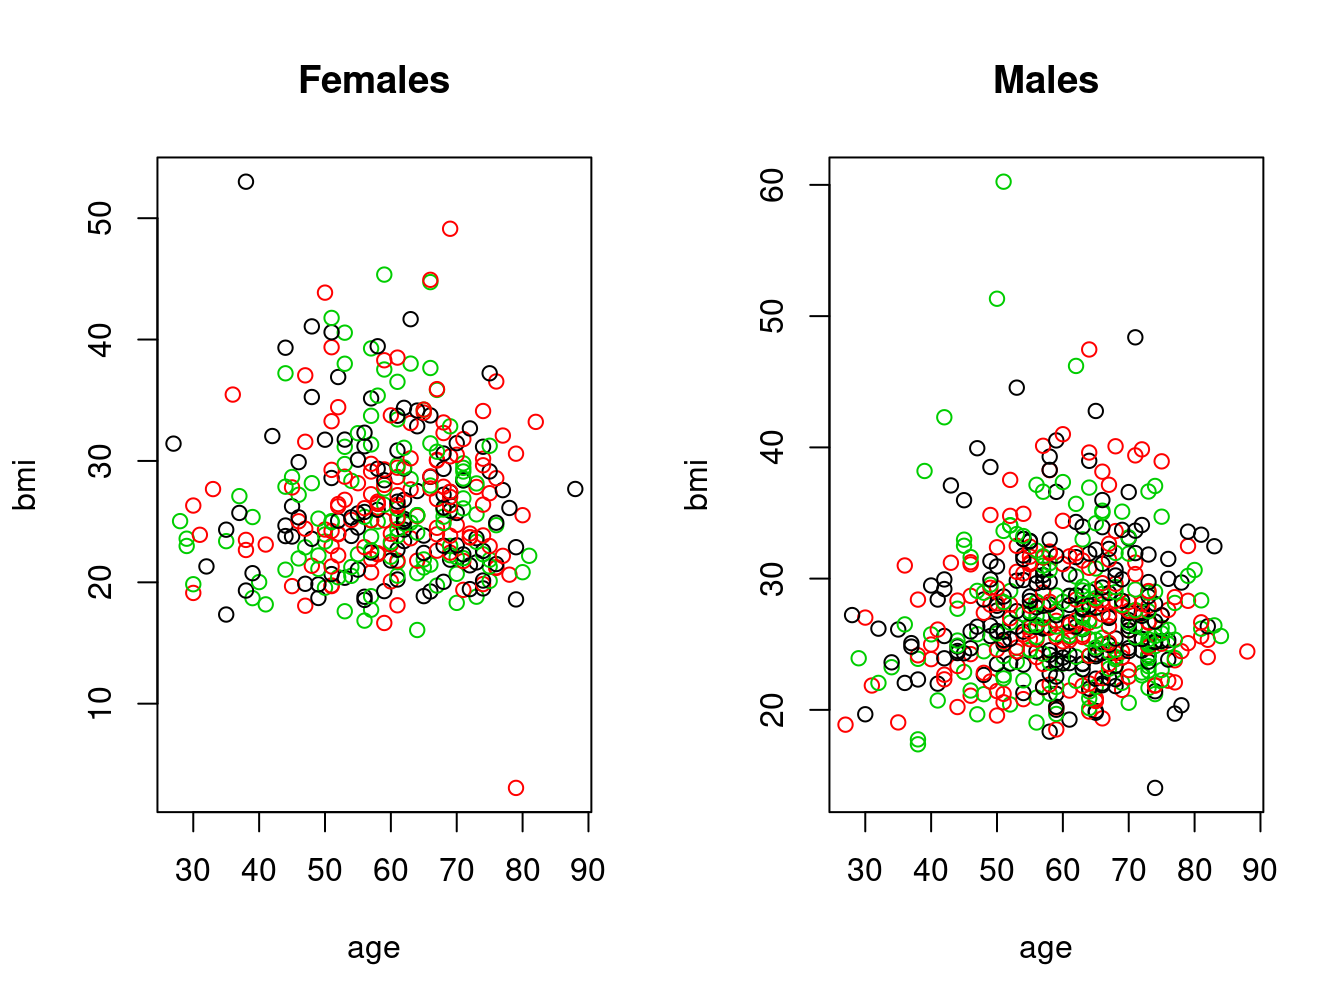
\includegraphics[width=0.8\linewidth]{01-scenario1_files/figure-latex/unnamed-chunk-22-1} \end{center}

\begin{Shaded}
\begin{Highlighting}[]
\OperatorTok{>}\StringTok{ }\KeywordTok{par}\NormalTok{(}\DataTypeTok{mfrow =} \KeywordTok{c}\NormalTok{(}\DecValTok{1}\NormalTok{, }\DecValTok{1}\NormalTok{))}
\OperatorTok{>}\StringTok{ }
\ErrorTok{>}\StringTok{ }\CommentTok{# code using ggplot}
\ErrorTok{>}\StringTok{ }\KeywordTok{ggplot}\NormalTok{(dat2, }\KeywordTok{aes}\NormalTok{(age, bmi, }\DataTypeTok{color =}\NormalTok{ arm)) }\OperatorTok{+}\StringTok{ }\KeywordTok{geom_point}\NormalTok{() }\OperatorTok{+}\StringTok{ }\KeywordTok{facet_grid}\NormalTok{(}\OperatorTok{~}\NormalTok{sex)}
\NormalTok{Warning}\OperatorTok{:}\StringTok{ }\NormalTok{Removed }\DecValTok{19}\NormalTok{ rows containing missing }\KeywordTok{values}\NormalTok{ (geom_point).}
\end{Highlighting}
\end{Shaded}

\begin{center}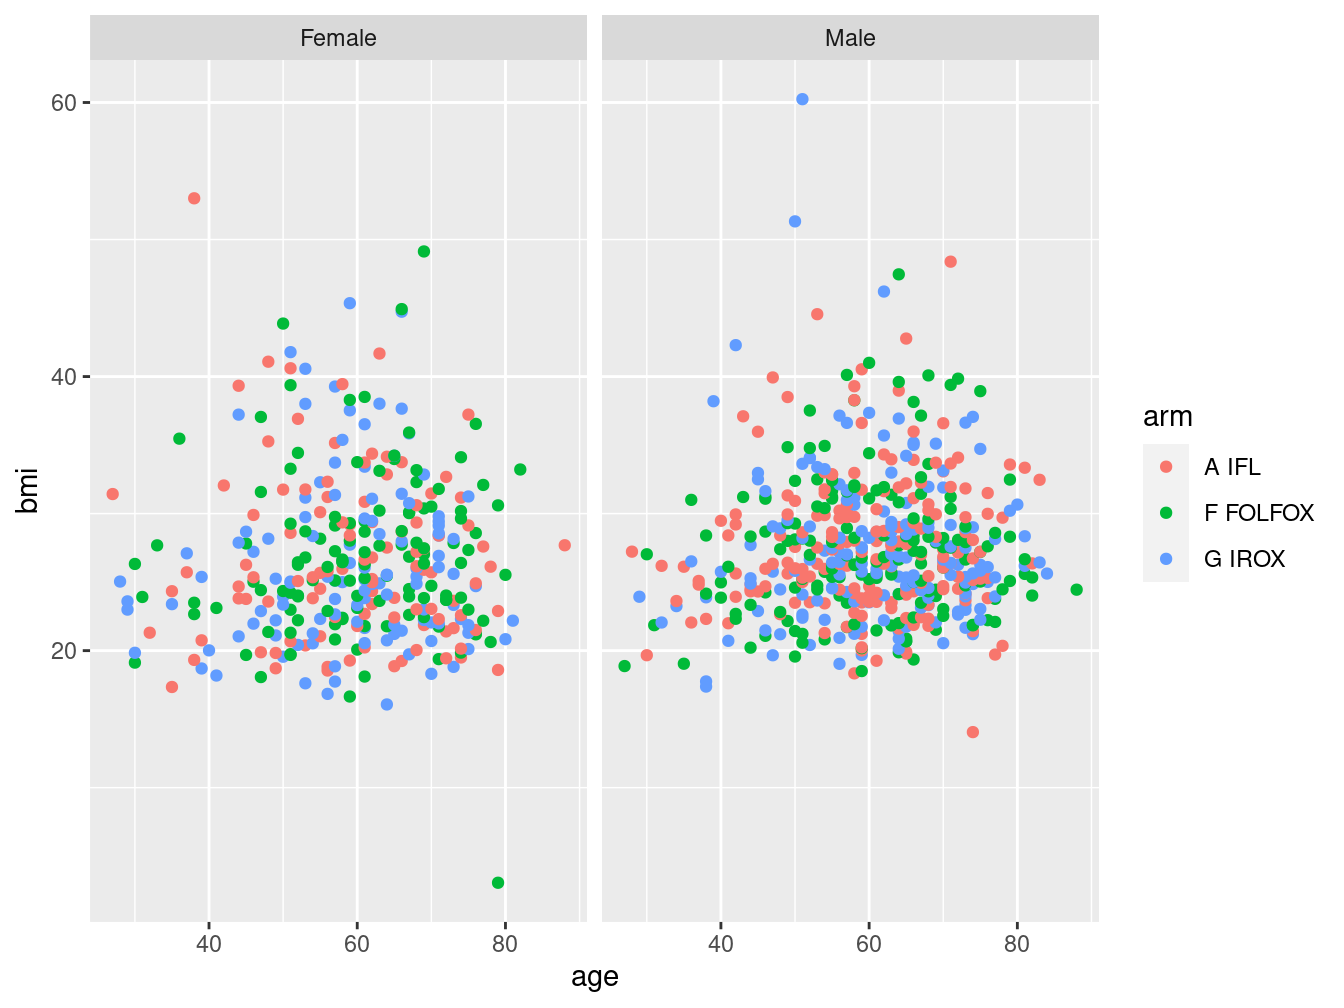
\includegraphics[width=0.8\linewidth]{01-scenario1_files/figure-latex/unnamed-chunk-22-2} \end{center}

\begin{itemize}
\tightlist
\item
  \textbf{Fancier: How would you add a regression line to these plots? How about smoothers?}
\end{itemize}

The code using base R graphics can be found further down at the \protect\hyperlink{alt-plot}{end of this document}.

\begin{Shaded}
\begin{Highlighting}[]
\OperatorTok{>}\StringTok{ }\CommentTok{# code using ggplot -- Regression lines}
\ErrorTok{>}\StringTok{ }\KeywordTok{ggplot}\NormalTok{(dat2, }\KeywordTok{aes}\NormalTok{(age, bmi, }\DataTypeTok{color =}\NormalTok{ arm)) }\OperatorTok{+}\StringTok{ }\KeywordTok{geom_point}\NormalTok{() }\OperatorTok{+}\StringTok{ }\KeywordTok{facet_grid}\NormalTok{(}\OperatorTok{~}\NormalTok{sex) }\OperatorTok{+}\StringTok{ }\KeywordTok{geom_smooth}\NormalTok{(}\DataTypeTok{method =} \StringTok{"lm"}\NormalTok{)}
\StringTok{`}\DataTypeTok{geom_smooth()}\StringTok{`}\NormalTok{ using formula }\StringTok{'y ~ x'}
\NormalTok{Warning}\OperatorTok{:}\StringTok{ }\NormalTok{Removed }\DecValTok{19}\NormalTok{ rows containing non}\OperatorTok{-}\NormalTok{finite }\KeywordTok{values}\NormalTok{ (stat_smooth).}
\NormalTok{Warning}\OperatorTok{:}\StringTok{ }\NormalTok{Removed }\DecValTok{19}\NormalTok{ rows containing missing }\KeywordTok{values}\NormalTok{ (geom_point).}
\end{Highlighting}
\end{Shaded}

\begin{center}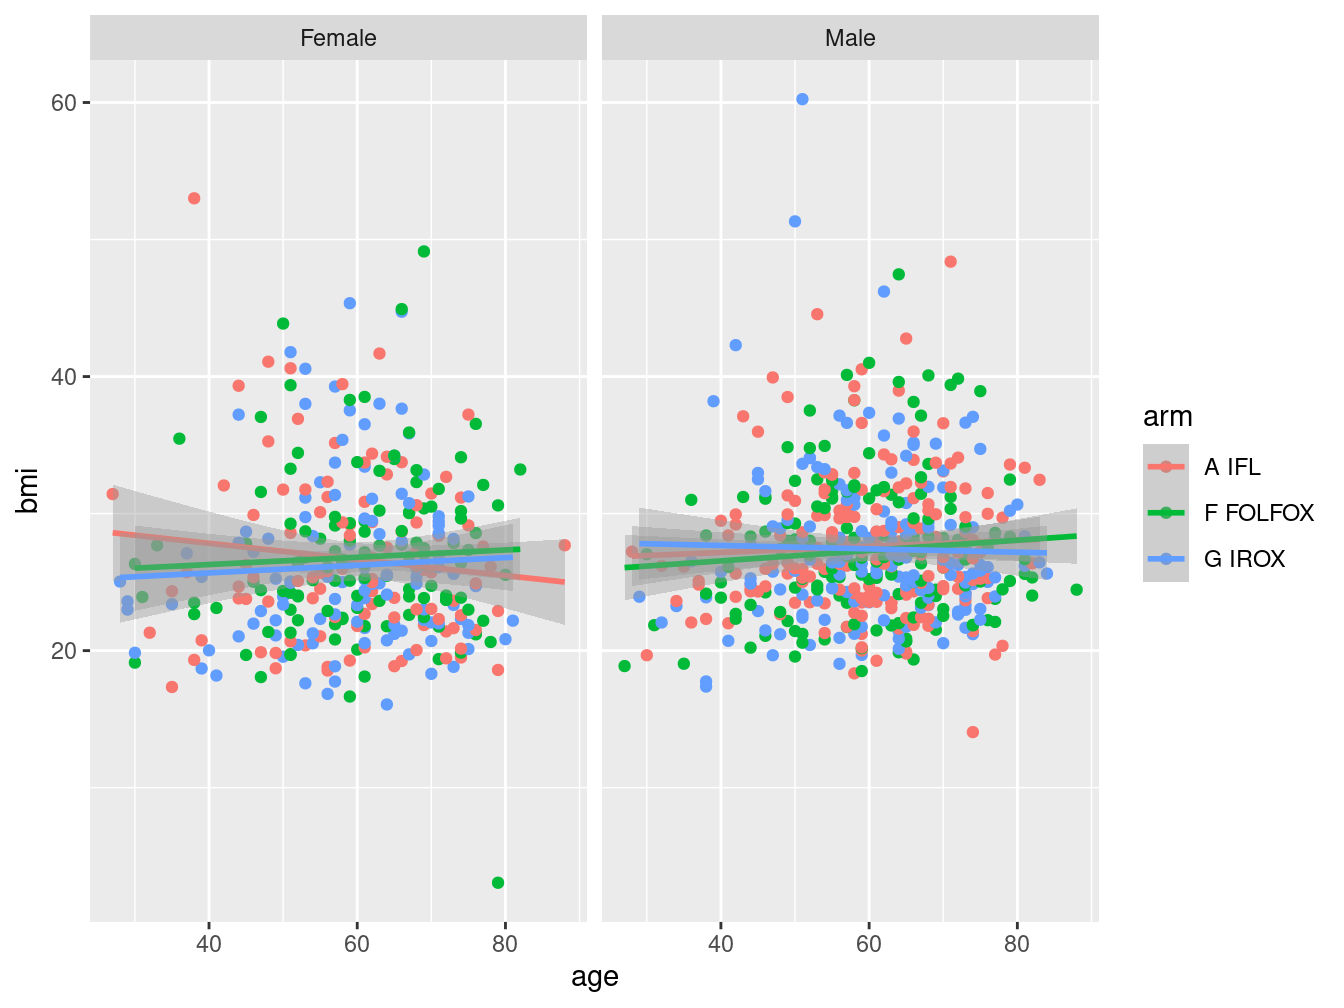
\includegraphics[width=0.8\linewidth]{01-scenario1_files/figure-latex/unnamed-chunk-23-1} \end{center}

\begin{Shaded}
\begin{Highlighting}[]
\OperatorTok{>}\StringTok{ }
\ErrorTok{>}\StringTok{ }\CommentTok{# -- Smoothers}
\ErrorTok{>}\StringTok{ }\KeywordTok{ggplot}\NormalTok{(dat2, }\KeywordTok{aes}\NormalTok{(age, bmi, }\DataTypeTok{color =}\NormalTok{ arm)) }\OperatorTok{+}\StringTok{ }\KeywordTok{geom_point}\NormalTok{() }\OperatorTok{+}\StringTok{ }\KeywordTok{facet_grid}\NormalTok{(}\OperatorTok{~}\NormalTok{sex) }\OperatorTok{+}\StringTok{ }\KeywordTok{geom_smooth}\NormalTok{()}
\StringTok{`}\DataTypeTok{geom_smooth()}\StringTok{`}\NormalTok{ using method =}\StringTok{ 'loess'}\NormalTok{ and formula }\StringTok{'y ~ x'}
\NormalTok{Warning}\OperatorTok{:}\StringTok{ }\NormalTok{Removed }\DecValTok{19}\NormalTok{ rows containing non}\OperatorTok{-}\NormalTok{finite }\KeywordTok{values}\NormalTok{ (stat_smooth).}

\NormalTok{Warning}\OperatorTok{:}\StringTok{ }\NormalTok{Removed }\DecValTok{19}\NormalTok{ rows containing missing }\KeywordTok{values}\NormalTok{ (geom_point).}
\end{Highlighting}
\end{Shaded}

\begin{center}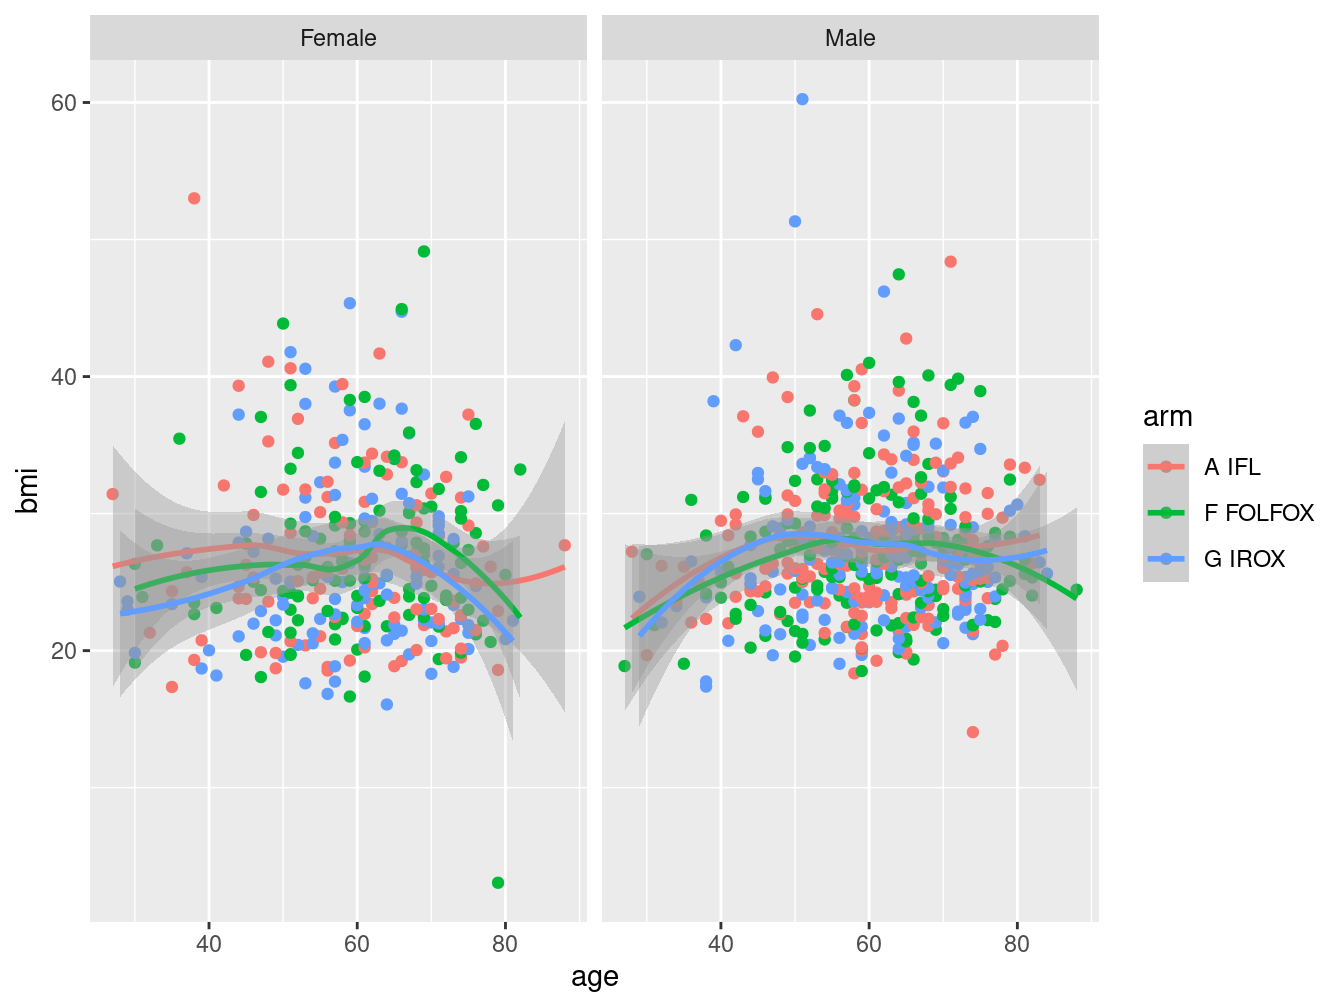
\includegraphics[width=0.8\linewidth]{01-scenario1_files/figure-latex/unnamed-chunk-23-2} \end{center}

\begin{Shaded}
\begin{Highlighting}[]
\OperatorTok{>}\StringTok{ }
\ErrorTok{>}\StringTok{ }\CommentTok{# -- Smoothers removing the confidence bands}
\ErrorTok{>}\StringTok{ }\KeywordTok{ggplot}\NormalTok{(dat2, }\KeywordTok{aes}\NormalTok{(age, bmi, }\DataTypeTok{color =}\NormalTok{ arm)) }\OperatorTok{+}\StringTok{ }\KeywordTok{geom_point}\NormalTok{() }\OperatorTok{+}\StringTok{ }\KeywordTok{facet_grid}\NormalTok{(}\OperatorTok{~}\NormalTok{sex) }\OperatorTok{+}\StringTok{ }\KeywordTok{geom_smooth}\NormalTok{(}\DataTypeTok{se =} \OtherTok{FALSE}\NormalTok{)}
\StringTok{`}\DataTypeTok{geom_smooth()}\StringTok{`}\NormalTok{ using method =}\StringTok{ 'loess'}\NormalTok{ and formula }\StringTok{'y ~ x'}
\NormalTok{Warning}\OperatorTok{:}\StringTok{ }\NormalTok{Removed }\DecValTok{19}\NormalTok{ rows containing non}\OperatorTok{-}\NormalTok{finite }\KeywordTok{values}\NormalTok{ (stat_smooth).}

\NormalTok{Warning}\OperatorTok{:}\StringTok{ }\NormalTok{Removed }\DecValTok{19}\NormalTok{ rows containing missing }\KeywordTok{values}\NormalTok{ (geom_point).}
\end{Highlighting}
\end{Shaded}

\begin{center}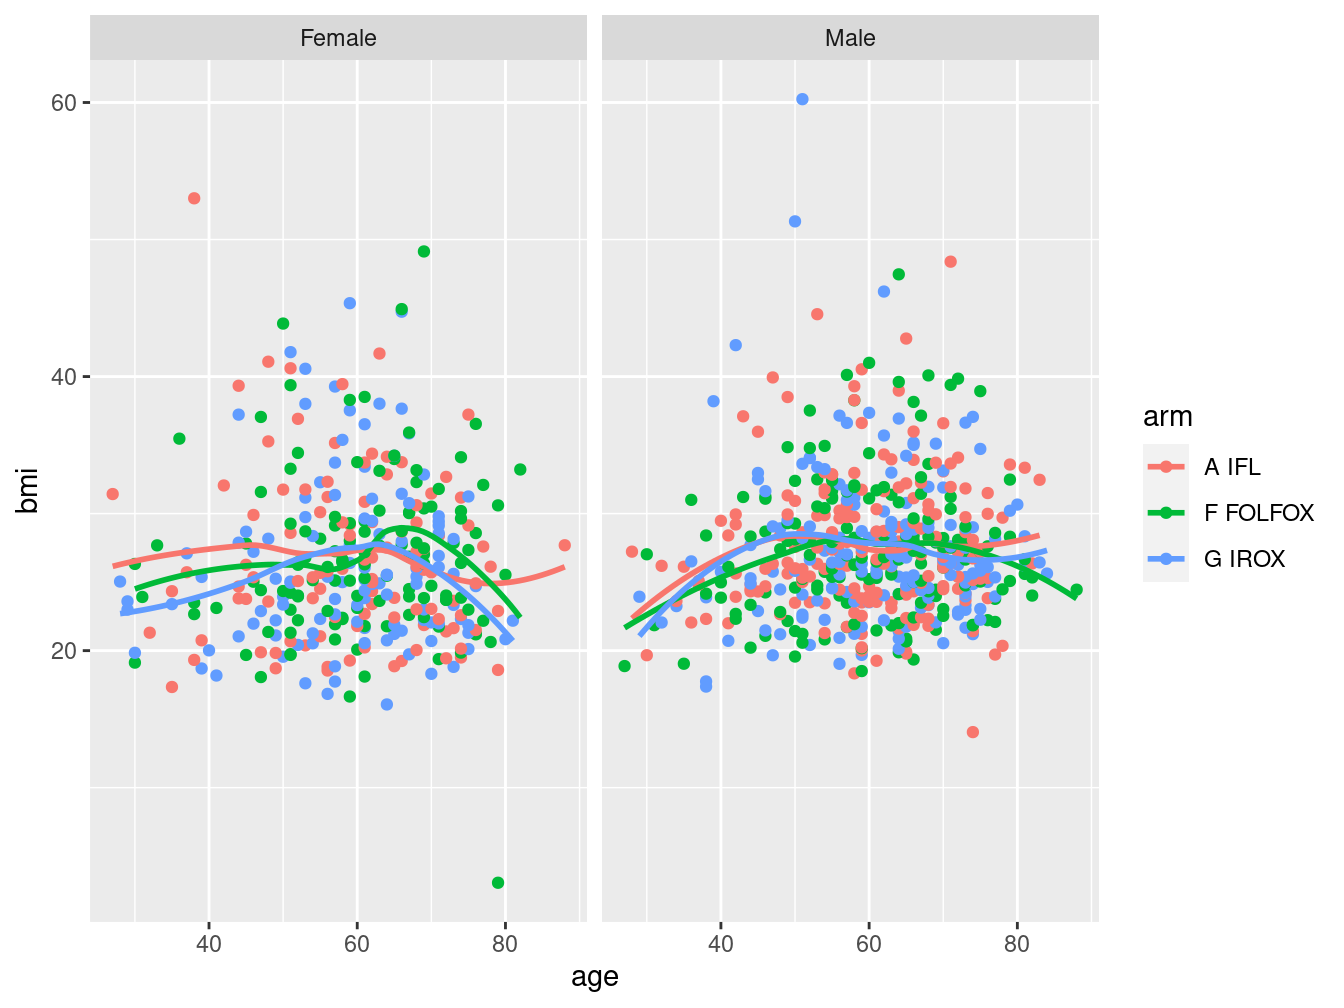
\includegraphics[width=0.8\linewidth]{01-scenario1_files/figure-latex/unnamed-chunk-23-3} \end{center}

There are many formating options for \texttt{ggplot} including \texttt{theme\_bw} and the package {[}ggthemes{[}(\url{https://rdrr.io/cran/ggthemes/}){]} which includes extra themes, geoms, and scales for ggplot2. Below, see how the plot has changed by just indicating the plotting theme. Another addition is the \texttt{alpha} term which lightens the points (default=1).

\begin{Shaded}
\begin{Highlighting}[]
\OperatorTok{>}\StringTok{ }\KeywordTok{ggplot}\NormalTok{(dat2, }\KeywordTok{aes}\NormalTok{(age, bmi, }\DataTypeTok{color =}\NormalTok{ arm)) }\OperatorTok{+}\StringTok{ }\KeywordTok{geom_point}\NormalTok{(}\DataTypeTok{alpha =} \FloatTok{0.2}\NormalTok{) }\OperatorTok{+}\StringTok{ }\KeywordTok{facet_grid}\NormalTok{(}\OperatorTok{~}\NormalTok{sex) }\OperatorTok{+}\StringTok{ }
\OperatorTok{+}\StringTok{     }\KeywordTok{geom_smooth}\NormalTok{(}\DataTypeTok{se =} \OtherTok{FALSE}\NormalTok{) }\OperatorTok{+}\StringTok{ }\KeywordTok{theme_bw}\NormalTok{()}
\StringTok{`}\DataTypeTok{geom_smooth()}\StringTok{`}\NormalTok{ using method =}\StringTok{ 'loess'}\NormalTok{ and formula }\StringTok{'y ~ x'}
\NormalTok{Warning}\OperatorTok{:}\StringTok{ }\NormalTok{Removed }\DecValTok{19}\NormalTok{ rows containing non}\OperatorTok{-}\NormalTok{finite }\KeywordTok{values}\NormalTok{ (stat_smooth).}
\NormalTok{Warning}\OperatorTok{:}\StringTok{ }\NormalTok{Removed }\DecValTok{19}\NormalTok{ rows containing missing }\KeywordTok{values}\NormalTok{ (geom_point).}
\end{Highlighting}
\end{Shaded}

\begin{center}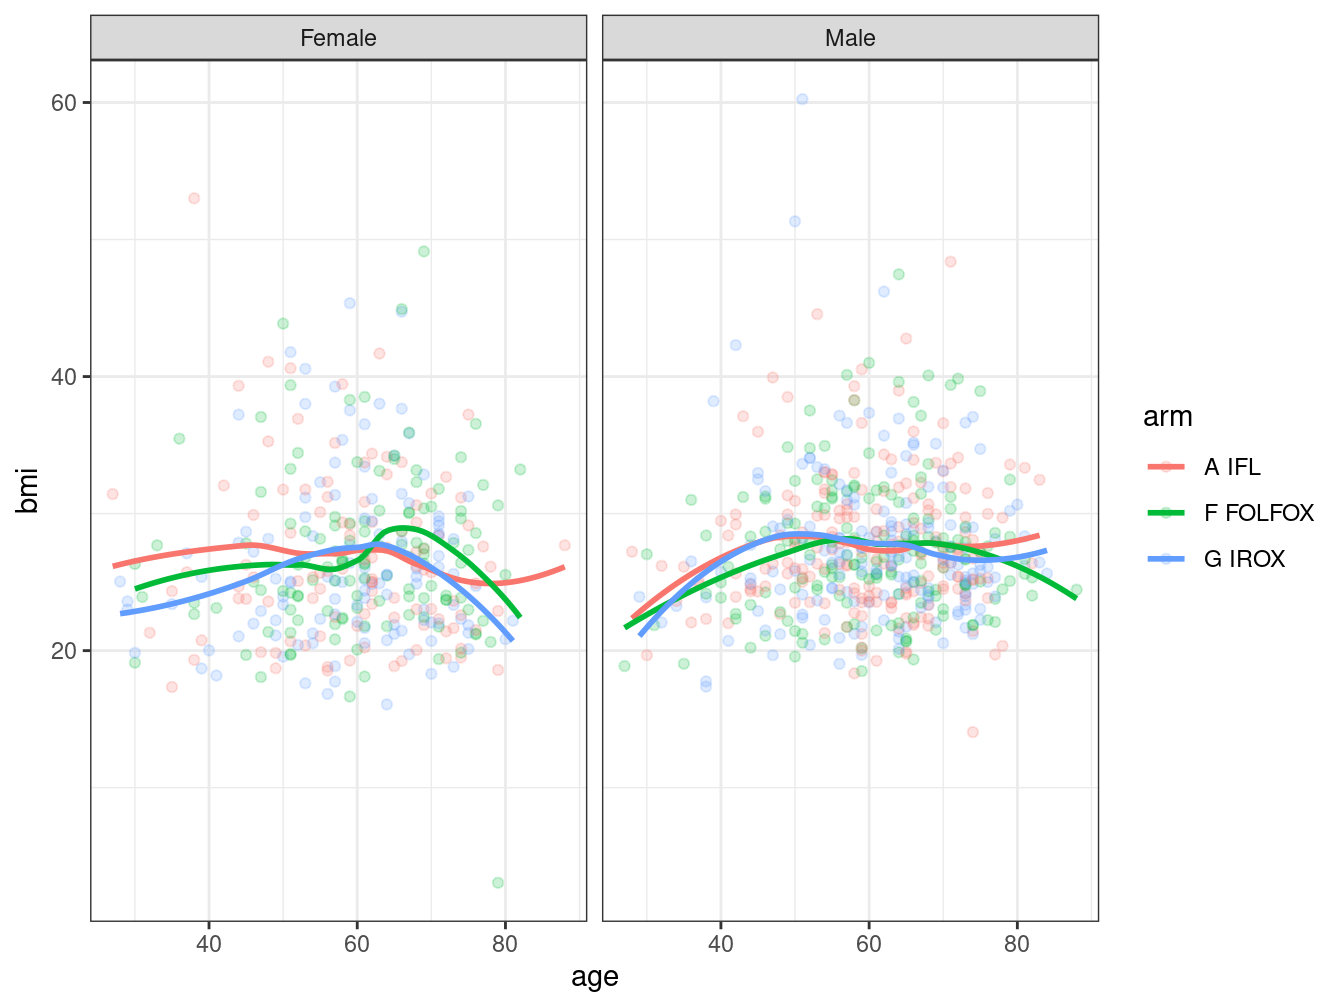
\includegraphics[width=0.8\linewidth]{01-scenario1_files/figure-latex/unnamed-chunk-24-1} \end{center}

\hypertarget{basic-modeling}{%
\subsection{Basic Modeling}\label{basic-modeling}}

\begin{itemize}
\tightlist
\item
  \textbf{Run a simple linear regression model predicting bmi with a covariate that is coded as 1/2. Now re-do it with the covariate coded as a factor. Did the answer change?}
\end{itemize}

First create a numeric version of sex with the values 1 and 2 (for illustration purposes only). This can be done by changing the variable \texttt{sex} from character to a factor, then changing the factor to numeric.

\begin{Shaded}
\begin{Highlighting}[]
\OperatorTok{>}\StringTok{ }\CommentTok{# Create a version of sex that is coded 1/2}
\ErrorTok{>}\StringTok{ }\NormalTok{dat2}\OperatorTok{$}\NormalTok{sex.f <-}\StringTok{ }\KeywordTok{factor}\NormalTok{(dat2}\OperatorTok{$}\NormalTok{sex)}
\OperatorTok{>}\StringTok{ }\NormalTok{dat2}\OperatorTok{$}\NormalTok{sex12 <-}\StringTok{ }\KeywordTok{as.numeric}\NormalTok{(dat2}\OperatorTok{$}\NormalTok{sex.f)}
\OperatorTok{>}\StringTok{ }
\ErrorTok{>}\StringTok{ }\KeywordTok{table}\NormalTok{(dat2}\OperatorTok{$}\NormalTok{sex12, dat2}\OperatorTok{$}\NormalTok{sex.f)}
   
\NormalTok{    Female Male}
  \DecValTok{1}    \DecValTok{351}    \DecValTok{0}
  \DecValTok{2}      \DecValTok{0}  \DecValTok{539}
\end{Highlighting}
\end{Shaded}

Next, fit a linear regression model using the function \texttt{lm()}. The \texttt{lm()} function uses two main arguments - a formula and a dataset.

\begin{Shaded}
\begin{Highlighting}[]
\OperatorTok{>}\StringTok{ }\CommentTok{# Fit a linear regression model using the the two different versions of sex}
\ErrorTok{>}\StringTok{ }\NormalTok{fit1 <-}\StringTok{ }\KeywordTok{lm}\NormalTok{(bmi }\OperatorTok{~}\StringTok{ }\NormalTok{sex12, }\DataTypeTok{data =}\NormalTok{ dat2)}
\OperatorTok{>}\StringTok{ }\NormalTok{fit2 <-}\StringTok{ }\KeywordTok{lm}\NormalTok{(bmi }\OperatorTok{~}\StringTok{ }\NormalTok{sex.f, }\DataTypeTok{data =}\NormalTok{ dat2)}
\end{Highlighting}
\end{Shaded}

There are a number of extractor functions for models, meaning that they can be used to extract information from a model. One example is \texttt{coef()} which extracts the coefficients.

\begin{Shaded}
\begin{Highlighting}[]
\OperatorTok{>}\StringTok{ }\CommentTok{# Compare the coefficients}
\ErrorTok{>}\StringTok{ }\KeywordTok{coef}\NormalTok{(fit1)}
\NormalTok{(Intercept)       sex12 }
 \FloatTok{25.6960705}   \FloatTok{0.8783982} 
\OperatorTok{>}\StringTok{ }\KeywordTok{coef}\NormalTok{(fit2)}
\NormalTok{(Intercept)   sex.fMale }
 \FloatTok{26.5744687}   \FloatTok{0.8783982} 
\end{Highlighting}
\end{Shaded}

The \texttt{summary()} function shown below is actually using \texttt{summary.lm()}.

\begin{Shaded}
\begin{Highlighting}[]
\OperatorTok{>}\StringTok{ }\CommentTok{# Look at a standard model summary}
\ErrorTok{>}\StringTok{ }\KeywordTok{summary}\NormalTok{(fit1)}

\NormalTok{Call}\OperatorTok{:}
\KeywordTok{lm}\NormalTok{(}\DataTypeTok{formula =}\NormalTok{ bmi }\OperatorTok{~}\StringTok{ }\NormalTok{sex12, }\DataTypeTok{data =}\NormalTok{ dat2)}

\NormalTok{Residuals}\OperatorTok{:}
\StringTok{    }\NormalTok{Min      1Q  Median      3Q     Max }
\FloatTok{-23.515}  \FloatTok{-3.610}  \FloatTok{-1.038}   \FloatTok{2.769}  \FloatTok{32.790} 

\NormalTok{Coefficients}\OperatorTok{:}
\StringTok{            }\NormalTok{Estimate Std. Error t value }\KeywordTok{Pr}\NormalTok{(}\OperatorTok{>}\ErrorTok{|}\NormalTok{t}\OperatorTok{|}\NormalTok{)    }
\NormalTok{(Intercept)  }\FloatTok{25.6961}     \FloatTok{0.6521}   \FloatTok{39.40}   \OperatorTok{<}\FloatTok{2e-16} \OperatorTok{**}\ErrorTok{*}
\NormalTok{sex12         }\FloatTok{0.8784}     \FloatTok{0.3887}    \FloatTok{2.26}   \FloatTok{0.0241} \OperatorTok{*}\StringTok{  }
\OperatorTok{---}
\NormalTok{Signif. codes}\OperatorTok{:}\StringTok{  }\DecValTok{0} \StringTok{'***'} \FloatTok{0.001} \StringTok{'**'} \FloatTok{0.01} \StringTok{'*'} \FloatTok{0.05} \StringTok{'.'} \FloatTok{0.1} \StringTok{' '} \DecValTok{1}

\NormalTok{Residual standard error}\OperatorTok{:}\StringTok{ }\FloatTok{5.607}\NormalTok{ on }\DecValTok{869}\NormalTok{ degrees of freedom}
\NormalTok{  (}\DecValTok{19}\NormalTok{ observations deleted due to missingness)}
\NormalTok{Multiple R}\OperatorTok{-}\NormalTok{squared}\OperatorTok{:}\StringTok{  }\FloatTok{0.005844}\NormalTok{,  Adjusted R}\OperatorTok{-}\NormalTok{squared}\OperatorTok{:}\StringTok{  }\FloatTok{0.0047} 
\NormalTok{F}\OperatorTok{-}\NormalTok{statistic}\OperatorTok{:}\StringTok{ }\FloatTok{5.108}\NormalTok{ on }\DecValTok{1}\NormalTok{ and }\DecValTok{869}\NormalTok{ DF,  p}\OperatorTok{-}\NormalTok{value}\OperatorTok{:}\StringTok{ }\FloatTok{0.02406}
\end{Highlighting}
\end{Shaded}

Other options to this exercise can be found at the \protect\hyperlink{alt-model}{end of this document}.

\hypertarget{data-import-revisited}{%
\subsection{Data Import, revisited}\label{data-import-revisited}}

\begin{itemize}
\tightlist
\item
  Now read the data in from Excel. What is different about the datasets?
\end{itemize}

Using the \texttt{readxl} package we are able to read in Excel data using the \texttt{read\_xls()} function.

\begin{Shaded}
\begin{Highlighting}[]
\OperatorTok{>}\StringTok{ }\CommentTok{# Clean copy of SAS data}
\ErrorTok{>}\StringTok{ }\KeywordTok{library}\NormalTok{(haven)}
\OperatorTok{>}\StringTok{ }\NormalTok{sas_dat1 <-}\StringTok{ }\KeywordTok{read_sas}\NormalTok{(}\StringTok{"data/dat1.sas7bdat"}\NormalTok{)}
\OperatorTok{>}\StringTok{ }
\ErrorTok{>}\StringTok{ }\CommentTok{# Use the readxl package to read in Excel data}
\ErrorTok{>}\StringTok{ }\KeywordTok{library}\NormalTok{(readxl)}
\OperatorTok{>}\StringTok{ }
\ErrorTok{>}\StringTok{ }\ControlFlowTok{if}\NormalTok{ (}\OperatorTok{!}\KeywordTok{file.exists}\NormalTok{(}\StringTok{"data/dat1.xls"}\NormalTok{)) \{}
\OperatorTok{+}\StringTok{     }\NormalTok{urlfile <-}\StringTok{ "https://raw.githubusercontent.com/bethatkinson/R_project_recipes/data/dat1.xls"}
\OperatorTok{+}\StringTok{     }\ControlFlowTok{if}\NormalTok{ (}\OperatorTok{!}\KeywordTok{dir.exists}\NormalTok{(}\StringTok{"data"}\NormalTok{)) }
\OperatorTok{+}\StringTok{         }\KeywordTok{dir.create}\NormalTok{(}\StringTok{"data"}\NormalTok{)}
\OperatorTok{+}\StringTok{     }\KeywordTok{download.file}\NormalTok{(urlfile, }\DataTypeTok{destfile =} \StringTok{"data/dat1.xls"}\NormalTok{)}
\OperatorTok{+}\StringTok{ }\NormalTok{\}}
\OperatorTok{>}\StringTok{ }\NormalTok{excel_dat1 <-}\StringTok{ }\KeywordTok{read_excel}\NormalTok{(}\StringTok{"data/dat1.xls"}\NormalTok{)}
\end{Highlighting}
\end{Shaded}

The \texttt{arsenal} package has a function called \texttt{comparedf()} which is similar to \texttt{Proc\ Compare} in SAS. It compares two data.frame objects and reports any differences.

\begin{Shaded}
\begin{Highlighting}[]
\OperatorTok{>}\StringTok{ }\CommentTok{# Compare data.frames dat1 and excel_dat1 using comparedf}
\ErrorTok{>}\StringTok{ }\NormalTok{tmp <-}\StringTok{ }\KeywordTok{comparedf}\NormalTok{(sas_dat1, excel_dat1)}
\OperatorTok{>}\StringTok{ }
\ErrorTok{>}\StringTok{ }\CommentTok{# Brief overview of differences}
\ErrorTok{>}\StringTok{ }\KeywordTok{print}\NormalTok{(tmp)}
\end{Highlighting}
\end{Shaded}

Compare Object

Function Call:
comparedf(x = sas\_dat1, y = excel\_dat1)

Shared: 8 non-by variables and 889 observations.
Not shared: 14 variables and 1 observations.

Differences found in 8/8 variables compared.
8 variables compared have non-identical attributes.

\begin{Shaded}
\begin{Highlighting}[]
\OperatorTok{>}\StringTok{ }
\ErrorTok{>}\StringTok{ }\CommentTok{# More detailed summary of differences}
\ErrorTok{>}\StringTok{ }\KeywordTok{summary}\NormalTok{(tmp)}
\end{Highlighting}
\end{Shaded}

\begin{longtable}[]{@{}llrr@{}}
\caption{\label{tab:unnamed-chunk-28}Summary of data.frames}\tabularnewline
\toprule
version & arg & ncol & nrow\tabularnewline
\midrule
\endfirsthead
\toprule
version & arg & ncol & nrow\tabularnewline
\midrule
\endhead
x & sas\_dat1 & 15 & 890\tabularnewline
y & excel\_dat1 & 15 & 889\tabularnewline
\bottomrule
\end{longtable}

\begin{longtable}[]{@{}lr@{}}
\caption{\label{tab:unnamed-chunk-28}Summary of overall comparison}\tabularnewline
\toprule
statistic & value\tabularnewline
\midrule
\endfirsthead
\toprule
statistic & value\tabularnewline
\midrule
\endhead
Number of by-variables & 0\tabularnewline
Number of non-by variables in common & 8\tabularnewline
Number of variables compared & 8\tabularnewline
Number of variables in x but not y & 7\tabularnewline
Number of variables in y but not x & 7\tabularnewline
Number of variables compared with some values unequal & 8\tabularnewline
Number of variables compared with all values equal & 0\tabularnewline
Number of observations in common & 889\tabularnewline
Number of observations in x but not y & 1\tabularnewline
Number of observations in y but not x & 0\tabularnewline
Number of observations with some compared variables unequal & 889\tabularnewline
Number of observations with all compared variables equal & 0\tabularnewline
Number of values unequal & 6236\tabularnewline
\bottomrule
\end{longtable}

\begin{longtable}[]{@{}llrl@{}}
\caption{\label{tab:unnamed-chunk-28}Variables not shared}\tabularnewline
\toprule
version & variable & position & class\tabularnewline
\midrule
\endfirsthead
\toprule
version & variable & position & class\tabularnewline
\midrule
\endhead
x & futime & 5 & numeric\tabularnewline
x & fustat & 6 & numeric\tabularnewline
x & alkphos & 10 & numeric\tabularnewline
x & mdqualitys & 12 & numeric\tabularnewline
x & ageord & 13 & character\tabularnewline
x & birthdt & 14 & Date\tabularnewline
x & resintdt & 15 & Date\tabularnewline
y & fu.time & 5 & numeric\tabularnewline
y & fu.stat & 6 & numeric\tabularnewline
y & alk.phos & 10 & numeric\tabularnewline
y & mdquality.s & 12 & numeric\tabularnewline
y & age.ord & 13 & character\tabularnewline
y & birth.dt & 14 & character\tabularnewline
y & resint.dt & 15 & character\tabularnewline
\bottomrule
\end{longtable}

\begin{longtable}[]{@{}l@{}}
\caption{\label{tab:unnamed-chunk-28}Other variables not compared}\tabularnewline
\toprule
\endhead
No other variables not compared\tabularnewline
\bottomrule
\end{longtable}

\begin{longtable}[]{@{}lrr@{}}
\caption{\label{tab:unnamed-chunk-28}Observations not shared}\tabularnewline
\toprule
version & ..row.names.. & observation\tabularnewline
\midrule
\endfirsthead
\toprule
version & ..row.names.. & observation\tabularnewline
\midrule
\endhead
x & 890 & 890\tabularnewline
\bottomrule
\end{longtable}

\begin{longtable}[]{@{}llrr@{}}
\caption{\label{tab:unnamed-chunk-28}Differences detected by variable}\tabularnewline
\toprule
var.x & var.y & n & NAs\tabularnewline
\midrule
\endfirsthead
\toprule
var.x & var.y & n & NAs\tabularnewline
\midrule
\endhead
id & id & 888 & 0\tabularnewline
age & age & 866 & 0\tabularnewline
arm & arm & 889 & 0\tabularnewline
sex & sex & 441 & 0\tabularnewline
ps & ps & 543 & 210\tabularnewline
hgb & hgb & 862 & 210\tabularnewline
bmi & bmi & 885 & 32\tabularnewline
ast & ast & 862 & 210\tabularnewline
\bottomrule
\end{longtable}

\begin{longtable}[]{@{}llrllrr@{}}
\caption{\label{tab:unnamed-chunk-28}Differences detected (6186 not shown)}\tabularnewline
\toprule
var.x & var.y & ..row.names.. & values.x & values.y & row.x & row.y\tabularnewline
\midrule
\endfirsthead
\toprule
var.x & var.y & ..row.names.. & values.x & values.y & row.x & row.y\tabularnewline
\midrule
\endhead
id & id & 1 & 84681 & 90523 & 1 & 1\tabularnewline
id & id & 2 & 89253 & 89582 & 2 & 2\tabularnewline
id & id & 3 & 89499 & 91375 & 3 & 3\tabularnewline
id & id & 4 & 90166 & 94287 & 4 & 4\tabularnewline
id & id & 5 & 90291 & 95327 & 5 & 5\tabularnewline
id & id & 6 & 91450 & 91923 & 6 & 6\tabularnewline
id & id & 7 & 91486 & 93176 & 7 & 7\tabularnewline
id & id & 8 & 91504 & 91724 & 8 & 8\tabularnewline
id & id & 9 & 91724 & 92965 & 9 & 9\tabularnewline
id & id & 10 & 92079 & 92389 & 10 & 10\tabularnewline
age & age & 1 & 57 & 65 & 1 & 1\tabularnewline
age & age & 3 & 75 & 62 & 3 & 3\tabularnewline
age & age & 4 & 54 & 53 & 4 & 4\tabularnewline
age & age & 5 & 71 & 52 & 5 & 5\tabularnewline
age & age & 6 & 71 & 51 & 6 & 6\tabularnewline
age & age & 7 & 66 & 31 & 7 & 7\tabularnewline
age & age & 8 & 56 & 50 & 8 & 8\tabularnewline
age & age & 9 & 50 & 68 & 9 & 9\tabularnewline
age & age & 10 & 43 & 58 & 10 & 10\tabularnewline
age & age & 11 & 51 & 43 & 11 & 11\tabularnewline
arm & arm & 1 & F FOLFOX & A: IFL & 1 & 1\tabularnewline
arm & arm & 2 & F FOLFOX & F: FOLFOX & 2 & 2\tabularnewline
arm & arm & 3 & F FOLFOX & A: IFL & 3 & 3\tabularnewline
arm & arm & 4 & G IROX & F: FOLFOX & 4 & 4\tabularnewline
arm & arm & 5 & A IFL & F: FOLFOX & 5 & 5\tabularnewline
arm & arm & 6 & F FOLFOX & G: IROX & 6 & 6\tabularnewline
arm & arm & 7 & A IFL & F: FOLFOX & 7 & 7\tabularnewline
arm & arm & 8 & A IFL & G: IROX & 8 & 8\tabularnewline
arm & arm & 9 & G IROX & F: FOLFOX & 9 & 9\tabularnewline
arm & arm & 10 & A IFL & A: IFL & 10 & 10\tabularnewline
sex & sex & 4 & Female & Male & 4 & 4\tabularnewline
sex & sex & 6 & Female & Male & 6 & 6\tabularnewline
sex & sex & 7 & Male & Female & 7 & 7\tabularnewline
sex & sex & 11 & Female & Male & 11 & 11\tabularnewline
sex & sex & 15 & Female & Male & 15 & 15\tabularnewline
sex & sex & 17 & Male & Female & 17 & 17\tabularnewline
sex & sex & 19 & Female & Male & 19 & 19\tabularnewline
sex & sex & 20 & Female & Male & 20 & 20\tabularnewline
sex & sex & 22 & Female & Male & 22 & 22\tabularnewline
sex & sex & 23 & Female & Male & 23 & 23\tabularnewline
ps & ps & 2 & 1 & 0 & 2 & 2\tabularnewline
ps & ps & 5 & 2 & 1 & 5 & 5\tabularnewline
ps & ps & 6 & NA & 1 & 6 & 6\tabularnewline
ps & ps & 9 & 1 & 0 & 9 & 9\tabularnewline
ps & ps & 11 & 0 & NA & 11 & 11\tabularnewline
ps & ps & 16 & 0 & 1 & 16 & 16\tabularnewline
ps & ps & 17 & 1 & 0 & 17 & 17\tabularnewline
ps & ps & 18 & 1 & NA & 18 & 18\tabularnewline
ps & ps & 19 & 1 & 0 & 19 & 19\tabularnewline
ps & ps & 20 & 0 & 1 & 20 & 20\tabularnewline
\bottomrule
\end{longtable}

\begin{longtable}[]{@{}lll@{}}
\caption{\label{tab:unnamed-chunk-28}Non-identical attributes}\tabularnewline
\toprule
var.x & var.y & name\tabularnewline
\midrule
\endfirsthead
\toprule
var.x & var.y & name\tabularnewline
\midrule
\endhead
id & id & format.sas\tabularnewline
age & age & format.sas\tabularnewline
arm & arm & format.sas\tabularnewline
arm & arm & label\tabularnewline
sex & sex & format.sas\tabularnewline
ps & ps & format.sas\tabularnewline
ps & ps & label\tabularnewline
hgb & hgb & format.sas\tabularnewline
hgb & hgb & label\tabularnewline
bmi & bmi & format.sas\tabularnewline
ast & ast & format.sas\tabularnewline
ast & ast & label\tabularnewline
\bottomrule
\end{longtable}

\begin{Shaded}
\begin{Highlighting}[]
\OperatorTok{>}\StringTok{ }
\ErrorTok{>}\StringTok{ }\CommentTok{# now compare after matching by id}
\ErrorTok{>}\StringTok{ }\NormalTok{tmp2 <-}\StringTok{ }\KeywordTok{comparedf}\NormalTok{(}\DataTypeTok{x =}\NormalTok{ sas_dat1, }\DataTypeTok{y =}\NormalTok{ excel_dat1, }\DataTypeTok{by =} \StringTok{"id"}\NormalTok{)}
\OperatorTok{>}\StringTok{ }\NormalTok{tmp2}
\end{Highlighting}
\end{Shaded}

Compare Object

Function Call:
comparedf(x = sas\_dat1, y = excel\_dat1, by = ``id'')

Shared: 7 non-by variables and 890 observations.
Not shared: 14 variables and 0 observations.

Differences found in 2/7 variables compared.
8 variables compared have non-identical attributes.

\begin{Shaded}
\begin{Highlighting}[]
\OperatorTok{>}\StringTok{ }
\ErrorTok{>}\StringTok{ }\KeywordTok{summary}\NormalTok{(tmp2)}
\end{Highlighting}
\end{Shaded}

\begin{longtable}[]{@{}llrr@{}}
\caption{\label{tab:unnamed-chunk-28}Summary of data.frames}\tabularnewline
\toprule
version & arg & ncol & nrow\tabularnewline
\midrule
\endfirsthead
\toprule
version & arg & ncol & nrow\tabularnewline
\midrule
\endhead
x & sas\_dat1 & 15 & 890\tabularnewline
y & excel\_dat1 & 15 & 889\tabularnewline
\bottomrule
\end{longtable}

\begin{longtable}[]{@{}lr@{}}
\caption{\label{tab:unnamed-chunk-28}Summary of overall comparison}\tabularnewline
\toprule
statistic & value\tabularnewline
\midrule
\endfirsthead
\toprule
statistic & value\tabularnewline
\midrule
\endhead
Number of by-variables & 1\tabularnewline
Number of non-by variables in common & 7\tabularnewline
Number of variables compared & 7\tabularnewline
Number of variables in x but not y & 7\tabularnewline
Number of variables in y but not x & 7\tabularnewline
Number of variables compared with some values unequal & 2\tabularnewline
Number of variables compared with all values equal & 5\tabularnewline
Number of observations in common & 890\tabularnewline
Number of observations in x but not y & 0\tabularnewline
Number of observations in y but not x & 0\tabularnewline
Number of observations with some compared variables unequal & 890\tabularnewline
Number of observations with all compared variables equal & 0\tabularnewline
Number of values unequal & 891\tabularnewline
\bottomrule
\end{longtable}

\begin{longtable}[]{@{}llrl@{}}
\caption{\label{tab:unnamed-chunk-28}Variables not shared}\tabularnewline
\toprule
version & variable & position & class\tabularnewline
\midrule
\endfirsthead
\toprule
version & variable & position & class\tabularnewline
\midrule
\endhead
x & futime & 5 & numeric\tabularnewline
x & fustat & 6 & numeric\tabularnewline
x & alkphos & 10 & numeric\tabularnewline
x & mdqualitys & 12 & numeric\tabularnewline
x & ageord & 13 & character\tabularnewline
x & birthdt & 14 & Date\tabularnewline
x & resintdt & 15 & Date\tabularnewline
y & fu.time & 5 & numeric\tabularnewline
y & fu.stat & 6 & numeric\tabularnewline
y & alk.phos & 10 & numeric\tabularnewline
y & mdquality.s & 12 & numeric\tabularnewline
y & age.ord & 13 & character\tabularnewline
y & birth.dt & 14 & character\tabularnewline
y & resint.dt & 15 & character\tabularnewline
\bottomrule
\end{longtable}

\begin{longtable}[]{@{}l@{}}
\caption{\label{tab:unnamed-chunk-28}Other variables not compared}\tabularnewline
\toprule
\endhead
No other variables not compared\tabularnewline
\bottomrule
\end{longtable}

\begin{longtable}[]{@{}l@{}}
\caption{\label{tab:unnamed-chunk-28}Observations not shared}\tabularnewline
\toprule
\endhead
No observations not shared\tabularnewline
\bottomrule
\end{longtable}

\begin{longtable}[]{@{}llrr@{}}
\caption{\label{tab:unnamed-chunk-28}Differences detected by variable}\tabularnewline
\toprule
var.x & var.y & n & NAs\tabularnewline
\midrule
\endfirsthead
\toprule
var.x & var.y & n & NAs\tabularnewline
\midrule
\endhead
age & age & 0 & 0\tabularnewline
arm & arm & 890 & 0\tabularnewline
sex & sex & 0 & 0\tabularnewline
ps & ps & 0 & 0\tabularnewline
hgb & hgb & 0 & 0\tabularnewline
bmi & bmi & 1 & 0\tabularnewline
ast & ast & 0 & 0\tabularnewline
\bottomrule
\end{longtable}

\begin{longtable}[]{@{}llrllrr@{}}
\caption{\label{tab:unnamed-chunk-28}Differences detected (880 not shown)}\tabularnewline
\toprule
var.x & var.y & id & values.x & values.y & row.x & row.y\tabularnewline
\midrule
\endfirsthead
\toprule
var.x & var.y & id & values.x & values.y & row.x & row.y\tabularnewline
\midrule
\endhead
arm & arm & 76170 & A IFL & A: IFL & 241 & 691\tabularnewline
arm & arm & 76240 & A IFL & A: IFL & 72 & 269\tabularnewline
arm & arm & 76431 & A IFL & A: IFL & 350 & 175\tabularnewline
arm & arm & 76712 & A IFL & A: IFL & 397 & 355\tabularnewline
arm & arm & 76780 & A IFL & A: IFL & 645 & 525\tabularnewline
arm & arm & 77066 & A IFL & A: IFL & 487 & 216\tabularnewline
arm & arm & 77316 & A IFL & A: IFL & 809 & 113\tabularnewline
arm & arm & 77355 & A IFL & A: IFL & 678 & 830\tabularnewline
arm & arm & 77591 & A IFL & A: IFL & 786 & 217\tabularnewline
arm & arm & 77851 & A IFL & A: IFL & 576 & 799\tabularnewline
bmi & bmi & 101106 & 3.059935 & 30.59935 & 20 & 490\tabularnewline
\bottomrule
\end{longtable}

\begin{longtable}[]{@{}lll@{}}
\caption{\label{tab:unnamed-chunk-28}Non-identical attributes}\tabularnewline
\toprule
var.x & var.y & name\tabularnewline
\midrule
\endfirsthead
\toprule
var.x & var.y & name\tabularnewline
\midrule
\endhead
id & id & format.sas\tabularnewline
age & age & format.sas\tabularnewline
arm & arm & format.sas\tabularnewline
arm & arm & label\tabularnewline
sex & sex & format.sas\tabularnewline
ps & ps & format.sas\tabularnewline
ps & ps & label\tabularnewline
hgb & hgb & format.sas\tabularnewline
hgb & hgb & label\tabularnewline
bmi & bmi & format.sas\tabularnewline
ast & ast & format.sas\tabularnewline
ast & ast & label\tabularnewline
\bottomrule
\end{longtable}

One of the big differences appears to be that the Excel data has periods in the variable names whereas the SAS data does not. The following code replaces ``.'' and substitutes in blanks "" to the column names.

\begin{Shaded}
\begin{Highlighting}[]
\OperatorTok{>}\StringTok{ }\CommentTok{## We could do it ourselves names(excel_dat1) <- make.names(names(excel_dat1),}
\ErrorTok{>}\StringTok{ }\CommentTok{## allow_=FALSE)}
\ErrorTok{>}\StringTok{ }
\ErrorTok{>}\StringTok{ }\CommentTok{## or we could let comparedf() do it.}
\ErrorTok{>}\StringTok{ }\KeywordTok{summary}\NormalTok{(}\KeywordTok{comparedf}\NormalTok{(}\DataTypeTok{x =}\NormalTok{ sas_dat1, }\DataTypeTok{y =}\NormalTok{ excel_dat1, }\DataTypeTok{by =} \StringTok{"id"}\NormalTok{, }\DataTypeTok{tol.vars =} \StringTok{"."}\NormalTok{))}


\NormalTok{Table}\OperatorTok{:}\StringTok{ }\NormalTok{(\textbackslash{}}\CommentTok{#tab:unnamed-chunk-29)Summary of data.frames}

\NormalTok{version   arg           ncol   nrow}
\OperatorTok{--------}\StringTok{  }\OperatorTok{-----------}\StringTok{  }\OperatorTok{-----}\StringTok{  }\OperatorTok{-----}
\NormalTok{x         sas_dat1        }\DecValTok{15}    \DecValTok{890}
\NormalTok{y         excel_dat1      }\DecValTok{15}    \DecValTok{889}



\NormalTok{Table}\OperatorTok{:}\StringTok{ }\NormalTok{(\textbackslash{}}\CommentTok{#tab:unnamed-chunk-29)Summary of overall comparison}

\NormalTok{statistic                                                      value}
\OperatorTok{------------------------------------------------------------}\StringTok{  }\OperatorTok{------}
\NormalTok{Number of by}\OperatorTok{-}\NormalTok{variables                                             }\DecValTok{1}
\NormalTok{Number of non}\OperatorTok{-}\NormalTok{by variables }\ControlFlowTok{in}\NormalTok{ common                              }\DecValTok{14}
\NormalTok{Number of variables compared                                      }\DecValTok{12}
\NormalTok{Number of variables }\ControlFlowTok{in}\NormalTok{ x but not y                                 }\DecValTok{0}
\NormalTok{Number of variables }\ControlFlowTok{in}\NormalTok{ y but not x                                 }\DecValTok{0}
\NormalTok{Number of variables compared with some values unequal              }\DecValTok{2}
\NormalTok{Number of variables compared with all values equal                }\DecValTok{10}
\NormalTok{Number of observations }\ControlFlowTok{in}\NormalTok{ common                                 }\DecValTok{890}
\NormalTok{Number of observations }\ControlFlowTok{in}\NormalTok{ x but not y                              }\DecValTok{0}
\NormalTok{Number of observations }\ControlFlowTok{in}\NormalTok{ y but not x                              }\DecValTok{0}
\NormalTok{Number of observations with some compared variables unequal      }\DecValTok{890}
\NormalTok{Number of observations with all compared variables equal           }\DecValTok{0}
\NormalTok{Number of values unequal                                         }\DecValTok{891}



\NormalTok{Table}\OperatorTok{:}\StringTok{ }\NormalTok{(\textbackslash{}}\CommentTok{#tab:unnamed-chunk-29)Variables not shared}

\OperatorTok{|}\StringTok{                        }\ErrorTok{|}
\ErrorTok{|:}\OperatorTok{-----------------------}\ErrorTok{|}
\ErrorTok{|}\NormalTok{No variables not shared }\OperatorTok{|}



\NormalTok{Table}\OperatorTok{:}\StringTok{ }\NormalTok{(\textbackslash{}}\CommentTok{#tab:unnamed-chunk-29)Other variables not compared}

\NormalTok{var.x       pos.x  class.x   var.y        pos.y  class.y   }
\OperatorTok{---------}\StringTok{  }\OperatorTok{------}\StringTok{  }\OperatorTok{--------}\StringTok{  }\OperatorTok{----------}\StringTok{  }\OperatorTok{------}\StringTok{  }\OperatorTok{----------}
\NormalTok{birthdt        }\DecValTok{14}\NormalTok{  Date      birth.dt        }\DecValTok{14}\NormalTok{  character }
\NormalTok{resintdt       }\DecValTok{15}\NormalTok{  Date      resint.dt       }\DecValTok{15}\NormalTok{  character }



\NormalTok{Table}\OperatorTok{:}\StringTok{ }\NormalTok{(\textbackslash{}}\CommentTok{#tab:unnamed-chunk-29)Observations not shared}

\OperatorTok{|}\StringTok{                           }\ErrorTok{|}
\ErrorTok{|:}\OperatorTok{--------------------------}\ErrorTok{|}
\ErrorTok{|}\NormalTok{No observations not shared }\OperatorTok{|}



\NormalTok{Table}\OperatorTok{:}\StringTok{ }\NormalTok{(\textbackslash{}}\CommentTok{#tab:unnamed-chunk-29)Differences detected by variable}

\NormalTok{var.x        var.y            n   NAs}
\OperatorTok{-----------}\StringTok{  }\OperatorTok{------------}\StringTok{  }\OperatorTok{----}\StringTok{  }\OperatorTok{----}
\NormalTok{age          age              }\DecValTok{0}     \DecValTok{0}
\NormalTok{arm          arm            }\DecValTok{890}     \DecValTok{0}
\NormalTok{sex          sex              }\DecValTok{0}     \DecValTok{0}
\NormalTok{futime       fu.time          }\DecValTok{0}     \DecValTok{0}
\NormalTok{fustat       fu.stat          }\DecValTok{0}     \DecValTok{0}
\NormalTok{ps           ps               }\DecValTok{0}     \DecValTok{0}
\NormalTok{hgb          hgb              }\DecValTok{0}     \DecValTok{0}
\NormalTok{bmi          bmi              }\DecValTok{1}     \DecValTok{0}
\NormalTok{alkphos      alk.phos         }\DecValTok{0}     \DecValTok{0}
\NormalTok{ast          ast              }\DecValTok{0}     \DecValTok{0}
\NormalTok{mdqualitys   mdquality.s      }\DecValTok{0}     \DecValTok{0}
\NormalTok{ageord       age.ord          }\DecValTok{0}     \DecValTok{0}



\NormalTok{Table}\OperatorTok{:}\StringTok{ }\NormalTok{(\textbackslash{}}\CommentTok{#tab:unnamed-chunk-29)Differences detected (880 not shown)}

\NormalTok{var.x   var.y        id  values.x   values.y    row.x   row.y}
\OperatorTok{------}\StringTok{  }\OperatorTok{------}\StringTok{  }\OperatorTok{-------}\StringTok{  }\OperatorTok{---------}\StringTok{  }\OperatorTok{---------}\StringTok{  }\OperatorTok{------}\StringTok{  }\OperatorTok{------}
\NormalTok{arm     arm       }\DecValTok{76170}\NormalTok{  A IFL      A}\OperatorTok{:}\StringTok{ }\NormalTok{IFL        }\DecValTok{241}     \DecValTok{691}
\NormalTok{arm     arm       }\DecValTok{76240}\NormalTok{  A IFL      A}\OperatorTok{:}\StringTok{ }\NormalTok{IFL         }\DecValTok{72}     \DecValTok{269}
\NormalTok{arm     arm       }\DecValTok{76431}\NormalTok{  A IFL      A}\OperatorTok{:}\StringTok{ }\NormalTok{IFL        }\DecValTok{350}     \DecValTok{175}
\NormalTok{arm     arm       }\DecValTok{76712}\NormalTok{  A IFL      A}\OperatorTok{:}\StringTok{ }\NormalTok{IFL        }\DecValTok{397}     \DecValTok{355}
\NormalTok{arm     arm       }\DecValTok{76780}\NormalTok{  A IFL      A}\OperatorTok{:}\StringTok{ }\NormalTok{IFL        }\DecValTok{645}     \DecValTok{525}
\NormalTok{arm     arm       }\DecValTok{77066}\NormalTok{  A IFL      A}\OperatorTok{:}\StringTok{ }\NormalTok{IFL        }\DecValTok{487}     \DecValTok{216}
\NormalTok{arm     arm       }\DecValTok{77316}\NormalTok{  A IFL      A}\OperatorTok{:}\StringTok{ }\NormalTok{IFL        }\DecValTok{809}     \DecValTok{113}
\NormalTok{arm     arm       }\DecValTok{77355}\NormalTok{  A IFL      A}\OperatorTok{:}\StringTok{ }\NormalTok{IFL        }\DecValTok{678}     \DecValTok{830}
\NormalTok{arm     arm       }\DecValTok{77591}\NormalTok{  A IFL      A}\OperatorTok{:}\StringTok{ }\NormalTok{IFL        }\DecValTok{786}     \DecValTok{217}
\NormalTok{arm     arm       }\DecValTok{77851}\NormalTok{  A IFL      A}\OperatorTok{:}\StringTok{ }\NormalTok{IFL        }\DecValTok{576}     \DecValTok{799}
\NormalTok{bmi     bmi      }\DecValTok{101106}  \FloatTok{3.059935}   \FloatTok{30.59935}       \DecValTok{20}     \DecValTok{490}



\NormalTok{Table}\OperatorTok{:}\StringTok{ }\NormalTok{(\textbackslash{}}\CommentTok{#tab:unnamed-chunk-29)Non-identical attributes}

\NormalTok{var.x        var.y         name       }
\OperatorTok{-----------}\StringTok{  }\OperatorTok{------------}\StringTok{  }\OperatorTok{-----------}
\NormalTok{id           id            format.sas }
\NormalTok{age          age           format.sas }
\NormalTok{arm          arm           format.sas }
\NormalTok{arm          arm           label      }
\NormalTok{sex          sex           format.sas }
\NormalTok{futime       fu.time       format.sas }
\NormalTok{futime       fu.time       label      }
\NormalTok{fustat       fu.stat       format.sas }
\NormalTok{fustat       fu.stat       label      }
\NormalTok{ps           ps            format.sas }
\NormalTok{ps           ps            label      }
\NormalTok{hgb          hgb           format.sas }
\NormalTok{hgb          hgb           label      }
\NormalTok{bmi          bmi           format.sas }
\NormalTok{alkphos      alk.phos      format.sas }
\NormalTok{alkphos      alk.phos      label      }
\NormalTok{ast          ast           format.sas }
\NormalTok{ast          ast           label      }
\NormalTok{mdqualitys   mdquality.s   format.sas }
\NormalTok{mdqualitys   mdquality.s   label      }
\NormalTok{ageord       age.ord       format.sas }
\NormalTok{ageord       age.ord       label      }
\NormalTok{birthdt      birth.dt      class      }
\NormalTok{birthdt      birth.dt      format.sas }
\NormalTok{resintdt     resint.dt     class      }
\NormalTok{resintdt     resint.dt     format.sas }
\end{Highlighting}
\end{Shaded}

\hypertarget{resources}{%
\section{Resources}\label{resources}}

\hypertarget{technical-details}{%
\subsection{Technical details}\label{technical-details}}

Report created: September 21 2020 .

When asking for help it is often useful to specify which version of R and which version of the packages you are using.

\begin{Shaded}
\begin{Highlighting}[]
\OperatorTok{>}\StringTok{ }\CommentTok{# Grab session info}
\ErrorTok{>}\StringTok{ }\KeywordTok{sessionInfo}\NormalTok{()}
\NormalTok{R version }\DecValTok{3}\NormalTok{.}\FloatTok{6.2}\NormalTok{ (}\DecValTok{2019-12-12}\NormalTok{)}
\NormalTok{Platform}\OperatorTok{:}\StringTok{ }\NormalTok{x86_}\DecValTok{64}\OperatorTok{-}\NormalTok{pc}\OperatorTok{-}\NormalTok{linux}\OperatorTok{-}\KeywordTok{gnu}\NormalTok{ (}\DecValTok{64}\OperatorTok{-}\NormalTok{bit)}
\NormalTok{Running under}\OperatorTok{:}\StringTok{ }\NormalTok{CentOS Linux }\DecValTok{7}\NormalTok{ (Core)}

\NormalTok{Matrix products}\OperatorTok{:}\StringTok{ }\NormalTok{default}
\NormalTok{BLAS}\OperatorTok{:}\StringTok{   }\ErrorTok{/}\NormalTok{usr}\OperatorTok{/}\NormalTok{lib64}\OperatorTok{/}\NormalTok{libblas.so.}\DecValTok{3}\NormalTok{.}\FloatTok{4.2}
\NormalTok{LAPACK}\OperatorTok{:}\StringTok{ }\ErrorTok{/}\NormalTok{usr}\OperatorTok{/}\NormalTok{lib64}\OperatorTok{/}\NormalTok{liblapack.so.}\DecValTok{3}\NormalTok{.}\FloatTok{4.2}

\NormalTok{locale}\OperatorTok{:}
\StringTok{ }\NormalTok{[}\DecValTok{1}\NormalTok{] LC_CTYPE=en_US.UTF}\DecValTok{-8}\NormalTok{       LC_NUMERIC=C              }
\NormalTok{ [}\DecValTok{3}\NormalTok{] LC_TIME=en_US.UTF}\DecValTok{-8}\NormalTok{        LC_COLLATE=C              }
\NormalTok{ [}\DecValTok{5}\NormalTok{] LC_MONETARY=en_US.UTF}\DecValTok{-8}\NormalTok{    LC_MESSAGES=en_US.UTF}\DecValTok{-8}   
\NormalTok{ [}\DecValTok{7}\NormalTok{] LC_PAPER=en_US.UTF}\DecValTok{-8}\NormalTok{       LC_NAME=C                 }
\NormalTok{ [}\DecValTok{9}\NormalTok{] LC_ADDRESS=C               LC_TELEPHONE=C            }
\NormalTok{[}\DecValTok{11}\NormalTok{] LC_MEASUREMENT=en_US.UTF}\DecValTok{-8}\NormalTok{ LC_IDENTIFICATION=C       }

\NormalTok{attached base packages}\OperatorTok{:}
\NormalTok{[}\DecValTok{1}\NormalTok{] stats     graphics  grDevices utils     datasets  methods   base     }

\NormalTok{other attached packages}\OperatorTok{:}
\StringTok{ }\NormalTok{[}\DecValTok{1}\NormalTok{] readxl_}\DecValTok{1}\NormalTok{.}\FloatTok{3.1}\NormalTok{       arsenal_}\DecValTok{3}\NormalTok{.}\DecValTok{4}\NormalTok{.}\FloatTok{0.9000}\NormalTok{ summarytools_}\DecValTok{0}\NormalTok{.}\FloatTok{9.6}\NormalTok{ knitr_}\FloatTok{1.29}        
\NormalTok{ [}\DecValTok{5}\NormalTok{] haven_}\DecValTok{2}\NormalTok{.}\FloatTok{2.0}\NormalTok{        forcats_}\DecValTok{0}\NormalTok{.}\FloatTok{5.0}\NormalTok{      stringr_}\DecValTok{1}\NormalTok{.}\FloatTok{4.0}\NormalTok{      dplyr_}\DecValTok{1}\NormalTok{.}\FloatTok{0.0}       
\NormalTok{ [}\DecValTok{9}\NormalTok{] purrr_}\DecValTok{0}\NormalTok{.}\FloatTok{3.4}\NormalTok{        readr_}\DecValTok{1}\NormalTok{.}\FloatTok{3.1}\NormalTok{        tidyr_}\DecValTok{1}\NormalTok{.}\FloatTok{1.0}\NormalTok{        tibble_}\DecValTok{3}\NormalTok{.}\FloatTok{0.1}      
\NormalTok{[}\DecValTok{13}\NormalTok{] ggplot2_}\DecValTok{3}\NormalTok{.}\FloatTok{3.2}\NormalTok{      tidyverse_}\DecValTok{1}\NormalTok{.}\FloatTok{3.0}   

\NormalTok{loaded via a }\KeywordTok{namespace}\NormalTok{ (and not attached)}\OperatorTok{:}
\StringTok{ }\NormalTok{[}\DecValTok{1}\NormalTok{] httr_}\DecValTok{1}\NormalTok{.}\FloatTok{4.1}\NormalTok{         jsonlite_}\DecValTok{1}\NormalTok{.}\FloatTok{7.0}\NormalTok{     splines_}\DecValTok{3}\NormalTok{.}\FloatTok{6.2}\NormalTok{      modelr_}\DecValTok{0}\NormalTok{.}\FloatTok{1.6}      
\NormalTok{ [}\DecValTok{5}\NormalTok{] assertthat_}\DecValTok{0}\NormalTok{.}\FloatTok{2.1}\NormalTok{   highr_}\FloatTok{0.8}\NormalTok{          stats4_}\DecValTok{3}\NormalTok{.}\FloatTok{6.2}\NormalTok{       pander_}\DecValTok{0}\NormalTok{.}\FloatTok{6.4}      
\NormalTok{ [}\DecValTok{9}\NormalTok{] coin_}\FloatTok{1.3}\DecValTok{-1}\NormalTok{         cellranger_}\DecValTok{1}\NormalTok{.}\FloatTok{1.0}\NormalTok{   yaml_}\DecValTok{2}\NormalTok{.}\FloatTok{2.1}\NormalTok{         pillar_}\DecValTok{1}\NormalTok{.}\FloatTok{4.4}      
\NormalTok{[}\DecValTok{13}\NormalTok{] backports_}\DecValTok{1}\NormalTok{.}\FloatTok{1.6}\NormalTok{    lattice_}\FloatTok{0.20}\DecValTok{-40}\NormalTok{    glue_}\DecValTok{1}\NormalTok{.}\FloatTok{4.1}\NormalTok{         digest_}\DecValTok{0}\NormalTok{.}\FloatTok{6.25}     
\NormalTok{[}\DecValTok{17}\NormalTok{] pryr_}\DecValTok{0}\NormalTok{.}\FloatTok{1.4}\NormalTok{         checkmate_}\DecValTok{2}\NormalTok{.}\FloatTok{0.0}\NormalTok{    rvest_}\DecValTok{0}\NormalTok{.}\FloatTok{3.5}\NormalTok{        sandwich_}\FloatTok{2.5}\DecValTok{-1}    
\NormalTok{[}\DecValTok{21}\NormalTok{] colorspace_}\FloatTok{1.4}\DecValTok{-1}\NormalTok{   htmltools_}\DecValTok{0}\NormalTok{.}\FloatTok{5.0}\NormalTok{    Matrix_}\FloatTok{1.2}\DecValTok{-18}\NormalTok{      plyr_}\DecValTok{1}\NormalTok{.}\FloatTok{8.6}        
\NormalTok{[}\DecValTok{25}\NormalTok{] pkgconfig_}\DecValTok{2}\NormalTok{.}\FloatTok{0.3}\NormalTok{    broom_}\DecValTok{0}\NormalTok{.}\FloatTok{5.6}\NormalTok{        magick_}\DecValTok{2}\NormalTok{.}\FloatTok{4.0}\NormalTok{       bookdown_}\FloatTok{0.18}     
\NormalTok{[}\DecValTok{29}\NormalTok{] mvtnorm_}\FloatTok{1.1}\DecValTok{-0}\NormalTok{      scales_}\DecValTok{1}\NormalTok{.}\FloatTok{1.0}\NormalTok{       mgcv_}\FloatTok{1.8}\DecValTok{-31}\NormalTok{        farver_}\DecValTok{2}\NormalTok{.}\FloatTok{0.3}      
\NormalTok{[}\DecValTok{33}\NormalTok{] generics_}\DecValTok{0}\NormalTok{.}\FloatTok{0.2}\NormalTok{     ellipsis_}\DecValTok{0}\NormalTok{.}\FloatTok{3.1}\NormalTok{     TH.data_}\FloatTok{1.0}\DecValTok{-10}\NormalTok{     withr_}\DecValTok{2}\NormalTok{.}\FloatTok{1.2}       
\NormalTok{[}\DecValTok{37}\NormalTok{] cli_}\DecValTok{2}\NormalTok{.}\FloatTok{0.2}\NormalTok{          survival_}\FloatTok{3.2}\DecValTok{-5}\NormalTok{     magrittr_}\FloatTok{1.5}\NormalTok{       crayon_}\DecValTok{1}\NormalTok{.}\FloatTok{3.4}      
\NormalTok{[}\DecValTok{41}\NormalTok{] evaluate_}\FloatTok{0.14}\NormalTok{      fs_}\DecValTok{1}\NormalTok{.}\FloatTok{3.2}\NormalTok{           fansi_}\DecValTok{0}\NormalTok{.}\FloatTok{4.1}\NormalTok{        MASS_}\FloatTok{7.3-51.5}     
\NormalTok{[}\DecValTok{45}\NormalTok{] nlme_}\FloatTok{3.1}\DecValTok{-145}\NormalTok{       xml2_}\DecValTok{1}\NormalTok{.}\FloatTok{3.2}\NormalTok{         rapportools_}\FloatTok{1.0}\NormalTok{    tools_}\DecValTok{3}\NormalTok{.}\FloatTok{6.2}       
\NormalTok{[}\DecValTok{49}\NormalTok{] hms_}\DecValTok{0}\NormalTok{.}\FloatTok{5.3}\NormalTok{          multcomp_}\FloatTok{1.4}\DecValTok{-12}\NormalTok{    formatR_}\FloatTok{1.7}\NormalTok{        lifecycle_}\DecValTok{0}\NormalTok{.}\FloatTok{2.0}   
\NormalTok{[}\DecValTok{53}\NormalTok{] matrixStats_}\DecValTok{0}\NormalTok{.}\FloatTok{56.0}\NormalTok{ munsell_}\DecValTok{0}\NormalTok{.}\FloatTok{5.0}\NormalTok{      reprex_}\DecValTok{0}\NormalTok{.}\FloatTok{3.0}\NormalTok{       compiler_}\DecValTok{3}\NormalTok{.}\FloatTok{6.2}    
\NormalTok{[}\DecValTok{57}\NormalTok{] rlang_}\DecValTok{0}\NormalTok{.}\FloatTok{4.7}\NormalTok{        grid_}\DecValTok{3}\NormalTok{.}\FloatTok{6.2}\NormalTok{         rstudioapi_}\FloatTok{0.11}\NormalTok{    labeling_}\FloatTok{0.3}      
\NormalTok{[}\DecValTok{61}\NormalTok{] tcltk_}\DecValTok{3}\NormalTok{.}\FloatTok{6.2}\NormalTok{        base64enc_}\FloatTok{0.1}\DecValTok{-3}\NormalTok{    rmarkdown_}\FloatTok{2.1}\NormalTok{      gtable_}\DecValTok{0}\NormalTok{.}\FloatTok{3.0}      
\NormalTok{[}\DecValTok{65}\NormalTok{] codetools_}\FloatTok{0.2}\DecValTok{-16}\NormalTok{   DBI_}\DecValTok{1}\NormalTok{.}\FloatTok{1.0}\NormalTok{          R6_}\DecValTok{2}\NormalTok{.}\FloatTok{4.1}\NormalTok{           zoo_}\FloatTok{1.8}\DecValTok{-7}         
\NormalTok{[}\DecValTok{69}\NormalTok{] lubridate_}\DecValTok{1}\NormalTok{.}\FloatTok{7.4}\NormalTok{    libcoin_}\FloatTok{1.0}\DecValTok{-5}\NormalTok{      modeltools_}\FloatTok{0.2}\DecValTok{-23}\NormalTok{  stringi_}\DecValTok{1}\NormalTok{.}\FloatTok{4.6}     
\NormalTok{[}\DecValTok{73}\NormalTok{] parallel_}\DecValTok{3}\NormalTok{.}\FloatTok{6.2}\NormalTok{     Rcpp_}\DecValTok{1}\NormalTok{.}\FloatTok{0.4}\NormalTok{         vctrs_}\DecValTok{0}\NormalTok{.}\FloatTok{3.2}\NormalTok{        dbplyr_}\DecValTok{1}\NormalTok{.}\FloatTok{4.2}      
\NormalTok{[}\DecValTok{77}\NormalTok{] tidyselect_}\DecValTok{1}\NormalTok{.}\FloatTok{1.0}\NormalTok{   xfun_}\FloatTok{0.15}         
\end{Highlighting}
\end{Shaded}

\hypertarget{example-of-a-real-program}{%
\subsection{Example of a real program}\label{example-of-a-real-program}}

\begin{itemize}
\tightlist
\item
  \href{scenario1-regular-program.Rmd.txt}{scenario1-regular-program.Rmd}
\end{itemize}

\hypertarget{packages-used}{%
\subsection{Packages used}\label{packages-used}}

\begin{itemize}
\tightlist
\item
  \href{http://www.tidyverse.org/}{tidyverse}

  \begin{itemize}
  \tightlist
  \item
    \href{http://haven.tidyverse.org/}{haven}
  \item
    \href{http://dplyr.tidyverse.org/}{dplyr}
  \item
    \href{http://ggplot2.tidyverse.org/reference/}{ggplot2}
  \item
    \href{http://readxl.tidyverse.org/}{readxl}
  \end{itemize}
\item
  \href{https://cran.r-project.org/web/packages/summarytools/vignettes/Introduction.html}{summary tools}

  \begin{itemize}
  \tightlist
  \item
    \href{https://cran.r-project.org/web/packages/summarytools/vignettes/Recommendations-rmarkdown.html}{summarytools with rmarkdown}
  \end{itemize}
\item
  \href{https://cran.r-project.org/web/packages/arsenal/index.html}{arsenal}
\end{itemize}

\hypertarget{optional-ways-to-code}{%
\section{Optional ways to code}\label{optional-ways-to-code}}

\hypertarget{alt-import}{%
\subsection{Data Import}\label{alt-import}}

\hypertarget{read-in-data}{%
\subsubsection{Read in data}\label{read-in-data}}

Here is a slightly fancier way of reading in the data. It pastes together the data directory and the dataset name. Also, instead of first calling \texttt{library(haven)} the code uses the package name (\texttt{haven}) then two colons (\texttt{::}) to indicate the function to be used from within that package.

\begin{Shaded}
\begin{Highlighting}[]
\OperatorTok{>}\StringTok{ }\CommentTok{# Alternative for reading in SAS data - paste together your directory path and}
\ErrorTok{>}\StringTok{ }\CommentTok{# your dataset name - instead of using library to load the haven package, use the}
\ErrorTok{>}\StringTok{ }\CommentTok{# package name with two :: to indicate that you want to use the read_sas function}
\ErrorTok{>}\StringTok{ }\CommentTok{# available in the haven package}
\ErrorTok{>}\StringTok{ }
\ErrorTok{>}\StringTok{ }\NormalTok{datadir <-}\StringTok{ "data/"}
\OperatorTok{>}\StringTok{ }\NormalTok{dat1 <-}\StringTok{ }\NormalTok{haven}\OperatorTok{::}\KeywordTok{read_sas}\NormalTok{(}\KeywordTok{paste0}\NormalTok{(datadir, }\StringTok{"dat1.sas7bdat"}\NormalTok{))}
\end{Highlighting}
\end{Shaded}

You can also import SAS data using the \texttt{sas.get} function found in the \texttt{Hmisc} package. As is true with \texttt{read\_sas()} it works for most, but not all, SAS datasets. One of the downsides of \texttt{sas.get()} is that you must be working on a system where SAS is installed, whereas \texttt{read\_sas()} is based on reverse engineering of the \texttt{.sas7bdat} file format and can be used anywhere.

\begin{Shaded}
\begin{Highlighting}[]
\OperatorTok{>}\StringTok{ }\CommentTok{# Alternative tool for reading in SAS data}
\ErrorTok{>}\StringTok{ }\KeywordTok{library}\NormalTok{(Hmisc)}
\OperatorTok{>}\StringTok{ }
\ErrorTok{>}\StringTok{ }\CommentTok{# Note that for sas.get you specify the directory and data file separately}
\ErrorTok{>}\StringTok{ }\NormalTok{dat1 <-}\StringTok{ }\KeywordTok{sas.get}\NormalTok{(}\DataTypeTok{libraryName =}\NormalTok{ datadir, }\DataTypeTok{member =} \StringTok{"dat1"}\NormalTok{)}
\end{Highlighting}
\end{Shaded}

Although not necessary in this particular example, sometimes you may want to change underscores to dots and upper-case letters to lower-case letters. The function \texttt{sas.get()} automatically does this.

\begin{Shaded}
\begin{Highlighting}[]
\OperatorTok{>}\StringTok{ }\CommentTok{# change the variable names so that underscores are not allowed also change mixed}
\ErrorTok{>}\StringTok{ }\CommentTok{# case names to all lowercase}
\ErrorTok{>}\StringTok{ }
\ErrorTok{>}\StringTok{ }\KeywordTok{names}\NormalTok{(sas_dat1) <-}\StringTok{ }\KeywordTok{tolower}\NormalTok{(}\KeywordTok{make.names}\NormalTok{(}\KeywordTok{names}\NormalTok{(excel_dat1), }\DataTypeTok{allow_ =} \OtherTok{FALSE}\NormalTok{))}
\end{Highlighting}
\end{Shaded}

\hypertarget{vlabels}{%
\subsubsection{Create dataset with variable labels}\label{vlabels}}

Sometimes it is helpful to have a dataset containing variable names and labels.

\begin{Shaded}
\begin{Highlighting}[]
\OperatorTok{>}\StringTok{ }\CommentTok{# Grab labels from SAS dataset and create a dataframe of labels These can be used}
\ErrorTok{>}\StringTok{ }\CommentTok{# for tableby and plotting}
\ErrorTok{>}\StringTok{ }
\ErrorTok{>}\StringTok{ }\CommentTok{# vlabels <- unlist(sapply(dat1, FUN=function(x) attr(x,'label')))}
\ErrorTok{>}\StringTok{ }\NormalTok{vlabels <-}\StringTok{ }\KeywordTok{unlist}\NormalTok{(}\KeywordTok{labels}\NormalTok{(dat1))}
\OperatorTok{>}\StringTok{ }\NormalTok{tmp1 <-}\StringTok{ }\KeywordTok{data.frame}\NormalTok{(}\DataTypeTok{vars =} \KeywordTok{names}\NormalTok{(vlabels), }\DataTypeTok{labels =}\NormalTok{ vlabels)  }\CommentTok{# data for vars with labels}
\OperatorTok{>}\StringTok{ }\NormalTok{tmp2 <-}\StringTok{ }\KeywordTok{data.frame}\NormalTok{(}\DataTypeTok{vars =} \KeywordTok{names}\NormalTok{(dat1))  }\CommentTok{# data for vars with no existing labels}
\OperatorTok{>}\StringTok{ }\NormalTok{labeldata <-}\StringTok{ }\KeywordTok{merge}\NormalTok{(tmp1, tmp2, }\DataTypeTok{all =}\NormalTok{ T, }\DataTypeTok{by =} \StringTok{"vars"}\NormalTok{)}
\OperatorTok{>}\StringTok{ }
\ErrorTok{>}\StringTok{ }\CommentTok{# add in some new labels}
\ErrorTok{>}\StringTok{ }
\ErrorTok{>}\StringTok{ }\CommentTok{# 1) identify which variables you want to relabel and which column they are in}
\ErrorTok{>}\StringTok{ }\CommentTok{# Look at what is returned from the match function.}
\ErrorTok{>}\StringTok{ }\NormalTok{ok <-}\StringTok{ }\KeywordTok{match}\NormalTok{(}\KeywordTok{c}\NormalTok{(}\StringTok{"id"}\NormalTok{, }\StringTok{"age"}\NormalTok{, }\StringTok{"sex"}\NormalTok{, }\StringTok{"bmi"}\NormalTok{, }\StringTok{"birthdt"}\NormalTok{, }\StringTok{"resintdt"}\NormalTok{), labeldata}\OperatorTok{$}\NormalTok{vars)}
\OperatorTok{>}\StringTok{ }
\ErrorTok{>}\StringTok{ }\CommentTok{# 2) for those locations, add in new labels}
\ErrorTok{>}\StringTok{ }\NormalTok{labeldata}\OperatorTok{$}\NormalTok{labels[ok] <-}\StringTok{ }\KeywordTok{c}\NormalTok{(}\StringTok{"ID"}\NormalTok{, }\StringTok{"Age"}\NormalTok{, }\StringTok{"Sex"}\NormalTok{, }\StringTok{"BMI"}\NormalTok{, }\StringTok{"Birthdate"}\NormalTok{, }\StringTok{"ResInt Date"}\NormalTok{)}
\OperatorTok{>}\StringTok{ }
\ErrorTok{>}\StringTok{ }\CommentTok{# These next two lines create a list called vlabels and sets things up so that}
\ErrorTok{>}\StringTok{ }\CommentTok{# the variable labels can be accessed by their variable names.  For example}
\ErrorTok{>}\StringTok{ }\CommentTok{# vlabels$birthdt or vlabels[['birthdt']] will return 'Birthdate'}
\ErrorTok{>}\StringTok{ }\NormalTok{vlabels <-}\StringTok{ }\KeywordTok{as.list}\NormalTok{(labeldata}\OperatorTok{$}\NormalTok{labels)}
\OperatorTok{>}\StringTok{ }\KeywordTok{names}\NormalTok{(vlabels) <-}\StringTok{ }\NormalTok{labeldata}\OperatorTok{$}\NormalTok{vars}
\OperatorTok{>}\StringTok{ }
\ErrorTok{>}\StringTok{ }\CommentTok{# Remove some attributes from variables in data frame - when applied in a loop}
\ErrorTok{>}\StringTok{ }\CommentTok{# like this you need to use attr(dat1[[vname]]) instead of attr(dat1[,vname])}
\ErrorTok{>}\StringTok{ }\ControlFlowTok{for}\NormalTok{ (vname }\ControlFlowTok{in} \KeywordTok{names}\NormalTok{(dat1)) \{}
\OperatorTok{+}\StringTok{     }\KeywordTok{attr}\NormalTok{(dat1[[vname]], }\StringTok{"format.sas"}\NormalTok{) <-}\StringTok{ }\OtherTok{NULL}
\OperatorTok{+}\StringTok{ }\NormalTok{\}}
\end{Highlighting}
\end{Shaded}

\hypertarget{tibble-versus-data.frame-objects}{%
\subsubsection{Tibble versus data.frame objects}\label{tibble-versus-data.frame-objects}}

To see what type of object the function \texttt{read\_sas} creates, we can use the \texttt{class} function.

\begin{Shaded}
\begin{Highlighting}[]
\OperatorTok{>}\StringTok{ }\KeywordTok{class}\NormalTok{(dat1)}
\NormalTok{[}\DecValTok{1}\NormalTok{] }\StringTok{"tbl_df"}     \StringTok{"tbl"}        \StringTok{"data.frame"}
\end{Highlighting}
\end{Shaded}

Here we see that the function returns 3 values.

\begin{itemize}
\tightlist
\item
  \texttt{data.frame} indicates that \texttt{dat1} is a data frame.
\item
  \texttt{tbl\_df} and \texttt{tbl} indicates that \texttt{dat1} is a \href{http://r4ds.had.co.nz/tibbles.html}{tibble} which is essentially just a fancy \texttt{data.frame}. Because these are listed first, functionality related to those classes will be used first.
\end{itemize}

Some people like the \texttt{tibble} default and others do not. If you want to remove the \texttt{tibble} class, you can do the following using \texttt{as.data.frame()}. Try some of the exercises using \texttt{dat1} versus \texttt{dat1b} to see how they differ.

\begin{Shaded}
\begin{Highlighting}[]
\OperatorTok{>}\StringTok{ }\CommentTok{# Create dataframe instead of tibble}
\ErrorTok{>}\StringTok{ }\NormalTok{dat1b <-}\StringTok{ }\KeywordTok{as.data.frame}\NormalTok{(dat1)}
\OperatorTok{>}\StringTok{ }\KeywordTok{class}\NormalTok{(dat1b)}
\NormalTok{[}\DecValTok{1}\NormalTok{] }\StringTok{"data.frame"}
\OperatorTok{>}\StringTok{ }
\ErrorTok{>}\StringTok{ }\CommentTok{# Alternatives for viewing the data}
\ErrorTok{>}\StringTok{ }\NormalTok{dat1}
\CommentTok{# A tibble: 890 x 15}
\NormalTok{      id   age arm   sex   futime fustat    ps   hgb   bmi alkphos   ast}
   \OperatorTok{<}\NormalTok{dbl}\OperatorTok{>}\StringTok{ }\ErrorTok{<}\NormalTok{dbl}\OperatorTok{>}\StringTok{ }\ErrorTok{<}\NormalTok{chr}\OperatorTok{>}\StringTok{ }\ErrorTok{<}\NormalTok{chr}\OperatorTok{>}\StringTok{  }\ErrorTok{<}\NormalTok{dbl}\OperatorTok{>}\StringTok{  }\ErrorTok{<}\NormalTok{dbl}\OperatorTok{>}\StringTok{ }\ErrorTok{<}\NormalTok{dbl}\OperatorTok{>}\StringTok{ }\ErrorTok{<}\NormalTok{dbl}\OperatorTok{>}\StringTok{ }\ErrorTok{<}\NormalTok{dbl}\OperatorTok{>}\StringTok{   }\ErrorTok{<}\NormalTok{dbl}\OperatorTok{>}\StringTok{ }\ErrorTok{<}\NormalTok{dbl}\OperatorTok{>}
\StringTok{ }\DecValTok{1} \DecValTok{84681}    \DecValTok{57}\NormalTok{ F FO}\OperatorTok{~}\StringTok{ }\NormalTok{Male     }\DecValTok{799}      \DecValTok{2}     \DecValTok{0}  \FloatTok{11.2}    \OtherTok{NA}     \DecValTok{102}     \DecValTok{7}
 \DecValTok{2} \DecValTok{89253}    \DecValTok{64}\NormalTok{ F FO}\OperatorTok{~}\StringTok{ }\NormalTok{Fema}\OperatorTok{~}\StringTok{     }\DecValTok{97}      \DecValTok{2}     \DecValTok{1}  \FloatTok{12.6}    \OtherTok{NA}     \DecValTok{272}    \DecValTok{62}
 \DecValTok{3} \DecValTok{89499}    \DecValTok{75}\NormalTok{ F FO}\OperatorTok{~}\StringTok{ }\NormalTok{Fema}\OperatorTok{~}\StringTok{    }\DecValTok{105}      \DecValTok{2}     \DecValTok{1}  \FloatTok{12.5}    \OtherTok{NA}     \DecValTok{169}    \DecValTok{23}
 \DecValTok{4} \DecValTok{90166}    \DecValTok{54}\NormalTok{ G IR}\OperatorTok{~}\StringTok{ }\NormalTok{Fema}\OperatorTok{~}\StringTok{    }\DecValTok{878}      \DecValTok{2}     \DecValTok{0}  \FloatTok{10.9}    \OtherTok{NA}     \DecValTok{247}    \DecValTok{23}
 \DecValTok{5} \DecValTok{90291}    \DecValTok{71}\NormalTok{ A IFL Male      }\DecValTok{31}      \DecValTok{2}     \DecValTok{2}   \FloatTok{9.1}    \OtherTok{NA}     \DecValTok{304}   \DecValTok{115}
 \DecValTok{6} \DecValTok{91450}    \DecValTok{71}\NormalTok{ F FO}\OperatorTok{~}\StringTok{ }\NormalTok{Fema}\OperatorTok{~}\StringTok{   }\DecValTok{1046}      \DecValTok{1}    \OtherTok{NA}  \OtherTok{NA}      \OtherTok{NA}      \OtherTok{NA}    \OtherTok{NA}
 \DecValTok{7} \DecValTok{91486}    \DecValTok{66}\NormalTok{ A IFL Male      }\DecValTok{60}      \DecValTok{2}     \DecValTok{1}  \FloatTok{10.5}    \OtherTok{NA}     \DecValTok{196}    \DecValTok{39}
 \DecValTok{8} \DecValTok{91504}    \DecValTok{56}\NormalTok{ A IFL Male     }\DecValTok{181}      \DecValTok{2}     \DecValTok{1}  \FloatTok{10.8}    \OtherTok{NA}     \DecValTok{252}    \DecValTok{77}
 \DecValTok{9} \DecValTok{91724}    \DecValTok{50}\NormalTok{ G IR}\OperatorTok{~}\StringTok{ }\NormalTok{Male     }\DecValTok{481}      \DecValTok{2}     \DecValTok{1}  \FloatTok{13.4}    \OtherTok{NA}      \DecValTok{69}    \DecValTok{13}
\DecValTok{10} \DecValTok{92079}    \DecValTok{43}\NormalTok{ A IFL Male     }\DecValTok{149}      \DecValTok{2}    \OtherTok{NA}  \OtherTok{NA}      \OtherTok{NA}      \OtherTok{NA}    \OtherTok{NA}
\CommentTok{# ... with 880 more rows, and 4 more variables: mdqualitys <dbl>, ageord <chr>,}
\CommentTok{#   birthdt <date>, resintdt <date>}
\OperatorTok{>}\StringTok{ }\NormalTok{dat1b}
\NormalTok{       id age      arm    sex futime fustat ps  hgb       bmi alkphos ast}
\DecValTok{1}   \DecValTok{84681}  \DecValTok{57}\NormalTok{ F FOLFOX   Male    }\DecValTok{799}      \DecValTok{2}  \DecValTok{0} \FloatTok{11.2}        \OtherTok{NA}     \DecValTok{102}   \DecValTok{7}
\DecValTok{2}   \DecValTok{89253}  \DecValTok{64}\NormalTok{ F FOLFOX Female     }\DecValTok{97}      \DecValTok{2}  \DecValTok{1} \FloatTok{12.6}        \OtherTok{NA}     \DecValTok{272}  \DecValTok{62}
\DecValTok{3}   \DecValTok{89499}  \DecValTok{75}\NormalTok{ F FOLFOX Female    }\DecValTok{105}      \DecValTok{2}  \DecValTok{1} \FloatTok{12.5}        \OtherTok{NA}     \DecValTok{169}  \DecValTok{23}
\DecValTok{4}   \DecValTok{90166}  \DecValTok{54}\NormalTok{   G IROX Female    }\DecValTok{878}      \DecValTok{2}  \DecValTok{0} \FloatTok{10.9}        \OtherTok{NA}     \DecValTok{247}  \DecValTok{23}
\DecValTok{5}   \DecValTok{90291}  \DecValTok{71}\NormalTok{    A IFL   Male     }\DecValTok{31}      \DecValTok{2}  \DecValTok{2}  \FloatTok{9.1}        \OtherTok{NA}     \DecValTok{304} \DecValTok{115}
\DecValTok{6}   \DecValTok{91450}  \DecValTok{71}\NormalTok{ F FOLFOX Female   }\DecValTok{1046}      \DecValTok{1} \OtherTok{NA}   \OtherTok{NA}        \OtherTok{NA}      \OtherTok{NA}  \OtherTok{NA}
\DecValTok{7}   \DecValTok{91486}  \DecValTok{66}\NormalTok{    A IFL   Male     }\DecValTok{60}      \DecValTok{2}  \DecValTok{1} \FloatTok{10.5}        \OtherTok{NA}     \DecValTok{196}  \DecValTok{39}
\DecValTok{8}   \DecValTok{91504}  \DecValTok{56}\NormalTok{    A IFL   Male    }\DecValTok{181}      \DecValTok{2}  \DecValTok{1} \FloatTok{10.8}        \OtherTok{NA}     \DecValTok{252}  \DecValTok{77}
\DecValTok{9}   \DecValTok{91724}  \DecValTok{50}\NormalTok{   G IROX   Male    }\DecValTok{481}      \DecValTok{2}  \DecValTok{1} \FloatTok{13.4}        \OtherTok{NA}      \DecValTok{69}  \DecValTok{13}
\DecValTok{10}  \DecValTok{92079}  \DecValTok{43}\NormalTok{    A IFL   Male    }\DecValTok{149}      \DecValTok{2} \OtherTok{NA}   \OtherTok{NA}        \OtherTok{NA}      \OtherTok{NA}  \OtherTok{NA}
\DecValTok{11}  \DecValTok{92420}  \DecValTok{51}\NormalTok{ F FOLFOX Female    }\DecValTok{728}      \DecValTok{2}  \DecValTok{0} \FloatTok{10.9}        \OtherTok{NA}     \DecValTok{126}  \DecValTok{25}
\DecValTok{12}  \DecValTok{92445}  \DecValTok{51}\NormalTok{   G IROX   Male    }\DecValTok{751}      \DecValTok{2}  \DecValTok{1} \FloatTok{12.4}        \OtherTok{NA}     \DecValTok{302}  \DecValTok{51}
\DecValTok{13}  \DecValTok{92587}  \DecValTok{77}\NormalTok{ F FOLFOX   Male    }\DecValTok{260}      \DecValTok{2}  \DecValTok{1} \FloatTok{14.2}        \OtherTok{NA}     \DecValTok{190}  \DecValTok{20}
\DecValTok{14}  \DecValTok{92769}  \DecValTok{48}\NormalTok{ F FOLFOX   Male    }\DecValTok{114}      \DecValTok{2}  \DecValTok{0} \FloatTok{12.0}        \OtherTok{NA}      \DecValTok{93}  \DecValTok{45}
\DecValTok{15}  \DecValTok{92886}  \DecValTok{47}\NormalTok{    A IFL Female    }\DecValTok{355}      \DecValTok{2}  \DecValTok{0} \FloatTok{11.0}        \OtherTok{NA}     \DecValTok{106}  \DecValTok{74}
\DecValTok{16}  \DecValTok{92965}  \DecValTok{68}\NormalTok{ F FOLFOX   Male     }\DecValTok{47}      \DecValTok{2}  \DecValTok{0} \FloatTok{14.2}        \OtherTok{NA}      \DecValTok{80}  \DecValTok{16}
\DecValTok{17}  \DecValTok{93976}  \DecValTok{63}\NormalTok{   G IROX   Male     }\DecValTok{28}      \DecValTok{2}  \DecValTok{1} \FloatTok{12.3}        \OtherTok{NA}     \DecValTok{180}  \DecValTok{33}
\DecValTok{18}  \DecValTok{99485}  \DecValTok{69}\NormalTok{ F FOLFOX   Male    }\DecValTok{742}      \DecValTok{2}  \DecValTok{1} \FloatTok{13.2}        \OtherTok{NA}     \DecValTok{184}  \DecValTok{36}
\DecValTok{19} \DecValTok{105271}  \DecValTok{50}\NormalTok{    A IFL Female    }\DecValTok{175}      \DecValTok{2}  \DecValTok{1} \FloatTok{11.1}        \OtherTok{NA}     \DecValTok{700} \DecValTok{100}
\DecValTok{20} \DecValTok{101106}  \DecValTok{79}\NormalTok{ F FOLFOX Female    }\DecValTok{865}      \DecValTok{2}  \DecValTok{0} \FloatTok{13.7}  \FloatTok{3.059935}      \DecValTok{74}  \DecValTok{42}
\DecValTok{21}  \DecValTok{79795}  \DecValTok{74}\NormalTok{    A IFL   Male    }\DecValTok{462}      \DecValTok{2}  \DecValTok{0} \FloatTok{12.8} \FloatTok{14.053002}     \DecValTok{103}  \DecValTok{28}
\DecValTok{22}  \DecValTok{92121}  \DecValTok{64}\NormalTok{   G IROX Female    }\DecValTok{824}      \DecValTok{2}  \DecValTok{2} \FloatTok{11.6} \FloatTok{16.071361}      \DecValTok{72}  \DecValTok{19}
\DecValTok{23}  \DecValTok{85064}  \DecValTok{59}\NormalTok{ F FOLFOX Female    }\DecValTok{549}      \DecValTok{2}  \DecValTok{0} \FloatTok{15.6} \FloatTok{16.649324}      \DecValTok{73}  \DecValTok{27}
\DecValTok{24}  \DecValTok{92581}  \DecValTok{56}\NormalTok{   G IROX Female    }\DecValTok{205}      \DecValTok{2}  \DecValTok{2} \FloatTok{14.7} \FloatTok{16.842653}     \DecValTok{118}  \DecValTok{34}
\DecValTok{25}  \DecValTok{92115}  \DecValTok{35}\NormalTok{    A IFL Female    }\DecValTok{636}      \DecValTok{2}  \DecValTok{1} \FloatTok{15.2} \FloatTok{17.345679}     \DecValTok{240}  \DecValTok{28}
\DecValTok{26}  \DecValTok{91647}  \DecValTok{38}\NormalTok{   G IROX   Male     }\DecValTok{97}      \DecValTok{2}  \DecValTok{2} \FloatTok{10.3} \FloatTok{17.376543}     \DecValTok{197}  \DecValTok{23}
\DecValTok{27}  \DecValTok{93491}  \DecValTok{53}\NormalTok{   G IROX Female    }\DecValTok{682}      \DecValTok{2}  \DecValTok{0} \FloatTok{13.1} \FloatTok{17.614513}     \DecValTok{437} \DecValTok{104}
\DecValTok{28} \DecValTok{101512}  \DecValTok{57}\NormalTok{   G IROX Female    }\DecValTok{659}      \DecValTok{2}  \DecValTok{0} \FloatTok{11.6} \FloatTok{17.741047}     \DecValTok{153}  \DecValTok{17}
\DecValTok{29}  \DecValTok{92030}  \DecValTok{38}\NormalTok{   G IROX   Male   }\DecValTok{1445}      \DecValTok{2}  \DecValTok{0} \FloatTok{15.2} \FloatTok{17.751479}     \DecValTok{105}  \DecValTok{24}
\DecValTok{30}  \DecValTok{92054}  \DecValTok{47}\NormalTok{ F FOLFOX Female   }\DecValTok{1946}      \DecValTok{1} \OtherTok{NA}   \OtherTok{NA} \FloatTok{18.069728}      \OtherTok{NA}  \OtherTok{NA}
\DecValTok{31}  \DecValTok{93374}  \DecValTok{61}\NormalTok{ F FOLFOX Female   }\DecValTok{1976}      \DecValTok{1} \OtherTok{NA}   \OtherTok{NA} \FloatTok{18.106073}      \OtherTok{NA}  \OtherTok{NA}
\DecValTok{32} \DecValTok{101202}  \DecValTok{41}\NormalTok{   G IROX Female    }\DecValTok{282}      \DecValTok{2}  \DecValTok{0} \FloatTok{12.4} \FloatTok{18.181818}     \DecValTok{362}  \DecValTok{49}
\DecValTok{33}  \DecValTok{93165}  \DecValTok{70}\NormalTok{   G IROX Female    }\DecValTok{626}      \DecValTok{2}  \DecValTok{0} \FloatTok{10.4} \FloatTok{18.306361}     \DecValTok{405}  \DecValTok{31}
\NormalTok{   mdqualitys ageord    birthdt   resintdt}
\DecValTok{1}          \OtherTok{NA}  \DecValTok{50-59} \DecValTok{2007-03-01} \DecValTok{1997-01-01}
\DecValTok{2}           \DecValTok{1}  \DecValTok{60-69} \DecValTok{1850-01-01} \DecValTok{1997-01-01}
\DecValTok{3}           \DecValTok{1}  \DecValTok{70-79} \DecValTok{1921-01-01} \DecValTok{2012-06-19}
\DecValTok{4}           \DecValTok{1}  \DecValTok{50-59} \DecValTok{1850-01-01} \DecValTok{1997-01-01}
\DecValTok{5}           \DecValTok{1}  \DecValTok{70-79} \DecValTok{1911-11-11} \DecValTok{1997-01-01}
\DecValTok{6}           \DecValTok{1}  \DecValTok{70-79} \DecValTok{1960-01-01}       \OperatorTok{<}\OtherTok{NA}\OperatorTok{>}
\DecValTok{7}           \DecValTok{0}  \DecValTok{60-69} \DecValTok{1985-11-07} \DecValTok{2012-12-20}
\DecValTok{8}           \DecValTok{1}  \DecValTok{50-59} \DecValTok{1966-04-10} \DecValTok{1997-01-01}
\DecValTok{9}          \OtherTok{NA}  \DecValTok{40-49} \DecValTok{1929-07-04} \DecValTok{1996-12-31}
\DecValTok{10}          \DecValTok{0}  \DecValTok{40-49} \DecValTok{2004-07-01} \DecValTok{1997-01-01}
\DecValTok{11}          \DecValTok{0}  \DecValTok{50-59} \DecValTok{1939-05-17} \DecValTok{1997-01-01}
\DecValTok{12}         \OtherTok{NA}  \DecValTok{50-59} \DecValTok{2004-03-31} \DecValTok{1997-01-01}
\DecValTok{13}          \DecValTok{1}  \DecValTok{70-79} \DecValTok{1929-03-23}       \OperatorTok{<}\OtherTok{NA}\OperatorTok{>}
\DecValTok{14}         \OtherTok{NA}  \DecValTok{40-49} \DecValTok{2005-08-01} \DecValTok{1997-01-01}
\DecValTok{15}          \DecValTok{1}  \DecValTok{40-49} \DecValTok{1971-05-08} \DecValTok{1997-01-01}
\DecValTok{16}         \OtherTok{NA}  \DecValTok{60-69} \DecValTok{2005-10-01} \DecValTok{1997-01-01}
\DecValTok{17}         \OtherTok{NA}  \DecValTok{60-69} \DecValTok{1940-09-20} \DecValTok{2012-12-20}
\DecValTok{18}          \DecValTok{1}  \DecValTok{60-69} \DecValTok{1969-12-31} \DecValTok{1997-01-01}
\DecValTok{19}          \DecValTok{1}  \DecValTok{40-49} \DecValTok{1850-01-01} \DecValTok{1997-01-01}
\DecValTok{20}         \OtherTok{NA}  \DecValTok{70-79} \DecValTok{1955-05-05} \DecValTok{1996-12-31}
\DecValTok{21}          \DecValTok{1}  \DecValTok{70-79} \DecValTok{1975-05-05} \DecValTok{1997-01-01}
\DecValTok{22}          \DecValTok{0}  \DecValTok{60-69} \DecValTok{1961-11-09} \DecValTok{2002-08-20}
\DecValTok{23}         \OtherTok{NA}  \DecValTok{50-59} \DecValTok{1974-04-04}       \OperatorTok{<}\OtherTok{NA}\OperatorTok{>}
\DecValTok{24}          \DecValTok{0}  \DecValTok{50-59} \DecValTok{1950-01-01} \DecValTok{1997-01-01}
\DecValTok{25}          \DecValTok{0}  \DecValTok{30-39} \DecValTok{1963-01-01} \DecValTok{1997-01-01}
\DecValTok{26}          \DecValTok{0}  \DecValTok{30-39} \DecValTok{1899-09-13} \DecValTok{1997-01-01}
\DecValTok{27}          \DecValTok{1}  \DecValTok{50-59} \DecValTok{2000-12-12} \DecValTok{1997-01-01}
\DecValTok{28}          \DecValTok{1}  \DecValTok{50-59} \DecValTok{1920-01-01} \DecValTok{1997-01-01}
\DecValTok{29}          \DecValTok{1}  \DecValTok{30-39} \DecValTok{1919-09-20} \DecValTok{1997-01-01}
\DecValTok{30}          \DecValTok{1}  \DecValTok{40-49} \DecValTok{1968-12-31} \DecValTok{1997-01-01}
\DecValTok{31}          \DecValTok{1}  \DecValTok{60-69} \DecValTok{1922-08-06} \DecValTok{2012-12-20}
\DecValTok{32}         \OtherTok{NA}  \DecValTok{40-49} \DecValTok{1960-10-10} \DecValTok{1997-01-01}
\DecValTok{33}          \DecValTok{1}  \DecValTok{60-69} \DecValTok{1961-07-29} \DecValTok{1997-01-01}
\NormalTok{ [ reached }\StringTok{'max'} \OperatorTok{/}\StringTok{ }\KeywordTok{getOption}\NormalTok{(}\StringTok{"max.print"}\NormalTok{) }\OperatorTok{--}\StringTok{ }\NormalTok{omitted }\DecValTok{857}\NormalTok{ rows ]}
\OperatorTok{>}\StringTok{ }
\ErrorTok{>}\StringTok{ }\CommentTok{# look at the beginning and end of the data}
\ErrorTok{>}\StringTok{ }\KeywordTok{head}\NormalTok{(dat1)}
\CommentTok{# A tibble: 6 x 15}
\NormalTok{     id   age arm   sex   futime fustat    ps   hgb   bmi alkphos   ast}
  \OperatorTok{<}\NormalTok{dbl}\OperatorTok{>}\StringTok{ }\ErrorTok{<}\NormalTok{dbl}\OperatorTok{>}\StringTok{ }\ErrorTok{<}\NormalTok{chr}\OperatorTok{>}\StringTok{ }\ErrorTok{<}\NormalTok{chr}\OperatorTok{>}\StringTok{  }\ErrorTok{<}\NormalTok{dbl}\OperatorTok{>}\StringTok{  }\ErrorTok{<}\NormalTok{dbl}\OperatorTok{>}\StringTok{ }\ErrorTok{<}\NormalTok{dbl}\OperatorTok{>}\StringTok{ }\ErrorTok{<}\NormalTok{dbl}\OperatorTok{>}\StringTok{ }\ErrorTok{<}\NormalTok{dbl}\OperatorTok{>}\StringTok{   }\ErrorTok{<}\NormalTok{dbl}\OperatorTok{>}\StringTok{ }\ErrorTok{<}\NormalTok{dbl}\OperatorTok{>}
\DecValTok{1} \DecValTok{84681}    \DecValTok{57}\NormalTok{ F FO}\OperatorTok{~}\StringTok{ }\NormalTok{Male     }\DecValTok{799}      \DecValTok{2}     \DecValTok{0}  \FloatTok{11.2}    \OtherTok{NA}     \DecValTok{102}     \DecValTok{7}
\DecValTok{2} \DecValTok{89253}    \DecValTok{64}\NormalTok{ F FO}\OperatorTok{~}\StringTok{ }\NormalTok{Fema}\OperatorTok{~}\StringTok{     }\DecValTok{97}      \DecValTok{2}     \DecValTok{1}  \FloatTok{12.6}    \OtherTok{NA}     \DecValTok{272}    \DecValTok{62}
\DecValTok{3} \DecValTok{89499}    \DecValTok{75}\NormalTok{ F FO}\OperatorTok{~}\StringTok{ }\NormalTok{Fema}\OperatorTok{~}\StringTok{    }\DecValTok{105}      \DecValTok{2}     \DecValTok{1}  \FloatTok{12.5}    \OtherTok{NA}     \DecValTok{169}    \DecValTok{23}
\DecValTok{4} \DecValTok{90166}    \DecValTok{54}\NormalTok{ G IR}\OperatorTok{~}\StringTok{ }\NormalTok{Fema}\OperatorTok{~}\StringTok{    }\DecValTok{878}      \DecValTok{2}     \DecValTok{0}  \FloatTok{10.9}    \OtherTok{NA}     \DecValTok{247}    \DecValTok{23}
\DecValTok{5} \DecValTok{90291}    \DecValTok{71}\NormalTok{ A IFL Male      }\DecValTok{31}      \DecValTok{2}     \DecValTok{2}   \FloatTok{9.1}    \OtherTok{NA}     \DecValTok{304}   \DecValTok{115}
\DecValTok{6} \DecValTok{91450}    \DecValTok{71}\NormalTok{ F FO}\OperatorTok{~}\StringTok{ }\NormalTok{Fema}\OperatorTok{~}\StringTok{   }\DecValTok{1046}      \DecValTok{1}    \OtherTok{NA}  \OtherTok{NA}      \OtherTok{NA}      \OtherTok{NA}    \OtherTok{NA}
\CommentTok{# ... with 4 more variables: mdqualitys <dbl>, ageord <chr>, birthdt <date>,}
\CommentTok{#   resintdt <date>}
\OperatorTok{>}\StringTok{ }\KeywordTok{head}\NormalTok{(dat1b)}
\NormalTok{     id age      arm    sex futime fustat ps  hgb bmi alkphos ast mdqualitys}
\DecValTok{1} \DecValTok{84681}  \DecValTok{57}\NormalTok{ F FOLFOX   Male    }\DecValTok{799}      \DecValTok{2}  \DecValTok{0} \FloatTok{11.2}  \OtherTok{NA}     \DecValTok{102}   \DecValTok{7}         \OtherTok{NA}
\DecValTok{2} \DecValTok{89253}  \DecValTok{64}\NormalTok{ F FOLFOX Female     }\DecValTok{97}      \DecValTok{2}  \DecValTok{1} \FloatTok{12.6}  \OtherTok{NA}     \DecValTok{272}  \DecValTok{62}          \DecValTok{1}
\DecValTok{3} \DecValTok{89499}  \DecValTok{75}\NormalTok{ F FOLFOX Female    }\DecValTok{105}      \DecValTok{2}  \DecValTok{1} \FloatTok{12.5}  \OtherTok{NA}     \DecValTok{169}  \DecValTok{23}          \DecValTok{1}
\DecValTok{4} \DecValTok{90166}  \DecValTok{54}\NormalTok{   G IROX Female    }\DecValTok{878}      \DecValTok{2}  \DecValTok{0} \FloatTok{10.9}  \OtherTok{NA}     \DecValTok{247}  \DecValTok{23}          \DecValTok{1}
\DecValTok{5} \DecValTok{90291}  \DecValTok{71}\NormalTok{    A IFL   Male     }\DecValTok{31}      \DecValTok{2}  \DecValTok{2}  \FloatTok{9.1}  \OtherTok{NA}     \DecValTok{304} \DecValTok{115}          \DecValTok{1}
\DecValTok{6} \DecValTok{91450}  \DecValTok{71}\NormalTok{ F FOLFOX Female   }\DecValTok{1046}      \DecValTok{1} \OtherTok{NA}   \OtherTok{NA}  \OtherTok{NA}      \OtherTok{NA}  \OtherTok{NA}          \DecValTok{1}
\NormalTok{  ageord    birthdt   resintdt}
\DecValTok{1}  \DecValTok{50-59} \DecValTok{2007-03-01} \DecValTok{1997-01-01}
\DecValTok{2}  \DecValTok{60-69} \DecValTok{1850-01-01} \DecValTok{1997-01-01}
\DecValTok{3}  \DecValTok{70-79} \DecValTok{1921-01-01} \DecValTok{2012-06-19}
\DecValTok{4}  \DecValTok{50-59} \DecValTok{1850-01-01} \DecValTok{1997-01-01}
\DecValTok{5}  \DecValTok{70-79} \DecValTok{1911-11-11} \DecValTok{1997-01-01}
\DecValTok{6}  \DecValTok{70-79} \DecValTok{1960-01-01}       \OperatorTok{<}\OtherTok{NA}\OperatorTok{>}
\ErrorTok{>}\StringTok{ }\KeywordTok{tail}\NormalTok{(dat1b)}
\NormalTok{       id age      arm    sex futime fustat ps  hgb      bmi alkphos ast}
\DecValTok{885} \DecValTok{89665}  \DecValTok{64}\NormalTok{ F FOLFOX   Male   }\DecValTok{1097}      \DecValTok{2} \OtherTok{NA}   \OtherTok{NA} \FloatTok{47.45809}      \OtherTok{NA}  \OtherTok{NA}
\DecValTok{886} \DecValTok{92645}  \DecValTok{71}\NormalTok{    A IFL   Male   }\DecValTok{1948}      \DecValTok{1}  \DecValTok{0} \FloatTok{13.4} \FloatTok{48.38404}      \DecValTok{56}  \DecValTok{25}
\DecValTok{887} \DecValTok{94378}  \DecValTok{69}\NormalTok{ F FOLFOX Female    }\DecValTok{992}      \DecValTok{2}  \DecValTok{1} \FloatTok{10.9} \FloatTok{49.12978}     \DecValTok{499}  \DecValTok{66}
\DecValTok{888} \DecValTok{95155}  \DecValTok{50}\NormalTok{   G IROX   Male    }\DecValTok{752}      \DecValTok{2}  \DecValTok{1} \FloatTok{14.4} \FloatTok{51.32413}      \DecValTok{89}  \DecValTok{31}
\DecValTok{889} \DecValTok{91494}  \DecValTok{38}\NormalTok{    A IFL Female    }\DecValTok{412}      \DecValTok{2}  \DecValTok{1} \FloatTok{10.1} \FloatTok{53.00776}      \DecValTok{94} \DecValTok{178}
\DecValTok{890} \DecValTok{91923}  \DecValTok{51}\NormalTok{   G IROX   Male     }\DecValTok{51}      \DecValTok{2}  \DecValTok{1} \FloatTok{11.9} \FloatTok{60.24257}     \DecValTok{163}  \DecValTok{58}
\NormalTok{    mdqualitys ageord    birthdt   resintdt}
\DecValTok{885}          \DecValTok{1}  \DecValTok{60-69} \DecValTok{1972-02-02} \DecValTok{1997-01-01}
\DecValTok{886}          \DecValTok{1}  \DecValTok{70-79} \DecValTok{1968-05-05} \DecValTok{2012-11-21}
\DecValTok{887}         \OtherTok{NA}  \DecValTok{60-69} \DecValTok{1942-04-03} \DecValTok{2012-12-20}
\DecValTok{888}         \OtherTok{NA}  \DecValTok{40-49} \DecValTok{1970-07-16} \DecValTok{1997-01-01}
\DecValTok{889}          \DecValTok{1}  \DecValTok{30-39} \DecValTok{1972-06-02} \DecValTok{1997-01-01}
\DecValTok{890}          \DecValTok{0}  \DecValTok{50-59} \DecValTok{1949-12-31} \DecValTok{1997-01-01}
\OperatorTok{>}\StringTok{ }
\ErrorTok{>}\StringTok{ }\CommentTok{# What differs when you use dat1 and dat1b?  Which do you like better?}
\end{Highlighting}
\end{Shaded}

\hypertarget{alt-explore}{%
\subsection{Data Exploring}\label{alt-explore}}

\begin{itemize}
\tightlist
\item
  Take a closer look at the data using basic summary statistics. Do you notice any strange values? If so, fix them.
\end{itemize}

We can change the variable types using the dplyr package and mutate\_at(). We will not include id in the tables since they are unique identifiers. The code shown below makes all of these variables factors instead of numeric variables.

\begin{Shaded}
\begin{Highlighting}[]
\OperatorTok{>}\StringTok{ }\KeywordTok{library}\NormalTok{(dplyr)}
\OperatorTok{>}\StringTok{ }\NormalTok{cols <-}\StringTok{ }\KeywordTok{vars}\NormalTok{(}\StringTok{"id"}\NormalTok{, }\StringTok{"fustat"}\NormalTok{, }\StringTok{"ps"}\NormalTok{, }\StringTok{"mdqualitys"}\NormalTok{)}
\OperatorTok{>}\StringTok{ }\NormalTok{new_dat <-}\StringTok{ }\NormalTok{dat1 }\OperatorTok\StringTok{ }\KeywordTok{mutate_at}\NormalTok{(cols, }\OperatorTok{~}\KeywordTok{factor}\NormalTok{(.))}
\end{Highlighting}
\end{Shaded}

Here is another use of tableby to explore the data, removing the variable id on-the-fly using the \texttt{select()} function.

\begin{Shaded}
\begin{Highlighting}[]
\OperatorTok{>}\StringTok{ }\KeywordTok{summary}\NormalTok{(}\KeywordTok{tableby}\NormalTok{(}\OperatorTok{~}\NormalTok{., }\DataTypeTok{data =} \KeywordTok{subset}\NormalTok{(dat1, }\DataTypeTok{select =} \OperatorTok{-}\NormalTok{id)), }\DataTypeTok{title =} \StringTok{"Baseline and patient characteristics"}\NormalTok{)}
\end{Highlighting}
\end{Shaded}

\begin{longtable}[]{@{}lc@{}}
\caption{Baseline and patient characteristics}\tabularnewline
\toprule
& Overall (N=890)\tabularnewline
\midrule
\endfirsthead
\toprule
& Overall (N=890)\tabularnewline
\midrule
\endhead
\textbf{age} &\tabularnewline
~~~Mean (SD) & 60.152 (11.342)\tabularnewline
~~~Range & 27.000 - 88.000\tabularnewline
\textbf{Treatment Arm} &\tabularnewline
~~~A IFL & 303 (34.0\%)\tabularnewline
~~~F FOLFOX & 299 (33.6\%)\tabularnewline
~~~G IROX & 288 (32.4\%)\tabularnewline
\textbf{sex} &\tabularnewline
~~~2 & 2 (0.2\%)\tabularnewline
~~~F & 2 (0.2\%)\tabularnewline
~~~Female & 347 (39.0\%)\tabularnewline
~~~Male & 539 (60.6\%)\tabularnewline
\textbf{Follow-up Time} &\tabularnewline
~~~Mean (SD) & 635.284 (487.802)\tabularnewline
~~~Range & 9.000 - 2472.000\tabularnewline
\textbf{Follow-up Status} &\tabularnewline
~~~Mean (SD) & 1.924 (0.266)\tabularnewline
~~~Range & 1.000 - 2.000\tabularnewline
\textbf{ECOG Performance Score} &\tabularnewline
~~~N-Miss & 120\tabularnewline
~~~Mean (SD) & 0.532 (0.601)\tabularnewline
~~~Range & 0.000 - 2.000\tabularnewline
\textbf{Hemoglobin Count} &\tabularnewline
~~~N-Miss & 120\tabularnewline
~~~Mean (SD) & 12.359 (1.698)\tabularnewline
~~~Range & 9.000 - 18.200\tabularnewline
\textbf{bmi} &\tabularnewline
~~~N-Miss & 19\tabularnewline
~~~Mean (SD) & 27.106 (5.620)\tabularnewline
~~~Range & 3.060 - 60.243\tabularnewline
\textbf{Alkaline Phosphotase} &\tabularnewline
~~~N-Miss & 120\tabularnewline
~~~Mean (SD) & 173.832 (135.659)\tabularnewline
~~~Range & 7.000 - 1014.000\tabularnewline
\textbf{Aspartate Transaminase} &\tabularnewline
~~~N-Miss & 120\tabularnewline
~~~Mean (SD) & 36.465 (27.148)\tabularnewline
~~~Range & 7.000 - 205.000\tabularnewline
\textbf{LASA QOL} &\tabularnewline
~~~N-Miss & 98\tabularnewline
~~~Mean (SD) & 0.893 (0.310)\tabularnewline
~~~Range & 0.000 - 1.000\tabularnewline
\textbf{Age Category} &\tabularnewline
~~~20-29 & 12 (1.3\%)\tabularnewline
~~~30-39 & 40 (4.5\%)\tabularnewline
~~~40-49 & 117 (13.1\%)\tabularnewline
~~~50-59 & 256 (28.8\%)\tabularnewline
~~~60-69 & 288 (32.4\%)\tabularnewline
~~~70-79 & 162 (18.2\%)\tabularnewline
~~~80-89 & 15 (1.7\%)\tabularnewline
\textbf{birthdt} &\tabularnewline
~~~Median & 1966-09-22\tabularnewline
~~~Range & 1850-01-01 - 2015-04-06\tabularnewline
\textbf{resintdt} &\tabularnewline
~~~N-Miss & 78\tabularnewline
~~~Median & 1997-01-01\tabularnewline
~~~Range & 1996-12-31 - 2014-02-19\tabularnewline
\bottomrule
\end{longtable}

How many missing values are there? Here are a couple of ways to explore this looking at missingness by subject and by variable.

The key to both approaches is to use the \texttt{is.na()} function which returns a logical (T/F) depending on whether there is a missing value in a given position.

First, use a \texttt{dplyr} approach. The \texttt{summarize\_all()} function is handy in that it says do ``this'' to each variable. Here, the ``this'' says apply \texttt{is.na()}, then take the mean value, multiply that by 100, and round the result so that there are 2 decimal points. Take all these new values and make them into a data frame.

\begin{Shaded}
\begin{Highlighting}[]
\OperatorTok{>}\StringTok{ }\CommentTok{# Look at the missing rates for each variable using a dplyr approach}
\ErrorTok{>}\StringTok{ }\KeywordTok{library}\NormalTok{(dplyr)}
\OperatorTok{>}\StringTok{ }\NormalTok{dat1 }\OperatorTok\StringTok{ }\KeywordTok{summarize_all}\NormalTok{(}\KeywordTok{funs}\NormalTok{(}\KeywordTok{round}\NormalTok{(}\DecValTok{100} \OperatorTok{*}\StringTok{ }\KeywordTok{mean}\NormalTok{(}\KeywordTok{is.na}\NormalTok{(.)), }\DecValTok{2}\NormalTok{))) }\OperatorTok\StringTok{ }\NormalTok{as.data.frame}
\NormalTok{Warning}\OperatorTok{:}\StringTok{ `}\DataTypeTok{funs()}\StringTok{`}\NormalTok{ is deprecated as of dplyr }\DecValTok{0}\NormalTok{.}\DecValTok{8}\NormalTok{.}\FloatTok{0.}
\NormalTok{Please use a list of either functions or lambdas}\OperatorTok{:}\StringTok{ }

\StringTok{  }\CommentTok{# Simple named list: }
\StringTok{  }\KeywordTok{list}\NormalTok{(}\DataTypeTok{mean =}\NormalTok{ mean, }\DataTypeTok{median =}\NormalTok{ median)}

  \CommentTok{# Auto named with `tibble::lst()`: }
\NormalTok{  tibble}\OperatorTok{::}\KeywordTok{lst}\NormalTok{(mean, median)}

  \CommentTok{# Using lambdas}
  \KeywordTok{list}\NormalTok{(}\OperatorTok{~}\StringTok{ }\KeywordTok{mean}\NormalTok{(., }\DataTypeTok{trim =} \FloatTok{.2}\NormalTok{), }\OperatorTok{~}\StringTok{ }\KeywordTok{median}\NormalTok{(., }\DataTypeTok{na.rm =} \OtherTok{TRUE}\NormalTok{))}
\NormalTok{This warning is displayed once every }\DecValTok{8}\NormalTok{ hours.}
\NormalTok{Call }\StringTok{`}\DataTypeTok{lifecycle::last_warnings()}\StringTok{`}\NormalTok{ to see where this warning was generated.}
\NormalTok{  id age arm sex futime fustat    ps   hgb  bmi alkphos   ast mdqualitys ageord}
\DecValTok{1}  \DecValTok{0}   \DecValTok{0}   \DecValTok{0}   \DecValTok{0}      \DecValTok{0}      \DecValTok{0} \FloatTok{13.48} \FloatTok{13.48} \FloatTok{2.13}   \FloatTok{13.48} \FloatTok{13.48}      \FloatTok{11.01}      \DecValTok{0}
\NormalTok{  birthdt resintdt}
\DecValTok{1}       \DecValTok{0}     \FloatTok{8.76}
\end{Highlighting}
\end{Shaded}

This is a base R approach using the function \texttt{colMeans()}. In this approach, \texttt{is.na()} is applied to the whole dataset resulting in a dataframe of T/F. For each column, take the mean using \texttt{colMeans}, then multiply by 100 and round the results. This same logic is then used looking at the rows instead of the columns to look at the missing rates for each subject.

\begin{Shaded}
\begin{Highlighting}[]
\OperatorTok{>}\StringTok{ }\CommentTok{# Create a dataset with T/F indicating if there is a missing value Take the mean}
\ErrorTok{>}\StringTok{ }\CommentTok{# of each column}
\ErrorTok{>}\StringTok{ }\KeywordTok{round}\NormalTok{(}\DecValTok{100} \OperatorTok{*}\StringTok{ }\KeywordTok{colMeans}\NormalTok{(}\KeywordTok{is.na}\NormalTok{(dat1)), }\DecValTok{2}\NormalTok{)}
\NormalTok{        id        age        arm        sex     futime     fustat         ps }
      \FloatTok{0.00}       \FloatTok{0.00}       \FloatTok{0.00}       \FloatTok{0.00}       \FloatTok{0.00}       \FloatTok{0.00}      \FloatTok{13.48} 
\NormalTok{       hgb        bmi    alkphos        ast mdqualitys     ageord    birthdt }
     \FloatTok{13.48}       \FloatTok{2.13}      \FloatTok{13.48}      \FloatTok{13.48}      \FloatTok{11.01}       \FloatTok{0.00}       \FloatTok{0.00} 
\NormalTok{  resintdt }
      \FloatTok{8.76} 
\OperatorTok{>}\StringTok{ }
\ErrorTok{>}\StringTok{ }\CommentTok{# Look at the missing rates for each subject}
\ErrorTok{>}\StringTok{ }\NormalTok{tmp <-}\StringTok{ }\KeywordTok{round}\NormalTok{(}\DecValTok{100} \OperatorTok{*}\StringTok{ }\KeywordTok{rowMeans}\NormalTok{(}\KeywordTok{is.na}\NormalTok{(dat1)), }\DecValTok{2}\NormalTok{)}
\OperatorTok{>}\StringTok{ }\KeywordTok{summary}\NormalTok{(tmp)}
\NormalTok{   Min. 1st Qu.  Median    Mean 3rd Qu.    Max. }
  \FloatTok{0.000}   \FloatTok{0.000}   \FloatTok{0.000}   \FloatTok{5.057}   \FloatTok{6.670}  \FloatTok{40.000} 
\OperatorTok{>}\StringTok{ }
\ErrorTok{>}\StringTok{ }\CommentTok{# percentage of subjects missing at least 25% of variables}
\ErrorTok{>}\StringTok{ }\DecValTok{100} \OperatorTok{*}\StringTok{ }\KeywordTok{mean}\NormalTok{(tmp }\OperatorTok{>=}\StringTok{ }\DecValTok{25}\NormalTok{)}
\NormalTok{[}\DecValTok{1}\NormalTok{] }\FloatTok{13.48315}
\end{Highlighting}
\end{Shaded}

We want to look at the data by gender. But wait, the variable ``sex'' needs to be cleaned up.

There are a few ways to do this, gsub, ifelse, case\_when, others? Here is how to do it with \texttt{case\_when()}, another function available in the \texttt{dplyr} package.

\begin{Shaded}
\begin{Highlighting}[]
\OperatorTok{>}\StringTok{ }\KeywordTok{library}\NormalTok{(dplyr)}
\OperatorTok{>}\StringTok{ }
\ErrorTok{>}\StringTok{ }\NormalTok{dat1}\OperatorTok{$}\NormalTok{sex <-}\StringTok{ }\KeywordTok{case_when}\NormalTok{(dat1}\OperatorTok{$}\NormalTok{sex }\OperatorTok{==}\StringTok{ }\DecValTok{2} \OperatorTok{~}\StringTok{ "Female"}\NormalTok{, dat1}\OperatorTok{$}\NormalTok{sex }\OperatorTok{==}\StringTok{ "F"} \OperatorTok{~}\StringTok{ "Female"}\NormalTok{, }\OtherTok{TRUE} \OperatorTok{~}\StringTok{ }
\OperatorTok{+}\StringTok{     }\NormalTok{dat1}\OperatorTok{$}\NormalTok{sex)}
\OperatorTok{>}\StringTok{ }
\ErrorTok{>}\StringTok{ }\KeywordTok{table}\NormalTok{(dat1}\OperatorTok{$}\NormalTok{sex)}

\NormalTok{Female   Male }
   \DecValTok{351}    \DecValTok{539} 
\end{Highlighting}
\end{Shaded}

Here is another solution for cleaning up variables using the \texttt{forcats} package.

\begin{Shaded}
\begin{Highlighting}[]
\OperatorTok{>}\StringTok{ }\CommentTok{# Fix gender coding issues, not necessary to access entire forcats library}
\ErrorTok{>}\StringTok{ }\NormalTok{dat1}\OperatorTok{$}\NormalTok{sex <-}\StringTok{ }\NormalTok{forcats}\OperatorTok{::}\KeywordTok{fct_collapse}\NormalTok{(dat1}\OperatorTok{$}\NormalTok{sex, }\DataTypeTok{Male =} \KeywordTok{c}\NormalTok{(}\StringTok{"Male"}\NormalTok{, }\StringTok{"2"}\NormalTok{), }\DataTypeTok{Female =} \KeywordTok{c}\NormalTok{(}\StringTok{"Female"}\NormalTok{, }
\OperatorTok{+}\StringTok{     "F"}\NormalTok{))}
\NormalTok{Warning}\OperatorTok{:}\StringTok{ }\NormalTok{Unknown levels }\ControlFlowTok{in} \StringTok{`}\DataTypeTok{f}\StringTok{`}\OperatorTok{:}\StringTok{ }\DecValTok{2}\NormalTok{, F}
\end{Highlighting}
\end{Shaded}

And yet another solution using \texttt{fct\_collapse()} and \texttt{mutate()}.

\begin{Shaded}
\begin{Highlighting}[]
\OperatorTok{>}\StringTok{ }\KeywordTok{library}\NormalTok{(forcats)}
\OperatorTok{>}\StringTok{ }
\ErrorTok{>}\StringTok{ }\CommentTok{# Fix gender levels and convert arm, sex and ageord to factor}
\ErrorTok{>}\StringTok{ }\NormalTok{df_clean <-}\StringTok{ }\NormalTok{dat1 }\OperatorTok\StringTok{ }\KeywordTok{mutate}\NormalTok{(}\DataTypeTok{arm =} \KeywordTok{factor}\NormalTok{(arm), }\DataTypeTok{sex =} \KeywordTok{fct_collapse}\NormalTok{(}\KeywordTok{fct_inorder}\NormalTok{(sex), }
\OperatorTok{+}\StringTok{     }\DataTypeTok{Male =} \StringTok{"Male"}\NormalTok{, }\DataTypeTok{Female =} \KeywordTok{c}\NormalTok{(}\StringTok{"F"}\NormalTok{, }\StringTok{"Female"}\NormalTok{)), }\DataTypeTok{ageord =} \KeywordTok{factor}\NormalTok{(ageord)) }\OperatorTok\StringTok{ }\KeywordTok{filter}\NormalTok{(sex }\OperatorTok{!=}\StringTok{ }
\OperatorTok{+}\StringTok{     "2"}\NormalTok{) }\OperatorTok\StringTok{ }\CommentTok{# We don't know for certain if 2 is M or F - filter for now and check source /}
\OperatorTok{+}\StringTok{ }\CommentTok{# codebook}
\OperatorTok{+}\StringTok{ }\KeywordTok{droplevels}\NormalTok{()}
\NormalTok{Warning}\OperatorTok{:}\StringTok{ }\NormalTok{Unknown levels }\ControlFlowTok{in} \StringTok{`}\DataTypeTok{f}\StringTok{`}\OperatorTok{:}\StringTok{ }\NormalTok{F}
\end{Highlighting}
\end{Shaded}

\begin{Shaded}
\begin{Highlighting}[]
\OperatorTok{>}\StringTok{ }\CommentTok{# Fix some factor variables currently treated as numeric Mutate is from the}
\ErrorTok{>}\StringTok{ }\CommentTok{# 'dplyr' library}
\ErrorTok{>}\StringTok{ }\NormalTok{dat1 <-}\StringTok{ }\KeywordTok{mutate}\NormalTok{(dat1, }\DataTypeTok{ps =} \KeywordTok{factor}\NormalTok{(ps, }\DataTypeTok{levels =} \DecValTok{0}\OperatorTok{:}\DecValTok{2}\NormalTok{, }\DataTypeTok{labels =} \KeywordTok{c}\NormalTok{(}\StringTok{"PS=0"}\NormalTok{, }\StringTok{"PS=1"}\NormalTok{, }\StringTok{"PS=2"}\NormalTok{)), }
\OperatorTok{+}\StringTok{     }\DataTypeTok{mdqualitys =} \KeywordTok{factor}\NormalTok{(mdqualitys, }\DataTypeTok{levels =} \DecValTok{0}\OperatorTok{:}\DecValTok{1}\NormalTok{, }\DataTypeTok{labels =} \KeywordTok{c}\NormalTok{(}\StringTok{"No"}\NormalTok{, }\StringTok{"Yes"}\NormalTok{)), }\DataTypeTok{fustat =} \KeywordTok{factor}\NormalTok{(fustat, }
\OperatorTok{+}\StringTok{         }\DataTypeTok{levels =} \DecValTok{1}\OperatorTok{:}\DecValTok{2}\NormalTok{, }\DataTypeTok{labels =} \KeywordTok{c}\NormalTok{(}\StringTok{"Event"}\NormalTok{, }\StringTok{"Censor"}\NormalTok{)))}
\end{Highlighting}
\end{Shaded}

\begin{itemize}
\tightlist
\item
  Oops, there is a duplicate observation in the data. Confirm the data is the same for all the variables and remove one of the duplicates.
\end{itemize}

Here is a fancy table showing which line in the data is completely duplicated, however this won't work if some of the variables are duplicated and some are not.

\begin{Shaded}
\begin{Highlighting}[]
\OperatorTok{>}\StringTok{ }\KeywordTok{kable}\NormalTok{(dat1[}\KeywordTok{duplicated}\NormalTok{(dat1), ] }\OperatorTok\StringTok{ }\KeywordTok{select}\NormalTok{(}\StringTok{"id"}\NormalTok{, }\StringTok{"age"}\NormalTok{, }\StringTok{"arm"}\NormalTok{, }\StringTok{"sex"}\NormalTok{, }\StringTok{"bmi"}\NormalTok{), }\DataTypeTok{caption =} \StringTok{"Duplicate Records"}\NormalTok{)}
\end{Highlighting}
\end{Shaded}

\begin{table}

\caption{\label{tab:unnamed-chunk-45}Duplicate Records}
\centering
\begin{tabular}[t]{r|r|l|l|r}
\hline
id & age & arm & sex & bmi\\


\hline
\end{tabular}
\end{table}

Here is another option for creating a version of the dataset without duplicates using the \texttt{dplyr} package.

\begin{Shaded}
\begin{Highlighting}[]
\OperatorTok{>}\StringTok{ }\CommentTok{# Remove exact duplicates}
\ErrorTok{>}\StringTok{ }\NormalTok{dat2 <-}\StringTok{ }\NormalTok{dplyr}\OperatorTok{::}\KeywordTok{distinct}\NormalTok{(dat1)}
\OperatorTok{>}\StringTok{ }\KeywordTok{dim}\NormalTok{(dat2)}
\NormalTok{[}\DecValTok{1}\NormalTok{] }\DecValTok{890}  \DecValTok{15}
\end{Highlighting}
\end{Shaded}

\begin{itemize}
\tightlist
\item
  Do the summary statistics make sense for each variable? If not, modify them so that the default summaries fit the data.
\end{itemize}

Here is some code to assign labels to variables so that they are more presentable in tables using \texttt{labels()} and \texttt{upData()} from the \texttt{Hmisc} package.

\begin{Shaded}
\begin{Highlighting}[]
\OperatorTok{>}\StringTok{ }\KeywordTok{library}\NormalTok{(Hmisc)}
\NormalTok{Loading required package}\OperatorTok{:}\StringTok{ }\NormalTok{lattice}
\NormalTok{Loading required package}\OperatorTok{:}\StringTok{ }\NormalTok{survival}
\NormalTok{Loading required package}\OperatorTok{:}\StringTok{ }\NormalTok{Formula}

\NormalTok{Attaching package}\OperatorTok{:}\StringTok{ 'Hmisc'}
\NormalTok{The following object is masked from }\StringTok{'package:arsenal'}\OperatorTok{:}

\StringTok{    }\OperatorTok
\NormalTok{The following objects are masked from }\StringTok{'package:summarytools'}\OperatorTok{:}

\StringTok{    }\NormalTok{label, label<-}
\NormalTok{The following objects are masked from }\StringTok{'package:dplyr'}\OperatorTok{:}

\StringTok{    }\NormalTok{src, summarize}
\NormalTok{The following objects are masked from }\StringTok{'package:base'}\OperatorTok{:}

\StringTok{    }\NormalTok{format.pval, units}
\OperatorTok{>}\StringTok{ }\NormalTok{new_dat <-}\StringTok{ }\NormalTok{dat1 }\OperatorTok\StringTok{ }\KeywordTok{upData}\NormalTok{(}\DataTypeTok{labels =} \KeywordTok{unlist}\NormalTok{(}\KeywordTok{labels}\NormalTok{(dat1)))}
\NormalTok{Input object size}\OperatorTok{:}\StringTok{   }\DecValTok{99976}\NormalTok{ bytes;    }\DecValTok{15}\NormalTok{ variables    }\DecValTok{890}\NormalTok{ observations}
\NormalTok{New object size}\OperatorTok{:}\StringTok{    }\DecValTok{83968}\NormalTok{ bytes;    }\DecValTok{15}\NormalTok{ variables    }\DecValTok{890}\NormalTok{ observations}
\OperatorTok{>}\StringTok{ }\KeywordTok{label}\NormalTok{(new_dat}\OperatorTok{$}\NormalTok{bmi) <-}\StringTok{ "Body Mass Index"}
\end{Highlighting}
\end{Shaded}

\begin{itemize}
\tightlist
\item
  Fancier: create a formula from a list of variables that can used in tableby (hint: \texttt{formulize})
\end{itemize}

\begin{Shaded}
\begin{Highlighting}[]
\OperatorTok{>}\StringTok{ }\CommentTok{# Default report I'm going to use the same formula many times, so let's define it}
\ErrorTok{>}\StringTok{ }\CommentTok{# once LHS=Arm, RHS=all other variables except id exclude RHS identifies}
\ErrorTok{>}\StringTok{ }\CommentTok{# variables to leave out from right hand side (as indices)}
\ErrorTok{>}\StringTok{ }\NormalTok{excludeRHS <-}\StringTok{ }\KeywordTok{which}\NormalTok{(}\KeywordTok{names}\NormalTok{(dat1) }\OperatorTok\StringTok{ }\KeywordTok{c}\NormalTok{(}\StringTok{"id"}\NormalTok{, }\StringTok{"arm"}\NormalTok{))}
\OperatorTok{>}\StringTok{ }\NormalTok{tableformula <-}\StringTok{ }\KeywordTok{formulize}\NormalTok{(}\DataTypeTok{y =} \StringTok{"arm"}\NormalTok{, }\DataTypeTok{x =} \KeywordTok{names}\NormalTok{(dat1[, }\OperatorTok{-}\NormalTok{excludeRHS]))}
\OperatorTok{>}\StringTok{ }\NormalTok{t1 <-}\StringTok{ }\KeywordTok{tableby}\NormalTok{(tableformula, }\DataTypeTok{data =}\NormalTok{ dat1, }\DataTypeTok{total =} \OtherTok{FALSE}\NormalTok{)}
\OperatorTok{>}\StringTok{ }\KeywordTok{summary}\NormalTok{(t1)}
\end{Highlighting}
\end{Shaded}

\begin{longtable}[]{@{}lcccr@{}}
\toprule
\begin{minipage}[b]{0.22\columnwidth}\raggedright
\strut
\end{minipage} & \begin{minipage}[b]{0.19\columnwidth}\centering
A IFL (N=303)\strut
\end{minipage} & \begin{minipage}[b]{0.19\columnwidth}\centering
F FOLFOX (N=299)\strut
\end{minipage} & \begin{minipage}[b]{0.19\columnwidth}\centering
G IROX (N=288)\strut
\end{minipage} & \begin{minipage}[b]{0.06\columnwidth}\raggedleft
p value\strut
\end{minipage}\tabularnewline
\midrule
\endhead
\begin{minipage}[t]{0.22\columnwidth}\raggedright
\textbf{age}\strut
\end{minipage} & \begin{minipage}[t]{0.19\columnwidth}\centering
\strut
\end{minipage} & \begin{minipage}[t]{0.19\columnwidth}\centering
\strut
\end{minipage} & \begin{minipage}[t]{0.19\columnwidth}\centering
\strut
\end{minipage} & \begin{minipage}[t]{0.06\columnwidth}\raggedleft
0.585\strut
\end{minipage}\tabularnewline
\begin{minipage}[t]{0.22\columnwidth}\raggedright
~~~Mean (SD)\strut
\end{minipage} & \begin{minipage}[t]{0.19\columnwidth}\centering
59.696 (11.365)\strut
\end{minipage} & \begin{minipage}[t]{0.19\columnwidth}\centering
60.652 (11.422)\strut
\end{minipage} & \begin{minipage}[t]{0.19\columnwidth}\centering
60.111 (11.253)\strut
\end{minipage} & \begin{minipage}[t]{0.06\columnwidth}\raggedleft
\strut
\end{minipage}\tabularnewline
\begin{minipage}[t]{0.22\columnwidth}\raggedright
~~~Range\strut
\end{minipage} & \begin{minipage}[t]{0.19\columnwidth}\centering
27.000 - 88.000\strut
\end{minipage} & \begin{minipage}[t]{0.19\columnwidth}\centering
27.000 - 88.000\strut
\end{minipage} & \begin{minipage}[t]{0.19\columnwidth}\centering
28.000 - 84.000\strut
\end{minipage} & \begin{minipage}[t]{0.06\columnwidth}\raggedleft
\strut
\end{minipage}\tabularnewline
\begin{minipage}[t]{0.22\columnwidth}\raggedright
\textbf{sex}\strut
\end{minipage} & \begin{minipage}[t]{0.19\columnwidth}\centering
\strut
\end{minipage} & \begin{minipage}[t]{0.19\columnwidth}\centering
\strut
\end{minipage} & \begin{minipage}[t]{0.19\columnwidth}\centering
\strut
\end{minipage} & \begin{minipage}[t]{0.06\columnwidth}\raggedleft
0.175\strut
\end{minipage}\tabularnewline
\begin{minipage}[t]{0.22\columnwidth}\raggedright
~~~Female\strut
\end{minipage} & \begin{minipage}[t]{0.19\columnwidth}\centering
107 (35.3\%)\strut
\end{minipage} & \begin{minipage}[t]{0.19\columnwidth}\centering
127 (42.5\%)\strut
\end{minipage} & \begin{minipage}[t]{0.19\columnwidth}\centering
117 (40.6\%)\strut
\end{minipage} & \begin{minipage}[t]{0.06\columnwidth}\raggedleft
\strut
\end{minipage}\tabularnewline
\begin{minipage}[t]{0.22\columnwidth}\raggedright
~~~Male\strut
\end{minipage} & \begin{minipage}[t]{0.19\columnwidth}\centering
196 (64.7\%)\strut
\end{minipage} & \begin{minipage}[t]{0.19\columnwidth}\centering
172 (57.5\%)\strut
\end{minipage} & \begin{minipage}[t]{0.19\columnwidth}\centering
171 (59.4\%)\strut
\end{minipage} & \begin{minipage}[t]{0.06\columnwidth}\raggedleft
\strut
\end{minipage}\tabularnewline
\begin{minipage}[t]{0.22\columnwidth}\raggedright
\textbf{Follow-up Time}\strut
\end{minipage} & \begin{minipage}[t]{0.19\columnwidth}\centering
\strut
\end{minipage} & \begin{minipage}[t]{0.19\columnwidth}\centering
\strut
\end{minipage} & \begin{minipage}[t]{0.19\columnwidth}\centering
\strut
\end{minipage} & \begin{minipage}[t]{0.06\columnwidth}\raggedleft
\textless{} 0.001\strut
\end{minipage}\tabularnewline
\begin{minipage}[t]{0.22\columnwidth}\raggedright
~~~Mean (SD)\strut
\end{minipage} & \begin{minipage}[t]{0.19\columnwidth}\centering
528.201 (411.359)\strut
\end{minipage} & \begin{minipage}[t]{0.19\columnwidth}\centering
760.264 (555.458)\strut
\end{minipage} & \begin{minipage}[t]{0.19\columnwidth}\centering
618.191 (458.231)\strut
\end{minipage} & \begin{minipage}[t]{0.06\columnwidth}\raggedleft
\strut
\end{minipage}\tabularnewline
\begin{minipage}[t]{0.22\columnwidth}\raggedright
~~~Range\strut
\end{minipage} & \begin{minipage}[t]{0.19\columnwidth}\centering
9.000 - 2170.000\strut
\end{minipage} & \begin{minipage}[t]{0.19\columnwidth}\centering
19.000 - 2472.000\strut
\end{minipage} & \begin{minipage}[t]{0.19\columnwidth}\centering
17.000 - 2118.000\strut
\end{minipage} & \begin{minipage}[t]{0.06\columnwidth}\raggedleft
\strut
\end{minipage}\tabularnewline
\begin{minipage}[t]{0.22\columnwidth}\raggedright
\textbf{fustat}\strut
\end{minipage} & \begin{minipage}[t]{0.19\columnwidth}\centering
\strut
\end{minipage} & \begin{minipage}[t]{0.19\columnwidth}\centering
\strut
\end{minipage} & \begin{minipage}[t]{0.19\columnwidth}\centering
\strut
\end{minipage} & \begin{minipage}[t]{0.06\columnwidth}\raggedleft
\textless{} 0.001\strut
\end{minipage}\tabularnewline
\begin{minipage}[t]{0.22\columnwidth}\raggedright
~~~Event\strut
\end{minipage} & \begin{minipage}[t]{0.19\columnwidth}\centering
10 (3.3\%)\strut
\end{minipage} & \begin{minipage}[t]{0.19\columnwidth}\centering
36 (12.0\%)\strut
\end{minipage} & \begin{minipage}[t]{0.19\columnwidth}\centering
22 (7.6\%)\strut
\end{minipage} & \begin{minipage}[t]{0.06\columnwidth}\raggedleft
\strut
\end{minipage}\tabularnewline
\begin{minipage}[t]{0.22\columnwidth}\raggedright
~~~Censor\strut
\end{minipage} & \begin{minipage}[t]{0.19\columnwidth}\centering
293 (96.7\%)\strut
\end{minipage} & \begin{minipage}[t]{0.19\columnwidth}\centering
263 (88.0\%)\strut
\end{minipage} & \begin{minipage}[t]{0.19\columnwidth}\centering
266 (92.4\%)\strut
\end{minipage} & \begin{minipage}[t]{0.06\columnwidth}\raggedleft
\strut
\end{minipage}\tabularnewline
\begin{minipage}[t]{0.22\columnwidth}\raggedright
\textbf{ps}\strut
\end{minipage} & \begin{minipage}[t]{0.19\columnwidth}\centering
\strut
\end{minipage} & \begin{minipage}[t]{0.19\columnwidth}\centering
\strut
\end{minipage} & \begin{minipage}[t]{0.19\columnwidth}\centering
\strut
\end{minipage} & \begin{minipage}[t]{0.06\columnwidth}\raggedleft
0.956\strut
\end{minipage}\tabularnewline
\begin{minipage}[t]{0.22\columnwidth}\raggedright
~~~N-Miss\strut
\end{minipage} & \begin{minipage}[t]{0.19\columnwidth}\centering
45\strut
\end{minipage} & \begin{minipage}[t]{0.19\columnwidth}\centering
39\strut
\end{minipage} & \begin{minipage}[t]{0.19\columnwidth}\centering
36\strut
\end{minipage} & \begin{minipage}[t]{0.06\columnwidth}\raggedleft
\strut
\end{minipage}\tabularnewline
\begin{minipage}[t]{0.22\columnwidth}\raggedright
~~~PS=0\strut
\end{minipage} & \begin{minipage}[t]{0.19\columnwidth}\centering
140 (54.3\%)\strut
\end{minipage} & \begin{minipage}[t]{0.19\columnwidth}\centering
134 (51.5\%)\strut
\end{minipage} & \begin{minipage}[t]{0.19\columnwidth}\centering
129 (51.2\%)\strut
\end{minipage} & \begin{minipage}[t]{0.06\columnwidth}\raggedleft
\strut
\end{minipage}\tabularnewline
\begin{minipage}[t]{0.22\columnwidth}\raggedright
~~~PS=1\strut
\end{minipage} & \begin{minipage}[t]{0.19\columnwidth}\centering
104 (40.3\%)\strut
\end{minipage} & \begin{minipage}[t]{0.19\columnwidth}\centering
112 (43.1\%)\strut
\end{minipage} & \begin{minipage}[t]{0.19\columnwidth}\centering
108 (42.9\%)\strut
\end{minipage} & \begin{minipage}[t]{0.06\columnwidth}\raggedleft
\strut
\end{minipage}\tabularnewline
\begin{minipage}[t]{0.22\columnwidth}\raggedright
~~~PS=2\strut
\end{minipage} & \begin{minipage}[t]{0.19\columnwidth}\centering
14 (5.4\%)\strut
\end{minipage} & \begin{minipage}[t]{0.19\columnwidth}\centering
14 (5.4\%)\strut
\end{minipage} & \begin{minipage}[t]{0.19\columnwidth}\centering
15 (6.0\%)\strut
\end{minipage} & \begin{minipage}[t]{0.06\columnwidth}\raggedleft
\strut
\end{minipage}\tabularnewline
\begin{minipage}[t]{0.22\columnwidth}\raggedright
\textbf{Hemoglobin Count}\strut
\end{minipage} & \begin{minipage}[t]{0.19\columnwidth}\centering
\strut
\end{minipage} & \begin{minipage}[t]{0.19\columnwidth}\centering
\strut
\end{minipage} & \begin{minipage}[t]{0.19\columnwidth}\centering
\strut
\end{minipage} & \begin{minipage}[t]{0.06\columnwidth}\raggedleft
0.213\strut
\end{minipage}\tabularnewline
\begin{minipage}[t]{0.22\columnwidth}\raggedright
~~~N-Miss\strut
\end{minipage} & \begin{minipage}[t]{0.19\columnwidth}\centering
45\strut
\end{minipage} & \begin{minipage}[t]{0.19\columnwidth}\centering
39\strut
\end{minipage} & \begin{minipage}[t]{0.19\columnwidth}\centering
36\strut
\end{minipage} & \begin{minipage}[t]{0.06\columnwidth}\raggedleft
\strut
\end{minipage}\tabularnewline
\begin{minipage}[t]{0.22\columnwidth}\raggedright
~~~Mean (SD)\strut
\end{minipage} & \begin{minipage}[t]{0.19\columnwidth}\centering
12.232 (1.653)\strut
\end{minipage} & \begin{minipage}[t]{0.19\columnwidth}\centering
12.494 (1.760)\strut
\end{minipage} & \begin{minipage}[t]{0.19\columnwidth}\centering
12.350 (1.674)\strut
\end{minipage} & \begin{minipage}[t]{0.06\columnwidth}\raggedleft
\strut
\end{minipage}\tabularnewline
\begin{minipage}[t]{0.22\columnwidth}\raggedright
~~~Range\strut
\end{minipage} & \begin{minipage}[t]{0.19\columnwidth}\centering
9.060 - 17.300\strut
\end{minipage} & \begin{minipage}[t]{0.19\columnwidth}\centering
9.070 - 18.200\strut
\end{minipage} & \begin{minipage}[t]{0.19\columnwidth}\centering
9.000 - 17.000\strut
\end{minipage} & \begin{minipage}[t]{0.06\columnwidth}\raggedleft
\strut
\end{minipage}\tabularnewline
\begin{minipage}[t]{0.22\columnwidth}\raggedright
\textbf{bmi}\strut
\end{minipage} & \begin{minipage}[t]{0.19\columnwidth}\centering
\strut
\end{minipage} & \begin{minipage}[t]{0.19\columnwidth}\centering
\strut
\end{minipage} & \begin{minipage}[t]{0.19\columnwidth}\centering
\strut
\end{minipage} & \begin{minipage}[t]{0.06\columnwidth}\raggedleft
0.745\strut
\end{minipage}\tabularnewline
\begin{minipage}[t]{0.22\columnwidth}\raggedright
~~~N-Miss\strut
\end{minipage} & \begin{minipage}[t]{0.19\columnwidth}\centering
6\strut
\end{minipage} & \begin{minipage}[t]{0.19\columnwidth}\centering
9\strut
\end{minipage} & \begin{minipage}[t]{0.19\columnwidth}\centering
4\strut
\end{minipage} & \begin{minipage}[t]{0.06\columnwidth}\raggedleft
\strut
\end{minipage}\tabularnewline
\begin{minipage}[t]{0.22\columnwidth}\raggedright
~~~Mean (SD)\strut
\end{minipage} & \begin{minipage}[t]{0.19\columnwidth}\centering
27.278 (5.493)\strut
\end{minipage} & \begin{minipage}[t]{0.19\columnwidth}\centering
27.112 (5.499)\strut
\end{minipage} & \begin{minipage}[t]{0.19\columnwidth}\centering
26.920 (5.883)\strut
\end{minipage} & \begin{minipage}[t]{0.06\columnwidth}\raggedleft
\strut
\end{minipage}\tabularnewline
\begin{minipage}[t]{0.22\columnwidth}\raggedright
~~~Range\strut
\end{minipage} & \begin{minipage}[t]{0.19\columnwidth}\centering
14.053 - 53.008\strut
\end{minipage} & \begin{minipage}[t]{0.19\columnwidth}\centering
3.060 - 49.130\strut
\end{minipage} & \begin{minipage}[t]{0.19\columnwidth}\centering
16.071 - 60.243\strut
\end{minipage} & \begin{minipage}[t]{0.06\columnwidth}\raggedleft
\strut
\end{minipage}\tabularnewline
\begin{minipage}[t]{0.22\columnwidth}\raggedright
\textbf{Alkaline Phosphotase}\strut
\end{minipage} & \begin{minipage}[t]{0.19\columnwidth}\centering
\strut
\end{minipage} & \begin{minipage}[t]{0.19\columnwidth}\centering
\strut
\end{minipage} & \begin{minipage}[t]{0.19\columnwidth}\centering
\strut
\end{minipage} & \begin{minipage}[t]{0.06\columnwidth}\raggedleft
0.707\strut
\end{minipage}\tabularnewline
\begin{minipage}[t]{0.22\columnwidth}\raggedright
~~~N-Miss\strut
\end{minipage} & \begin{minipage}[t]{0.19\columnwidth}\centering
45\strut
\end{minipage} & \begin{minipage}[t]{0.19\columnwidth}\centering
39\strut
\end{minipage} & \begin{minipage}[t]{0.19\columnwidth}\centering
36\strut
\end{minipage} & \begin{minipage}[t]{0.06\columnwidth}\raggedleft
\strut
\end{minipage}\tabularnewline
\begin{minipage}[t]{0.22\columnwidth}\raggedright
~~~Mean (SD)\strut
\end{minipage} & \begin{minipage}[t]{0.19\columnwidth}\centering
170.612 (124.842)\strut
\end{minipage} & \begin{minipage}[t]{0.19\columnwidth}\centering
171.377 (133.671)\strut
\end{minipage} & \begin{minipage}[t]{0.19\columnwidth}\centering
179.663 (148.110)\strut
\end{minipage} & \begin{minipage}[t]{0.06\columnwidth}\raggedleft
\strut
\end{minipage}\tabularnewline
\begin{minipage}[t]{0.22\columnwidth}\raggedright
~~~Range\strut
\end{minipage} & \begin{minipage}[t]{0.19\columnwidth}\centering
13.000 - 858.000\strut
\end{minipage} & \begin{minipage}[t]{0.19\columnwidth}\centering
18.000 - 1014.000\strut
\end{minipage} & \begin{minipage}[t]{0.19\columnwidth}\centering
7.000 - 982.000\strut
\end{minipage} & \begin{minipage}[t]{0.06\columnwidth}\raggedleft
\strut
\end{minipage}\tabularnewline
\begin{minipage}[t]{0.22\columnwidth}\raggedright
\textbf{Aspartate Transaminase}\strut
\end{minipage} & \begin{minipage}[t]{0.19\columnwidth}\centering
\strut
\end{minipage} & \begin{minipage}[t]{0.19\columnwidth}\centering
\strut
\end{minipage} & \begin{minipage}[t]{0.19\columnwidth}\centering
\strut
\end{minipage} & \begin{minipage}[t]{0.06\columnwidth}\raggedleft
0.903\strut
\end{minipage}\tabularnewline
\begin{minipage}[t]{0.22\columnwidth}\raggedright
~~~N-Miss\strut
\end{minipage} & \begin{minipage}[t]{0.19\columnwidth}\centering
45\strut
\end{minipage} & \begin{minipage}[t]{0.19\columnwidth}\centering
39\strut
\end{minipage} & \begin{minipage}[t]{0.19\columnwidth}\centering
36\strut
\end{minipage} & \begin{minipage}[t]{0.06\columnwidth}\raggedleft
\strut
\end{minipage}\tabularnewline
\begin{minipage}[t]{0.22\columnwidth}\raggedright
~~~Mean (SD)\strut
\end{minipage} & \begin{minipage}[t]{0.19\columnwidth}\centering
36.310 (26.455)\strut
\end{minipage} & \begin{minipage}[t]{0.19\columnwidth}\centering
37.062 (28.716)\strut
\end{minipage} & \begin{minipage}[t]{0.19\columnwidth}\centering
36.008 (26.266)\strut
\end{minipage} & \begin{minipage}[t]{0.06\columnwidth}\raggedleft
\strut
\end{minipage}\tabularnewline
\begin{minipage}[t]{0.22\columnwidth}\raggedright
~~~Range\strut
\end{minipage} & \begin{minipage}[t]{0.19\columnwidth}\centering
11.000 - 205.000\strut
\end{minipage} & \begin{minipage}[t]{0.19\columnwidth}\centering
7.000 - 174.000\strut
\end{minipage} & \begin{minipage}[t]{0.19\columnwidth}\centering
10.000 - 176.000\strut
\end{minipage} & \begin{minipage}[t]{0.06\columnwidth}\raggedleft
\strut
\end{minipage}\tabularnewline
\begin{minipage}[t]{0.22\columnwidth}\raggedright
\textbf{mdqualitys}\strut
\end{minipage} & \begin{minipage}[t]{0.19\columnwidth}\centering
\strut
\end{minipage} & \begin{minipage}[t]{0.19\columnwidth}\centering
\strut
\end{minipage} & \begin{minipage}[t]{0.19\columnwidth}\centering
\strut
\end{minipage} & \begin{minipage}[t]{0.06\columnwidth}\raggedleft
0.936\strut
\end{minipage}\tabularnewline
\begin{minipage}[t]{0.22\columnwidth}\raggedright
~~~N-Miss\strut
\end{minipage} & \begin{minipage}[t]{0.19\columnwidth}\centering
31\strut
\end{minipage} & \begin{minipage}[t]{0.19\columnwidth}\centering
35\strut
\end{minipage} & \begin{minipage}[t]{0.19\columnwidth}\centering
32\strut
\end{minipage} & \begin{minipage}[t]{0.06\columnwidth}\raggedleft
\strut
\end{minipage}\tabularnewline
\begin{minipage}[t]{0.22\columnwidth}\raggedright
~~~No\strut
\end{minipage} & \begin{minipage}[t]{0.19\columnwidth}\centering
30 (11.0\%)\strut
\end{minipage} & \begin{minipage}[t]{0.19\columnwidth}\centering
29 (11.0\%)\strut
\end{minipage} & \begin{minipage}[t]{0.19\columnwidth}\centering
26 (10.2\%)\strut
\end{minipage} & \begin{minipage}[t]{0.06\columnwidth}\raggedleft
\strut
\end{minipage}\tabularnewline
\begin{minipage}[t]{0.22\columnwidth}\raggedright
~~~Yes\strut
\end{minipage} & \begin{minipage}[t]{0.19\columnwidth}\centering
242 (89.0\%)\strut
\end{minipage} & \begin{minipage}[t]{0.19\columnwidth}\centering
235 (89.0\%)\strut
\end{minipage} & \begin{minipage}[t]{0.19\columnwidth}\centering
230 (89.8\%)\strut
\end{minipage} & \begin{minipage}[t]{0.06\columnwidth}\raggedleft
\strut
\end{minipage}\tabularnewline
\begin{minipage}[t]{0.22\columnwidth}\raggedright
\textbf{Age Category}\strut
\end{minipage} & \begin{minipage}[t]{0.19\columnwidth}\centering
\strut
\end{minipage} & \begin{minipage}[t]{0.19\columnwidth}\centering
\strut
\end{minipage} & \begin{minipage}[t]{0.19\columnwidth}\centering
\strut
\end{minipage} & \begin{minipage}[t]{0.06\columnwidth}\raggedleft
0.994\strut
\end{minipage}\tabularnewline
\begin{minipage}[t]{0.22\columnwidth}\raggedright
~~~20-29\strut
\end{minipage} & \begin{minipage}[t]{0.19\columnwidth}\centering
3 (1.0\%)\strut
\end{minipage} & \begin{minipage}[t]{0.19\columnwidth}\centering
4 (1.3\%)\strut
\end{minipage} & \begin{minipage}[t]{0.19\columnwidth}\centering
5 (1.7\%)\strut
\end{minipage} & \begin{minipage}[t]{0.06\columnwidth}\raggedleft
\strut
\end{minipage}\tabularnewline
\begin{minipage}[t]{0.22\columnwidth}\raggedright
~~~30-39\strut
\end{minipage} & \begin{minipage}[t]{0.19\columnwidth}\centering
15 (5.0\%)\strut
\end{minipage} & \begin{minipage}[t]{0.19\columnwidth}\centering
12 (4.0\%)\strut
\end{minipage} & \begin{minipage}[t]{0.19\columnwidth}\centering
13 (4.5\%)\strut
\end{minipage} & \begin{minipage}[t]{0.06\columnwidth}\raggedleft
\strut
\end{minipage}\tabularnewline
\begin{minipage}[t]{0.22\columnwidth}\raggedright
~~~40-49\strut
\end{minipage} & \begin{minipage}[t]{0.19\columnwidth}\centering
46 (15.2\%)\strut
\end{minipage} & \begin{minipage}[t]{0.19\columnwidth}\centering
36 (12.0\%)\strut
\end{minipage} & \begin{minipage}[t]{0.19\columnwidth}\centering
35 (12.2\%)\strut
\end{minipage} & \begin{minipage}[t]{0.06\columnwidth}\raggedleft
\strut
\end{minipage}\tabularnewline
\begin{minipage}[t]{0.22\columnwidth}\raggedright
~~~50-59\strut
\end{minipage} & \begin{minipage}[t]{0.19\columnwidth}\centering
85 (28.1\%)\strut
\end{minipage} & \begin{minipage}[t]{0.19\columnwidth}\centering
89 (29.8\%)\strut
\end{minipage} & \begin{minipage}[t]{0.19\columnwidth}\centering
82 (28.5\%)\strut
\end{minipage} & \begin{minipage}[t]{0.06\columnwidth}\raggedleft
\strut
\end{minipage}\tabularnewline
\begin{minipage}[t]{0.22\columnwidth}\raggedright
~~~60-69\strut
\end{minipage} & \begin{minipage}[t]{0.19\columnwidth}\centering
98 (32.3\%)\strut
\end{minipage} & \begin{minipage}[t]{0.19\columnwidth}\centering
96 (32.1\%)\strut
\end{minipage} & \begin{minipage}[t]{0.19\columnwidth}\centering
94 (32.6\%)\strut
\end{minipage} & \begin{minipage}[t]{0.06\columnwidth}\raggedleft
\strut
\end{minipage}\tabularnewline
\begin{minipage}[t]{0.22\columnwidth}\raggedright
~~~70-79\strut
\end{minipage} & \begin{minipage}[t]{0.19\columnwidth}\centering
52 (17.2\%)\strut
\end{minipage} & \begin{minipage}[t]{0.19\columnwidth}\centering
56 (18.7\%)\strut
\end{minipage} & \begin{minipage}[t]{0.19\columnwidth}\centering
54 (18.8\%)\strut
\end{minipage} & \begin{minipage}[t]{0.06\columnwidth}\raggedleft
\strut
\end{minipage}\tabularnewline
\begin{minipage}[t]{0.22\columnwidth}\raggedright
~~~80-89\strut
\end{minipage} & \begin{minipage}[t]{0.19\columnwidth}\centering
4 (1.3\%)\strut
\end{minipage} & \begin{minipage}[t]{0.19\columnwidth}\centering
6 (2.0\%)\strut
\end{minipage} & \begin{minipage}[t]{0.19\columnwidth}\centering
5 (1.7\%)\strut
\end{minipage} & \begin{minipage}[t]{0.06\columnwidth}\raggedleft
\strut
\end{minipage}\tabularnewline
\begin{minipage}[t]{0.22\columnwidth}\raggedright
\textbf{birthdt}\strut
\end{minipage} & \begin{minipage}[t]{0.19\columnwidth}\centering
\strut
\end{minipage} & \begin{minipage}[t]{0.19\columnwidth}\centering
\strut
\end{minipage} & \begin{minipage}[t]{0.19\columnwidth}\centering
\strut
\end{minipage} & \begin{minipage}[t]{0.06\columnwidth}\raggedleft
0.653\strut
\end{minipage}\tabularnewline
\begin{minipage}[t]{0.22\columnwidth}\raggedright
~~~Median\strut
\end{minipage} & \begin{minipage}[t]{0.19\columnwidth}\centering
1966-10-09\strut
\end{minipage} & \begin{minipage}[t]{0.19\columnwidth}\centering
1969-01-01\strut
\end{minipage} & \begin{minipage}[t]{0.19\columnwidth}\centering
1964-10-02\strut
\end{minipage} & \begin{minipage}[t]{0.06\columnwidth}\raggedleft
\strut
\end{minipage}\tabularnewline
\begin{minipage}[t]{0.22\columnwidth}\raggedright
~~~Range\strut
\end{minipage} & \begin{minipage}[t]{0.19\columnwidth}\centering
1850-01-01 - 2015-04-06\strut
\end{minipage} & \begin{minipage}[t]{0.19\columnwidth}\centering
1850-01-01 - 2013-11-03\strut
\end{minipage} & \begin{minipage}[t]{0.19\columnwidth}\centering
1850-01-01 - 2014-01-01\strut
\end{minipage} & \begin{minipage}[t]{0.06\columnwidth}\raggedleft
\strut
\end{minipage}\tabularnewline
\begin{minipage}[t]{0.22\columnwidth}\raggedright
\textbf{resintdt}\strut
\end{minipage} & \begin{minipage}[t]{0.19\columnwidth}\centering
\strut
\end{minipage} & \begin{minipage}[t]{0.19\columnwidth}\centering
\strut
\end{minipage} & \begin{minipage}[t]{0.19\columnwidth}\centering
\strut
\end{minipage} & \begin{minipage}[t]{0.06\columnwidth}\raggedleft
0.807\strut
\end{minipage}\tabularnewline
\begin{minipage}[t]{0.22\columnwidth}\raggedright
~~~N-Miss\strut
\end{minipage} & \begin{minipage}[t]{0.19\columnwidth}\centering
18\strut
\end{minipage} & \begin{minipage}[t]{0.19\columnwidth}\centering
37\strut
\end{minipage} & \begin{minipage}[t]{0.19\columnwidth}\centering
23\strut
\end{minipage} & \begin{minipage}[t]{0.06\columnwidth}\raggedleft
\strut
\end{minipage}\tabularnewline
\begin{minipage}[t]{0.22\columnwidth}\raggedright
~~~Median\strut
\end{minipage} & \begin{minipage}[t]{0.19\columnwidth}\centering
1997-01-01\strut
\end{minipage} & \begin{minipage}[t]{0.19\columnwidth}\centering
1997-01-01\strut
\end{minipage} & \begin{minipage}[t]{0.19\columnwidth}\centering
1997-01-01\strut
\end{minipage} & \begin{minipage}[t]{0.06\columnwidth}\raggedleft
\strut
\end{minipage}\tabularnewline
\begin{minipage}[t]{0.22\columnwidth}\raggedright
~~~Range\strut
\end{minipage} & \begin{minipage}[t]{0.19\columnwidth}\centering
1996-12-31 - 2014-02-19\strut
\end{minipage} & \begin{minipage}[t]{0.19\columnwidth}\centering
1996-12-31 - 2013-11-01\strut
\end{minipage} & \begin{minipage}[t]{0.19\columnwidth}\centering
1996-12-31 - 2013-12-17\strut
\end{minipage} & \begin{minipage}[t]{0.06\columnwidth}\raggedleft
\strut
\end{minipage}\tabularnewline
\bottomrule
\end{longtable}

Instead of using \texttt{formulize()} you can paste together your own formula.

\begin{Shaded}
\begin{Highlighting}[]
\OperatorTok{>}\StringTok{ }\NormalTok{var <-}\StringTok{ }\KeywordTok{c}\NormalTok{(}\StringTok{"futime"}\NormalTok{, }\StringTok{"fustat"}\NormalTok{, }\StringTok{"ps"}\NormalTok{, }\StringTok{"hgb"}\NormalTok{, }\StringTok{"bmi"}\NormalTok{)}
\OperatorTok{>}\StringTok{ }\NormalTok{select_few <-}\StringTok{ }\KeywordTok{paste}\NormalTok{(var, }\DataTypeTok{collapse =} \StringTok{"+"}\NormalTok{)}
\OperatorTok{>}\StringTok{ }\KeywordTok{summary}\NormalTok{(}\KeywordTok{tableby}\NormalTok{(}\KeywordTok{as.formula}\NormalTok{(}\KeywordTok{paste}\NormalTok{(}\StringTok{"arm ~ "}\NormalTok{, select_few)), }\DataTypeTok{data =}\NormalTok{ dat2), }\DataTypeTok{title =} \StringTok{"Baseline and patient characteristics by Treatment Arm"}\NormalTok{)}
\end{Highlighting}
\end{Shaded}

\begin{longtable}[]{@{}lccccr@{}}
\caption{Baseline and patient characteristics by Treatment Arm}\tabularnewline
\toprule
\begin{minipage}[b]{0.21\columnwidth}\raggedright
\strut
\end{minipage} & \begin{minipage}[b]{0.14\columnwidth}\centering
A IFL (N=303)\strut
\end{minipage} & \begin{minipage}[b]{0.14\columnwidth}\centering
F FOLFOX (N=299)\strut
\end{minipage} & \begin{minipage}[b]{0.14\columnwidth}\centering
G IROX (N=288)\strut
\end{minipage} & \begin{minipage}[b]{0.14\columnwidth}\centering
Total (N=890)\strut
\end{minipage} & \begin{minipage}[b]{0.06\columnwidth}\raggedleft
p value\strut
\end{minipage}\tabularnewline
\midrule
\endfirsthead
\toprule
\begin{minipage}[b]{0.21\columnwidth}\raggedright
\strut
\end{minipage} & \begin{minipage}[b]{0.14\columnwidth}\centering
A IFL (N=303)\strut
\end{minipage} & \begin{minipage}[b]{0.14\columnwidth}\centering
F FOLFOX (N=299)\strut
\end{minipage} & \begin{minipage}[b]{0.14\columnwidth}\centering
G IROX (N=288)\strut
\end{minipage} & \begin{minipage}[b]{0.14\columnwidth}\centering
Total (N=890)\strut
\end{minipage} & \begin{minipage}[b]{0.06\columnwidth}\raggedleft
p value\strut
\end{minipage}\tabularnewline
\midrule
\endhead
\begin{minipage}[t]{0.21\columnwidth}\raggedright
\textbf{Follow-up Time}\strut
\end{minipage} & \begin{minipage}[t]{0.14\columnwidth}\centering
\strut
\end{minipage} & \begin{minipage}[t]{0.14\columnwidth}\centering
\strut
\end{minipage} & \begin{minipage}[t]{0.14\columnwidth}\centering
\strut
\end{minipage} & \begin{minipage}[t]{0.14\columnwidth}\centering
\strut
\end{minipage} & \begin{minipage}[t]{0.06\columnwidth}\raggedleft
\textless{} 0.001\strut
\end{minipage}\tabularnewline
\begin{minipage}[t]{0.21\columnwidth}\raggedright
~~~Mean (SD)\strut
\end{minipage} & \begin{minipage}[t]{0.14\columnwidth}\centering
528.201 (411.359)\strut
\end{minipage} & \begin{minipage}[t]{0.14\columnwidth}\centering
760.264 (555.458)\strut
\end{minipage} & \begin{minipage}[t]{0.14\columnwidth}\centering
618.191 (458.231)\strut
\end{minipage} & \begin{minipage}[t]{0.14\columnwidth}\centering
635.284 (487.802)\strut
\end{minipage} & \begin{minipage}[t]{0.06\columnwidth}\raggedleft
\strut
\end{minipage}\tabularnewline
\begin{minipage}[t]{0.21\columnwidth}\raggedright
~~~Range\strut
\end{minipage} & \begin{minipage}[t]{0.14\columnwidth}\centering
9.000 - 2170.000\strut
\end{minipage} & \begin{minipage}[t]{0.14\columnwidth}\centering
19.000 - 2472.000\strut
\end{minipage} & \begin{minipage}[t]{0.14\columnwidth}\centering
17.000 - 2118.000\strut
\end{minipage} & \begin{minipage}[t]{0.14\columnwidth}\centering
9.000 - 2472.000\strut
\end{minipage} & \begin{minipage}[t]{0.06\columnwidth}\raggedleft
\strut
\end{minipage}\tabularnewline
\begin{minipage}[t]{0.21\columnwidth}\raggedright
\textbf{fustat}\strut
\end{minipage} & \begin{minipage}[t]{0.14\columnwidth}\centering
\strut
\end{minipage} & \begin{minipage}[t]{0.14\columnwidth}\centering
\strut
\end{minipage} & \begin{minipage}[t]{0.14\columnwidth}\centering
\strut
\end{minipage} & \begin{minipage}[t]{0.14\columnwidth}\centering
\strut
\end{minipage} & \begin{minipage}[t]{0.06\columnwidth}\raggedleft
\textless{} 0.001\strut
\end{minipage}\tabularnewline
\begin{minipage}[t]{0.21\columnwidth}\raggedright
~~~Event\strut
\end{minipage} & \begin{minipage}[t]{0.14\columnwidth}\centering
10 (3.3\%)\strut
\end{minipage} & \begin{minipage}[t]{0.14\columnwidth}\centering
36 (12.0\%)\strut
\end{minipage} & \begin{minipage}[t]{0.14\columnwidth}\centering
22 (7.6\%)\strut
\end{minipage} & \begin{minipage}[t]{0.14\columnwidth}\centering
68 (7.6\%)\strut
\end{minipage} & \begin{minipage}[t]{0.06\columnwidth}\raggedleft
\strut
\end{minipage}\tabularnewline
\begin{minipage}[t]{0.21\columnwidth}\raggedright
~~~Censor\strut
\end{minipage} & \begin{minipage}[t]{0.14\columnwidth}\centering
293 (96.7\%)\strut
\end{minipage} & \begin{minipage}[t]{0.14\columnwidth}\centering
263 (88.0\%)\strut
\end{minipage} & \begin{minipage}[t]{0.14\columnwidth}\centering
266 (92.4\%)\strut
\end{minipage} & \begin{minipage}[t]{0.14\columnwidth}\centering
822 (92.4\%)\strut
\end{minipage} & \begin{minipage}[t]{0.06\columnwidth}\raggedleft
\strut
\end{minipage}\tabularnewline
\begin{minipage}[t]{0.21\columnwidth}\raggedright
\textbf{ps}\strut
\end{minipage} & \begin{minipage}[t]{0.14\columnwidth}\centering
\strut
\end{minipage} & \begin{minipage}[t]{0.14\columnwidth}\centering
\strut
\end{minipage} & \begin{minipage}[t]{0.14\columnwidth}\centering
\strut
\end{minipage} & \begin{minipage}[t]{0.14\columnwidth}\centering
\strut
\end{minipage} & \begin{minipage}[t]{0.06\columnwidth}\raggedleft
0.956\strut
\end{minipage}\tabularnewline
\begin{minipage}[t]{0.21\columnwidth}\raggedright
~~~N-Miss\strut
\end{minipage} & \begin{minipage}[t]{0.14\columnwidth}\centering
45\strut
\end{minipage} & \begin{minipage}[t]{0.14\columnwidth}\centering
39\strut
\end{minipage} & \begin{minipage}[t]{0.14\columnwidth}\centering
36\strut
\end{minipage} & \begin{minipage}[t]{0.14\columnwidth}\centering
120\strut
\end{minipage} & \begin{minipage}[t]{0.06\columnwidth}\raggedleft
\strut
\end{minipage}\tabularnewline
\begin{minipage}[t]{0.21\columnwidth}\raggedright
~~~PS=0\strut
\end{minipage} & \begin{minipage}[t]{0.14\columnwidth}\centering
140 (54.3\%)\strut
\end{minipage} & \begin{minipage}[t]{0.14\columnwidth}\centering
134 (51.5\%)\strut
\end{minipage} & \begin{minipage}[t]{0.14\columnwidth}\centering
129 (51.2\%)\strut
\end{minipage} & \begin{minipage}[t]{0.14\columnwidth}\centering
403 (52.3\%)\strut
\end{minipage} & \begin{minipage}[t]{0.06\columnwidth}\raggedleft
\strut
\end{minipage}\tabularnewline
\begin{minipage}[t]{0.21\columnwidth}\raggedright
~~~PS=1\strut
\end{minipage} & \begin{minipage}[t]{0.14\columnwidth}\centering
104 (40.3\%)\strut
\end{minipage} & \begin{minipage}[t]{0.14\columnwidth}\centering
112 (43.1\%)\strut
\end{minipage} & \begin{minipage}[t]{0.14\columnwidth}\centering
108 (42.9\%)\strut
\end{minipage} & \begin{minipage}[t]{0.14\columnwidth}\centering
324 (42.1\%)\strut
\end{minipage} & \begin{minipage}[t]{0.06\columnwidth}\raggedleft
\strut
\end{minipage}\tabularnewline
\begin{minipage}[t]{0.21\columnwidth}\raggedright
~~~PS=2\strut
\end{minipage} & \begin{minipage}[t]{0.14\columnwidth}\centering
14 (5.4\%)\strut
\end{minipage} & \begin{minipage}[t]{0.14\columnwidth}\centering
14 (5.4\%)\strut
\end{minipage} & \begin{minipage}[t]{0.14\columnwidth}\centering
15 (6.0\%)\strut
\end{minipage} & \begin{minipage}[t]{0.14\columnwidth}\centering
43 (5.6\%)\strut
\end{minipage} & \begin{minipage}[t]{0.06\columnwidth}\raggedleft
\strut
\end{minipage}\tabularnewline
\begin{minipage}[t]{0.21\columnwidth}\raggedright
\textbf{Hemoglobin Count}\strut
\end{minipage} & \begin{minipage}[t]{0.14\columnwidth}\centering
\strut
\end{minipage} & \begin{minipage}[t]{0.14\columnwidth}\centering
\strut
\end{minipage} & \begin{minipage}[t]{0.14\columnwidth}\centering
\strut
\end{minipage} & \begin{minipage}[t]{0.14\columnwidth}\centering
\strut
\end{minipage} & \begin{minipage}[t]{0.06\columnwidth}\raggedleft
0.213\strut
\end{minipage}\tabularnewline
\begin{minipage}[t]{0.21\columnwidth}\raggedright
~~~N-Miss\strut
\end{minipage} & \begin{minipage}[t]{0.14\columnwidth}\centering
45\strut
\end{minipage} & \begin{minipage}[t]{0.14\columnwidth}\centering
39\strut
\end{minipage} & \begin{minipage}[t]{0.14\columnwidth}\centering
36\strut
\end{minipage} & \begin{minipage}[t]{0.14\columnwidth}\centering
120\strut
\end{minipage} & \begin{minipage}[t]{0.06\columnwidth}\raggedleft
\strut
\end{minipage}\tabularnewline
\begin{minipage}[t]{0.21\columnwidth}\raggedright
~~~Mean (SD)\strut
\end{minipage} & \begin{minipage}[t]{0.14\columnwidth}\centering
12.232 (1.653)\strut
\end{minipage} & \begin{minipage}[t]{0.14\columnwidth}\centering
12.494 (1.760)\strut
\end{minipage} & \begin{minipage}[t]{0.14\columnwidth}\centering
12.350 (1.674)\strut
\end{minipage} & \begin{minipage}[t]{0.14\columnwidth}\centering
12.359 (1.698)\strut
\end{minipage} & \begin{minipage}[t]{0.06\columnwidth}\raggedleft
\strut
\end{minipage}\tabularnewline
\begin{minipage}[t]{0.21\columnwidth}\raggedright
~~~Range\strut
\end{minipage} & \begin{minipage}[t]{0.14\columnwidth}\centering
9.060 - 17.300\strut
\end{minipage} & \begin{minipage}[t]{0.14\columnwidth}\centering
9.070 - 18.200\strut
\end{minipage} & \begin{minipage}[t]{0.14\columnwidth}\centering
9.000 - 17.000\strut
\end{minipage} & \begin{minipage}[t]{0.14\columnwidth}\centering
9.000 - 18.200\strut
\end{minipage} & \begin{minipage}[t]{0.06\columnwidth}\raggedleft
\strut
\end{minipage}\tabularnewline
\begin{minipage}[t]{0.21\columnwidth}\raggedright
\textbf{bmi}\strut
\end{minipage} & \begin{minipage}[t]{0.14\columnwidth}\centering
\strut
\end{minipage} & \begin{minipage}[t]{0.14\columnwidth}\centering
\strut
\end{minipage} & \begin{minipage}[t]{0.14\columnwidth}\centering
\strut
\end{minipage} & \begin{minipage}[t]{0.14\columnwidth}\centering
\strut
\end{minipage} & \begin{minipage}[t]{0.06\columnwidth}\raggedleft
0.745\strut
\end{minipage}\tabularnewline
\begin{minipage}[t]{0.21\columnwidth}\raggedright
~~~N-Miss\strut
\end{minipage} & \begin{minipage}[t]{0.14\columnwidth}\centering
6\strut
\end{minipage} & \begin{minipage}[t]{0.14\columnwidth}\centering
9\strut
\end{minipage} & \begin{minipage}[t]{0.14\columnwidth}\centering
4\strut
\end{minipage} & \begin{minipage}[t]{0.14\columnwidth}\centering
19\strut
\end{minipage} & \begin{minipage}[t]{0.06\columnwidth}\raggedleft
\strut
\end{minipage}\tabularnewline
\begin{minipage}[t]{0.21\columnwidth}\raggedright
~~~Mean (SD)\strut
\end{minipage} & \begin{minipage}[t]{0.14\columnwidth}\centering
27.278 (5.493)\strut
\end{minipage} & \begin{minipage}[t]{0.14\columnwidth}\centering
27.112 (5.499)\strut
\end{minipage} & \begin{minipage}[t]{0.14\columnwidth}\centering
26.920 (5.883)\strut
\end{minipage} & \begin{minipage}[t]{0.14\columnwidth}\centering
27.106 (5.620)\strut
\end{minipage} & \begin{minipage}[t]{0.06\columnwidth}\raggedleft
\strut
\end{minipage}\tabularnewline
\begin{minipage}[t]{0.21\columnwidth}\raggedright
~~~Range\strut
\end{minipage} & \begin{minipage}[t]{0.14\columnwidth}\centering
14.053 - 53.008\strut
\end{minipage} & \begin{minipage}[t]{0.14\columnwidth}\centering
3.060 - 49.130\strut
\end{minipage} & \begin{minipage}[t]{0.14\columnwidth}\centering
16.071 - 60.243\strut
\end{minipage} & \begin{minipage}[t]{0.14\columnwidth}\centering
3.060 - 60.243\strut
\end{minipage} & \begin{minipage}[t]{0.06\columnwidth}\raggedleft
\strut
\end{minipage}\tabularnewline
\bottomrule
\end{longtable}

\hypertarget{alt-plot}{%
\subsection{Plotting}\label{alt-plot}}

Here are some alternatives for creating the boxplots using \texttt{ggplot}.

\begin{Shaded}
\begin{Highlighting}[]
\OperatorTok{>}\StringTok{ }\NormalTok{dat2 }\OperatorTok\StringTok{ }\KeywordTok{ggplot}\NormalTok{(}\KeywordTok{aes}\NormalTok{(}\DataTypeTok{x =} \KeywordTok{factor}\NormalTok{(}\DecValTok{0}\NormalTok{), }\DataTypeTok{y =}\NormalTok{ bmi)) }\OperatorTok{+}\StringTok{ }\KeywordTok{geom_boxplot}\NormalTok{() }\OperatorTok{+}\StringTok{ }\KeywordTok{scale_x_discrete}\NormalTok{(}\DataTypeTok{breaks =} \OtherTok{NULL}\NormalTok{) }\OperatorTok{+}\StringTok{ }
\OperatorTok{+}\StringTok{     }\KeywordTok{xlab}\NormalTok{(}\OtherTok{NULL}\NormalTok{)}
\NormalTok{Warning}\OperatorTok{:}\StringTok{ }\NormalTok{Removed }\DecValTok{19}\NormalTok{ rows containing non}\OperatorTok{-}\NormalTok{finite }\KeywordTok{values}\NormalTok{ (stat_boxplot).}
\end{Highlighting}
\end{Shaded}

\begin{center}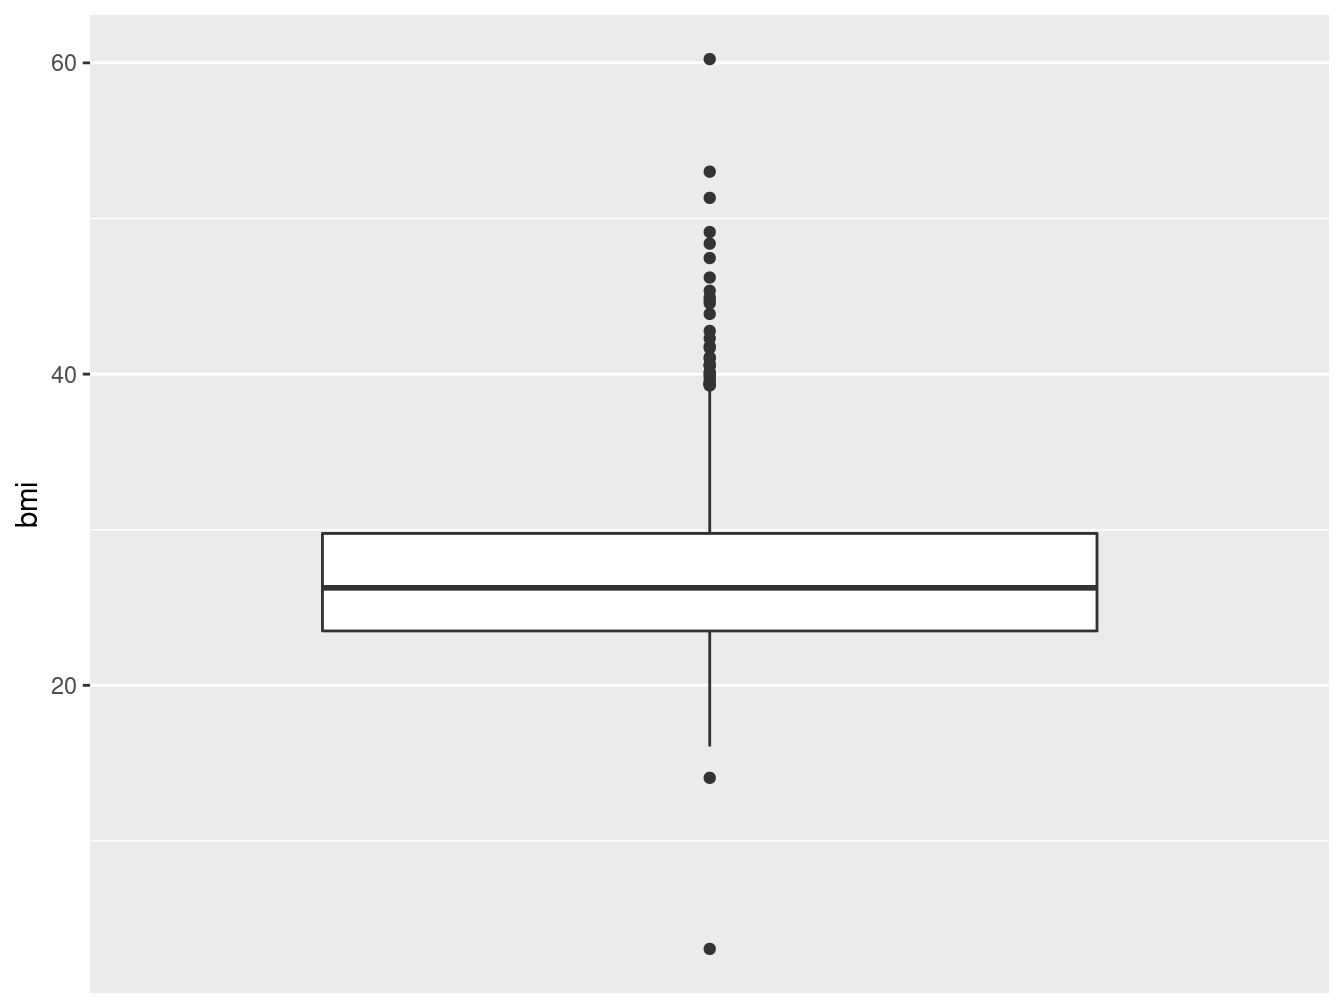
\includegraphics[width=0.8\linewidth]{01-scenario1_files/figure-latex/unnamed-chunk-50-1} \end{center}

\begin{Shaded}
\begin{Highlighting}[]
\OperatorTok{>}\StringTok{ }
\ErrorTok{>}\StringTok{ }\CommentTok{## geom_boxplot for boxplots by categorical}
\ErrorTok{>}\StringTok{ }\NormalTok{dat2 }\OperatorTok\StringTok{ }\KeywordTok{ggplot}\NormalTok{(}\KeywordTok{aes}\NormalTok{(}\DataTypeTok{x =}\NormalTok{ arm, }\DataTypeTok{y =}\NormalTok{ bmi)) }\OperatorTok{+}\StringTok{ }\KeywordTok{geom_boxplot}\NormalTok{() }\OperatorTok{+}\StringTok{ }\KeywordTok{labs}\NormalTok{(}\DataTypeTok{x =} \StringTok{"Treatment Arm"}\NormalTok{, }
\OperatorTok{+}\StringTok{     }\DataTypeTok{y =} \StringTok{"Age at Diagnosis"}\NormalTok{, }\DataTypeTok{title =} \StringTok{"Age with Treatment Group"}\NormalTok{, }\DataTypeTok{subtitle =} \StringTok{"This is a subtitle"}\NormalTok{, }
\OperatorTok{+}\StringTok{     }\DataTypeTok{caption =} \StringTok{"This is a caption"}\NormalTok{)}
\NormalTok{Warning}\OperatorTok{:}\StringTok{ }\NormalTok{Removed }\DecValTok{19}\NormalTok{ rows containing non}\OperatorTok{-}\NormalTok{finite }\KeywordTok{values}\NormalTok{ (stat_boxplot).}
\end{Highlighting}
\end{Shaded}

\begin{center}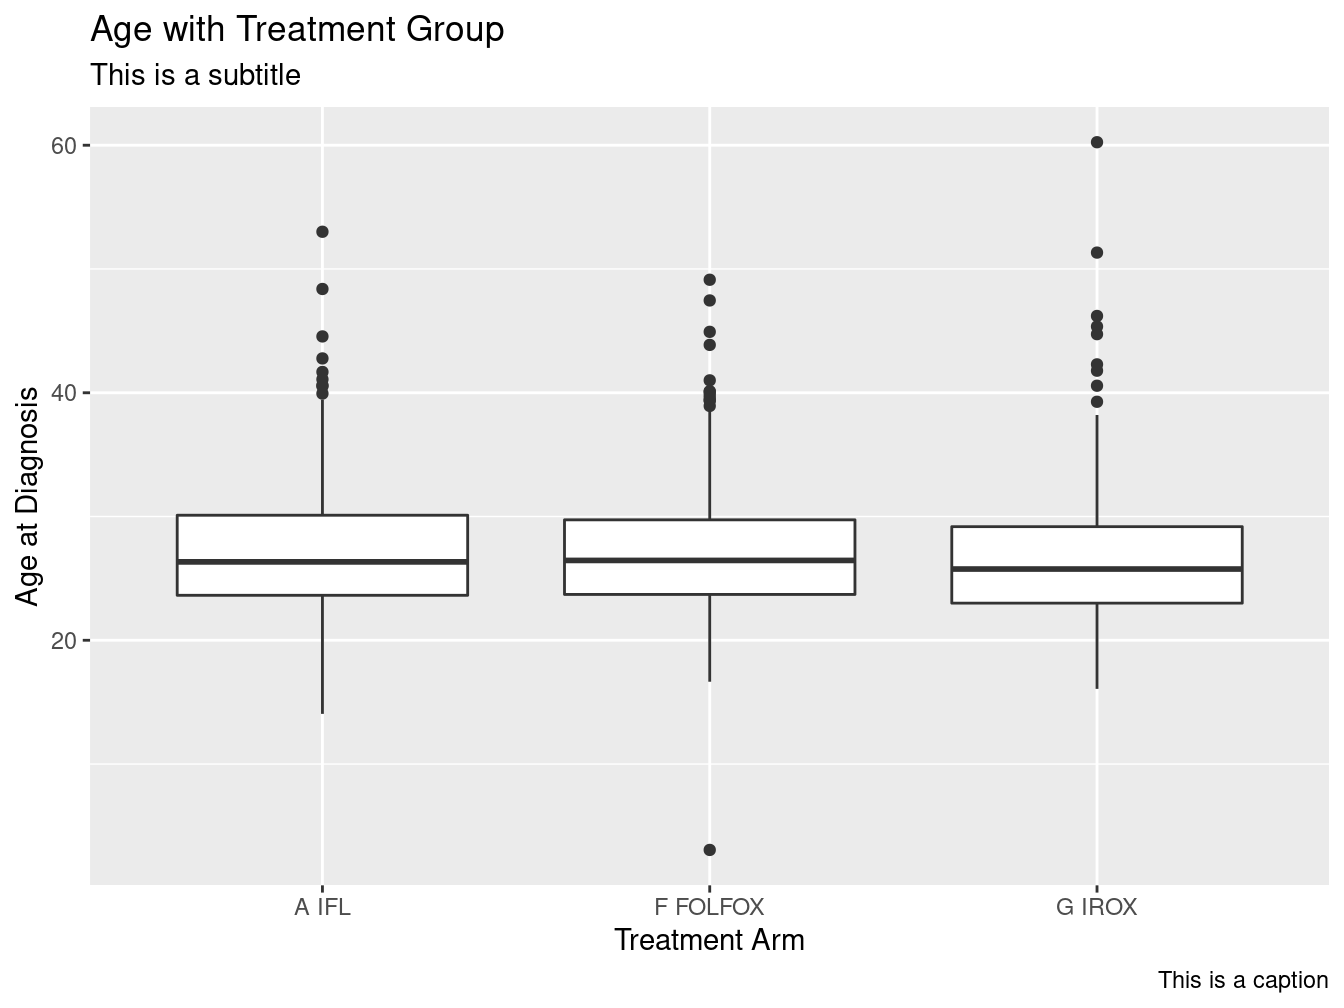
\includegraphics[width=0.8\linewidth]{01-scenario1_files/figure-latex/unnamed-chunk-50-2} \end{center}

\begin{Shaded}
\begin{Highlighting}[]
\OperatorTok{>}\StringTok{ }
\ErrorTok{>}\StringTok{ }\CommentTok{# this shows a different coloring scheme (theme_bw)}
\ErrorTok{>}\StringTok{ }\KeywordTok{ggplot}\NormalTok{(dat2, }\KeywordTok{aes}\NormalTok{(}\DataTypeTok{y =}\NormalTok{ bmi, }\DataTypeTok{x =}\NormalTok{ arm)) }\OperatorTok{+}\StringTok{ }\KeywordTok{geom_boxplot}\NormalTok{(}\DataTypeTok{fill =} \StringTok{"aliceblue"}\NormalTok{) }\OperatorTok{+}\StringTok{ }\KeywordTok{theme_bw}\NormalTok{() }\OperatorTok{+}\StringTok{ }
\OperatorTok{+}\StringTok{     }\KeywordTok{ggtitle}\NormalTok{(}\StringTok{"Boxplot of BMI by treatment arm"}\NormalTok{) }\OperatorTok{+}\StringTok{ }\KeywordTok{scale_y_continuous}\NormalTok{(}\DataTypeTok{name =} \StringTok{"BMI"}\NormalTok{, }
\OperatorTok{+}\StringTok{     }\DataTypeTok{breaks =} \KeywordTok{seq}\NormalTok{(}\DecValTok{0}\NormalTok{, }\DecValTok{70}\NormalTok{, }\DecValTok{10}\NormalTok{), }\DataTypeTok{limits =} \KeywordTok{c}\NormalTok{(}\DecValTok{0}\NormalTok{, }\DecValTok{70}\NormalTok{)) }\OperatorTok{+}\StringTok{ }\KeywordTok{scale_x_discrete}\NormalTok{(}\DataTypeTok{name =} \StringTok{"Treatment Arm"}\NormalTok{) }\OperatorTok{+}\StringTok{ }
\OperatorTok{+}\StringTok{     }\KeywordTok{theme}\NormalTok{(}\DataTypeTok{panel.grid.major =} \KeywordTok{element_line}\NormalTok{(}\DataTypeTok{colour =} \StringTok{"#e8e5e5"}\NormalTok{), }\DataTypeTok{panel.grid.minor =} \KeywordTok{element_blank}\NormalTok{(), }
\OperatorTok{+}\StringTok{         }\DataTypeTok{panel.border =} \KeywordTok{element_blank}\NormalTok{(), }\DataTypeTok{panel.background =} \KeywordTok{element_blank}\NormalTok{(), }\DataTypeTok{plot.title =} \KeywordTok{element_text}\NormalTok{(}\DataTypeTok{size =} \DecValTok{14}\NormalTok{, }
\OperatorTok{+}\StringTok{             }\DataTypeTok{face =} \StringTok{"bold"}\NormalTok{), }\DataTypeTok{axis.title =} \KeywordTok{element_text}\NormalTok{(}\DataTypeTok{face =} \StringTok{"bold"}\NormalTok{), }\DataTypeTok{axis.text.x =} \KeywordTok{element_text}\NormalTok{(}\DataTypeTok{colour =} \StringTok{"black"}\NormalTok{, }
\OperatorTok{+}\StringTok{             }\DataTypeTok{size =} \DecValTok{11}\NormalTok{), }\DataTypeTok{axis.text.y =} \KeywordTok{element_text}\NormalTok{(}\DataTypeTok{colour =} \StringTok{"black"}\NormalTok{, }\DataTypeTok{size =} \DecValTok{9}\NormalTok{), }\DataTypeTok{axis.line =} \KeywordTok{element_line}\NormalTok{(}\DataTypeTok{size =} \FloatTok{0.3}\NormalTok{, }
\OperatorTok{+}\StringTok{             }\DataTypeTok{colour =} \StringTok{"black"}\NormalTok{))}
\NormalTok{Warning}\OperatorTok{:}\StringTok{ }\NormalTok{Removed }\DecValTok{19}\NormalTok{ rows containing non}\OperatorTok{-}\NormalTok{finite }\KeywordTok{values}\NormalTok{ (stat_boxplot).}
\end{Highlighting}
\end{Shaded}

\begin{center}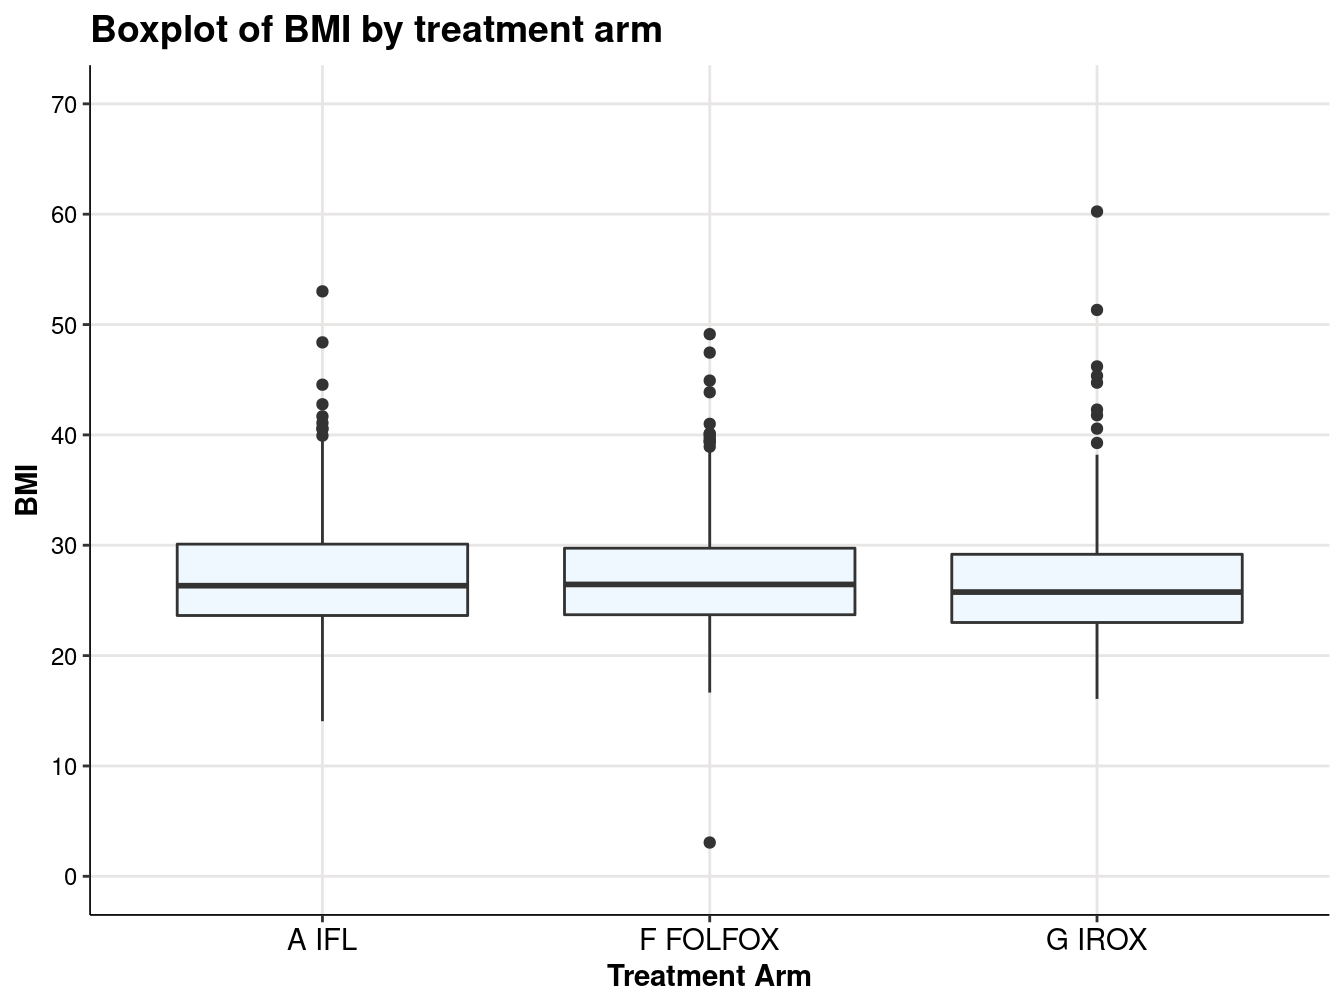
\includegraphics[width=0.8\linewidth]{01-scenario1_files/figure-latex/unnamed-chunk-50-3} \end{center}

\begin{itemize}
\tightlist
\item
  Now make two scatterplots side-by-side, split by sex
\end{itemize}

In addition to \texttt{facet\_grid()} and \texttt{facet\_wrap()} there is the \texttt{grid.arrange()} function which allows you to plot multiple figures on one page.

\begin{Shaded}
\begin{Highlighting}[]
\OperatorTok{>}\StringTok{ }\KeywordTok{library}\NormalTok{(gridExtra)}

\NormalTok{Attaching package}\OperatorTok{:}\StringTok{ 'gridExtra'}
\NormalTok{The following object is masked from }\StringTok{'package:dplyr'}\OperatorTok{:}

\StringTok{    }\NormalTok{combine}
\OperatorTok{>}\StringTok{ }
\ErrorTok{>}\StringTok{ }\NormalTok{plot1 <-}\StringTok{ }\KeywordTok{ggplot}\NormalTok{(}\KeywordTok{filter}\NormalTok{(dat2, sex }\OperatorTok{==}\StringTok{ "Female"}\NormalTok{), }\KeywordTok{aes}\NormalTok{(}\DataTypeTok{x =}\NormalTok{ age, }\DataTypeTok{y =}\NormalTok{ bmi, }\DataTypeTok{color =}\NormalTok{ arm)) }\OperatorTok{+}\StringTok{ }
\OperatorTok{+}\StringTok{     }\KeywordTok{geom_point}\NormalTok{() }\OperatorTok{+}\StringTok{ }\KeywordTok{ggtitle}\NormalTok{(}\StringTok{"Female Scatter Plot"}\NormalTok{)}
\OperatorTok{>}\StringTok{ }\NormalTok{plot2 <-}\StringTok{ }\KeywordTok{ggplot}\NormalTok{(}\KeywordTok{filter}\NormalTok{(dat2, sex }\OperatorTok{==}\StringTok{ "Male"}\NormalTok{), }\KeywordTok{aes}\NormalTok{(}\DataTypeTok{x =}\NormalTok{ age, }\DataTypeTok{y =}\NormalTok{ bmi, }\DataTypeTok{color =}\NormalTok{ arm)) }\OperatorTok{+}\StringTok{ }
\OperatorTok{+}\StringTok{     }\KeywordTok{geom_point}\NormalTok{() }\OperatorTok{+}\StringTok{ }\KeywordTok{ggtitle}\NormalTok{(}\StringTok{"Male Scatter Plot"}\NormalTok{)}
\OperatorTok{>}\StringTok{ }
\ErrorTok{>}\StringTok{ }\KeywordTok{grid.arrange}\NormalTok{(plot1, plot2, }\DataTypeTok{ncol =} \DecValTok{2}\NormalTok{)}
\NormalTok{Warning}\OperatorTok{:}\StringTok{ }\NormalTok{Removed }\DecValTok{7}\NormalTok{ rows containing missing }\KeywordTok{values}\NormalTok{ (geom_point).}
\NormalTok{Warning}\OperatorTok{:}\StringTok{ }\NormalTok{Removed }\DecValTok{12}\NormalTok{ rows containing missing }\KeywordTok{values}\NormalTok{ (geom_point).}
\end{Highlighting}
\end{Shaded}

\begin{center}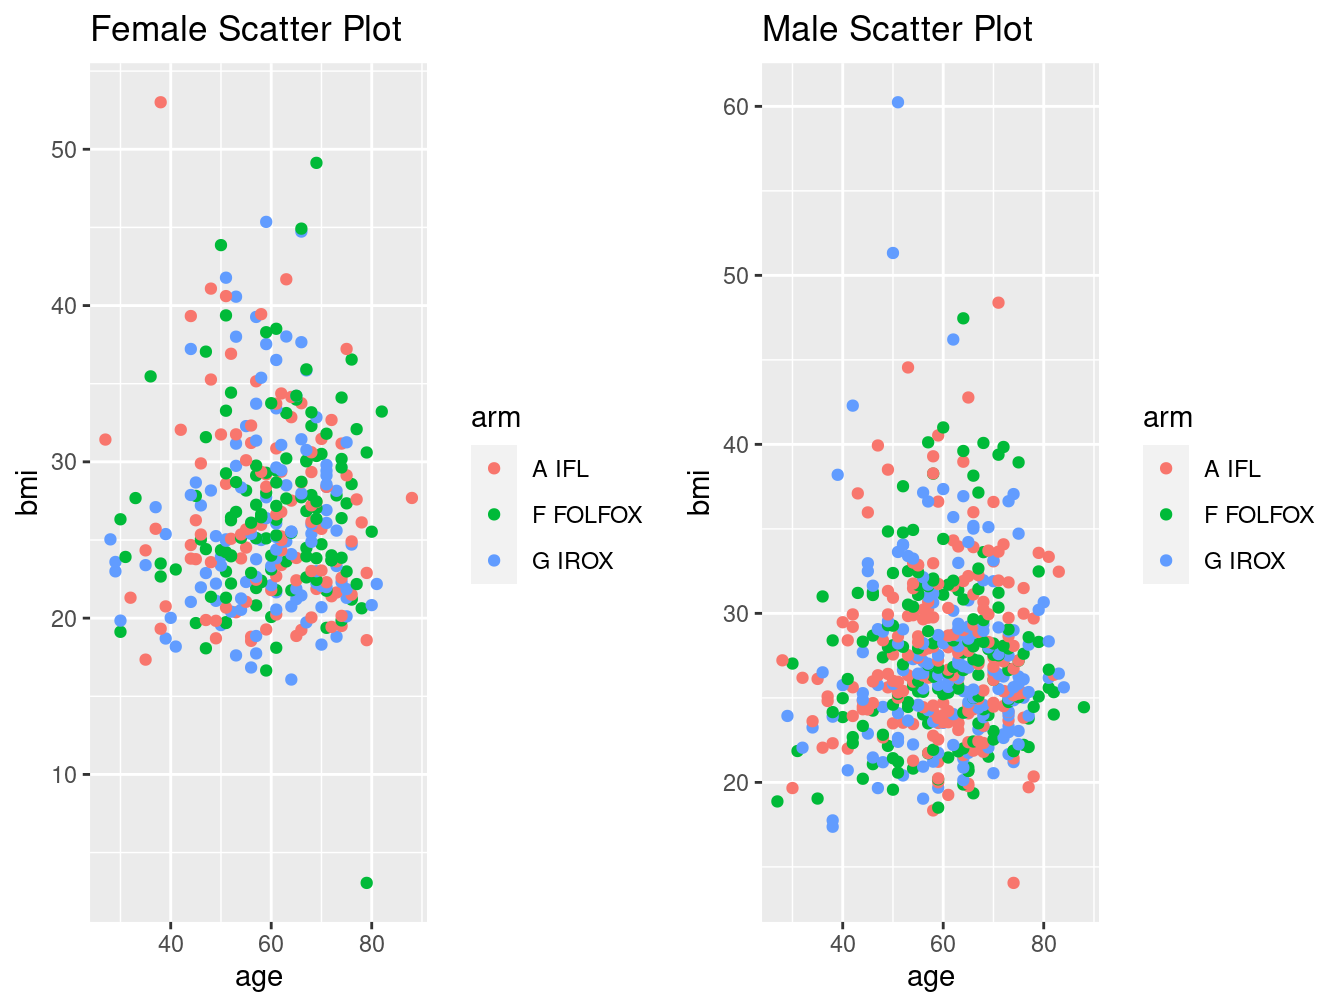
\includegraphics[width=0.8\linewidth]{01-scenario1_files/figure-latex/unnamed-chunk-51-1} \end{center}

\begin{Shaded}
\begin{Highlighting}[]
\OperatorTok{>}\StringTok{ }\KeywordTok{ggplot}\NormalTok{(dat2, }\KeywordTok{aes}\NormalTok{(}\DataTypeTok{x =}\NormalTok{ age, }\DataTypeTok{y =}\NormalTok{ bmi)) }\OperatorTok{+}\StringTok{ }\KeywordTok{geom_point}\NormalTok{() }\OperatorTok{+}\StringTok{ }\KeywordTok{theme_bw}\NormalTok{() }\OperatorTok{+}\StringTok{ }\KeywordTok{theme}\NormalTok{() }\OperatorTok{+}\StringTok{ }\KeywordTok{ggtitle}\NormalTok{(}\StringTok{"Scatterplot - Age by BMI"}\NormalTok{) }\OperatorTok{+}\StringTok{ }
\OperatorTok{+}\StringTok{     }\KeywordTok{labs}\NormalTok{(}\DataTypeTok{x =}\NormalTok{ vlabels}\OperatorTok{$}\NormalTok{age, }\DataTypeTok{y =}\NormalTok{ vlabels}\OperatorTok{$}\NormalTok{bmi) }\OperatorTok{+}\StringTok{ }\KeywordTok{facet_grid}\NormalTok{(. }\OperatorTok{~}\StringTok{ }\NormalTok{sex)}
\NormalTok{Warning}\OperatorTok{:}\StringTok{ }\NormalTok{Removed }\DecValTok{19}\NormalTok{ rows containing missing }\KeywordTok{values}\NormalTok{ (geom_point).}
\end{Highlighting}
\end{Shaded}

\begin{center}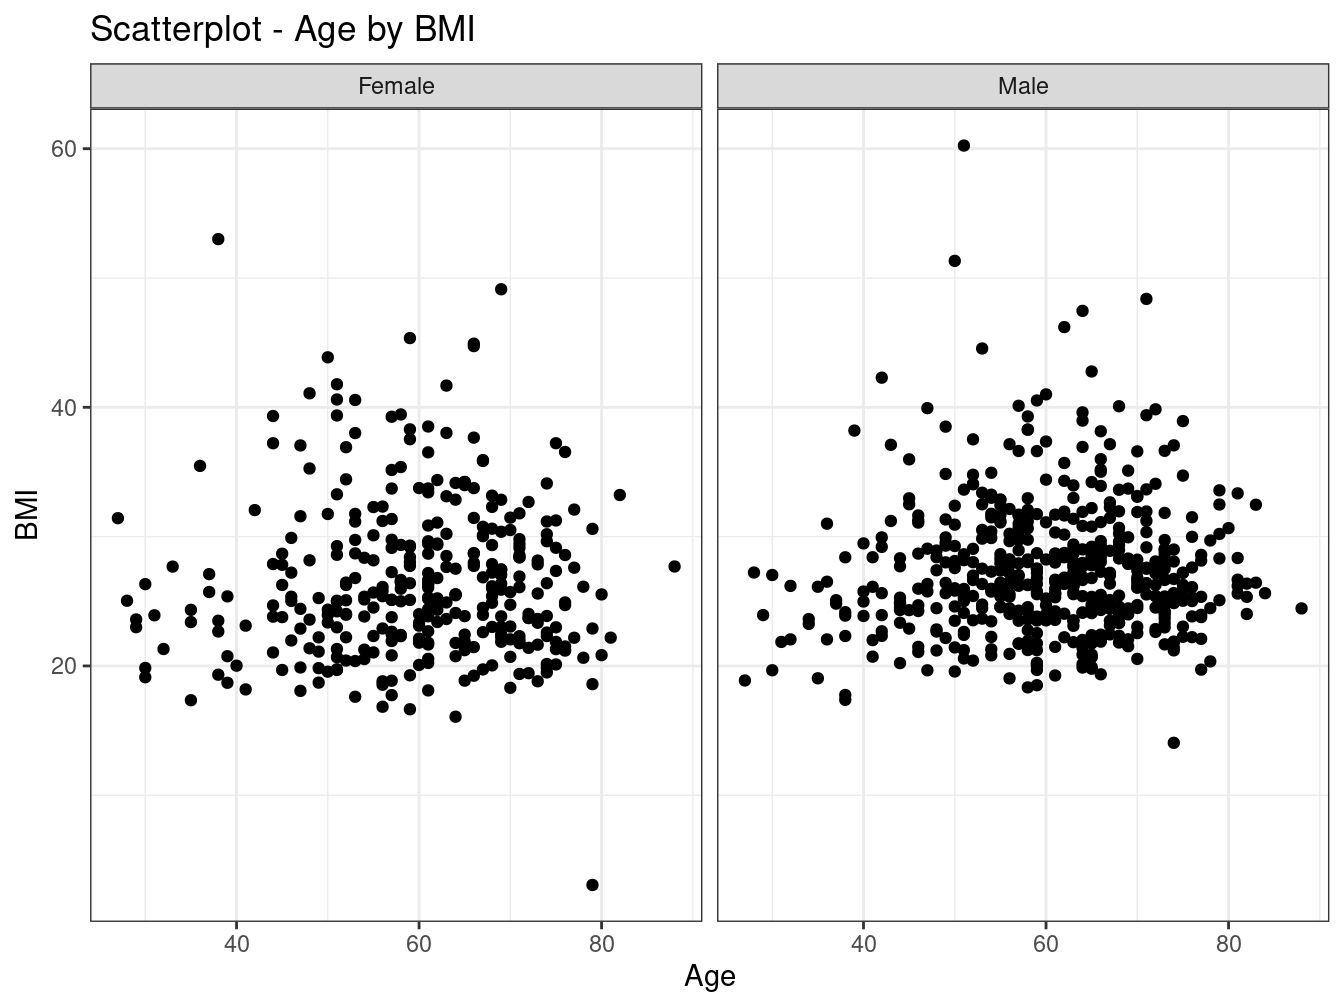
\includegraphics[width=0.8\linewidth]{01-scenario1_files/figure-latex/unnamed-chunk-52-1} \end{center}

\begin{itemize}
\tightlist
\item
  Fancier: How would you add a regression line to these plots? How about smoothers?
\end{itemize}

There are other packages that can do some of this work, but essentially this is how you would create these plots using base R graphics.

\begin{Shaded}
\begin{Highlighting}[]
\OperatorTok{>}\StringTok{ }\CommentTok{# code using basic R -- Regression lines}
\ErrorTok{>}\StringTok{ }\KeywordTok{par}\NormalTok{(}\DataTypeTok{mfrow =} \KeywordTok{c}\NormalTok{(}\DecValTok{1}\NormalTok{, }\DecValTok{2}\NormalTok{))}
\OperatorTok{>}\StringTok{ }\KeywordTok{plot}\NormalTok{(bmi }\OperatorTok{~}\StringTok{ }\NormalTok{age, }\DataTypeTok{data =}\NormalTok{ dat2[dat2}\OperatorTok{$}\NormalTok{sex }\OperatorTok{==}\StringTok{ "Female"}\NormalTok{, ], }\DataTypeTok{col =} \KeywordTok{as.numeric}\NormalTok{(}\KeywordTok{as.factor}\NormalTok{(arm)), }
\OperatorTok{+}\StringTok{     }\DataTypeTok{main =} \StringTok{"Females"}\NormalTok{)}
\OperatorTok{>}\StringTok{ }\KeywordTok{abline}\NormalTok{(}\KeywordTok{lm}\NormalTok{(bmi }\OperatorTok{~}\StringTok{ }\NormalTok{age, }\DataTypeTok{data =}\NormalTok{ dat2[dat2}\OperatorTok{$}\NormalTok{sex }\OperatorTok{==}\StringTok{ "Female"} \OperatorTok{&}\StringTok{ }\NormalTok{dat2}\OperatorTok{$}\NormalTok{arm }\OperatorTok{==}\StringTok{ "A IFL"}\NormalTok{, ]), }
\OperatorTok{+}\StringTok{     }\DataTypeTok{col =} \DecValTok{1}\NormalTok{)}
\OperatorTok{>}\StringTok{ }\KeywordTok{abline}\NormalTok{(}\KeywordTok{lm}\NormalTok{(bmi }\OperatorTok{~}\StringTok{ }\NormalTok{age, }\DataTypeTok{data =}\NormalTok{ dat2[dat2}\OperatorTok{$}\NormalTok{sex }\OperatorTok{==}\StringTok{ "Female"} \OperatorTok{&}\StringTok{ }\NormalTok{dat2}\OperatorTok{$}\NormalTok{arm }\OperatorTok{==}\StringTok{ "F FOLFOX"}\NormalTok{, ]), }
\OperatorTok{+}\StringTok{     }\DataTypeTok{col =} \DecValTok{2}\NormalTok{)}
\OperatorTok{>}\StringTok{ }\KeywordTok{abline}\NormalTok{(}\KeywordTok{lm}\NormalTok{(bmi }\OperatorTok{~}\StringTok{ }\NormalTok{age, }\DataTypeTok{data =}\NormalTok{ dat2[dat2}\OperatorTok{$}\NormalTok{sex }\OperatorTok{==}\StringTok{ "Female"} \OperatorTok{&}\StringTok{ }\NormalTok{dat2}\OperatorTok{$}\NormalTok{arm }\OperatorTok{==}\StringTok{ "G IROX"}\NormalTok{, ]), }
\OperatorTok{+}\StringTok{     }\DataTypeTok{col =} \DecValTok{3}\NormalTok{)}
\OperatorTok{>}\StringTok{ }
\ErrorTok{>}\StringTok{ }\KeywordTok{plot}\NormalTok{(bmi }\OperatorTok{~}\StringTok{ }\NormalTok{age, }\DataTypeTok{data =}\NormalTok{ dat2[dat2}\OperatorTok{$}\NormalTok{sex }\OperatorTok{==}\StringTok{ "Male"}\NormalTok{, ], }\DataTypeTok{col =} \KeywordTok{as.numeric}\NormalTok{(}\KeywordTok{as.factor}\NormalTok{(arm)), }
\OperatorTok{+}\StringTok{     }\DataTypeTok{main =} \StringTok{"Males"}\NormalTok{)}
\OperatorTok{>}\StringTok{ }\KeywordTok{abline}\NormalTok{(}\KeywordTok{lm}\NormalTok{(bmi }\OperatorTok{~}\StringTok{ }\NormalTok{age, }\DataTypeTok{data =}\NormalTok{ dat2[dat2}\OperatorTok{$}\NormalTok{sex }\OperatorTok{==}\StringTok{ "Male"} \OperatorTok{&}\StringTok{ }\NormalTok{dat2}\OperatorTok{$}\NormalTok{arm }\OperatorTok{==}\StringTok{ "A IFL"}\NormalTok{, ]), }\DataTypeTok{col =} \DecValTok{1}\NormalTok{)}
\OperatorTok{>}\StringTok{ }\KeywordTok{abline}\NormalTok{(}\KeywordTok{lm}\NormalTok{(bmi }\OperatorTok{~}\StringTok{ }\NormalTok{age, }\DataTypeTok{data =}\NormalTok{ dat2[dat2}\OperatorTok{$}\NormalTok{sex }\OperatorTok{==}\StringTok{ "Male"} \OperatorTok{&}\StringTok{ }\NormalTok{dat2}\OperatorTok{$}\NormalTok{arm }\OperatorTok{==}\StringTok{ "F FOLFOX"}\NormalTok{, ]), }
\OperatorTok{+}\StringTok{     }\DataTypeTok{col =} \DecValTok{2}\NormalTok{)}
\OperatorTok{>}\StringTok{ }\KeywordTok{abline}\NormalTok{(}\KeywordTok{lm}\NormalTok{(bmi }\OperatorTok{~}\StringTok{ }\NormalTok{age, }\DataTypeTok{data =}\NormalTok{ dat2[dat2}\OperatorTok{$}\NormalTok{sex }\OperatorTok{==}\StringTok{ "Male"} \OperatorTok{&}\StringTok{ }\NormalTok{dat2}\OperatorTok{$}\NormalTok{arm }\OperatorTok{==}\StringTok{ "G IROX"}\NormalTok{, ]), }\DataTypeTok{col =} \DecValTok{3}\NormalTok{)}
\OperatorTok{>}\StringTok{ }\KeywordTok{legend}\NormalTok{(}\StringTok{"topright"}\NormalTok{, }\DataTypeTok{legend =} \KeywordTok{c}\NormalTok{(}\StringTok{"A IFL"}\NormalTok{, }\StringTok{"F FOLFOX"}\NormalTok{, }\StringTok{"G IROX"}\NormalTok{), }\DataTypeTok{col =} \DecValTok{1}\OperatorTok{:}\DecValTok{3}\NormalTok{, }\DataTypeTok{lty =} \DecValTok{1}\NormalTok{, }
\OperatorTok{+}\StringTok{     }\DataTypeTok{bty =} \StringTok{"n"}\NormalTok{)}
\end{Highlighting}
\end{Shaded}

\begin{center}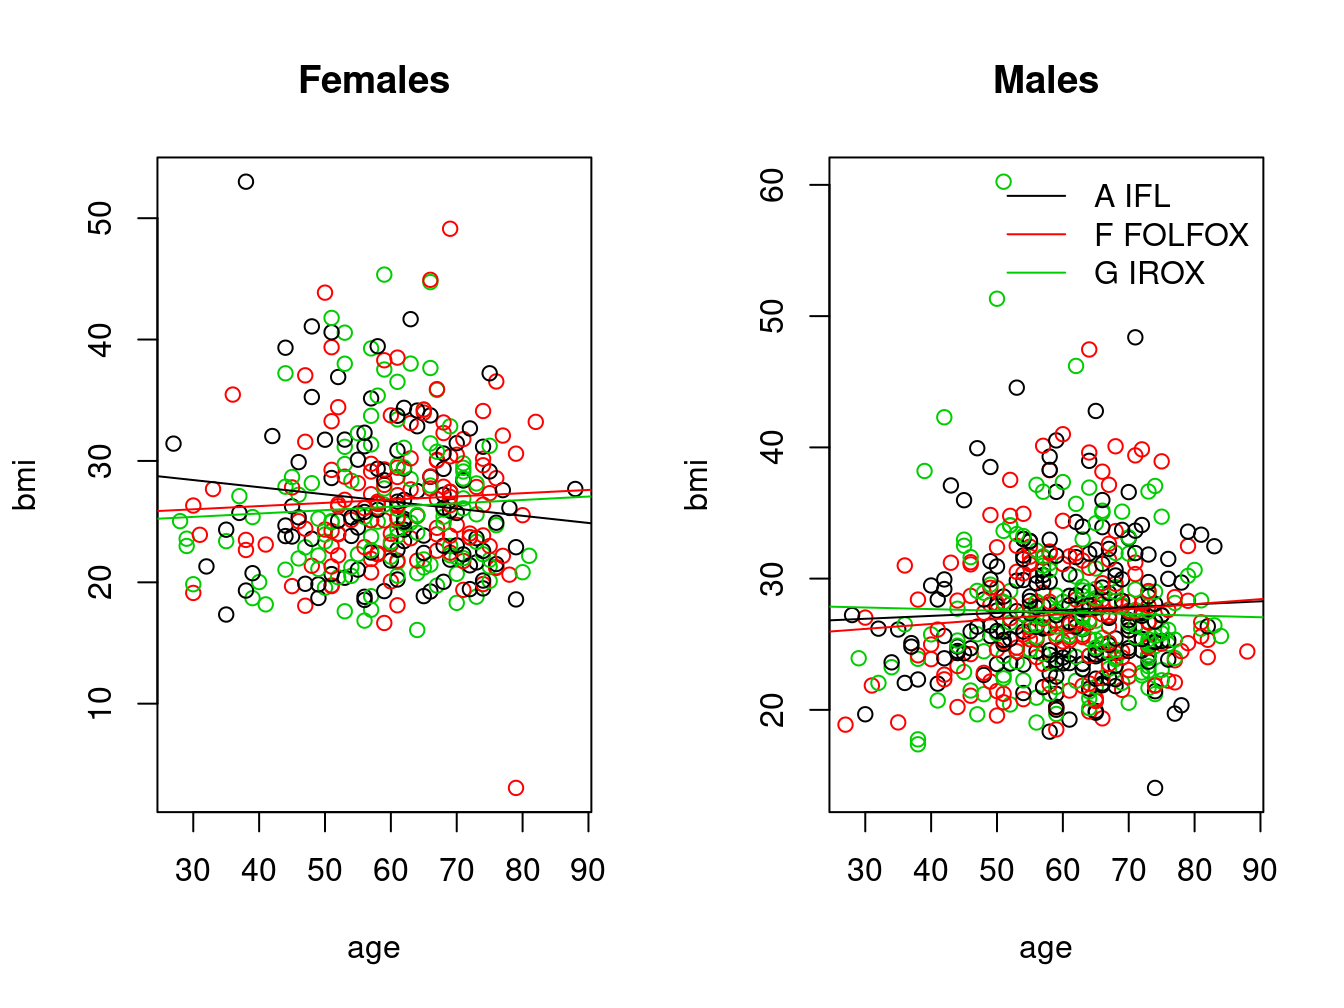
\includegraphics[width=0.8\linewidth]{01-scenario1_files/figure-latex/unnamed-chunk-53-1} \end{center}

\begin{Shaded}
\begin{Highlighting}[]
\OperatorTok{>}\StringTok{ }\KeywordTok{par}\NormalTok{(}\DataTypeTok{mfrow =} \KeywordTok{c}\NormalTok{(}\DecValTok{1}\NormalTok{, }\DecValTok{1}\NormalTok{))}
\OperatorTok{>}\StringTok{ }
\ErrorTok{>}\StringTok{ }\CommentTok{# -- Smoothers}
\ErrorTok{>}\StringTok{ }\KeywordTok{par}\NormalTok{(}\DataTypeTok{mfrow =} \KeywordTok{c}\NormalTok{(}\DecValTok{1}\NormalTok{, }\DecValTok{2}\NormalTok{))}
\OperatorTok{>}\StringTok{ }\CommentTok{# females}
\ErrorTok{>}\StringTok{ }\KeywordTok{plot}\NormalTok{(bmi }\OperatorTok{~}\StringTok{ }\NormalTok{age, }\DataTypeTok{data =}\NormalTok{ dat2[dat2}\OperatorTok{$}\NormalTok{sex }\OperatorTok{==}\StringTok{ "Female"}\NormalTok{, ], }\DataTypeTok{col =} \KeywordTok{as.numeric}\NormalTok{(}\KeywordTok{as.factor}\NormalTok{(arm)), }
\OperatorTok{+}\StringTok{     }\DataTypeTok{main =} \StringTok{"Females"}\NormalTok{)}
\OperatorTok{>}\StringTok{ }\NormalTok{tmp <-}\StringTok{ }\KeywordTok{na.omit}\NormalTok{(dat2[}\KeywordTok{which}\NormalTok{(dat2}\OperatorTok{$}\NormalTok{sex }\OperatorTok{==}\StringTok{ "Female"} \OperatorTok{&}\StringTok{ }\NormalTok{dat2}\OperatorTok{$}\NormalTok{arm }\OperatorTok{==}\StringTok{ "A IFL"}\NormalTok{), }\KeywordTok{c}\NormalTok{(}\StringTok{"bmi"}\NormalTok{, }\StringTok{"age"}\NormalTok{)])}
\OperatorTok{>}\StringTok{ }\KeywordTok{lines}\NormalTok{(}\KeywordTok{with}\NormalTok{(tmp, }\KeywordTok{smooth.spline}\NormalTok{(bmi }\OperatorTok{~}\StringTok{ }\NormalTok{age, }\DataTypeTok{spar =} \FloatTok{0.8}\NormalTok{)), }\DataTypeTok{col =} \DecValTok{1}\NormalTok{, }\DataTypeTok{lwd =} \DecValTok{2}\NormalTok{)}
\OperatorTok{>}\StringTok{ }
\ErrorTok{>}\StringTok{ }\NormalTok{tmp <-}\StringTok{ }\KeywordTok{na.omit}\NormalTok{(dat2[}\KeywordTok{which}\NormalTok{(dat2}\OperatorTok{$}\NormalTok{sex }\OperatorTok{==}\StringTok{ "Female"} \OperatorTok{&}\StringTok{ }\NormalTok{dat2}\OperatorTok{$}\NormalTok{arm }\OperatorTok{==}\StringTok{ "F FOLFOX"}\NormalTok{), }\KeywordTok{c}\NormalTok{(}\StringTok{"bmi"}\NormalTok{, }
\OperatorTok{+}\StringTok{     "age"}\NormalTok{)])}
\OperatorTok{>}\StringTok{ }\KeywordTok{lines}\NormalTok{(}\KeywordTok{with}\NormalTok{(tmp, }\KeywordTok{smooth.spline}\NormalTok{(bmi }\OperatorTok{~}\StringTok{ }\NormalTok{age, }\DataTypeTok{spar =} \FloatTok{0.8}\NormalTok{)), }\DataTypeTok{col =} \DecValTok{2}\NormalTok{, }\DataTypeTok{lwd =} \DecValTok{2}\NormalTok{)}
\OperatorTok{>}\StringTok{ }\NormalTok{tmp <-}\StringTok{ }\KeywordTok{na.omit}\NormalTok{(dat2[}\KeywordTok{which}\NormalTok{(dat2}\OperatorTok{$}\NormalTok{sex }\OperatorTok{==}\StringTok{ "Female"} \OperatorTok{&}\StringTok{ }\NormalTok{dat2}\OperatorTok{$}\NormalTok{arm }\OperatorTok{==}\StringTok{ "G IROX"}\NormalTok{), }\KeywordTok{c}\NormalTok{(}\StringTok{"bmi"}\NormalTok{, }
\OperatorTok{+}\StringTok{     "age"}\NormalTok{)])}
\OperatorTok{>}\StringTok{ }\KeywordTok{lines}\NormalTok{(}\KeywordTok{with}\NormalTok{(tmp, }\KeywordTok{smooth.spline}\NormalTok{(bmi }\OperatorTok{~}\StringTok{ }\NormalTok{age, }\DataTypeTok{spar =} \FloatTok{0.8}\NormalTok{)), }\DataTypeTok{col =} \DecValTok{3}\NormalTok{, }\DataTypeTok{lwd =} \DecValTok{2}\NormalTok{)}
\OperatorTok{>}\StringTok{ }
\ErrorTok{>}\StringTok{ }\CommentTok{# males}
\ErrorTok{>}\StringTok{ }\KeywordTok{plot}\NormalTok{(bmi }\OperatorTok{~}\StringTok{ }\NormalTok{age, }\DataTypeTok{data =}\NormalTok{ dat2[dat2}\OperatorTok{$}\NormalTok{sex }\OperatorTok{==}\StringTok{ "Male"}\NormalTok{, ], }\DataTypeTok{col =} \KeywordTok{as.numeric}\NormalTok{(}\KeywordTok{as.factor}\NormalTok{(arm)), }
\OperatorTok{+}\StringTok{     }\DataTypeTok{main =} \StringTok{"Males"}\NormalTok{)}
\OperatorTok{>}\StringTok{ }\NormalTok{tmp <-}\StringTok{ }\KeywordTok{na.omit}\NormalTok{(dat2[}\KeywordTok{which}\NormalTok{(dat2}\OperatorTok{$}\NormalTok{sex }\OperatorTok{==}\StringTok{ "Male"} \OperatorTok{&}\StringTok{ }\NormalTok{dat2}\OperatorTok{$}\NormalTok{arm }\OperatorTok{==}\StringTok{ "A IFL"}\NormalTok{), }\KeywordTok{c}\NormalTok{(}\StringTok{"bmi"}\NormalTok{, }\StringTok{"age"}\NormalTok{)])}
\OperatorTok{>}\StringTok{ }\KeywordTok{lines}\NormalTok{(}\KeywordTok{with}\NormalTok{(tmp, }\KeywordTok{smooth.spline}\NormalTok{(bmi }\OperatorTok{~}\StringTok{ }\NormalTok{age, }\DataTypeTok{spar =} \FloatTok{0.8}\NormalTok{)), }\DataTypeTok{col =} \DecValTok{1}\NormalTok{, }\DataTypeTok{lwd =} \DecValTok{2}\NormalTok{)}
\OperatorTok{>}\StringTok{ }
\ErrorTok{>}\StringTok{ }\NormalTok{tmp <-}\StringTok{ }\KeywordTok{na.omit}\NormalTok{(dat2[}\KeywordTok{which}\NormalTok{(dat2}\OperatorTok{$}\NormalTok{sex }\OperatorTok{==}\StringTok{ "Male"} \OperatorTok{&}\StringTok{ }\NormalTok{dat2}\OperatorTok{$}\NormalTok{arm }\OperatorTok{==}\StringTok{ "F FOLFOX"}\NormalTok{), }\KeywordTok{c}\NormalTok{(}\StringTok{"bmi"}\NormalTok{, }
\OperatorTok{+}\StringTok{     "age"}\NormalTok{)])}
\OperatorTok{>}\StringTok{ }\KeywordTok{lines}\NormalTok{(}\KeywordTok{with}\NormalTok{(tmp, }\KeywordTok{smooth.spline}\NormalTok{(bmi }\OperatorTok{~}\StringTok{ }\NormalTok{age, }\DataTypeTok{spar =} \FloatTok{0.8}\NormalTok{)), }\DataTypeTok{col =} \DecValTok{2}\NormalTok{, }\DataTypeTok{lwd =} \DecValTok{2}\NormalTok{)}
\OperatorTok{>}\StringTok{ }\NormalTok{tmp <-}\StringTok{ }\KeywordTok{na.omit}\NormalTok{(dat2[}\KeywordTok{which}\NormalTok{(dat2}\OperatorTok{$}\NormalTok{sex }\OperatorTok{==}\StringTok{ "Male"} \OperatorTok{&}\StringTok{ }\NormalTok{dat2}\OperatorTok{$}\NormalTok{arm }\OperatorTok{==}\StringTok{ "G IROX"}\NormalTok{), }\KeywordTok{c}\NormalTok{(}\StringTok{"bmi"}\NormalTok{, }\StringTok{"age"}\NormalTok{)])}
\OperatorTok{>}\StringTok{ }\KeywordTok{lines}\NormalTok{(}\KeywordTok{with}\NormalTok{(tmp, }\KeywordTok{smooth.spline}\NormalTok{(bmi }\OperatorTok{~}\StringTok{ }\NormalTok{age, }\DataTypeTok{spar =} \FloatTok{0.8}\NormalTok{)), }\DataTypeTok{col =} \DecValTok{3}\NormalTok{, }\DataTypeTok{lwd =} \DecValTok{2}\NormalTok{)}
\OperatorTok{>}\StringTok{ }
\ErrorTok{>}\StringTok{ }\CommentTok{# legend}
\ErrorTok{>}\StringTok{ }\KeywordTok{legend}\NormalTok{(}\StringTok{"topright"}\NormalTok{, }\DataTypeTok{legend =} \KeywordTok{c}\NormalTok{(}\StringTok{"A IFL"}\NormalTok{, }\StringTok{"F FOLFOX"}\NormalTok{, }\StringTok{"G IROX"}\NormalTok{), }\DataTypeTok{col =} \DecValTok{1}\OperatorTok{:}\DecValTok{3}\NormalTok{, }\DataTypeTok{lty =} \DecValTok{1}\NormalTok{, }
\OperatorTok{+}\StringTok{     }\DataTypeTok{bty =} \StringTok{"n"}\NormalTok{)}
\end{Highlighting}
\end{Shaded}

\begin{center}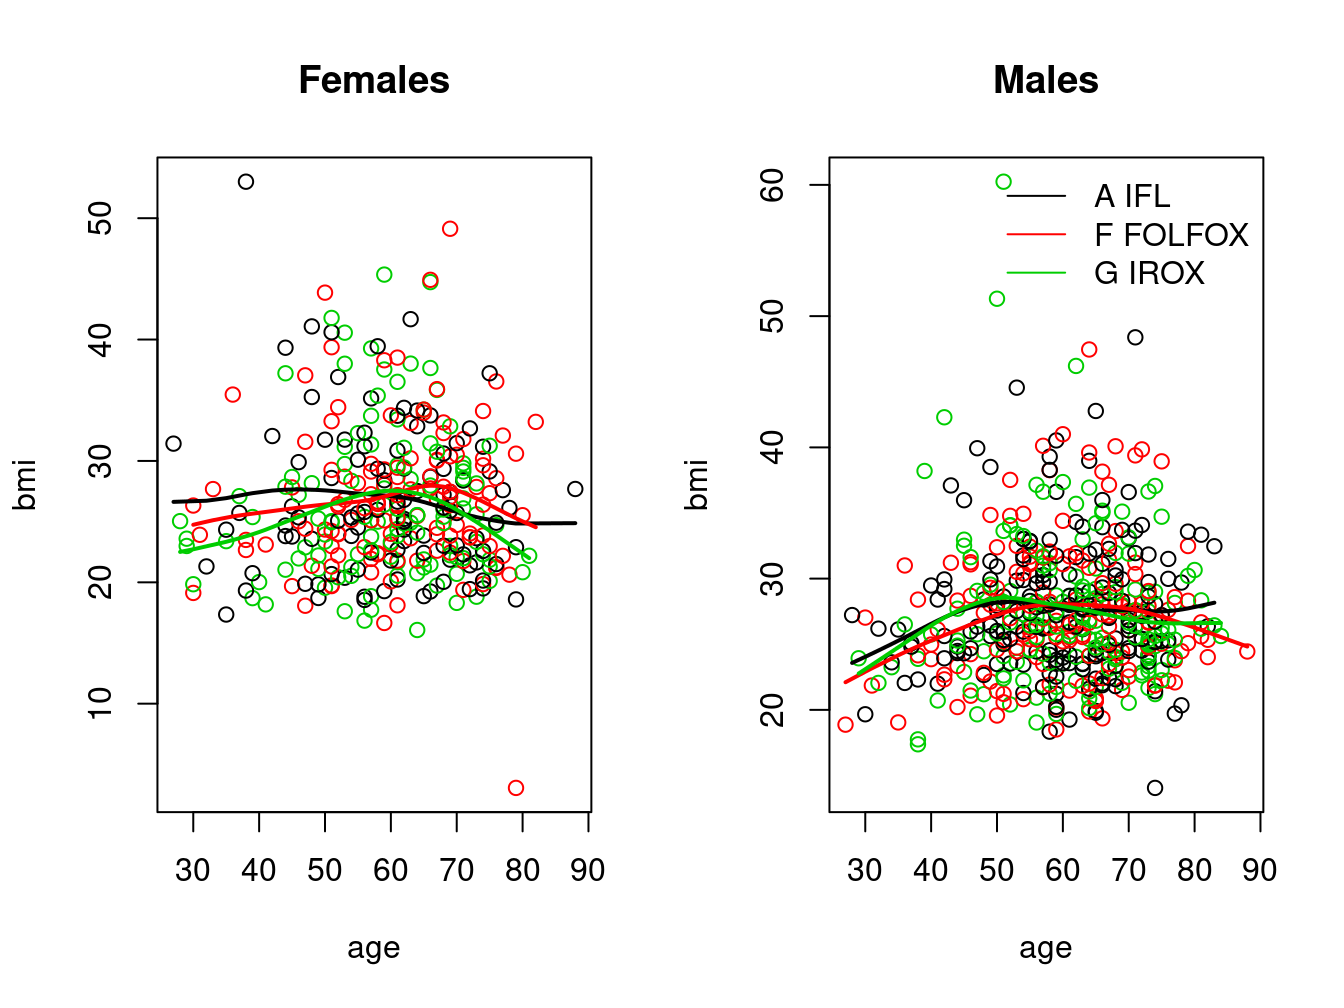
\includegraphics[width=0.8\linewidth]{01-scenario1_files/figure-latex/unnamed-chunk-53-2} \end{center}

\begin{Shaded}
\begin{Highlighting}[]
\OperatorTok{>}\StringTok{ }\KeywordTok{par}\NormalTok{(}\DataTypeTok{mfrow =} \KeywordTok{c}\NormalTok{(}\DecValTok{1}\NormalTok{, }\DecValTok{1}\NormalTok{))}
\end{Highlighting}
\end{Shaded}

\hypertarget{alt-model}{%
\subsection{Basic Modeling}\label{alt-model}}

There is a lot of information stored in a model object and \texttt{broom} doesn't work for all types of models. Sometimes you need to save the results from the summary of a fit which gives you different information than the fit itself.

\begin{Shaded}
\begin{Highlighting}[]
\OperatorTok{>}\StringTok{ }\CommentTok{# What is stored in the lm object?}
\ErrorTok{>}\StringTok{ }\KeywordTok{names}\NormalTok{(fit1)}
\NormalTok{ [}\DecValTok{1}\NormalTok{] }\StringTok{"coefficients"}  \StringTok{"residuals"}     \StringTok{"effects"}       \StringTok{"rank"}         
\NormalTok{ [}\DecValTok{5}\NormalTok{] }\StringTok{"fitted.values"} \StringTok{"assign"}        \StringTok{"qr"}            \StringTok{"df.residual"}  
\NormalTok{ [}\DecValTok{9}\NormalTok{] }\StringTok{"na.action"}     \StringTok{"xlevels"}       \StringTok{"call"}          \StringTok{"terms"}        
\NormalTok{[}\DecValTok{13}\NormalTok{] }\StringTok{"model"}        
\OperatorTok{>}\StringTok{ }
\ErrorTok{>}\StringTok{ }\CommentTok{# Now create a summary.lm object and see what is stored there}
\ErrorTok{>}\StringTok{ }\NormalTok{tmp <-}\StringTok{ }\KeywordTok{summary}\NormalTok{(fit1)}
\OperatorTok{>}\StringTok{ }\KeywordTok{names}\NormalTok{(tmp)}
\NormalTok{ [}\DecValTok{1}\NormalTok{] }\StringTok{"call"}          \StringTok{"terms"}         \StringTok{"residuals"}     \StringTok{"coefficients"} 
\NormalTok{ [}\DecValTok{5}\NormalTok{] }\StringTok{"aliased"}       \StringTok{"sigma"}         \StringTok{"df"}            \StringTok{"r.squared"}    
\NormalTok{ [}\DecValTok{9}\NormalTok{] }\StringTok{"adj.r.squared"} \StringTok{"fstatistic"}    \StringTok{"cov.unscaled"}  \StringTok{"na.action"}    
\OperatorTok{>}\StringTok{ }
\ErrorTok{>}\StringTok{ }\CommentTok{# Look at the model coefficients and p-values}
\ErrorTok{>}\StringTok{ }\NormalTok{tmp}\OperatorTok{$}\NormalTok{coefficients}
\NormalTok{              Estimate Std. Error   t value      }\KeywordTok{Pr}\NormalTok{(}\OperatorTok{>}\ErrorTok{|}\NormalTok{t}\OperatorTok{|}\NormalTok{)}
\NormalTok{(Intercept) }\FloatTok{25.6960705}  \FloatTok{0.6521116} \FloatTok{39.404408} \FloatTok{1.354488e-195}
\NormalTok{sex12        }\FloatTok{0.8783982}  \FloatTok{0.3886608}  \FloatTok{2.260064}  \FloatTok{2.406410e-02}
\OperatorTok{>}\StringTok{ }\KeywordTok{class}\NormalTok{(tmp}\OperatorTok{$}\NormalTok{coefficients)}
\NormalTok{[}\DecValTok{1}\NormalTok{] }\StringTok{"matrix"}
\end{Highlighting}
\end{Shaded}

\hypertarget{alt-revisited}{%
\subsection{Data Import, revisited}\label{alt-revisited}}

There are other packages that also read in Excel data including \texttt{openxlsx} and \texttt{gdata}. The package \texttt{xlsx} causes problems within RStudio and so users are strongly encouraged to no longer use that particular package. Note that \texttt{openxlsx} will only open newer \texttt{.xlsx} files. All three functions have slightly different options so if you need to do something fancy with Excel, it is worth looking more closely at the help pages.

\begin{Shaded}
\begin{Highlighting}[]
\OperatorTok{>}\StringTok{ }\CommentTok{# gdata}
\ErrorTok{>}\StringTok{ }\NormalTok{v1 <-}\StringTok{ }\NormalTok{gdata}\OperatorTok{::}\KeywordTok{read.xls}\NormalTok{(}\DataTypeTok{xls =} \StringTok{"data/dat1.xls"}\NormalTok{, }\DataTypeTok{sheet =} \DecValTok{1}\NormalTok{)}
\OperatorTok{>}\StringTok{ }
\ErrorTok{>}\StringTok{ }\CommentTok{# readxl}
\ErrorTok{>}\StringTok{ }\NormalTok{v2 <-}\StringTok{ }\NormalTok{readxl}\OperatorTok{::}\KeywordTok{read_excel}\NormalTok{(}\DataTypeTok{path =} \StringTok{"data/dat1.xls"}\NormalTok{, }\DataTypeTok{sheet =} \DecValTok{1}\NormalTok{)}
\OperatorTok{>}\StringTok{ }
\ErrorTok{>}\StringTok{ }\CommentTok{# openxlsx, cannot real .xls - only .xlsx v3 <-}
\ErrorTok{>}\StringTok{ }\CommentTok{# openxlsx::read.xlsx(xlsxFile='data/dat1.xls', sheet=1)}
\end{Highlighting}
\end{Shaded}

One of the differences between reading in SAS and Excel is that Excel doesn't have the concept of variable labels.

\begin{Shaded}
\begin{Highlighting}[]
\OperatorTok{>}\StringTok{ }\CommentTok{# Does the excel file have any variable labels?}
\ErrorTok{>}\StringTok{ }\KeywordTok{head}\NormalTok{(}\KeywordTok{labels}\NormalTok{(excel_dat1))}
\OperatorTok{$}\NormalTok{id}
\OtherTok{NULL}

\OperatorTok{$}\NormalTok{age}
\OtherTok{NULL}

\OperatorTok{$}\NormalTok{arm}
\OtherTok{NULL}

\OperatorTok{$}\NormalTok{sex}
\OtherTok{NULL}

\OperatorTok{$}\NormalTok{fu.time}
\OtherTok{NULL}

\OperatorTok{$}\NormalTok{fu.stat}
\OtherTok{NULL}
\OperatorTok{>}\StringTok{ }
\ErrorTok{>}\StringTok{ }\KeywordTok{head}\NormalTok{(}\KeywordTok{labels}\NormalTok{(sas_dat1))}
\OperatorTok{$}\NormalTok{id}
\OtherTok{NULL}

\OperatorTok{$}\NormalTok{age}
\OtherTok{NULL}

\OperatorTok{$}\NormalTok{arm}
\NormalTok{[}\DecValTok{1}\NormalTok{] }\StringTok{"Treatment Arm"}

\OperatorTok{$}\NormalTok{sex}
\OtherTok{NULL}

\OperatorTok{$}\NormalTok{fu.time}
\NormalTok{[}\DecValTok{1}\NormalTok{] }\StringTok{"Follow-up Time"}

\OperatorTok{$}\NormalTok{fu.stat}
\NormalTok{[}\DecValTok{1}\NormalTok{] }\StringTok{"Follow-up Status"}
\end{Highlighting}
\end{Shaded}

\hypertarget{appendix}{%
\chapter{Appendix}\label{appendix}}

\hypertarget{appendix-1-tidyverse-package-overviews}{%
\section{Appendix 1: tidyverse package overviews}\label{appendix-1-tidyverse-package-overviews}}

\hypertarget{dplyr}{%
\subsection{dplyr}\label{dplyr}}

The package \texttt{dplyr} focuses on transforming and summarizing tabular data with rows and columns. The package contains a set of functions (or ``verbs'') that perform common data manipulation operations such as filtering for rows, selecting specific columns, re-ordering rows, adding new columns and summarizing data. In addition, dplyr contains a useful function to perform another common task which is the ``split-apply-combine'' concept.

Important dplyr verbs to remember:

\begin{itemize}
\tightlist
\item
  \texttt{select()}: select certain columns (fields/variables) of your dataset
\item
  \texttt{filter()}: select specific rows (observations) of your dataset
\item
  \texttt{arrange()}: sort specified columns in ascending (default) or descending order\\
\item
  \texttt{mutate()}: add new columns or change existing ones
\item
  \texttt{summarise()}: summarise values
\item
  \texttt{group\_by()}: allows for group operations in the ``split-apply-combine'' concept
\item
  \texttt{rename()}: change column names for variables
\item
  \texttt{distinct()}: get unique values of specified variable set
\end{itemize}

Pipe operator: \texttt{\%\textgreater{}\%}

\begin{itemize}
\tightlist
\item
  dplyr imports this operator from another package (magrittr). This operator allows you to pipe the output from one function to the input of another function. Instead of nesting functions (reading from the inside to the outside), the idea of of piping is to read the functions from left to right.
\end{itemize}

Further examples are found at this \href{http://genomicsclass.github.io/book/pages/dplyr_tutorial.html}{dplyr tutorial}.

\hypertarget{tidyr}{%
\subsection{tidyr}\label{tidyr}}

The package \texttt{tidyr} focuses on transposing data, changing from a ``wide'' format to a ``long'' format.

Important tidyr verbs to remember:

\begin{itemize}
\tightlist
\item
  \texttt{pivot\_longer()} takes multiple columns, and gathers them into key-value pairs: it makes ``wide'' data longer (function used to be called \texttt{gather})
\item
  \texttt{pivot\_wider()} takes two columns (key \& value) and spreads in to multiple columns, it makes ``long'' data wider (function used to be called \texttt{spread})
\item
  \texttt{separate()} splits a single column into multiple columns
\item
  \texttt{unite()} combines multiple columns into a single column
\end{itemize}

Further examples are found at this \href{https://rpubs.com/bradleyboehmke/data_wrangling}{data wrangling site}.

\hypertarget{lubridate}{%
\subsection{lubridate}\label{lubridate}}

Historically dates have been challenging in R. The package \texttt{lubridate} helps with this and includes some basic date manipulation functions.

\begin{itemize}
\tightlist
\item
  \texttt{year(),\ month(),\ day()}: extract year, month, day
\item
  \texttt{hour(),\ minute(),\ second()}: extract hour, minute, second from a datetime variable
\item
  \texttt{date()}: extract date from datetime variable
\item
  \texttt{mdy()}: create date from text string
\end{itemize}

\begin{Shaded}
\begin{Highlighting}[]
\OperatorTok{>}\StringTok{ }\KeywordTok{library}\NormalTok{(lubridate)}
\OperatorTok{>}\StringTok{ }\KeywordTok{mdy}\NormalTok{(}\StringTok{"July 4th, 2000"}\NormalTok{)}
\NormalTok{[}\DecValTok{1}\NormalTok{] }\StringTok{"2000-07-04"}
\OperatorTok{>}\StringTok{ }\KeywordTok{mdy}\NormalTok{(}\StringTok{"7/4/2000"}\NormalTok{)}
\NormalTok{[}\DecValTok{1}\NormalTok{] }\StringTok{"2000-07-04"}
\end{Highlighting}
\end{Shaded}

\hypertarget{ggplot2}{%
\subsection{ggplot2}\label{ggplot2}}

The package \texttt{ggplot} focuses on displaying data graphically. It is based on the \texttt{grammer\ of\ graphics} (Wilkinson, 2005)

What Is The Grammar Of Graphics?

The basic idea: independently specify plot building blocks and combine them to create just about any kind of graphical display you want. Building blocks of a graph include:

\begin{itemize}
\tightlist
\item
  data - where is the data located
\item
  aesthetic mapping - what are your x, y, and grouping variables?\\
\item
  geometric object - what type of plot do you want to create
\item
  statistical transformations - log transform (or others)?
\item
  scales
\item
  coordinate system
\item
  position adjustments
\item
  faceting - creating separate figures ``by'' some value, but using the same scale, variables, labels, etc.
\item
  themes - color schemes used for plots, such as background color, axis defaults

  \begin{itemize}
  \tightlist
  \item
    \texttt{theme\_gray()} (default)
  \item
    \texttt{theme\_bw()}
  \item
    \texttt{theme\_classc()}
  \end{itemize}
\end{itemize}

\emph{Geometic Objects}

Geometric objects are the actual marks we put on a plot. Examples include:

\begin{itemize}
\tightlist
\item
  points (geom\_point, for scatter plots, dot plots, etc)
\item
  lines (geom\_line, for time series, trend lines, etc)
\item
  boxplot (geom\_boxplot, for boxplots)
\end{itemize}

A plot must have at least one geom; there is no upper limit. You can add a geom to a plot using the + operator

You can get a list of available geometric objects using the code below. There are also lots of examples of different types of plots available on the web (just include \texttt{ggplot} in your search).

\begin{verbatim}
help.search("geom_", package = "ggplot2")
\end{verbatim}

Try working through this \href{https://tutorials.iq.harvard.edu/R/Rgraphics/Rgraphics.html\#putting_it_all_together}{R graphics tutorial} to learn more.

\hypertarget{appendix-2-r-for-sas-programmers}{%
\section{Appendix 2: R for SAS programmers}\label{appendix-2-r-for-sas-programmers}}

If you tend to ``think SAS'', then making the switch to R can be challenging. A couple book that might help include:

\begin{itemize}
\tightlist
\item
  \emph{SAS and R: Data Management, Statistical Analysis, and Graphics} by Kleinman and Horton
\item
  \emph{R for SAS and SPSS Users} by Robert Muenchen
\end{itemize}

Below are a few select tasks and the packages/functions that handle those tasks.

\begin{table}

\caption{\label{tab:unnamed-chunk-2}Reading and Writing files}
\centering
\begin{tabular}[t]{l|l|l}
\hline
task & package & function\\
\hline
read SAS dataset & haven & read\_sas()\\
\hline
read csv dataset & readr & read\_csv()\\
\hline
read excel file & readxl & read\_excel()\\
\hline
read in multiple files & rlocal & read.all()\\
\hline
write csv file & readr & write\_csv()\\
\hline
write excel file & openxlsx & write.xlsx()\\
\hline
write object to Word/HTML/PDF & arsenal & write2word(), write2html(), write2pdf()\\
\hline
write text to file & base & sink()\\
\hline
print pretty markdown table & knitr & kable()\\
\hline
\end{tabular}
\end{table}

\begin{table}

\caption{\label{tab:unnamed-chunk-3}Manipulating data}
\centering
\begin{tabular}[t]{l|l|l}
\hline
task & package & function\\
\hline
summarize dataset & summarytools & dfSummary()\\
\hline
create data from m, d, y & arsenal & mdy.Date()\\
\hline
compare 2 datasets & arsenal & comparedf()\\
\hline
transpose data & tidyr & gather() and spread()\\
\hline
create categorical data from continuous & base & cut()\\
\hline
X in ('a','b','c') & base & \%in\%, match()\\
\hline
X NOT in ('a','b','c') & arsenal & \%nin\%\\
\hline
concatenate strings & base & paste0()\\
\hline
\end{tabular}
\end{table}

\begin{table}

\caption{\label{tab:unnamed-chunk-4}Modeling and Statistical Tests}
\centering
\begin{tabular}[t]{l|l|l}
\hline
task & package & function\\
\hline
table 1, unpaired data & arsenal & tableby()\\
\hline
table 1, paired data & arsenal & paired()\\
\hline
correlations & stats & cor.test()\\
\hline
partial correlations & ppcor & pcor.test()\\
\hline
binomial CI & rlocal & cibinom()\\
\hline
poisson CI & survival & cipoisson()\\
\hline
t-tests & stats & t.test()\\
\hline
Wilcoxon/Kolmogorov-Smirnov test & stats & wilcox.test(), ks.test()\\
\hline
linear regression & stats & lm()\\
\hline
logistic regression & stats & glm(, family=binomial)\\
\hline
poisson regression & stats & glm( , family=poisson)\\
\hline
negative binomial regression & MASS & glm.nb()\\
\hline
cox regression & survival & coxph()\\
\hline
quantile regression & quantreg & rq()\\
\hline
robust regression & MASS & rlm()\\
\hline
generalized additive regression & gam & gam()\\
\hline
create table from multiple models & arsenal & modelsum()\\
\hline
linear mixed effects (random slope) model & nlme & lme()\\
\hline
person-years analysis & survival & pyears()\\
\hline
incidence rates & rlocal & poprates()\\
\hline
\end{tabular}
\end{table}

  \bibliography{refer.bib}

\printindex

\end{document}
